\documentclass[11pt,oneside]{book}
\usepackage{fontspec}
\usepackage{xeCJK}
\setmainfont{Latin Modern Roman}
\setCJKmainfont[ItalicFont={Noto Serif CJK TC},BoldItalicFont={Noto Serif CJK TC Bold}]{Noto Serif CJK TC}
\setCJKsansfont{Noto Sans CJK TC}
\setCJKmonofont{Noto Sans Mono CJK TC}
\newfontfamily\proseunicodefont{DejaVu Serif}
\usepackage[margin=1in]{geometry}
\usepackage{microtype}
\usepackage{amsmath,amssymb,amsthm,mathtools,bm}
\usepackage{graphicx}
\usepackage{xcolor}
\usepackage{booktabs}
\usepackage{array}
\usepackage{longtable}
\usepackage{enumitem}
\usepackage{float}
\usepackage{caption}
\usepackage{hyperref}
\usepackage{fancyhdr}
\usepackage{tikz}
\usetikzlibrary{arrows.meta,positioning,calc,decorations.pathmorphing}

\hypersetup{
  colorlinks=true,
  linkcolor=blue!50!black,
  urlcolor=blue!50!black,
  citecolor=blue!50!black
}

\setlength{\parskip}{0.5em}
\setlength{\parindent}{0pt}
\setlist[itemize]{topsep=0.25em,itemsep=0.2em}
\setlist[enumerate]{topsep=0.25em,itemsep=0.2em}
\setlength{\headheight}{40pt}
\numberwithin{equation}{chapter}

\newtheorem{theorem}{定理}[chapter]
\newtheorem{proposition}[theorem]{命題}
\newtheorem{lemma}[theorem]{引理}
\newtheorem{corollary}[theorem]{推論}
\theoremstyle{definition}
\newtheorem{definition}[theorem]{定義}
\newtheorem{example}[theorem]{例}
\theoremstyle{remark}
\newtheorem{remark}[theorem]{註}

\providecommand{\ket}[1]{\left\lvert#1\right\rangle}
\providecommand{\bra}[1]{\left\langle#1\right\rvert}
\providecommand{\braket}[2]{\left\langle#1\,\middle|\,#2\right\rangle}
\providecommand{\expect}[1]{\left\langle#1\right\rangle}
\newcommand{\lectureoverview}[1]{\paragraph{概述。} #1}

\makeatletter
\newcommand{\course@headerfont}{\normalfont\small\itshape}
\newcommand{\course@pagefont}{\normalfont\small}
\newcommand{\course@headerraise}{14pt}
\newlength{\course@headerboxheight}
\setlength{\course@headerboxheight}{\dimexpr\headheight-\course@headerraise-9pt\relax}
\newcommand{\course@leftheadbox}[1]{%
  \raisebox{\course@headerraise}{%
    \parbox[t][\course@headerboxheight][t]{0.82\textwidth}{%
      \raggedright\course@headerfont\strut\MakeUppercase{#1}\strut%
    }%
  }%
}
\newcommand{\course@rightheadbox}[1]{%
  \raisebox{\course@headerraise}{%
    \parbox[t][\course@headerboxheight][t]{0.82\textwidth}{%
      \raggedleft\course@headerfont\strut\MakeUppercase{#1}\strut%
    }%
  }%
}
\renewcommand{\chaptermark}[1]{\markboth{\MakeUppercase{\chaptername\ \thechapter.\ #1}}{}}
\renewcommand{\sectionmark}[1]{\markright{\MakeUppercase{\thesection\hspace{0.4em}#1}}}
\fancyhf{}
\fancyhead[L]{\course@leftheadbox{\leftmark}}
\fancyhead[R]{\course@pagefont\thepage}
\renewcommand{\headrulewidth}{0.5pt}
\pagestyle{fancy}
\fancypagestyle{plain}{%
  \fancyhf{}
  \fancyhead[L]{\course@leftheadbox{\leftmark}}
  \fancyhead[R]{\course@pagefont\thepage}
  \renewcommand{\headrulewidth}{0.5pt}
}
\makeatother

% Video2Book editorial provenance macros
\newenvironment{classroomqa}{%
  \par\medskip\noindent\begin{minipage}{\linewidth}\small\hrule\medskip
}{%
  \medskip\hrule\end{minipage}\par\medskip
}
\newcommand{\audiencequestion}[1]{\noindent\textbf{聽眾提問。} #1\par\smallskip}
\newcommand{\lecturerresponse}[1]{\noindent\textbf{回答。} #1\par}
\newcommand{\lecturetimestamp}[1]{\footnote{講課時間： #1.}}
\newcommand{\lectureframe}[1]{\par\smallskip{\centering\footnotesize\itshape 講課畫面： #1.\par}}
\newcommand{\editorialnote}[1]{\footnote{編者說明： #1}}

\renewcommand{\contentsname}{目錄}
\renewcommand{\chaptername}{章}
\renewcommand{\figurename}{圖}
\renewcommand{\tablename}{表}
\renewcommand{\proofname}{證明}
\renewcommand{\bibname}{參考文獻}
\emergencystretch=2em
\pdfstringdefDisableCommands{\def\proseunicodefont{}}

\geometry{paperwidth=177.6mm,paperheight=252mm,left=16mm,right=16mm,
 top=18mm,bottom=18mm,includeheadfoot,headheight=28pt,headsep=7mm,footskip=9mm}
\usepackage{scrextend}
\changefontsizes[17pt]{12pt}
\raggedbottom
\renewenvironment{classroomqa}{\par\medskip\begingroup}{\par\endgroup\medskip}
\fancyhf{}
\setlength{\headwidth}{\textwidth}
\fancyhead[L]{\parbox{\textwidth}{\raggedright\fontsize{9}{11}\selectfont\nouppercase{\leftmark}}}
\fancyfoot[C]{\small\thepage}
\renewcommand{\headrulewidth}{0.3pt}
\fancypagestyle{plain}{\fancyhf{}\fancyfoot[C]{\small\thepage}\renewcommand{\headrulewidth}{0pt}}

\graphicspath{{../../../generated_course_notes/supplementary/particle_physics_1_basic_concepts/2009_fall/figures/}{../../../generated_course_notes/supplementary/particle_physics_1_basic_concepts/2009_fall/assets/}}
\begin{document}
\frontmatter
\hypersetup{pageanchor=false}
\begin{titlepage}
\hyphenpenalty=10000\exhyphenpenalty=10000
\thispagestyle{empty}
\begin{tikzpicture}[remember picture,overlay]
  \node[anchor=center,inner sep=0] at (current page.center) {%
    \includegraphics[height=\paperheight,keepaspectratio]{../../../generated_course_notes/supplementary/particle_physics_1_basic_concepts/2009_fall/assets/cover-art.png}%
  };
  \node[
    anchor=north west,
    align=left,
    text width=0.78\paperwidth,
    fill=white,
    fill opacity=0.9,
    rounded corners=8pt,
    inner xsep=10pt,
    inner ysep=8pt
  ] at ([xshift=0.08\paperwidth,yshift=-0.06\paperheight]current page.north west) {%
    {\fontsize{30}{33}\selectfont\bfseries\color{black!88} 粒子物理學（一）：基本概念\\[0.85em]}
    {\large\color{black!72} 繁體中文版 / 2009年秋季}
  };
  \node[
    anchor=south west,
    align=left,
    text width=0.68\paperwidth,
    fill=white,
    fill opacity=0.82,
    text opacity=1,
    rounded corners=6pt,
    inner sep=12pt
  ] at ([xshift=0.08\paperwidth,yshift=0.08\paperheight]current page.south west) {%
    {\normalsize\color{black!78} 原講授：Leonard Susskind\\[0.35em]}
    {\small\color{black!72} 講義輔助版本：\href{https://lazying.art}{LazyingArt LLC} / \href{https://github.com/lachlanchen/Video2Book}{Video2Book}}
  };
\end{tikzpicture}
\mbox{}
\end{titlepage}
\hypersetup{pageanchor=true}

\clearpage
\chapter*{關於本講義}
這些經獨立編輯的配套講義，依據 Leonard Susskind 的講課內容整理而成。內容是根據機器轉錄稿、字幕及部分黑板畫面重建，並對照可取得的來源資料核查。這些講義並非 Susskind 教授的原稿，也未經他審閱或認可。

本版由 \href{https://lazying.art}{LazyingArt LLC}採用開源的 \href{https://github.com/lachlanchen/Video2Book}{Video2Book} 工作流程編製。機器轉錄稿另行提供，其中可能有辨識錯誤。編輯上的釐清與重要重建均以腳註標示。
\clearpage
\tableofcontents
\mainmatter
\chapter{粒子、波與解析度所需的能量}

\section{粒子還是場？}

粒子物理學研究什麼？粒子---但這個答案立刻引出一個古老的問題：自然界是離散的嗎？這裡的「離散」是指物質由彼此分開、不可再分的單位構成，和「圓滑得體」毫無關係。希臘詞\emph{atom}的意思是「不可分割」，儘管如今稱為原子的物體可以再分。目前，\emph{粒子}將泛指離散的單位。

與此相對的是連續體的圖像。物質不再是彼此分離的部分所構成的集合，而是連續地散布在空間中。描述這種圖像，自然要用場的語言。場是位置的函數：物質的密度是一種場，電場和磁場也是場。後兩者決定帶電粒子的運動方式，但在經典觀點中，場本身被視為連續分布於空間。

不宜過度拘泥於這些觀念在歷史上的先後次序。這樣排列有助於呈現論證的邏輯，卻不代表它是可靠的年代順序。粒子的語彙包括原子、分子、碰撞和局域物體；連續體的語彙則包括場和連續變化的性質。哪一種圖像才正確？量子力學使兩者都不可能完全正確，但也使兩者都不可能全然錯誤。

這裡的討論會盡量自成一體，不過後續論證仍會用到量子力學、經典力學、狹義相對論和電磁學。眼前的問題比較簡單：最初是什麼使人們相信物質確實是離散的？

\section{物質離散性的化學證據}

至少在這套邏輯論述中，最初有力的證據來自化學，而非物理學。這種區分其實是人為的：化學在很大程度上就是原子與分子的物理學。道耳頓比較不同物質中相同數目的分子之質量。要確認樣本所含分子數相同，本身就是一大難題。此處會提到阿伏伽德羅；一莫耳所含的分子數就是阿伏伽德羅常數。若只是比較分子數相同的樣本，並不需要知道這個數的實際值。

引人注目的規律是：各物質的莫耳質量約為氫的莫耳質量的整數倍。這些倍數通常不是\(3/2\)、\(\pi\)或任意實數，而是接近整數的數。舉例來說，碳-12的質量約相當於十二個以氫為基準的質量單位。這強烈暗示物質是由質量幾乎相同的基本單位反覆組成。

現代的解釋消除了這個謎團。普通原子由質子、中子和電子構成。電子質量只有質子或中子的大約兩千分之一，因此對原子質量的貢獻很小。質子和中子幾乎承載了全部質量，而兩者的質量差遠小於百分之一。普通氫的原子核只有一個質子，因此原子或分子的質量約為氫尺度核質量的整數倍。這只是近似說法：質子和中子的質量並不完全相同，電子也有少量貢獻。儘管如此，這種近似整數的規律仍揭示了物質由離散成分構成。

後來，人們理解到分子是由原子組合而成。十九世紀的化學家辨認出約一百種原子，並將它們歸類為元素；若按基本的計數方式，約有九十二種元素天然存在，若再區分同位素，種類還會更多。週期表並不是按樸素的想法，簡單地重複相同大小的區塊，但它將這些不同物種整理了起來。在當時，各種元素本身看起來就是基本構成單位。愛因斯坦1905年的研究提供了定量方法，使物質的分子理論得到更有力的確立；不過，在此之前，化學證據已使原子圖像相當令人信服。

十九世紀末，這個看似終點的圖像不再成立。電子被發現，放射性也揭示了「元素就是基本單位」的圖像無法解釋的現象。放射性在微觀尺度上，已包含許多後來成為核物理與粒子物理核心的問題。

\section{放射性與分離的束流}

確切的歸屬和年代順序並不明確。一般會暫且將這項觀察歸於貝克勒爾：放射性物質恰好放在照相底片附近，並使底片受到影響，彷彿有不可見的輻射照射它。與其只把底片曝光視為受損，不如追問究竟是什麼到達了底片。瑪麗·居里後來的許多研究也屬於這段歷史，但若要理解實驗的邏輯，無須精確劃分早期各項發現的歸屬。

把材料放在厚實鉛塊的深處，並留出一條通往照相底片的窄通道。鉛的密度高，適合用來遮蔽輻射；通道則會準直逸出的輻射。底片上出現的不是一片模糊曝光，而是一個局部斑點，顯示輻射形成了有方向的束流。就這套論述的邏輯而言，這是第一束粒子束，雖然此時還不知道束流的本質。

接著讓準直後的輻射通過一個與軌跡平面垂直的磁場。曝光分成三支：一支不偏轉，繼續直行；另兩支向相反方向彎曲，而且偏轉量不同。電荷符號反轉時，磁力方向也會反轉，因此向相反方向彎曲的兩支表現出相反的電荷；直行的一支則表現為中性輻射。\footnote{此示意圖重現了講課影片中00:14:34至00:19:31之間畫出的圖。}

\begin{figure}[h]
\centering
\begin{tikzpicture}[scale=0.92]
\draw[fill=gray!20] (0,-1.55) rectangle (2.1,1.55);
\draw[fill=white,draw=none] (1.02,-0.13) rectangle (2.12,0.13);
\draw[fill=black] (1.02,0) circle (0.07);
\node[below] at (1.02,-0.12) {\small source};
\node[above] at (1.05,1.55) {\small lead};
\foreach \x in {3.0,3.55,4.1}
  \foreach \y in {-0.55,0,0.55}
    \node at (\x,\y) {\(\otimes\)};
\node[above] at (3.55,0.78) {\small \(\mathbf B\) into the page};
\draw[thick] (7,-1.8) -- (7,1.8);
\node[above] at (7,1.8) {\small plate};
\draw[thick,->] (2.1,0) -- (6.85,0);
\draw[thick,->] (2.1,0) .. controls (4.0,0.05) and (5.35,0.40) .. (6.85,0.88);
\draw[thick,->] (2.1,0) .. controls (3.7,-0.08) and (5.0,-0.75) .. (6.85,-1.42);
\node[right] at (7,0.88) {\small \(\alpha\)};
\node[right] at (7,0) {\small \(\gamma\)};
\node[right] at (7,-1.42) {\small \(\beta\)};
\end{tikzpicture}
\caption{橫向磁場中的準直放射性束流。中性成分不偏轉；帶相反電荷的成分則向相反方向彎曲，且偏轉量不同。}
\end{figure}

這三種成分分別稱為阿爾法、貝塔和伽馬。用現代術語來說，
\begin{equation}
\begin{aligned}
\beta\text{-radiation} &= \text{electrons},\\
\alpha\text{-radiation} &= \text{helium nuclei},\\
\gamma\text{-radiation} &= \text{photons}.
\end{aligned}
\end{equation}
阿爾法粒子含有兩個質子和兩個中子，因此質量數為四。在道耳頓近似的整數序列中，氦因此會排在第四位：相當於四個氫尺度的核質量單位。貝塔射線是帶負電的電子，人們早已從陰極射線實驗中認識電子。伽馬射線不帶電。

若放射源足夠稀薄，且探測器能分辨個別的到達事件，看似連續的曝光就會呈現為一連串分開的事件：閃一下、再閃一下、又閃一下。貝塔、阿爾法和伽馬輻射也都可以如此觀測。蓋革計數器能呈現這種情形，至於最早的裝置是否確實在這種條件下操作，則是另一回事。每種成分都是以離散的束包抵達。伽馬射線仍是個謎：它是中性的，卻一次只探測到一個事件。伽馬輻射是能量極高的光，而普朗克、尤其是愛因斯坦，將光與量子聯繫起來。不過，在面對這個結論之前，必須先認真看待光具有波動性的經典證據。

\section{光的經典波動性}

在經典物理中，光是連續性的典型例子。它由電場和磁場構成，並以連續波的形式傳播。牛頓曾支持微粒說，但波動實驗使波動說取而代之。電荷振盪會產生電磁輻射。宏觀天線可以發射無線電波、微波、紅外線、可見光或紫外線；原子內部運動的電荷也相當於一支天線。所發出的輻射可以使照相底片曝光。

單狹縫提供了波動行為的初步線索。如果光是子彈流，穿過小孔後應會形成邊緣清晰、準直的光點。然而，實際照明會擴散成一片模糊區域。不過，光的擴散本身還不足以定論，因為也可以設想粒子受到孔徑邊緣的力而偏轉。

雙狹縫提供了更明確的檢驗。兩束彼此獨立的粒子流會形成兩片重疊的散布區域，重疊處或許最亮。波的表現則不同：一個狹縫傳來的波峰可以遇上另一個狹縫傳來的波峰，彼此增強；波峰也可以遇上波谷，彼此抵消。因此，螢幕上會出現明暗相間的條紋，其中甚至有些暗處，若只有任一狹縫開啟，本來都會被照亮。\footnote{此示意圖重現了講課影片中00:25:00至00:29:49之間畫出的孔徑與干涉圖。}

\begin{figure}[h]
\centering
\resizebox{\linewidth}{!}{%
\begin{tikzpicture}[scale=0.88]
\begin{scope}
\draw[->] (-0.3,1.06) -- (0.8,1.06);
\draw[thick] (1.3,0.15) -- (1.3,0.92);
\draw[thick] (1.3,1.20) -- (1.3,2.0);
\draw[thick] (4.8,0.15) -- (4.8,2.0);
\draw[->] (1.34,1.06) .. controls (2.2,1.55) and (3.2,1.55) .. (4.65,1.48);
\draw[->] (1.34,1.06) -- (4.65,1.06);
\draw[->] (1.34,1.06) .. controls (2.2,0.58) and (3.2,0.58) .. (4.65,0.64);
\draw[dashed] (5.45,1.06) ellipse (0.47 and 0.82);
\node at (2.95,2.28) {\small one opening};
\node at (5.45,2.05) {\small broadened spot};
\end{scope}
\begin{scope}[xshift=6.8cm]
\draw[->] (-0.3,1.35) -- (0.8,1.35);
\draw[->] (-0.3,0.75) -- (0.8,0.75);
\draw[thick] (1.3,0.15) -- (1.3,0.62);
\draw[thick] (1.3,0.88) -- (1.3,1.25);
\draw[thick] (1.3,1.51) -- (1.3,2.0);
\draw[thick] (4.8,0.15) -- (4.8,2.0);
\draw[thin] (4.8,0.32) -- (5.18,0.32);
\draw[line width=2pt] (4.8,0.59) -- (5.18,0.59);
\draw[thin] (4.8,0.86) -- (5.18,0.86);
\draw[line width=2pt] (4.8,1.13) -- (5.18,1.13);
\draw[thin] (4.8,1.40) -- (5.18,1.40);
\draw[line width=2pt] (4.8,1.67) -- (5.18,1.67);
\draw[thin] (4.8,1.94) -- (5.18,1.94);
\draw[->] (1.34,0.75) .. controls (2.4,0.82) and (3.5,1.02) .. (4.65,1.13);
\draw[->] (1.34,1.38) .. controls (2.4,1.31) and (3.5,1.20) .. (4.65,1.13);
\draw[->] (1.34,0.75) .. controls (2.4,1.05) and (3.5,1.55) .. (4.65,1.67);
\draw[->] (1.34,1.38) .. controls (2.4,1.55) and (3.5,1.66) .. (4.65,1.67);
\node at (2.95,2.28) {\small two openings};
\node at (5.62,1.13) {\small bright and dark bands};
\end{scope}
\end{tikzpicture}
}
\caption{單一孔徑會使影像展寬；兩個孔徑則產生明暗相間的條紋，分別對應建設性與破壞性干涉。}
\end{figure}

很容易用水面來想像同樣的效應。用兩根手指撥動水面：圓形波紋向外傳開，在某些位置相互增強，在另一些位置相互抵消。決定性的波動特徵是干涉，而不只是擴散。

歷史脈絡同樣不簡單。在這套示意性的敘述中，惠更斯被安排在牛頓之前，代表波傳播的倡議者；托馬斯·楊則與干涉演示相連。牛頓的一些光學實驗也可以用波的干涉來解釋，儘管他本人支持微粒說。後來的干涉實驗確立了光的波動性，已無合理疑問。

接著，麥克斯韋指出究竟是什麼在振盪。若光波沿某一軸傳播，電場便垂直於該軸。磁場也垂直於該軸，並且與電場互相垂直。整個波的圖樣以光速傳播。\footnote{此示意圖重現了講課影片在00:31:08畫出的電磁波圖。}

\begin{figure}[h]
\centering
\begin{tikzpicture}[
  scale=0.9,
  x={(1cm,0cm)},
  y={(0cm,1cm)},
  z={(0.42cm,0.34cm)}
]
\draw[->] (0,0,0) -- (7,0,0) node[right] {\small propagation};
\draw[->] (0,-1.35,0) -- (0,1.35,0) node[above] {\small \(\mathbf E\)};
\draw[->] (0,0,-1.35) -- (0,0,1.35) node[above right] {\small \(\mathbf B\)};
\draw[thick,smooth,variable=\x,domain=0:6.3,samples=100]
  plot ({\x},{sin(\x r)},0);
\draw[thick,dashed,smooth,variable=\x,domain=0:6.3,samples=100]
  plot ({\x},0,{sin(\x r)});
\end{tikzpicture}
\caption{在電磁波中，電場與磁場彼此垂直，且兩者都垂直於傳播方向。}
\end{figure}

普通可見光的振盪快得無法直接追蹤其交變場。若是波長極長的無線電波，振盪也會相應地慢得多。無論哪一種情況，同樣的橫波幾何關係都會產生干涉。

\section{波長、週期與頻率}

波長\(\lambda\)是空間距離：從振盪中的某一點出發，沿著波前進，直到經過一個完整週期後，同一相位再次出現。波長以公尺、公分或其他長度單位表示。

現在停在某個位置，觀察波經過。完成一個完整週期所需的時間稱為週期\(T\)。可見光的週期極短，大約是\(10^{-15}\,\mathrm{s}\)的量級；波長越長，週期也越長，波長越短，週期也越短。

波在一個週期內前進一個波長，因此速度為\(v\)的波滿足
\begin{equation}
v=\frac{\lambda}{T}.
\end{equation}
水波和聲波各有自己的傳播速度。對光而言，
\begin{equation}
c=\frac{\lambda}{T}.
\end{equation}
頻率\(f\)是單位時間內完成的週期數：
\begin{equation}
f=\frac{1}{T}.
\end{equation}
因此
\begin{equation}
\lambda f=c.
\end{equation}
知道波長或頻率其中之一，就能決定另一個。

\begin{figure}[h]
\centering
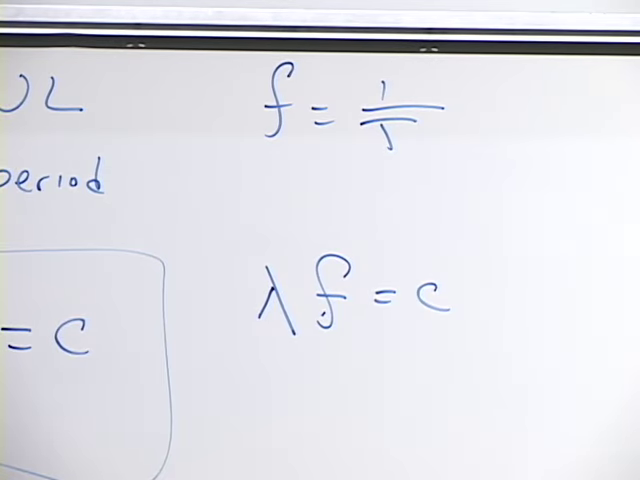
\includegraphics[width=0.68\textwidth]{lecture_01_figure_03.png}
\caption{對光波而言，\(f=1/T\)，而且\(\lambda f=c\)。}
\lectureframe{00:36:24}
\end{figure}

物理學家常以每秒弧度數，而非每秒完整週期數，來表示振盪速率。想像一個點沿圓周做等速運動。若該點每秒繞行\(f\)圈，而每圈包含\(2\pi\)弧度，其角頻率便是
\begin{equation}
\omega=2\pi f,
\qquad
\frac{\omega}{2\pi}=f.
\end{equation}
目前這只是定義；至於這種表示法實際上是否能減少\(2\pi\)因子的數目，稍後再談。

結合\(f=c/\lambda\)與\(\omega=2\pi f\)，得到
\begin{equation}
\omega=\frac{2\pi c}{\lambda},
\qquad
\omega\lambda=2\pi c.
\end{equation}
若考慮其他種類的波，式中的\(c\)就換成該波的傳播速度。

\begin{figure}[h]
\centering
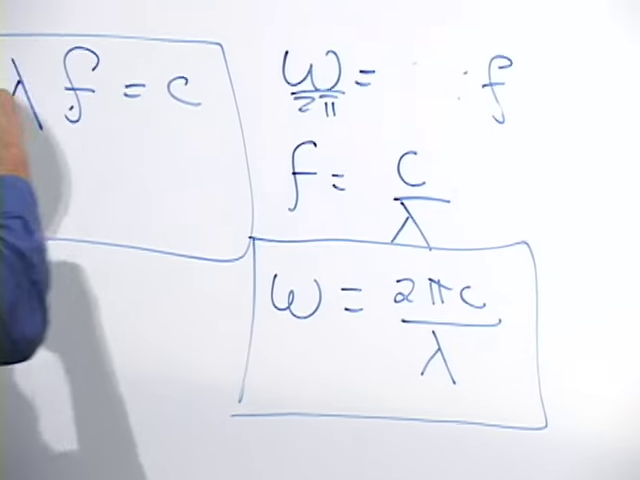
\includegraphics[width=0.68\textwidth]{lecture_01_figure_04.png}
\caption{對於\(\omega=2\pi f\)，光波滿足\(\omega=2\pi c/\lambda\)。}
\lectureframe{00:39:10}
\end{figure}

電磁輻射形成連續光譜。按波長由長至短排列，慣用名稱如下：
\begin{equation}
\begin{aligned}
\text{radio}
&\longrightarrow \text{microwave}
\longrightarrow \text{infrared}
\longrightarrow \text{visible}\\
&\longrightarrow \text{ultraviolet}
\longrightarrow \text{X ray}
\longrightarrow \text{gamma ray}.
\end{aligned}
\end{equation}
可見光只占其中一小段。各名稱所指區域之間的界線是約定俗成的，因此此處不必指定精確的分界波長。無線電波的波長可以極長；伽馬輻射則位於電磁光譜中波長極短的一端。現在問題變得鮮明：伽馬輻射在經典理論中是連續的場波，卻以離散的閃光事件被探測到。

\section{離散到達事件與波的機率}

從輻射的熱力學性質出發，普朗克和愛因斯坦得出結論：必須將光視為由離散單位構成。這個假想實驗能生動說明這一點，但不代表實際的歷史發現過程就是如此。

讓一束光照在螢幕上。一般強度下，光會形成一片看似連續的亮斑。在光束中放入部分不透明的衰減片，亮斑就會變暗。逐步加強衰減，每單位時間到達的光便越來越少。最後，亮斑的樣貌會改變：探測器記錄到的不再是連續變暗的光斑，而是一個個孤立事件。\footnote{此示意圖重現了講課影片中00:42:32至00:45:42之間講解的衰減實驗。}

\begin{figure}[h]
\centering
\begin{tikzpicture}[scale=0.9]
\begin{scope}
\draw[fill=yellow!35] (0,0) circle (0.18);
\draw[->,thick] (0.2,0) -- (2.55,0);
\draw[thick] (2.65,-1.0) -- (2.65,1.0);
\node[below] at (1.4,-1.0) {\small bright beam};
\end{scope}
\begin{scope}[xshift=4.1cm]
\draw[fill=yellow!35] (0,0) circle (0.18);
\draw[->,thick] (0.2,0) -- (1.15,0);
\draw[fill=gray!70] (1.2,-0.85) rectangle (1.55,0.85);
\draw[->,thick] (1.6,0) -- (2.55,0);
\draw[thick] (2.65,-1.0) -- (2.65,1.0);
\node[below] at (1.85,-1.0) {\small strong attenuation};
\end{scope}
\fill[gray!45] (2.62,-0.65) rectangle (2.70,0.65);
\foreach \y in {-0.66,-0.31,0.13,0.58}
  \fill (6.72,\y) circle (0.045);
\node[above] at (2.65,1.0) {\small unresolved exposure};
\node[above] at (6.75,1.0) {\small isolated detections};
\end{tikzpicture}
\caption{逐步衰減會降低探測率，直到看似連續的曝光分解為孤立的光子事件。}
\end{figure}

等待足夠久，這些事件累積起來後，會呈現出與原來光斑相同的空間分布。因此，明亮區域其實是許多個別到達事件疊加後、尚未分辨出的結果。這種低強度實驗確實可以進行，但它並不是最初促使人們提出光子假說的實驗。愛因斯坦提出光子概念，源於熱力學與光電效應方面的考量；衰減實驗則以特別直接的方式，呈現了光子概念的後果。

現在在光束中放入兩個孔徑，並降低光強，直到光子一次只來一個。每次探測都是一個局域事件。然而，探測多次之後，這些事件會逐漸形成干涉圖樣，包括明暗條紋。離散事件的到達具有隨機性，但其機率分布符合波動圖樣的預測。經典的波於是成為支配機率分布的波。

因此，波和粒子並非兩種分別屬於自然界不同部分的實體，而是同一個量子物體的兩種呈現方式。只把光描述成波，或只把光描述成粒子，都不夠充分。

電子帶來了相反方向的驚奇。人們早已接受電子是粒子，而且電子一次只會有一個抵達探測器；但若孔徑彼此夠近，電子也會逐漸形成干涉圖樣。阿爾法粒子的質量約為電子的八千倍，也遵循相同原理，只是實驗更加困難。甚至在巴克球中也觀察到干涉：這種分子由六十個碳原子組成，排列大致像一顆抽象化的足球。預期保齡球也適用相同原理，只是這種實驗在實際上極難進行。還可以進一步談到以病毒或活細胞進行的設想實驗，作為愈來愈大膽的例子。要理解波和粒子的描述如何相互契合，需要量子力學；眼前的任務則是找出粒子物理學所需的光子性質。

\section{光子能量}

光子是光的離散、不可分割單位。光會攜帶能量---陽光會加熱吸收它的物體---，所以每個光子都必須攜帶能量。單色波具有確定的波長和角頻率，其中每個光子的能量為
\begin{equation}
E_\gamma=\hbar\omega.
\end{equation}
若把連續波想像成由一小群機械質點組成，便容易產生誤解。可以確定的是這項實驗事實：局域探測事件遵循由波決定的分布，而能量則以不可分割的單位到達。

由於
\begin{equation}
\omega=\frac{2\pi c}{\lambda},
\end{equation}
波長越短，角頻率就越大，因此每個光子的能量也越高：
\begin{equation}
\lambda\downarrow
\quad\Longrightarrow\quad
\omega\uparrow
\quad\Longrightarrow\quad
E_\gamma\uparrow.
\end{equation}
單一無線電光子的能量很小。不過，無線電波束可以包含大量光子，因此仍能攜帶巨大的總能量。對於含有\(n\)個光子的單色脈衝，
\begin{equation}
E_{\text{pulse}}=n\hbar\omega,
\qquad
n=0,1,2,\ldots.
\end{equation}
總能量可能很大，但仍是單一光子能量的整數倍。

這個關係引出了將主導後續討論的實際問題：為什麼要建造愈來愈大的機器，才能觀察愈來愈小的東西？為什麼不能用小機器研究小物體？答案的前半已經出現：要解析更小的結構，就需要更短的波長；而短波長的量子具有更高的能量。

\section{靜止能量與不變質量}

粒子物理結合了量子力學與相對論。光子的關係式\(E_\gamma=\hbar\omega\)代表量子力學的一面；相對應的相對論基本事實則是
\begin{equation}
E_{\mathrm{rest}}=mc^2.
\end{equation}
這裡的限定很重要。較早的論述會區分\emph{靜質量}與依速度而變的\emph{動質量}。現代術語則以\emph{質量}表示物體的不變質量。運動會改變物體的能量，不會改變它的質量。無論處於何種運動狀態，每個電子的質量都相同；電子加速時，增加的是能量。因此，\(E=mc^2\)在這個形式下，表示一個有質量物體在其整體靜止的參考系中的能量。

物體不必連內部也完全靜止。一箱氣體放在秤上可以靜止不動，箱中分子卻仍朝各個方向快速運動。這些內部運動的能量屬於整箱氣體的靜止能量。先取一箱冷氣體，量出它的質量，再於箱子本身保持靜止時加入熱能。其靜止質量的變化為
\begin{equation}
\Delta m=\frac{\Delta E_{\mathrm{internal}}}{c^2}.
\end{equation}
質量增加時，重量和慣性也會增加。對普通的箱子而言，即使大幅升高溫度，這個效應仍小到無法用一般的秤察覺；效應微小並不改變這項原理。

更明確的例子是電子和正電子。兩者質量完全相同，電荷則相反。若它們起初都靜止並發生湮滅，能量會由光子帶走：
\begin{equation}
e^-+e^+\longrightarrow \text{photons}.
\end{equation}
初始能量為
\begin{equation}
E_{\mathrm{initial}}=2m_e c^2,
\end{equation}
這些能量不可能消失。單一粒子對產生的能量極少，因此要加熱一杯咖啡就需要極大量的粒子對；但個別湮滅事件直接呈現了這種轉換。

因此，對靜止物體而言，質量與能量是同一物理量，只是以不同單位表示。因子\(c^2\)是慣用質量單位與能量單位之間的換算因子，就像將公尺換算成公分時所用的數值因子。

\begin{classroomqa}
\lecturetimestamp{01:04:39}
\audiencequestion{將質量轉換為釋出的能量，需要某種機制嗎？}
\lecturerresponse{是的，這需要物理機制，但守恆定律已經限制了結果。即使尚未描述微觀的湮滅機制，起初電子--與正電子所具有的能量也必須在某處重新出現。因此，即使不詳細描述這種交互作用，能量守恆仍能決定答案中的重要部分。}
\end{classroomqa}

\section{量綱與單位的選擇}

在 SI 單位制中，光速的數值非常大，而普朗克常數的數值非常小。光子關係式已暗示了後者為何如此小：可見光的角頻率極高，單一光子的能量卻極低，因此在這套單位中，\(E_\gamma=\hbar\omega\)要求\(\hbar\)具有很小的數值。就數量級而言，
\begin{equation}
c\sim 10^8\ \mathrm{m\,s^{-1}},
\qquad
\hbar\sim 10^{-34}\ \mathrm{J\,s}.
\end{equation}
\editorialnote{此處只保留講課中提到的數量級，因為板書最後幾位數字不清楚。}
單位不可或缺：這兩個常數都不是沒有單位的單純小數。能量的量綱為
\begin{equation}
[E]=M L^2 T^{-2},
\end{equation}
又因為\(E_\gamma=\hbar\omega\)，且\([\omega]=T^{-1}\)，所以普朗克常數的量綱為
\begin{equation}
[\hbar]=[E]T=M L^2 T^{-1}.
\end{equation}

稱\(c\)的數值大、\(\hbar\)的數值小，已經預設了所採用的單位。速度以英尺每小時表示時，\(c\)的數值會不同於以公尺每秒表示時的數值。若以光年每年或光秒每秒為單位，光速的數值就是一。同樣地，適當配合質量、長度和時間單位，也可以令\(\hbar=1\)。

我們熟悉的單位制是沿用下來的慣例，並非自然界特別指定的單位。一英里等於5280英尺，一英石等於十四磅；馬匹以掌為單位量測高度，功率則可以馬力表示。公制單位較有系統，但其尺度仍是人為選擇。基礎物理中，沒有任何因素特別指定公尺、秒或公斤。

長度、時間和質量提供三種彼此獨立的基本單位選擇：
\begin{equation}
L,\qquad T,\qquad M.
\end{equation}
其他力學單位都可以由這些單位組合而成。適合的選擇取決於問題。在天文物理中，太陽質量很方便；在核物理中，質子質量可能更方便；在相對論天文學中，使用光年和年能讓公式更簡潔。有了三種獨立的選擇，就能為三個彼此獨立、具有量綱的常數指定方便的數值。天文物理、原子物理和粒子物理不必採用相同的選擇。

在粒子物理中，有兩種特別實用的慣例：
\begin{equation}
c=1,
\qquad
\hbar=1.
\end{equation}
剩下的單位沒有同樣突出的粒子質量可供選用。可以任意將質子質量、希格斯玻色子質量或{\proseunicodefont μ}子質量定為一，但那不過是讓眾多粒子中的某一種享有特殊地位。

那麼，為什麼選\(c\)和\(\hbar\)？乍看之下，或許是因為它們出現在許多方程中。但出現頻繁還不足以構成理由：質子質量也出現在許多方程中，質子的大小亦然。\(c\)和\(\hbar\)的特別之處，在於它們具有普適性。

常數\(c\)和\(\hbar\)的性質不同。速度\(c\)限制著所有物理物體：有質量的物體可以接近這個速度，卻不能被加速到超越它。普朗克常數則透過數量級的不確定性關係，限制所有量子物體：
\begin{equation}
\Delta x\,\Delta p\gtrsim\hbar.
\end{equation}
這兩項陳述都沒有特別指向某一種粒子。正因為具有普適性，\(c=1\)和\(\hbar=1\)才是自然的選擇。

質子無法提供同樣普適的尺度。它只是眾多物體中的一種。將質子質量定為一，並不比將銣原子的質量定為一更具基本性；電子、希格斯玻色子和{\proseunicodefont μ}子也有同樣的問題。

電荷看似能提供另一個普適量，但在\(c\)和\(\hbar\)歸一化之後，具有物理意義的電磁耦合是無量綱的。改變單位可以讓電磁公式中的有量綱常數轉移位置，卻無法改變真正無量綱的耦合。

重力提供了一個有量綱的普適常數。以牛頓力學的形式表示，兩個質量之間的力，其大小為
\begin{equation}
F=G\frac{m_1m_2}{r^2}.
\end{equation}
所有質量都參與重力作用，但電中性物體不一定會受到電力作用。因此，\(G\)具有所需的普適性。不過，對一般粒子物理而言，以它作為單位標準並不實用，因為在此處討論的計算中，已知基本粒子之間的引力可以忽略不計。

\begin{classroomqa}
\lecturetimestamp{01:20:34}
\audiencequestion{直接忽略 \(G\)合理嗎？在極高能量下，基本粒子可能不會如同這裡假設的那樣遵循經典重力。}
\lecturerresponse{單一粒子確實會受到地球重力場的作用：粒子會在這個場中下落。粒子彼此之間的重力作用尚未直接測量，因此在這個層次上，普適性假設仍可受到質疑。這裡省略 \(G\)，直接原因是實務考量，而非認定它絕對不存在：在一般粒子物理實驗與方程式中，重力的貢獻微不足道。}
\end{classroomqa}

\begin{classroomqa}
\lecturetimestamp{01:22:01}
\audiencequestion{能否以電磁作用取代重力，作為第三種設定單位的約定？}
\lecturerresponse{可以。可以選用一種電磁單位制，將電荷或庫侖定律中的常數正規化。確實有人採用這類約定。電子彼此排斥而非吸引，但這個符號差異不妨礙這種選擇；只是這裡不採用這種約定。}
\end{classroomqa}

\begin{classroomqa}
\lecturetimestamp{01:23:06}
\audiencequestion{將 \(c\) 和 \(\hbar\) 設為一之後，電荷就是無因次的嗎？}
\lecturerresponse{是的。與電荷平方相關的無因次量約為 \(1/137\)。確切的約定及這個數的意義可以留待稍後討論；這裡要強調的是，它是無因次的。}
\end{classroomqa}

\begin{classroomqa}
\lecturetimestamp{01:23:37}
\audiencequestion{可以選擇將庫侖常數作為第三個設為一的常數嗎？}
\lecturerresponse{可以將它吸收到電磁單位制的約定中。但這種選擇無法將無因次耦合常數 \(1/137\) 變成一，因為改變單位不會改變無因次的數值。這裡並未主張採用這種約定有什麼特別好處。}
\end{classroomqa}

\section{自然單位制中的方程式與參考系}

在 \(c=1\) 的單位制中，有質量物體的靜止能量關係式變為
\begin{equation}
E_{\mathrm{rest}}=m.
\end{equation}
在 \(\hbar=1\) 的單位制中，光子的關係式變為
\begin{equation}
E_\gamma=\omega.
\end{equation}
需要以慣用單位表示數值大小時，隨時可以恢復這些常數。

\begin{figure}[h]
\centering
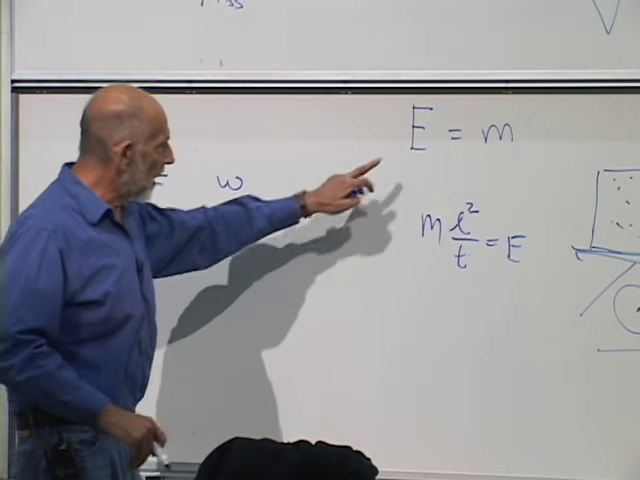
\includegraphics[width=0.72\textwidth]{lecture_01_figure_05.png}
\caption{在 \(c=1\) 的單位制中，靜止的有質量物體，其靜止能量為 \(E=m\)。}
\lectureframe{01:25:40}
\end{figure}

這些公式看起來相似，意義卻不同。在 \(E_{\mathrm{rest}}=m\) 中，\(E\) 是有質量物體的靜止能量。光子沒有質量，也無法靜止，因此它的能量不是靜止能量。關係式 \(E_\gamma=\omega\) 描述的是運動中的無質量量子所具有的能量。

\begin{classroomqa}
\lecturetimestamp{01:26:07}
\audiencequestion{既然靜止總是相對於某個參考物而言，而且實驗室本身也不是絕對靜止的，\emph{靜止}究竟是什麼意思？}
\lecturerresponse{靜止是相對於所選參考系來定義的。如果杯子相對於實驗室靜止，那麼在實驗室參考系中，當 \(c=1\) 時，它的能量就是它的質量，不含整體運動所造成的動能。另一位從杯子旁經過的觀察者，則會認為杯子也具有動能。不同觀察者通常會為同一物體或光子測得不同的能量；能量取決於參考系，這並不需要假設存在絕對靜止。}
\end{classroomqa}

現在可以重新檢視角頻率的約定。寫成 \(E_\gamma=\hbar\omega\) 很簡潔，但先前引入 \(\omega=2\pi f\) 時，還多出了一個 \(2\pi\) 因子。

\begin{classroomqa}
\lecturetimestamp{01:28:13}
\audiencequestion{為什麼要使用以弧度每秒為單位的角頻率 \(\omega\)，而不用看似更簡單的每秒完整週期數？}
\lecturerresponse{這個選擇部分出於歷史因素；至於數學上的理由，答案並非顯而易見，而是取決於實際使用。這裡提供的答案仍屬暫定：分別用 \(f\) 和 \(\omega\) 寫出相關方程式，再看看哪種約定留下的 \(2\pi\) 因子較少。不論如何選擇，\(2\pi\) 因子都不可能在所有地方消失。有人也提出，這可能與複指數記號有關，但這裡不再深入討論。}
\end{classroomqa}

\begin{classroomqa}
\lecturetimestamp{01:29:51}
\audiencequestion{能否將兩個粒子加速，直到它們之間的重力作用變得重要？}
\lecturerresponse{原則上可以。實際上，目前的加速器離這個範圍還非常遙遠。答案也取決於「粒子」的定義：宏觀的受重力物體並非這裡所討論的基本粒子。}
\end{classroomqa}

\begin{classroomqa}
\lecturetimestamp{01:30:27}
\audiencequestion{什麼可以作為正電子的來源？}
\lecturerresponse{高能碰撞可以產生正電子。有些核過程與衰變也會產生正電子。}
\end{classroomqa}

\begin{classroomqa}
\lecturetimestamp{01:30:53}
\audiencequestion{這裡使用的自然單位是普朗克時間和普朗克距離嗎？}
\lecturerresponse{不是。當 \(G\)、\(c\) 和 \(\hbar\) 都設為一時，便得到普朗克單位。由此定義的普朗克長度遠小於一般粒子物理涉及的長度尺度，因此不適合作為這裡的量尺。當重力、量子力學和相對論都同時重要時，例如在黑洞物理、宇宙學或量子重力中，這類單位才自然合用。若重力可以忽略，只將 \(c\) 和 \(\hbar\) 設為一會更實用。}
\end{classroomqa}

\section{動量、光與解析度}

接下來要介紹的基本概念是動量。物體靜止時沒有動量，儘管它具有非零的靜止能量 \(mc^2\)。物體一旦運動，通常就會帶有動量。動量和能量一樣，在碰撞中守恆：兩個物體碰撞前後，總向量動量相同。凡是受守恆定律約束的物理量，都值得特別留意。

動量是向量，方向沿著運動方向。對非相對論性物體，
\begin{equation}
\mathbf p=m\mathbf v.
\end{equation}
這不是一般的相對論公式，不能直接用於光。

不過，光也攜帶動量和能量。一般光所產生的推力極小，動量很難察覺；但強烈的雷射脈衝可以傳遞相當大的衝量。例如，利佛摩爾的大型雷射可以利用輻射攜帶的動量，將物質向內推。

考慮一個準直程度足夠高、光線幾乎沿著單一軸向傳播的脈衝。真實光束可能有一定的角度散布，各部分沿著略有差異的方向傳播；但對理想的準直光束而言，動量方向沿著光束，大小為
\begin{equation}
p=\frac{E}{c},
\qquad\text{or equivalently}\qquad
E=cp.
\end{equation}
這裡將此關係視為相對論中的一項事實，而不加以證明。以下的量綱檢查只能確認它的單位與一般動量的單位相符：
\begin{equation}
\left[\frac{E}{c}\right]
=
\frac{M L^2 T^{-2}}{L T^{-1}}
=
M L T^{-1}
=
[m v]
=
[p].
\end{equation}
這項量綱比較並未賦予光靜止質量。光子的質量為零；它之所以具有動量，是因為它攜帶能量，並以 \(c\) 運動。

\(\mathbf p\) 的方向就是傳播方向。它的大小通常難以測量，因為 \(c\) 出現在分母。光束可以輕易透過加熱或蒸發物質，展現所攜帶的能量；相較之下，它造成的機械推力小得多。不過，只要強度夠大，這股推力也可以變得很大。

對單一光子而言，
\begin{align}
p_\gamma
&=\frac{E_\gamma}{c}\\
&=\frac{\hbar\omega}{c}.
\end{align}
要改用波長表示，必須仔細回到波的關係式。由於
\begin{equation}
f\lambda=c,
\qquad
\omega=2\pi f,
\end{equation}
正確的關係式是
\begin{equation}
\omega\lambda=2\pi c,
\qquad
\omega=\frac{2\pi c}{\lambda}.
\end{equation}
若沒有先寫出定義，\(2\pi\) 這個因子很容易顛倒。重新從 \(f\lambda=c\) 和 \(f=\omega/(2\pi)\) 出發，就能釐清：
\begin{equation}
\frac{\omega}{2\pi}\lambda=c
\quad\Longrightarrow\quad
\omega\lambda=2\pi c.
\end{equation}
代入後得到
\begin{align}
p_\gamma
&=\frac{\hbar}{c}\frac{2\pi c}{\lambda}\\
&=\frac{2\pi\hbar}{\lambda}\\
&=\frac{h}{\lambda}.
\end{align}

\begin{classroomqa}
\lecturetimestamp{01:42:38}
\audiencequestion{\(2\pi\hbar\)等於 \(h\) 嗎？}
\lecturerresponse{是的。依定義，\(h=2\pi\hbar\)，所以 \(p_\gamma=2\pi\hbar/\lambda\) 與 \(p_\gamma=h/\lambda\) 相同。無論選用哪種頻率約定，某處都會重新出現 \(2\pi\) 因子。}
\end{classroomqa}

波長越短，光子的動量越大。無線電波光子的波長很長，動量極小；伽馬射線光子的波長很短，造成的衝擊大得多。單一光子帶來的宏觀衝量仍然很小，但其動量遠大於無線電波光子。它的能量也比較大，因為 \(E_\gamma=cp_\gamma\)。

這個關係說明了為什麼要觀察越小的物體，就需要越大型的機器。若用遠長於人頭的波長拍照，影像只會模糊一片。要分辨五官，波長必須短於頭部尺寸；要看清一根頭髮，波長必須與髮絲的粗細相當或更短；要解析原子的結構，探測波長不能大於原子：
\begin{equation}
\lambda_{\mathrm{probe}}\lesssim
\text{size of the structure to be resolved}.
\end{equation}
因此，結構越小，所需的波長越短；波長越短，所需的動量和能量就越大。探測粒子不一定是光子；其他種類的高能粒子也遵循相同的波長與動量之間的量子關係。要產生這些粒子，必須用加速器將越來越多的能量傳給每個粒子。\(p_\gamma=h/\lambda\) 和 \(E_\gamma=\hbar\omega\) 這兩個關係式串起了整個論證：提高探測能量會增加動量並縮短波長。

近一個世紀以來，粒子物理學反覆呈現相同的脈絡：能量越高、動量越大、波長越短，空間解析度也越精細。

\begin{classroomqa}
\lecturetimestamp{01:46:57}
\audiencequestion{波長在理論上有沒有下限？}
\lecturerresponse{可能有。在普朗克長度附近，預期會出現新的現象，但這個答案仍屬暫定。即使空間解析度真的在那個尺度觸及下限，它仍比大型強子對撞機目前探測的距離小約十七個數量級；因此，現今實驗距離那個尺度還非常遙遠。}
\end{classroomqa}

沿著同一套推理，可以粗略看出加速器的尺度與它能解析的尺度之間的關係。

\begin{classroomqa}
\lecturetimestamp{01:48:02}
\audiencequestion{波長，或者說所解析的尺寸，是否大致與加速器的尺寸成反比？}
\lecturerresponse{大致如此，前提是加速粒子所用的最大電場，以及引導粒子所用的磁場，都受限於現有設備。加速梯度表示每單位長度所增加的能量。對於長度為 \(L\)、加速梯度 \(\mathcal G\) 大致固定的直線加速器，
\[
E_{\mathrm{beam}}\sim \mathcal G L.
\]
在超相對論能量下，可解析的波長與能量成反比，因此加長直線加速器，大致會以相應的反比因子提升解析度。這只是啟發式的尺度關係，並非精確定律。環形加速器可以讓粒子反覆通過同一設備，但帶電粒子在彎轉時會輻射並損失能量。}
\end{classroomqa}

\begin{classroomqa}
\lecturetimestamp{01:49:47}
\audiencequestion{要達到普朗克長度，加速器得有多大？}
\lecturerresponse{按照這個粗略的尺度關係，加速器必須比 CERN 的加速器長約十七個數量級。這還不到宇宙的尺度，但大致相當於星系的尺度。}
\end{classroomqa}

\begin{classroomqa}
\lecturetimestamp{01:50:09}
\audiencequestion{最高能量宇宙射線的能量，與對撞機能量相比如何？}
\lecturerresponse{單一宇宙射線的能量可以遠高於實驗室能量。為了作數值比較，取一個實驗室能量約為 \(10^{21}\,\mathrm{eV}=10^{12}\,\mathrm{GeV}\) 的極高能宇宙射線。然而，宇宙射線撞擊的是在實驗室中靜止的靶；對撞機則讓兩束高能粒子束迎頭碰撞。更重要的是，進行有用的實驗需要足夠的通量，也就是大量粒子和許多受控良好的碰撞。單一宇宙射線可能打不中相關的靶，或只產生一個難以推知任何結果的事件。一項刻意誇大的石油當量估算指出，要讓一座有用的星系尺度加速器運轉，每秒所需的石油供應量約為一百兆桶。這個估算是要說明，取得足夠的碰撞統計量，至少會和加速器的長度一樣，構成嚴重障礙。}
\end{classroomqa}

\editorialnote{來源中的石油當量估算前後不一致：先提出一個數值，接著又說約為每秒 \(10^{14}\) 桶；後來再次敘述時，則給出每秒 \(10^{11}\) 桶。這裡保留兩種數量級，沒有逕自將它們調整成一致。}

這些都是實際的距離尺度，不只是形式上的尺度。實際難題在於，如何不建造星系尺度的加速器，也不提供其荒誕的所需功率，就能探測這些尺度。

\begin{classroomqa}
\lecturetimestamp{01:52:55}
\audiencequestion{應如何將 LHC 的能量與能量為 \(10^{12}\,\mathrm{GeV}\) 的宇宙射線相比？}
\lecturerresponse{對於實驗室能量為 \(E_{\mathrm{lab}}\)、撞擊質量為 \(m_{\mathrm{target}}\) 的靜止靶的超相對論性入射粒子，質心能量的尺度關係為
\[
E_{\mathrm{cm}}\simeq
\sqrt{2m_{\mathrm{target}}c^2E_{\mathrm{lab}}}.
\]
\editorialnote{這裡列出的固定靶公式，明確呈現了問答中所述的平方根尺度關係。}
因此，在靶的質量固定時，有效碰撞能量只會隨入射粒子能量的平方根增加。所以，能量為 \(10^{12}\,\mathrm{GeV}\) 的宇宙射線，約相當於兩束迎頭相撞、每束能量約為 \(10^6\,\mathrm{GeV}\) 的粒子束，而不是每束 \(10^{12}\,\mathrm{GeV}\)。宇宙射線的能量仍可能超過地面對撞機，但其通量極低，無法用於系統性的受控實驗。}
\end{classroomqa}
\chapter{波、量子化模式與產生算符}

\section{波、場與複指數}

量子場論是粒子物理學的基本工具。在初步介紹量子場之前，先整理連結波與粒子的數學事實很有幫助。波本身就是一種場的組態：場在空間中逐點變化，而波則是場值振盪並傳播的一種組態。量子力學提供了這類波與粒子之間的連結。

這裡假定讀者已具備量子力學與狹義相對論的背景知識。本節的直接目的，是回顧粒子物理學所需的部分內容，而非取代這兩門學科的課程。

指數函數的特徵是按比例增長。若
\begin{equation}
f(x)=e^{\alpha x},
\end{equation}
則
\begin{equation}
\frac{df}{dx}=\alpha f.
\end{equation}
在很小的區間內，增量與原有的量成正比。培養皿中的族群增長是個熟悉的例子：個體越多，可繁殖的個體就越多，因此增長率與族群本身成正比。將 \(e^{\alpha x}\) 乘上一個整體常數，並不會改變這項定義性質。

正弦與餘弦會振盪，而不會增長。它們是同一條曲線相差四分之一週期的平移，微分後則會彼此轉換：
\begin{align}
\frac{d}{dx}\sin(kx)&=k\cos(kx),\\
\frac{d}{dx}\cos(kx)&=-k\sin(kx).
\end{align}
單獨來看，兩個函數都不是指數函數，因為其中一個函數的導數與另一個函數成正比。不過，複數線性組合確實具有指數函數的性質。令 \(i^2=-1\)，
\begin{align}
\frac{d}{dx}\bigl(\cos(kx)+i\sin(kx)\bigr)
&=-k\sin(kx)+ik\cos(kx)\\
&=ik\bigl(\cos(kx)+i\sin(kx)\bigr).
\end{align}
因此
\begin{equation}
e^{ikx}=\cos(kx)+i\sin(kx).
\end{equation}
這個恆等式一再出現，因為正弦和餘弦描述了波動式的振盪。當 \(x\) 是空間座標時，函數會隨空間振盪；當自變數是時間時，函數則會隨時間振盪。

\section{頻率、波長與光子動量}

普通頻率 \(f\) 是每秒完成的週期數。一個週期就是一次完整的振盪。角頻率以每秒幾弧度來量度相同的運動：
\begin{equation}
\omega=2\pi f.
\end{equation}
這兩種記法描述的是同一個頻率。計算時有時會在兩者之間轉換，以免出現不必要的 \(2\pi\) 因子；不過，這些因子終究不會完全消失。

波長 \(\lambda\) 是一個完整空間週期所占的距離。若波以速率 \(v\) 傳播，則每個週期的距離乘上每秒的週期數，便是傳播速率：
\begin{equation}
\lambda f=v.
\end{equation}
對真空中的光而言，\(v=c\)，因此
\begin{equation}
\lambda f=c.
\end{equation}
聲波的等式右側是聲速；水波則是相應的水波速率。因此，出現 \(c\) 是光的性質，並非所有波都適用的定義。

量子力學以兩種記法引入普朗克常數：
\begin{equation}
\hbar=\frac{h}{2\pi}.
\end{equation}
從 \(h\) 改用 \(\hbar\)，只不過是把 \(2\pi\) 因子從一個方程式移到另一個方程式。

有量綱常數的數值取決於表示它們時所用的單位。公尺、秒和公斤是符合人類尺度的慣用單位，方便描述日常的長度與時間。以手臂長度為基準的傳統單位，曾適用於布料或繩索；無論公尺的歷史沿革究竟如何，都沒有基本原理會特別選定這種符合人類尺度的單位。在 SI 單位制中，
\begin{equation}
\begin{aligned}
h &\simeq 6.6\times10^{-34}\ \mathrm{J\,s},
&\hbar &\simeq 1.1\times10^{-34}\ \mathrm{J\,s},\\
c &\simeq 3\times10^8\ \mathrm{m\,s^{-1}}.
\end{aligned}
\end{equation}
這些數值要表達的是它們在慣用單位下的尺度：普朗克常數極小，而光速極大。

一個模式中的單一量子具有能量
\begin{equation}
E_{\text{one quantum}}=\hbar\omega=hf.
\end{equation}
這是單一光子的能量，並非任意經典電磁波的總能量。可見光的頻率約為每秒 \(10^{15}\) 個週期，因此典型光學光子的能量約為
\begin{equation}
E_\gamma\sim 10^{-19}\ \mathrm{J}.
\end{equation}
光學振盪即使如此迅速，每個量子的能量仍極小，因為 \(h\) 非常小。因此，宏觀尺度的光能包含數量極其龐大的光子。

能量和動量特別值得注意，因為兩者都是守恆量。它們是有用的帳目：進入某個過程的總能量與總動量，必須和離開該過程的總能量與總動量相平衡。動量是向量，方向與運動方向相同。對於運動速度遠低於光速的粒子，
\begin{equation}
\vec p=m\vec v.
\end{equation}

現在考慮沿單一方向準直傳播、而非向許多方向散開的電磁輻射。它的動量沿著光束方向。非相對論公式不能用於光子，因為 \(m\) 表示靜止質量，而光子的靜止質量為零。儘管如此，有個實用的量綱助記法：若 \emph{不恰當地}把 \(E/c^2\) 當成質量賦予光子，再代入 \(v=c\)，就會得到
\begin{equation}
mv\longrightarrow \frac{E}{c^2}c=\frac{E}{c}.
\end{equation}
這個做法碰巧得到正確答案，量綱也正確，但不能據此合理地論證光子具有靜止質量 \(E/c^2\)。準直輻射的正確相對論敘述是
\begin{equation}
|\vec p|=\frac{E}{c}.
\end{equation}
這個方程式給出動量的大小；動量方向則與輻射傳播方向相同。

對單一光子而言，
\begin{align}
|\vec p_\gamma|
&=\frac{E_\gamma}{c}
=\frac{hf}{c}.
\end{align}
對光而言，
\begin{equation}
\lambda f=c,
\qquad
\frac{f}{c}=\frac{1}{\lambda},
\end{equation}
因此
\begin{equation}
|\vec p_\gamma|=\frac{hf}{c}=\frac{h}{\lambda}.
\end{equation}

\begin{figure}[t]
\centering
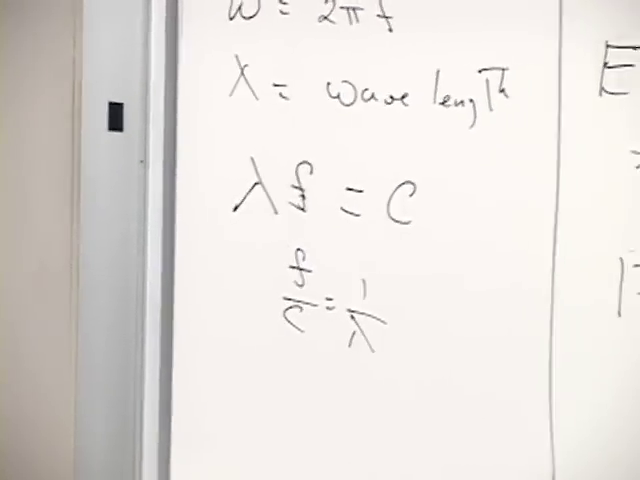
\includegraphics[width=0.56\textwidth]{lecture_02_figure_02.png}
\caption{對光而言，\(\lambda f=c\)與\(f/c=1/\lambda\)，便可得到\(|\vec p_\gamma|=h/\lambda\)。}
\lectureframe{00:21:39}
\end{figure}

波長越短，光子動量越大。這是粒子物理學中最重要的量子事實之一。要研究微小物體，需要以短波長作為探測；短波長所付出的代價，就是較大的動量。

\begin{classroomqa}
\lecturetimestamp{00:22:23}
\audiencequestion{\(E=\hbar\omega\)是基本原理，還是可以從更深層的原理推導出來？}
\lecturerresponse{這個結果可由諧振子的量子力學推導而得。這裡會直接使用此結果，不再重複證明；下文建立的振子描述，會說明它更深層的背景。}
\end{classroomqa}


\section{波的振幅與光子數}

\begin{classroomqa}
\lecturetimestamp{00:23:10}
\audiencequestion{以光子的語言來說，波的振幅代表什麼？}
\lecturerresponse{比較兩個波長和頻率相同、但振幅不同的波，例如 \(\sin(kx)\) 和 \(A\sin(kx)\)。在經典物理中，固定區域內的能量與振幅平方成正比。在量子力學中，含有 \(n\) 個光子的模式具有能量 \(n\hbar\omega\)。因此，在頻率、區域和正規化方式都固定時，振幅的量級會隨 \(\sqrt n\) 增長。}
\end{classroomqa}

兩個波的振盪型態完全相同，只是一個比另一個強。\footnote{示意圖參照 00 至 23 的波形比較：47--00至24：28。}

\begin{figure}[t]
\centering
\begin{tikzpicture}[x=1cm,y=0.65cm]
\draw[->] (-0.4,0) -- (6.8,0);
\draw[->] (-0.4,-2.1) -- (6.8,-2.1);
\draw[thick] plot[domain=0:6.2,samples=120] (\x,{0.45*sin(\x r)});
\draw[thick] plot[domain=0:6.2,samples=120] (\x,{-2.1+1.15*sin(\x r)});
\draw (6.2,0.55) node[right]{small amplitude};
\draw (6.2,-0.75) node[right]{large amplitude};
\end{tikzpicture}
\caption{波長與頻率相同、振幅不同的波。}
\end{figure}

對固定的波量而言，
\begin{equation}
E_{\text{wave}}\propto A^2.
\end{equation}
對電磁波來說，這就是熟知的場能與場強平方成正比。如果同一個模式含有 \(n\) 個光子，那麼
\begin{equation}
E_{\text{wave}}=n\hbar\omega.
\end{equation}
因此，在模式、頻率、正規化方式和區域都固定時，
\begin{equation}
A^2\propto n\hbar\omega,
\qquad
A\propto\sqrt n\quad\text{at fixed }\omega.
\end{equation}
這裡並未主張任何精確的正規化關係。波的涵蓋範圍很重要：將原本均勻的波長度加倍，會改變總能量，卻不會改變局部振幅。因此，這個正比關係應理解為適用於固定區域，例如一個波長。

此外，量子力學還有一項特有的限制：振幅和相位不能同時具有精確的經典值。因此，若問題 ``單一光子的振幅是多少？'' 要求的是完全確定的經典場，便沒有明確答案。不過，令 \(n=1\) 仍可得到合理的量級估計。

\begin{classroomqa}
\lecturetimestamp{00:28:25}
\audiencequestion{電磁波圖中的垂直位移代表光子在空間中的位置嗎？}
\lecturerresponse{不代表。傳播軸是空間座標，而垂直座標表示電場或磁場的值。動量沿傳播軸方向，不是沿圖中場振幅的方向。}
\end{classroomqa}

波可以沿任意空間方向傳播，但熟悉的正弦波圖只把水平軸當作空間座標。圖中另一個方向表示場強。

\begin{classroomqa}
\lecturetimestamp{00:29:37}
\audiencequestion{所說的光子數，是在一個波長或一個週期內計算的嗎？}
\lecturerresponse{可以選定一個固定區域，例如一個波長。這就是為什麼此處只有正比關係：總能量和光子數也取決於涵蓋了多少波。在振幅相同的情況下，涵蓋兩個、三個或四個波長，能量就相應增加。}
\end{classroomqa}

\begin{classroomqa}
\lecturetimestamp{00:30:17}
\audiencequestion{單一光子的振幅沒有意義嗎？}
\lecturerresponse{只有在令 \(n=1\) 後，將其視為量級估計，才有意義。對電磁模式而言，電場和磁場資訊的作用類似於共軛的位置與動量資訊，因此量子不確定性限制了經典振幅能指定得多精確。量級關係仍然有用。}
\end{classroomqa}

這些問題已經引向量子場論；在量子場論中，場變數與粒子數之間的關係可以精確表述。目前只需掌握這些正比關係。

\section{一般量子關係與慢速物質波}

有些為光子引入的公式適用範圍更廣，有些則不然。在討論電子之前，值得先釐清各公式的適用範圍。

\begin{figure}[t]
\centering
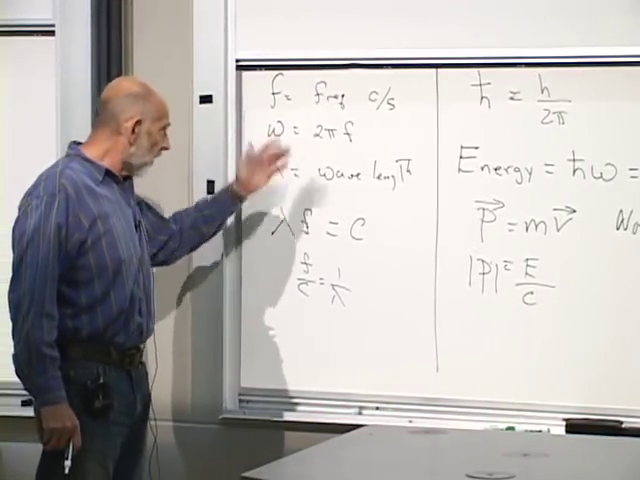
\includegraphics[width=0.82\textwidth]{lecture_02_figure_03.png}
\caption{波的定義，以及光子與非相對論動量關係的適用範圍比較。}
\lectureframe{00:31:52}
\end{figure}

\(f\)、\(\omega=2\pi f\)和\(\lambda\)的定義普遍適用。在此處的討論中，量子關係
\begin{equation}
E=\hbar\omega=hf
\end{equation}
也普遍適用。相較之下，含有 \(c\) 的公式，例如 \(\lambda f=c\) 和 \(|\vec p|=E/c\)，適用於以光速傳播的波。公式 \(\vec p=m\vec v\) 則適用於運動速度遠低於光速的粒子。介於這兩種情形之間的相對論運動，需要用到目前還不必介紹的插值公式。

動量--波長關係在光子的例子中仍然成立：
\begin{equation}
p=\frac{h}{\lambda}.
\end{equation}
這裡的 \(p\) 表示大小，並假設 \(\lambda\) 是正的波長；方向可以另外指定。

\begin{figure}[t]
\centering
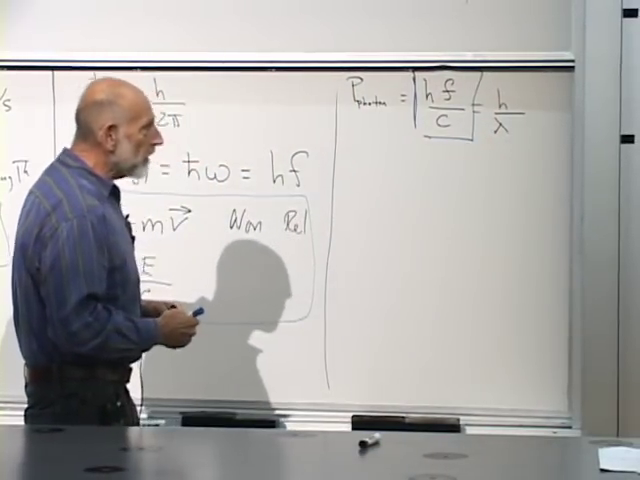
\includegraphics[width=0.74\textwidth]{lecture_02_figure_04.png}
\caption{光子動量 \(|\vec p_\gamma|=hf/c=h/\lambda\)，由此得到一般的德布羅意關係。}
\lectureframe{00:33:32}
\end{figure}

電子、原子核，甚至保齡球都可以與波相聯繫。電子干涉就是這個事實的一種表現。將電子波寫成 \(\psi\)。對於緩慢運動的電子，什麼關係取代了 \(\lambda f=c\)？缺少的關鍵是能量與動量之間的非相對論關係。

從動能和動量開始：
\begin{align}
E&=\frac12 mv^2,\\
p&=mv,
\qquad
v=\frac{p}{m}.
\end{align}
將最後一個關係代入第一個，得到
\begin{align}
E
&=\frac12m\left(\frac{p}{m}\right)^2\\
&=\frac{p^2}{2m}.
\end{align}
質量在 \(\frac12 mv^2\) 中位於分子，在 \(p^2/(2m)\) 中則位於分母。這兩處很容易混淆，也值得重新推導一次。

現在使用一般的量子關係
\begin{equation}
E=hf,
\qquad
p=\frac{h}{\lambda}.
\end{equation}
對單一慢速粒子而言，
\begin{align}
hf
&=\frac{p^2}{2m}\\
&=\frac{1}{2m}\left(\frac{h}{\lambda}\right)^2\\
&=\frac{h^2}{2m\lambda^2}.
\end{align}
兩邊除以 \(h\)，得到
\begin{equation}
f=\frac{h}{2m\lambda^2}.
\end{equation}

\begin{figure}[t]
\centering
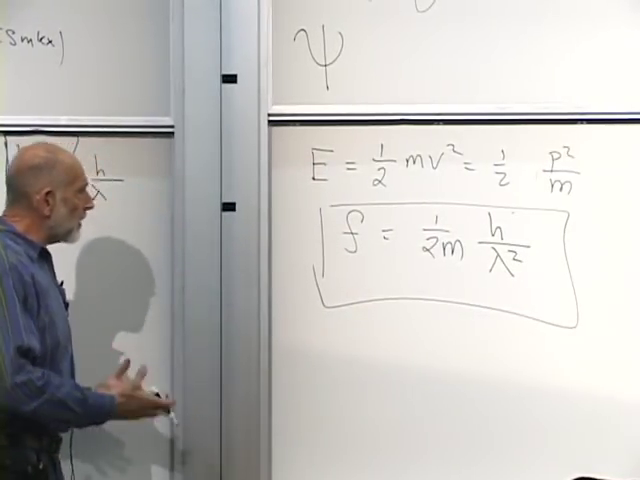
\includegraphics[width=0.64\textwidth]{lecture_02_figure_05.png}
\caption{對慢速粒子而言，\(E=p^2/(2m)\)和\(p=h/\lambda\)可得\(f=h/(2m\lambda^2)\)。}
\lectureframe{00:37:47}
\end{figure}

對光而言，
\begin{equation}
f\propto\frac{1}{\lambda},
\end{equation}
對慢速物質而言，
\begin{equation}
f\propto\frac{1}{\lambda^2}.
\end{equation}
不必孤立地記住第二個關係，隨時都可以由 \(E=p^2/(2m)\)、\(E=hf\) 和 \(p=h/\lambda\) 推導出來。它給出原子中緩慢運動的電子所對應的 Schr\"odinger 波頻率。

\begin{classroomqa}
\lecturetimestamp{00:38:35}
\audiencequestion{非相對論的頻率--波長關係也適用於電子以外的粒子嗎？}
\lecturerresponse{是的。它適用於任何運動速度遠低於光速的粒子。慢速極限與光速極限之間的相對論插值，是另一個主題。}
\end{classroomqa}

\begin{classroomqa}
\lecturetimestamp{00:38:55}
\audiencequestion{哪一個關係適用於中微子？}
\lecturerresponse{要看中微子的速度。自然界中遇到的大多數中微子都以非常接近光速的速度運動，因此光速情形的關係是很好的近似。若中微子的速度遠低於光速，則適用非相對論關係。}
\end{classroomqa}

\editorialnote{中微子問題之後，緊接著有一段簡短的聽眾交流，談到振幅、量子和電子波長的差異，但內容損壞嚴重，無法確實還原。仍可辨認的回答表示，會稍後再討論不同波長的振幅與量子之間的一般關係。}

\begin{classroomqa}
\lecturetimestamp{00:39:56}
\audiencequestion{來自 \(20\,\mathrm{keV}\) 加速器的電子是慢速粒子，還是相對論性粒子？}
\lecturerresponse{這裡將它視為慢速粒子。在 \(c=1\) 單位制中，質量、能量和動量可以用相同單位表示。電子的靜能量級約為 \(0.5\,\mathrm{MeV}\)，而 \(20\,\mathrm{keV}\) 小得多。等價地說，非相對論動量判準是 \(p\ll mc\)。}
\end{classroomqa}

此例中的能量比較為
\begin{equation}
K=20\,\mathrm{keV}\ll m_ec^2\simeq0.5\,\mathrm{MeV}.
\end{equation}
\editorialnote{00處的原文段落：39：56--00：41：40先將 \(20\,\mathrm{keV}\) 作為加速器能量提出，接著以動量和靜質量的比較來表述相對論判準。分別寫出動能判準和動量判準，可以避免把引述的能量等同於動量，同時保留原文所述的非相對論結論。}

\section{相速度、群速度與色散}

\begin{classroomqa}
\lecturetimestamp{00:41:46}
\audiencequestion{頻率乘以波長，能用來求得電子波的速度嗎？}
\lecturerresponse{這樣得到的是相速度，不是電子本身的速度。局域化波包有兩種速度：描述內部波峰和波谷運動的相速度，以及描述包絡運動的群速度。群速度對應於粒子的運動速度。}
\end{classroomqa}

波包在局部看起來像正弦或餘弦波，但受到包絡限制。波包移動時，包絡和其中的波峰不一定以相同速度前進。\footnote{示意圖參照 00 至 42 的波包討論：34--00至44：11。}

\begin{figure}[t]
\centering
\begin{tikzpicture}[x=0.75cm,y=0.8cm]
\draw[->] (-0.5,0) -- (12.8,0);
\draw[thick] plot[domain=0:12,samples=140] (\x,{1.10*exp(-0.20*(\x-6)^2)});
\draw[thick] plot[domain=0:12,samples=140] (\x,{-1.10*exp(-0.20*(\x-6)^2)});
\draw[thick] plot[domain=0:12,samples=240] (\x,{1.10*exp(-0.20*(\x-6)^2)*sin(6*\x r)});
\draw[->] (4.1,1.45) -- (7.5,1.45);
\draw (5.8,1.8) node{group motion};
\draw[->] (7.0,-1.55) -- (8.3,-1.55);
\draw (8.7,-1.55) node[right]{phase motion};
\end{tikzpicture}
\caption{局域化波包的包絡和內部相位通常以不同速度移動。}
\end{figure}

相速度是單色分量中波峰、波谷和其他固定相位的移動速度。對非相對論性色散關係而言，
\begin{equation}
v_\phi=f\lambda=\frac{h}{2m\lambda}.
\end{equation}
相速度取決於波長。因此，不同波長的分量具有不同的相速度，波峰會在波包內移動，而波包也會發生色散。群速度是整個波包的移動速度，也就是對應於粒子的速度。

有一個簡單的特例：如果所有波長的分量都以相同速度移動，相速度和群速度便相同。真空中的光就具有這項性質：所有波長都以 \(c\) 傳播。慢速粒子的關係則不同；其中的 \(f\lambda\) 會隨 \(\lambda\) 改變。

方程式
\begin{equation}
f=\frac{h}{2m\lambda^2}
\end{equation}
稍加改寫後，就是自由 Schr\"odinger 方程式。頻率決定平面波的時間依賴性，波長決定它的空間依賴性，而 Schr\"odinger 方程式則連結兩者。反過來說，將頻率和波長皆確定的波代入自由 Schr\"odinger 方程式，就會得到這個色散關係。

\begin{classroomqa}
\lecturetimestamp{00:47:02}
\audiencequestion{相速度可以超過光速嗎？}
\lecturerresponse{可以。相速度不會傳遞資訊。資訊和局域化波包以群速度傳播，因此相速度超光速並不代表可以超光速傳遞訊號。}
\end{classroomqa}

\section{有限空間與離散動量}

我們最終要探討的是無限空間中的波，但從有限系統開始較為穩妥。電腦無法直接儲存或操作無限。首先要為有限系統建立方程式，之後再取系統大小任意增大的極限。這種做法在量子力學、量子場論和粒子物理學中都很有用。

從一維空間開始，不會失去任何本質內容。波可以存在於小提琴弦、被抖動的繩子，或抽象的一維世界中。最直觀的有限系統，是一段長度為 \(L\)、兩端會反射的線段。波傳到端點後反射，再傳回來。這種反射邊界條件完全合理，但有個缺點：波系統內部的動量不守恆。向右傳播的波帶有向右的動量；反射後則帶有向左的動量。邊界提供了衝量，並吸收動量差。

端點反射造成動量反向，可以用示意圖表示。\footnote{示意圖參照 00 至 49 的反射邊界論證：24--00至51：08。}

\begin{figure}[t]
\centering
\begin{tikzpicture}[x=1cm,y=1cm]
\draw[thick] (0,0) -- (7,0);
\draw[very thick] (0,-0.45) -- (0,0.45);
\draw[very thick] (7,-0.45) -- (7,0.45);
\draw[->,thick] (1.0,0.35) -- (5.8,0.35) node[midway,above]{\(p>0\)};
\draw[->,thick] (5.8,-0.35) -- (1.0,-0.35) node[midway,below]{\(p<0\)};
\draw (3.5,-0.85) node{\(L\)};
\end{tikzpicture}
\caption{有限線段兩端的反射會使行波的動量反向。}
\end{figure}

還有另一種讓系統有限、同時保留動量守恆的方法：將線段的兩個端點視為同一點。可以把結果畫成一個圓，但不需要真的有一個嵌在二維空間中的圓。數學上的意思很簡單：座標具有週期性，走過總長度 \(L\) 後，就會回到同一點。

\begin{figure}[t]
\centering
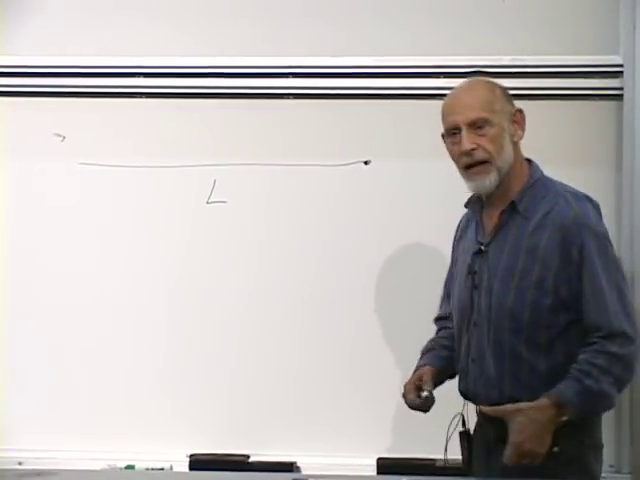
\includegraphics[width=0.72\textwidth]{lecture_02_figure_06.png}
\caption{總長度為 \(L\) 的一維路徑，用以介紹週期性識別。}
\lectureframe{00:51:21}
\end{figure}

下方示意圖明確呈現端點識別。\footnote{示意圖參照 00 至 51 的週期性識別論證：09--00至52：37。}

\begin{figure}[t]
\centering
\begin{tikzpicture}[x=1cm,y=1cm]
\draw[thick] (0,0) -- (7,0);
\fill (0,0) circle (1.5pt);
\fill (7,0) circle (1.5pt);
\draw[->,thick] (1.0,0.35) -- (6.0,0.35);
\draw (3.5,-0.35) node{\(L\)};
\draw[->,bend left=45] (7,0.08) to (0,0.08);
\draw (3.5,1.2) node{identified endpoints};
\end{tikzpicture}
\caption{將長度為 \(L\) 的路徑兩端識別後形成的週期性一維空間。}
\end{figure}

向右移動的波接著抵達圖示端點，從起點重新出現，並繼續向右移動。向左移動的波也會繼續向左。由於沒有特定端點讓波反射，動量便不會反向。週期性空間使體積有限且保留動量，但也帶來一項重要結果：允許的動量是離散的。

總長度內必須容納整數個波長。對非定值模式而言，
\begin{equation}
\lambda_{|N|}=\frac{L}{|N|},
\qquad |N|=1,2,3,\ldots .
\end{equation}
因此波長的大小可以是 \(L\)、\(L/2\)、\(L/3\) 等。像 \(L/\sqrt{2}\) 這樣的選擇便不符合條件：波繞行一圈後會以錯誤的相位返回，無法與起始值相接。

利用 \(p=h/\lambda\)，第 \(|N|\) 個非定值模式的動量大小為
\begin{equation}
|p_N|=\frac{|N|h}{L}.
\end{equation}
若要毫無歧義地涵蓋兩個傳播方向和定值模式，將模式標記設為正負皆可會較方便：
\begin{equation}
p_N=\frac{Nh}{L},
\qquad N=0,\pm1,\pm2,\ldots .
\end{equation}
\(N\) 為正或負，代表相反的傳播方向。\(N=0\) 模式為定值模式，動量為零；它沒有有限波長可代入 \(h/\lambda\)。因此，基本動量間距為 \(h/L\)。

對宏觀的 \(L\) 而言，\(h\) 和 \(1/L\) 都使動量間距極小，因此允許值非常密集，看起來幾乎連續。然而，受限於圓形金屬線上運動的珠子，仍恰好具有這種離散譜。

\begin{classroomqa}
\lecturetimestamp{00:58:27}
\audiencequestion{量子化的是波的總動量，還是與單一週期相關的動量？}
\lecturerresponse{這項敘述適用於每個量子的動量。每個量子的動量都必須是允許的離散值之一。因此，任意一群量子的總動量也會是基本單位 \(h/L\) 的整數倍。}
\end{classroomqa}

\begin{classroomqa}
\lecturetimestamp{00:59:22}
\audiencequestion{為什麼波繞行一圈後必須回到相同的值？}
\lecturerresponse{識別後的兩個端點是同一個物理位置，因此可觀測的場在該處必須具有相同的值。若兩側不匹配，場在該處就會突然跳變。這種不連續性需要付出很大的能量與動量代價；可容許的場組態必須連續且具有週期性。}
\end{classroomqa}

\begin{classroomqa}
\lecturetimestamp{01:00:09}
\audiencequestion{如果波局域成一個波包，會怎麼樣？}
\lecturerresponse{波包是平面波的傅立葉和，也可以說是正弦波與餘弦波的傅立葉和。在週期性空間中，這個和只能包含允許的離散動量模式。因此，量子化的敘述適用於每個可容許波包的傅立葉分量。}
\end{classroomqa}

\begin{classroomqa}
\lecturetimestamp{01:01:01}
\audiencequestion{週期長度 \(L\) 極小時會出問題嗎？}
\lecturerresponse{隨著 \(L\) 減小，基本動量 \(h/L\) 會變得非常大。在一般微觀尺度下，這不會立即造成矛盾；但若試圖將這個建構推至普朗克長度尺度，預期就需要新的物理。}
\end{classroomqa}

現在將圓形圖像按字面理解：一顆珠子在半徑為 \(r\) 的圓形金屬線上運動，圓周長為 \(L=2\pi r\)。允許的切向動量為
\begin{equation}
p_N=\frac{Nh}{2\pi r}=\frac{N\hbar}{r}.
\end{equation}
對於沿圓形軌道運動的非相對論粒子，角動量為 \(mvr\)。由於在這種情況下 \(p=mv\)，所以角動量就是 \(rp\)。表示式 \(mvr\) 並非相對論情況下的通用形式，因為此時 \(p\) 不再只是 \(mv\)；但動量乘以垂直距離仍是正確的關係。以向量表示，\footnote{講課時先用 \(L\) 表示角動量，隨後發現它與週期長度的符號 \(L\) 相衝突，於是改用了其他符號。這裡一律使用 \(J\)；參見 01：03：40--01：05：21。}
\begin{equation}
\vec J=\vec r\times\vec p,
\end{equation}
切向圓周運動的角動量大小為 \(J=rp\)。因此
\begin{equation}
J_N=rp_N=N\hbar.
\end{equation}
線動量的間距取決於圓的大小，但角動量的單位永遠是 \(\hbar\)。涉及費米子時，整數規則會有例外；這些例外留待之後討論。

接下來要更精確地連結場、粒子和量子。這需要簡短回顧算符與簡諧振子的量子力學。

\section{波模式與量子算符}

接下來的量子力學內容必然較為抽象，目的在於複習。簡諧振子是核心系統，因為波就是一種振盪。在固定位置上，電場、磁場或任何其他波振幅都會隨時間週期性變化；說一個分量具有頻率，就等於說它正在振盪。

一般的波不一定只有一個波長。不同顏色的光可以混合在一起；反過來說，稜鏡也可以把混合光分解成各種組成色，牛頓分解白光就是一例。每個分量都有自己的波長、頻率、振幅、能量和動量。因此，混合波可以分解為具有不同能量和動量的量子。每個波長決定一個頻率，而每個定頻分量的行為都像一個振子。這就是為什麼場的自然基本單元是簡諧振子，而不是任意的量子系統。

量子可觀測量以算符表示。算符可以相加、相乘；但與普通數不同，算符乘積不一定與相乘順序無關。設\(A\)和\(B\)代表系統的兩種性質，各自都可能單獨測量。例如，\(A\)可能代表電場，\(B\)可能代表磁場。若測得的數值是普通數\(a\)和\(b\)，則
\begin{equation}
ab=ba.
\end{equation}
它們的數值乘積不可能因相乘順序而異。然而在量子力學中，相應的算符卻可能滿足\(AB-BA\neq0\)。

乍看之下，這似乎說不通。如果測量電場得到一個數，測量磁場得到另一個數，那麼這兩個數相乘，無論順序如何，結果都必須相同。解決之道在於：若算符乘積會因順序而異，這兩個量就不能同時測量。測量其中一個的實驗會干擾另一個量的測量。這並不矛盾，因為這兩個數值無法同時取得。

若兩個量可以同時測量，測得的數值就是普通數，而普通數彼此對易。因此，判斷能否同時測量的條件是對易子
\begin{equation}
[A,B]=AB-BA.
\end{equation}
對易子為零表示這些可觀測量彼此相容；對易子不為零則表示相應的測量會互相干擾。對調兩項的順序，符號便會反轉：
\begin{equation}
[B,A]=-[A,B].
\end{equation}

對非相對論粒子而言，三個位置分量彼此對易，三個動量分量也彼此對易：
\begin{align}
[x,y]&=[y,z]=[z,x]=0,\\
[p_x,p_y]&=[p_y,p_z]=[p_z,p_x]=0.
\end{align}
三個座標可以同時確定，三個動量分量也可以同時確定。相應的位置分量與動量分量則不對易：
\begin{equation}
[x,p_x]=[y,p_y]=[z,p_z]=i\hbar,
\end{equation}
而像\([x,p_y]\)這樣的混合分量則為零。測量位置座標會使粒子的共軛動量受到擾動。等價地說，相應的位置與動量不確定度之積受\(\hbar\)所限制。

\begin{classroomqa}
\lecturetimestamp{01:16:30}
\audiencequestion{從\(x\)變換到\(y\)時，對易子中的\(i\)是否也應該變成\(j\)？}
\lecturerresponse{不會。符號\(i\)始終表示虛數單位，也就是負一的平方根。它既不是笛卡兒單位向量的標記，也不是四元數符號\(i,j,k\)之一。}
\end{classroomqa}

\begin{classroomqa}
\lecturetimestamp{01:17:24}
\audiencequestion{\(AB-BA\)是否表示先測量\(A\)，再測量\(B\)，然後把測量順序反過來？}
\lecturerresponse{不是。這兩項是算符或矩陣依不同代數順序相乘的結果，並不表示實際的測量先後次序。它們與不相容測量之間的關聯，是算符代數的結果，而不是這種乘積的定義。}
\end{classroomqa}

\begin{classroomqa}
\lecturetimestamp{01:18:32}
\audiencequestion{這些位置--動量對易關係可以直接套用在光子上嗎？}
\lecturerresponse{不能直接套用。這些關係適用於非相對論粒子，而且形式簡潔。光子的位置較難定義，因此類似的敘述需要更謹慎處理；這裡也不需要用到。}
\end{classroomqa}

\section{量子簡諧振子}

彈簧上的重物、聲波和光波都是振盪運動的例子。每個理想簡諧振子都有一個頻率。對於彈簧而言，一個完整週期不只是重物回到同一位置所需的時間；它還必須朝同一方向運動。每秒完整週期的次數是\(f\)，而\(\omega=2\pi f\)。

在古典力學中，理想振子可以具有任意非負能量。輕推一下會有較小的能量，用力推則會有較大的能量。真實的彈簧終究會斷裂或熔化，但數學上的理想化模型具有連續的正能量範圍。量子振子則不同：它允許的能量形成離散且等間距的階梯。將能量原點選在最低能階，使其能量定為零，
\begin{equation}
E_n=n\hbar\omega,
\qquad n=0,1,2,\ldots .
\end{equation}
等間距的能階可以如下圖示。\footnote{能階示意圖依據01的板書討論：21：20--01：23：56。}

\begin{figure}[t]
\centering
\begin{tikzpicture}[x=1cm,y=0.9cm]
\draw[->] (0,0) -- (0,5.35);
\draw (0,5.5) node[above]{energy};
\foreach \y/\lab in {0.6/{0},1.6/{\hbar\omega},2.6/{2\hbar\omega},3.6/{3\hbar\omega},4.6/{n\hbar\omega}}
{
  \draw[thick] (0.2,\y) -- (2.2,\y);
  \draw (-0.25,\y) node[left]{\(\lab\)};
}
\draw[->,thick] (2.8,0.68) -- (2.8,1.52);
\draw (3.2,1.1) node[right]{\(a_+\)};
\draw[->,thick] (3.7,1.52) -- (3.7,0.68);
\draw (4.1,1.1) node[right]{\(a_-\)};
\end{tikzpicture}
\caption{採用約定\(E_n=n\hbar\omega\)時，等間距的振子能階。}
\end{figure}

能階間距\(\hbar\omega\)，正是先前賦予角頻率為\(\omega\)之單一光子的能量。數值\(2\hbar\omega\)可以是頻率為\(2\omega\)的振子中一個量子的能量，也可以是頻率為\(\omega\)的振子中兩個量子的能量。這裡需要的是第二種解讀。單一固定頻率的振子可以含有零個、一個、兩個、三個或更多量子，而相鄰能階之間沒有其他允許的能量。

整數\(n\)用來標記振子態，記作右矢\(|n\rangle\)。態\(|0\rangle\)是基態，態\(|1\rangle\)有一個激發量子，態\(|2\rangle\)有兩個，依此類推。右矢只是表示算符所作用之態的記號。

定義升算符\(a_+\)，使態上升一個能階；再定義降算符\(a_-\)，使態下降一個能階：
\begin{align}
a_+|n\rangle &= \sqrt{n+1}\,|n+1\rangle,\\
a_-|n\rangle &= \sqrt{n}\,|n-1\rangle.
\end{align}
數值平方根因子是定義的一部分。作用在最低能態時，
\begin{equation}
a_-|0\rangle=0,
\end{equation}
因為基態以下沒有其他態。

這裡必須區分普通數與算符。標記\(n\)和\(\sqrt n\)之類的係數都是普通數，與所有量都對易。符號\(a_+\)和\(a_-\)則是算符，必須保留其順序。

先讓\(|n\rangle\)降低，再將它升高。降低這一步得到
\begin{equation}
a_-|n\rangle=\sqrt n\,|n-1\rangle.
\end{equation}
接著以\(a_+\)作用於所得的態，會再帶來一個因子\(\sqrt n\)，因為將\(|n-1\rangle\)升高會回到\(|n\rangle\)：
\begin{align}
a_+a_-|n\rangle
&=a_+\bigl(\sqrt n\,|n-1\rangle\bigr)\\
&=\sqrt n\,\sqrt n\,|n\rangle\\
&=n|n\rangle.
\end{align}
因此，\(a_+a_-\)會讀出能階標記。例如，假設已知\(|\chi\rangle\)是數算符的本徵態，但不知道它的能階標記。若
\begin{equation}
a_+a_-|\chi\rangle=q|\chi\rangle,
\end{equation}
那麼普通數值係數\(q\)就是該態中的量子數。因此，這個乘積就是數算符：
\begin{equation}
\hat n=a_+a_-,
\end{equation}
在所選的能量約定下，哈密頓量為
\begin{equation}
H=\hbar\omega\,a_+a_-.
\end{equation}
事實上，對任一能階作用都會得到\(H|n\rangle=n\hbar\omega|n\rangle\)。

現在將順序反過來。先升高，得到\(\sqrt{n+1}|n+1\rangle\)。接著降低，便回到\(|n\rangle\)，並帶來第二個因子\(\sqrt{n+1}\)：
\begin{align}
a_-a_+|n\rangle
&=a_-\bigl(\sqrt{n+1}\,|n+1\rangle\bigr)\\
&=\sqrt{n+1}\,\sqrt{n+1}\,|n\rangle\\
&=(n+1)|n\rangle.
\end{align}
這兩種順序對每個態的作用相差一，因此
\begin{equation}
[a_-,a_+]=a_-a_+-a_+a_-=1.
\end{equation}

振子還有振幅和相位。相位指出振子在振盪週期中所處的位置；具體而言，可以用振子沿選定方向通過原點的時刻來確定相位。延後通過原點的時刻會改變相位，但不會改變頻率。階梯算符把與振幅和相位相關的量子變數組合起來。這套代數本質上是量子的，但算符的作用很簡單：\(a_+\)增加一個振子的能量量子，\(a_-\)則移除一個。對電磁模式而言，這些量子就是光子，因此這兩個算符稱為產生算符和湮滅算符。

\begin{classroomqa}
\lecturetimestamp{01:37:34}
\audiencequestion{升算符和降算符代表某種物理測量嗎？}
\lecturerresponse{光子數可以測量。由於其他技術上的原因，算符\(a_+\)和\(a_-\)本身並不是可測量的可觀測量。它們的對易子顯示兩者不對易，但單憑這一點，並不能論證其中任一算符本身不可觀測。}
\end{classroomqa}

具有不同固有頻率的一組彈簧，對應許多彼此獨立的振子。空腔中的電磁模式也是如此：可以激發某一波長的模式，而不必讓其他模式具有相同的激發。在量子力學中，每個獨立振子都有產生算符和湮滅算符，分別增加和移除其中固定頻率的量子。這套描述很重要，因為粒子將被辨認為正是這些量子。

\section{將場視為振子的集合}

回到總長度為\(L\)的週期性一維空間。其非常數模式的波長大小為
\begin{equation}
\lambda_N=\frac{L}{N},
\qquad N=1,2,3,\ldots ,
\end{equation}
相應的角頻率為非負值\(\omega_N\)。為了與先前的動量譜比較，可以將帶正負號的整數重新標記為\(M\)：
\begin{equation}
p_M=\frac{Mh}{L},
\qquad M=0,\pm1,\pm2,\ldots .
\end{equation}
\(M\)的正負號記錄傳播方向。
\editorialnote{在01：42：08--01：42：24處，頻率模式的索引已由帶正負號的範圍修正為從零起算的非負範圍。此處使用符號\(M\)，只是為了將帶正負號的動量記號與非負的頻率模式標記\(N\)區分開來；這並不表示\(+M\)和\(-M\)各自有獨立的佔據數。非常數振子列表從\(N=1\)開始。}

每個允許的頻率都會像一個簡諧振子。能量可以先獨立地加入某個頻率的模式，再加入另一個頻率的模式。量子場的第一個詳細例子留待下一講討論，但態的記號已經很清楚。將非常數模式由最長波長開始依序排列，寫成
\begin{equation}
|n_1,n_2,n_3,\ldots\rangle,
\end{equation}
其中\(n_N=0,1,2,\ldots\)表示頻率為\(\omega_N\)的振子所含的量子數。第一個分量表示最長波長模式中有多少個量子，第二個分量表示下一個模式中有多少個量子，依此類推，無窮延續。

弦的諧波可以讓這個建構更具體。從基頻到接下來兩個諧波的變化如下圖所示。\footnote{此示意圖依據01：45：20--01：47：46處關於弦諧波的討論。}

\begin{figure}[t]
\centering
\resizebox{\linewidth}{!}{%
\begin{tikzpicture}[x=0.98cm,y=1cm]
\draw[gray] (0,2.5) -- (6,2.5);
\draw[thick] plot[domain=0:6,samples=120] (\x,{2.5+0.48*sin(30*\x)});
\fill (0,2.5) circle (1.4pt);
\fill (6,2.5) circle (1.4pt);
\node[right] at (6.25,2.5) {fundamental: \(\omega_1\)};

\draw[gray] (0,1.25) -- (6,1.25);
\draw[thick] plot[domain=0:6,samples=120] (\x,{1.25+0.42*sin(60*\x)});
\fill (0,1.25) circle (1.4pt);
\fill (3,1.25) circle (1.4pt);
\fill (6,1.25) circle (1.4pt);
\node[right] at (6.25,1.25) {second harmonic: \(2\omega_1\)};

\draw[gray] (0,0) -- (6,0);
\draw[thick] plot[domain=0:6,samples=120] (\x,{0.42*sin(90*\x)});
\fill (0,0) circle (1.4pt);
\fill (2,0) circle (1.4pt);
\fill (4,0) circle (1.4pt);
\fill (6,0) circle (1.4pt);
\node[right] at (6.25,0) {third harmonic: \(3\omega_1\)};
\end{tikzpicture}%
}
\caption{弦的基頻、第二諧波和第三諧波，分別具有零個、一個和兩個內部節點。}
\end{figure}

基頻振動時形成一個寬廣的弧形，沒有內部節點。它是一個振子，可以含有\(n_1=0,1,2,\ldots\)個量子；每個激發量子的能量為\(\hbar\omega_1\)。第二諧波有一個內部節點，頻率是基頻的兩倍。如果基頻發出中央C音，這個模式就會發出高一個八度的C音。它有獨立的佔據數\(n_2\)，其中每個量子的能量為\(\hbar\omega_2=2\hbar\omega_1\)。第三諧波有兩個內部節點，頻率是基頻的三倍。它也有自己的獨立佔據數\(n_3\)，同樣可以是任何非負整數。

逐一考慮各個模式，在上述能量約定下，每個模式的能量等於其佔據數乘以量子能量。將各模式的能量加總可得
\begin{equation}
E=\sum_{N=1}^{\infty} n_N\hbar\omega_N.
\end{equation}
\editorialnote{這個求和式是將01：44：02--01：47：46處分別列出的模式能量，以代數形式加總而成。}

每個場模式都必須重做同一套簡諧振子計算，每個獨立振子各有一個產生算符和一個湮滅算符。在這個初步的基本圖像中，量子場就是整組振子，以及它們的產生--湮滅代數。

這套描述適用於粒子散射。具有確定能量和動量的量子進入實驗，具有其他能量和動量的量子則離開實驗。湮滅算符會移除入射粒子；出射粒子則由相應模式的產生算符加入末態。

\begin{classroomqa}
\lecturetimestamp{01:49:38}
\audiencequestion{同一個整數同時用來標記振子模式和計算其中量子的數目嗎？}
\lecturerresponse{這裡有兩個不同的整數。模式標記\(N\)指出空間圖樣；在弦的例子中，節點數決定頻率\(\omega_N\)。佔據數\(n_N\)則表示具有該頻率的量子有多少個。}
\end{classroomqa}
\chapter{從動量模式到局域量子場}

什麼是量子場？它和粒子有什麼關係？基本的數學工具是諧振子。場包含許多可能的振盪模式；量子化場，相當於為每個模式各配上一個量子諧振子。先在有限的週期空間中看這個構造最容易理解，因為其中允許的模式構成離散序列。

\section{週期空間與允許的波數}

取一個空間座標\(x\)，並將相距\(L\)的點視為同一點。可以把這個空間想成周長為\(L\)的圓。這是一種有用的有限體積技巧。在兩端有邊界的有限區間上，行波會在端點反射；在週期區間上，行波則可沿任一方向繼續傳播而不發生反射。如此一來，平移對稱性以及由此帶來的動量守恆都得以保留，同時暫時排除無限體積所帶來的複雜性。

平面波的形式為
\begin{equation}
e^{ikx}.
\end{equation}
繞圓一周後，波必須回到原來的值。由於波在\(x=0\)處的值是\(1\)，週期性要求
\begin{equation}
e^{ikL}=1.
\end{equation}
為什麼\(2\pi\)的整數倍能滿足這個條件？尤拉公式給出
\begin{align}
e^{i2\pi n}
&=\cos(2\pi n)+i\sin(2\pi n)\\
&=1,
\qquad n\in\mathbb Z.
\end{align}
經過任意整數個週期後，餘弦值為\(1\)，正弦值為\(0\)。因此，
\begin{equation}
kL=2\pi n,
\qquad
k=\frac{2\pi n}{L},
\qquad n\in\mathbb Z.
\end{equation}
量\(k\)稱為波數。整數\(n\)標記一個允許的波數；此時它還不是粒子數。

同一條件也可以用波長表示。波長是相位前進一個完整週期所經過的距離，因此
\begin{equation}
k\lambda=2\pi,
\qquad
k=\frac{2\pi}{\lambda}.
\end{equation}
波長越長，波數越小；波長越短，波數越大。週期性條件表示，繞圓一周的距離恰好容納整數個波長。

量子力學中的波，其動量為
\begin{equation}
p=\frac{h}{\lambda}
=\frac{2\pi\hbar}{\lambda}
=\hbar k.
\end{equation}
因此，\(k\)與\(p\)只差一個因子\(\hbar\)。正、負的\(k\)分別描述朝相反方向傳播的波，以及動量方向相反的粒子。在\(\hbar=1\)的單位制中，通常直接把\(k\)稱為動量，不再特別區分。

每個允許的\(k\)模式都可以含有一定數目的量子。這引入了第二個整數：
\begin{equation}
n(k)=\text{number of quanta with wave number }k.
\end{equation}
它稱為佔據數。\(k=2\pi n/L\)中的整數標記模式；\(n(k)\)則表示該模式中的粒子數。正、負的\(k\)模式都必須指定佔據數。

\begin{classroomqa}
\lecturetimestamp{00:11:58}
\audiencequestion{\(k\)本身是整數嗎？}
\lecturerresponse{不是。波數是\(2\pi/L\)的整數倍：\(k=2\pi n/L\)。這個式子中的整數\(n\)標記允許的動量，與佔據數\(n(k)\)不同；後者計數該模式中的量子。}
\end{classroomqa}

\section{佔據數態與模式算符}

量子態是向量，也就是線性空間中的元素。態向量可以相加，也可以乘以數；算符作用在態向量上，會得到其他態向量。可觀測的實數物理量以厄米算符表示。這些基本概念在此很重要，因為多粒子態和場都將由線性組合與算符構成。

令
\begin{equation}
k_j=\frac{2\pi j}{L},
\qquad j\in\mathbb Z.
\end{equation}
標記多粒子態的一種方便方式，是列出完整的佔據數序列。用\(n_j\equiv n(k_j)\)簡記式中各項，寫成
\begin{equation}
\big|\{n(k_j)\}\big\rangle
=
\big|\ldots,n_{-2},n_{-1},n_0,n_1,n_2,\ldots\big\rangle.
\end{equation}
其中，\(n(k_1)\)是第一個正動量模式中的粒子數，\(n(k_2)\)是第二個模式中的粒子數，依此類推。這個序列向正、負兩個方向無限延伸。

\begin{figure}[t]
\centering
\includegraphics[width=0.72\textwidth]{lecture_03_figure_02.png}
\caption{允許動量模式的佔據數 \(n(k)\)。}
\lectureframe{00:15:04}
\end{figure}

每個動量模式都是一個諧振子，因此都有升算符和降算符。原先寫作\(a^{+}(k)\)和\(a^{-}(k)\)的符號，以下改寫為\(a^\dagger(k)\)和\(a(k)\)。它們的作用為
\begin{align}
a^\dagger(k)\big|\ldots,n(k),\ldots\big\rangle
&=
\sqrt{n(k)+1}\notag\\
&\quad{}\times
\big|\ldots,n(k)+1,\ldots\big\rangle,
\\
a(k)\big|\ldots,n(k),\ldots\big\rangle
&=
\sqrt{n(k)}\,
\big|\ldots,n(k)-1,\ldots\big\rangle.
\end{align}
算符\(a^\dagger(k)\)作用於\(k\)所對應的欄位，使該處的佔據數增加一，並將態乘以\(\sqrt{n(k)+1}\)。算符\(a(k)\)則使同一處的佔據數減少一，並帶來因子\(\sqrt{n(k)}\)。每個允許的動量都有這樣一對算符。

\begin{figure}[t]
\centering
\includegraphics[width=0.58\textwidth]{lecture_03_figure_03.png}
\caption{與動量模式\(k\)相對應的產生算符與湮滅算符。}
\lectureframe{00:17:14}
\end{figure}

\section{傅立葉係數成為算符}

這些振子算符與場之間的關聯，始於普通的經典傅立葉級數。週期區間上的複數經典場可以寫成
\begin{align}
\psi(x)&=\sum_k \alpha(k)e^{ikx},\\
\psi^*(x)&=\sum_k \alpha^*(k)e^{-ikx},
\end{align}
其中每個求和都遍歷允許的取值\(k=2\pi n/L\)。這等同於將場展開為正弦與餘弦。

複數場有實部和虛部。取複共軛會使虛部變號，因此\(e^{ikx}\)變為\(e^{-ikx}\)。指定所有係數\(\alpha(k)\)，就能指定經典場。已知\(\alpha(k)\)後，便不必另外指定\(\alpha^*(k)\)；但每個係數的實部與虛部各自都是實數，彼此獨立。它們可作為相應傅立葉分量的振幅來測量。就此而言，一個複數係數包含了兩個經典可觀測量。

量子化會將這些經典傅立葉係數換成算符。若使用普通等號，會把不同類型的對象視為相等，因此最好寫成替換規則：
\begin{equation}
\alpha(k)\rightsquigarrow a(k),
\qquad
\alpha^*(k)\rightsquigarrow a^\dagger(k).
\end{equation}
採用一致的傅立葉符號約定時，量子場定義如下：
\begin{align}
\Psi(x)&=\sum_k a(k)e^{ikx},\\
\Psi^\dagger(x)&=\sum_k a^\dagger(k)e^{-ikx}.
\end{align}
\editorialnote{口頭講解中改變了傅立葉符號約定，後來也對此提出疑問。這裡採用的共軛對，則是較清楚的場展開式與位置態計算中所用的約定：\(\Psi\)乘上\(e^{ikx}\)，而\(\Psi^\dagger\)乘上\(e^{-ikx}\)。只要所有符號一致地反轉，描述的仍是同一個構造。}

目前這只是定義：量子場是以算符為係數的傅立葉和。若要更完整地論證，還必須說明這些算符如何在適當極限下重現經典係數，而這需要考慮一些動力學。這個問題留待稍後討論。目前已可確定的是，場本身是算符，而其傅立葉係數之間的關係，就是諧振子的產生與湮滅關係。

\begin{classroomqa}
\lecturetimestamp{00:26:48}
\audiencequestion{引入產生算符和湮滅算符，是否表示動力學必然會產生和消滅粒子？}
\lecturerresponse{不是。這些算符是改變佔據數的數學運算。自然定律是否真的會改變粒子數，是動力學所要回答的問題。若動力學允許這類變化，這些算符便是描述它們的自然語言。}
\end{classroomqa}

\section{散射與可變粒子數}

先考慮粒子數不變的過程。假設最初只有一個粒子，動量為\(k_7\)。用佔據數表示時，它的狀態在第七個欄位有一個\(1\)，其他欄位都是零：
\begin{equation}
|k_7\rangle
=
|\ldots,0,\underset{k_7}{1},0,\ldots\rangle.
\end{equation}
散射過程使粒子的動量從\(k_7\)變為\(k_9\)。恰好實現這項變化的算符是
\begin{equation}
a^\dagger(k_9)a(k_7).
\end{equation}
最右側的算符先作用：它移除\(k_7\)欄位中的粒子。接著左側的算符在\(k_9\)欄位產生一個粒子。

\begin{classroomqa}
\lecturetimestamp{00:31:37}
\audiencequestion{在這個\(k_7\to k_9\)過程中，平方根因子是怎麼出現的？}
\lecturerresponse{湮滅因子是\(\sqrt{n(k_7)}=\sqrt{1}=1\)。移除粒子後，系統處於全零態。由於\(k_9\)模式是空的，產生因子為\(\sqrt{n(k_9)+1}=\sqrt{1}=1\)。因此，在這個單粒子例子中，兩個因子都不會改變數值係數。}
\end{classroomqa}

逐一執行這兩個步驟。湮滅作用得到
\begin{align}
a(k_7)|k_7\rangle
&=
\sqrt{1}\,|\ldots,0,0,0,\ldots\rangle\\
&=|0\rangle.
\end{align}
全零態就是真空態，也就是沒有粒子的狀態；在這組簡單的振子中，它同時也是基態。接著在空的\(k_9\)模式中產生粒子，得到
\begin{equation}
a^\dagger(k_9)|0\rangle
=\sqrt{0+1}\,|k_9\rangle
=|k_9\rangle.
\end{equation}
因此，
\begin{equation}
a^\dagger(k_9)a(k_7)|k_7\rangle=|k_9\rangle.
\end{equation}
逐欄位來看，唯一的\(1\)只是從第七個動量模式轉移到第九個模式。由於佔據數從未超過一，兩個平方根因子都等於一。一旦涉及原本已有粒子的模式，這些因子就會變得重要。

這個一對一的過程也可以用普通的單粒子量子力學描述：一個粒子的動量改變了。若粒子數可能改變，佔據數的描述方式就不可或缺。例如，
\begin{equation}
a^\dagger(k_9)a^\dagger(k_{16})a(k_7)|k_7\rangle
=|k_9,k_{16}\rangle
\end{equation}
描述的是一種數學上的變化：模式\(k_7\)中原有一個入射粒子，最後變成兩個出射粒子，一個在\(k_9\)，另一個在\(k_{16}\)。靶可以吸收入射粒子、放出兩個出射粒子，並承受所需的反衝。這種過程無法在僅含單粒子的希爾伯特空間中表示，但在佔據數可以改變的態空間中則很自然。算符表示式本身不是自然定律，而是描述粒子數變化定律的語言。

\section{點上的場算符}

位置空間算符\(\Psi^\dagger(x)\)會產生什麼？量子態構成線性空間：動量態可以帶有複數係數相加，形成新態。從真空態開始。由於每個模式都是空的，
\begin{equation}
\Psi(x)|0\rangle=0.
\end{equation}
右側的零是零向量：湮滅算符找不到可移除的粒子。

共軛場的作用不同：
\begin{align}
\Psi^\dagger(x)|0\rangle
&=\sum_k e^{-ikx}a^\dagger(k)|0\rangle\\
&=\sum_k e^{-ikx}|k\rangle,
\end{align}
其中
\begin{equation}
|k\rangle=a^\dagger(k)|0\rangle
\end{equation}
是動量為\(\hbar k\)的單粒子態。

\begin{figure}[t]
\centering
\includegraphics[width=0.70\textwidth]{lecture_03_figure_05.png}
\caption{形式上的位置空間態\(\Psi^\dagger(x)|0\rangle\)，以單粒子動量態展開。}
\lectureframe{00:43:16}
\end{figure}

形式上，略去歸一化後，這個和就是單粒子量子力學中的廣義位置態。\footnote{動量模式有無限多個，因此精確局域的位置態不可歸一化。若設置有限的動量截斷，並將截斷後的和歸一化，便得到一個以\(x\)為中心、局域性很強的波包。}動量本徵態以係數\(e^{-ikx}\)組合後，會在\(x\)形成局域態。就這個形式意義而言，
\begin{equation}
\Psi^\dagger(x)\ \text{creates a particle at position }x,
\end{equation}
而
\begin{equation}
\Psi(x)\ \text{annihilates a particle at position }x.
\end{equation}
模式算符\(a^\dagger(k)\)產生具有確定動量的粒子。場算符\(\Psi^\dagger(x)\)則產生允許動量態的相干疊加；形式上，這個疊加局域於\(x\)。

在形式上尚未歸一化的和中，每個係數\(e^{-ikx}\)的模都為一。施加有限截斷並將截斷態歸一化後，所有保留動量的係數仍有相同的模；其相位則形成一個集中於\(x\)附近、局域性很強的波包。這就是量子場與粒子之間最基本的關聯。

暫且忽略狹義相對論帶來的複雜性，在這個模型中，\(\Psi^\dagger(x)\)會在\(x\)產生一個粒子。相對論性場需要進一步修正，但以算符為值的傅立葉展開，以及動量模式算符與位置空間算符之間的區別，仍是基本概念。

\begin{classroomqa}
\lecturetimestamp{00:44:59}
\audiencequestion{\(x\)是週期圓上的一個位置嗎？圓變大時會怎麼樣？}
\lecturerresponse{是的。在有限模型中，\(x\)是圓上的一個點。相鄰允許波數的間距是\(2\pi/L\)。隨著\(L\)增大，這個間距會縮小，因此對任意指定的動量，都有一個允許值可以任意接近它。在無限體積極限下，對\(k\)的求和會改為對\(k\)積分。先理解離散求和很有幫助。}
\end{classroomqa}

\section{局域粒子反應}

一旦將\(\Psi(x)\)和\(\Psi^\dagger(x)\)理解為在某一點湮滅與產生粒子的算符，就可以直接表述局域性。設想一個粒子被精確局域於\(x\)的靶吸收，但一個出射粒子突然出現在半人馬座{\proseunicodefont α}附近，另一個則出現在參宿四附近。這種反應是非局域的：彼此分離的事件無法透過普通傳播相連。

可以先放寬條件，允許出射粒子在靶周圍的一小塊區域內某處產生。精確的局域理想化要求更嚴格：若入射粒子在\(x\)被吸收，出射粒子也必須在同一點產生。若使用在不同點取值的場，描述的便是非局域算符乘積。因此，局域的一變二操作為
\begin{equation}
\Psi^\dagger(x)\Psi^\dagger(x)\Psi(x).
\end{equation}
最右側的場在\(x\)移除入射粒子；其左側的兩個場則在同一點產生兩個出射粒子。\footnote{局域的一變二示意圖呈現了00所述的反應：47:38--00:49:13。}

\begin{figure}[t]
\centering
\begin{tikzpicture}[scale=1.0]
\draw[->] (-2.2,0) -- (0,0);
\fill (0,0) circle (2.2pt);
\draw[->] (0,0) -- (2.0,1.1);
\draw[->] (0,0) -- (2.0,-1.1);
\node at (-1.25,0.3) {$k_{\mathrm{initial}}$};
\node[right] at (0.05,0.05) {$x$};
\node at (1.48,1.34) {$\ell$};
\node at (1.48,-1.34) {$m$};
\end{tikzpicture}
\caption{一個入射粒子在\(x\)被吸收，兩個出射粒子則在同一點產生。}
\end{figure}

假設入射態包含一個波數確定為\(k_{\mathrm{initial}}\)的粒子。要找出出射動量，可代入局域場的動量空間展開式。固定的動量標記必須和求和用的虛指標區分開來。寫成
\begin{align}
\Psi(x)&=\sum_q a(q)e^{iqx},\\
\Psi^\dagger(x)&=\sum_\ell a^\dagger(\ell)e^{-i\ell x}.
\end{align}
指標\(q\)是求和用的虛指標，而\(k_{\mathrm{initial}}\)標記特定的入射佔據模式。兩個\(\Psi^\dagger(x)\)也各自需要獨立的虛指標，例如\(\ell\)和\(m\)。若重複使用同一指標，就會錯誤地將兩個獨立求和連在一起。此處的\(\ell\)和\(m\)都是波數；\(m\)不代表質量。

可以想像一個具體例子：光子撞擊一個局域於\(x\)的原子，接著有兩個光子從該點離開。此處採用的簡單場較適合描述非相對論性粒子，不適合完整描述相對論性光子場；因此，光子的例子只是用來說明算符的運算方式。

湮滅場先作用：
\begin{align}
\Psi(x)|k_{\mathrm{initial}}\rangle
&=\sum_q e^{iqx}a(q)a^\dagger(k_{\mathrm{initial}})|0\rangle.
\end{align}
除了\(q=k_{\mathrm{initial}}\)那一項，其餘各項都為零。湮滅算符必須在自己的模式中找到粒子。因此
\begin{equation}
\Psi(x)|k_{\mathrm{initial}}\rangle
=e^{ik_{\mathrm{initial}}x}|0\rangle.
\end{equation}
接著，兩個產生場給出
\begin{align}
&\Psi^\dagger(x)\Psi^\dagger(x)\Psi(x)
|k_{\mathrm{initial}}\rangle
\\
&\quad=
e^{ik_{\mathrm{initial}}x}
\sum_{\ell,m}
e^{-i\ell x}e^{-imx}
a^\dagger(\ell)a^\dagger(m)|0\rangle
\\
&\quad=
\sum_{\ell,m}
e^{i(k_{\mathrm{initial}}-\ell-m)x}
a^\dagger(\ell)a^\dagger(m)|0\rangle.
\end{align}
若\(\ell\)與\(m\)不相等，算符作用後的態可記為\(|\ell,m\rangle\)：兩個模式各有一個粒子。最後得到對所有這類雙粒子動量組態的求和，其相位由入射與出射動量決定。

\begin{classroomqa}
\lecturetimestamp{01:00:36}
\audiencequestion{兩個產生算符會對易嗎？}
\lecturerresponse{會。所有產生算符彼此對易，所有湮滅算符也彼此對易。產生算符與湮滅算符若對應不同模式，便會對易；若對應同一模式，則其對易子不為零。}
\end{classroomqa}

\begin{classroomqa}
\lecturetimestamp{01:01:34}
\audiencequestion{兩個出射粒子的動量應該滿足動量守恆嗎？}
\lecturerresponse{圖中所示粒子的動量不必單獨守恆，因為原子或靶可以反衝。差值\(k_{\mathrm{initial}}-\ell-m\)就是傳遞給靶的動量。守恆的是包含靶在內的總動量。}
\end{classroomqa}

係數\(e^{i(k_{\mathrm{initial}}-\ell-m)x}\)是純相位，因此其模為一。乍看之下，這似乎表示所有配對\((\ell,m)\)的機率權重相同。不過，兩個標記相同時有一個重要的限定。

若\(\ell=m\)，第一個產生算符會在模式\(m\)中放入一個粒子；第二個算符作用時，該模式已經有一個粒子：
\begin{align}
a^\dagger(m)a^\dagger(m)|0\rangle
&=a^\dagger(m)|1_m\rangle\\
&=\sqrt{2}\,|2_m\rangle.
\end{align}
因此，在同一模式中連續產生兩個粒子，振幅會多出因子\(\sqrt{2}\)。振幅取平方後，機率便多出因子\(2\)。

\begin{classroomqa}
\lecturetimestamp{01:04:54}
\audiencequestion{產生係數中含有\(n+1\)，所以\(\ell\)和\(m\)必須相差一嗎？}
\lecturerresponse{不是。符號\(\ell\)和\(m\)標記的是動量模式。\(\sqrt{n+1}\)中的\(n\)則是產生算符所作用之特定模式的佔據數。動量標記與粒子數是不同的整數。}
\end{classroomqa}

\begin{figure}[t]
\centering
\includegraphics[width=0.92\textwidth]{lecture_03_figure_06.png}
\caption{局域的一變二粒子振幅之動量空間展開。}
\lectureframe{01:05:44}
\end{figure}

這個構造中的粒子是全同粒子。因此，\(\sqrt{2}\)是玻色子的佔據因子，並非用來區分第一個粒子和第二個粒子的標記。暫且看來，將此因子平方，會使同動量的結果比單一的不等動量項具有兩倍機率。但仔細計算雙重求和中的各項後，還得重新檢視這項比較。

\begin{classroomqa}
\lecturetimestamp{01:06:43}
\audiencequestion{複雜反應中的產生算符與湮滅算符，次序要如何決定？}
\lecturerresponse{所有產生算符都放在左側、所有湮滅算符都放在右側的表示式，稱為正規序。在這種形式下，最右側的算符先移除入射粒子，其餘算符再產生出射粒子。}
\end{classroomqa}

重新排列一個由產生算符--湮滅算符組成的混合算符對，一般不能只做簡單的交換：必須使用對易子；若兩者對應同一模式，還會因此多出一項。\footnote{這項對易子的限定，是對01非正式正規序講解的編輯更正：06：43。}

\begin{classroomqa}
\lecturetimestamp{01:07:30}
\audiencequestion{若所有動量振幅的模都相同，那麼像``機率多一倍''這樣的說法是什麼意思？}
\lecturerresponse{請記住有限腔體的情況。腔體中的允許動量是離散的，因此可以逐一比較各模式的機率。這裡比較的不是連續統中單獨點的機率。}
\end{classroomqa}

當\(\ell\ne m\)時，不加限制的雙重求和包含以下兩個有序項：
\begin{equation}
a^\dagger(\ell)a^\dagger(m)|0\rangle
\quad\text{and}\quad
a^\dagger(m)a^\dagger(\ell)|0\rangle.
\end{equation}

\begin{classroomqa}
\lecturetimestamp{01:08:24}
\audiencequestion{當\(\ell\ne m\)時，雙重求和中是否會因為\((\ell,m)\)和\((m,\ell)\)兩種排列，而使同一個末態出現兩次？}
\lecturerresponse{是的。若\(\ell\ne m\)，項\((\ell,m)\)和\((m,\ell)\)都會出現；由於產生算符彼此對易，兩項描述的是同一個物理態。}
\end{classroomqa}

兩個有序項相等，因此在定量比較通道之前，必須先處理態的歸一化與重複計數。可靠的代數結論較為有限，但足以支持接下來的討論：在已有\(n\)個全同玻色子的模式中再產生一個粒子，會帶來因子\(\sqrt{n+1}\)。

\section{自發發射與受激發射}

一個更清楚的例子可以單獨看出平方根因子的作用。假設一個局域於\(x\)的物體發射一個光子。若光子場起初處於真空態，出射態為
\begin{align}
\Psi^\dagger(x)|0\rangle
&=\sum_k e^{-ikx}a^\dagger(k)|0\rangle\\
&=\sum_k e^{-ikx}|k\rangle.
\end{align}
在這個簡化模型中，所有動量的振幅模都相同。由於起初沒有光子，這是自發發射。

現在假設模式\(\ell\)中原本已有一個光子。讓同一個局域產生場作用，會得到兩類項：
\begin{equation}
\Psi^\dagger(x)|\ell\rangle
=
\sum_{k\ne\ell}e^{-ikx}|k,\ell\rangle
+e^{-i\ell x}\sqrt{2}\,|2_\ell\rangle.
\end{equation}
當\(k\ne\ell\)時，算符在空模式中產生粒子，係數為\(\sqrt{0+1}=1\)。當\(k=\ell\)時，算符在已有粒子的模式中產生粒子，係數為\(\sqrt{1+1}=\sqrt{2}\)。原有光子不受影響；新光子則較容易發射到已有光子的模式中。

\begin{classroomqa}
\lecturetimestamp{01:16:14}
\audiencequestion{要發生受激發射，原本存在的光子必須位於同一位置嗎？}
\lecturerresponse{這個簡化計算談的是同一動量模式中的佔據，而不是兩個粒子位於同一個精確位置。粒子不可能同時有精確的位置和精確的動量。真實光子以波包描述，而腔體的理想化模型則提供動量確定的離散模式。在這個模型中，增強的發射是進入已有佔據的腔體模式。}
\end{classroomqa}

如果模式\(\ell\)起初含有\(n_\ell\)個光子，那麼
\begin{equation}
a^\dagger(\ell)
|\ldots,n_\ell,\ldots\rangle
=
\sqrt{n_\ell+1}
\,|\ldots,n_\ell+1,\ldots\rangle.
\end{equation}
因此，機率增強因子為\(n_\ell+1\)。若原本已有一個光子，因子就是\(2\)。若模式中有一百個光子，振幅因子為\(\sqrt{101}\)，而發射到該模式的機率是空模式時的\(101\)倍。玻色子模式中原有的量子越多，下一個量子就越容易發射到該模式。這就是受激發射。

同樣的佔據效應也會出現在散射反應中。如果碰撞可能在多個模式中產生粒子，原有佔據會提高粒子產生於已有佔據模式中的機率。這是諧振子代數的一般性質，並非原子衰變才有的特殊現象。

\begin{classroomqa}
\lecturetimestamp{01:18:15}
\audiencequestion{在先前的雙粒子過程中，兩個新產生的粒子若動量不同，其權重仍然較大嗎？}
\lecturerresponse{是的。在有序雙重求和中，動量不等的一對會以兩種順序出現。同模式因子\(\sqrt{2}\)會減少這種組合上的差異，但單靠它並不能消除差異。}
\end{classroomqa}

和前面一樣，若要比較物理通道，仍須一致地處理態的歸一化與計數。

\begin{classroomqa}
\lecturetimestamp{01:18:30}
\audiencequestion{這是否表示玻色子會受到吸引，聚集到已被佔據的動量態中？}
\lecturerresponse{不是。這裡沒有真正的力或吸引作用。增強效應是粒子的全同性，以及玻色子產生算符中的平方根因子所造成的統計結果。}
\end{classroomqa}

自發發射與受激發射這兩個名稱應分開理解。若沒有光子，係數由\(n=0\)開始，給出自發發射所對應的單位因子。若已有光子，因子\(n+1\)會提高粒子發射到該模式的機率；這就是受激發射。

這種現象有經典類比。原子受到既有電磁波照射時，波會驅動原子中的電子。受驅動的電子比沒有電磁波時輻射得更強，而增加的輻射會沿著驅動波的方向，並具有相同的波數。量子描述則將既有電磁波換成已有佔據的光子模式：已有的量子會促使更多量子產生在同一模式中。

遵循這套諧振子代數的粒子稱為玻色子。從統計上說，它們傾向聚集在已被佔據的態中，但並不會彼此吸引而聚到這些態裡。粒子依統計性質分為兩類：玻色子和費米子。目前討論的構造屬於玻色子；相反的費米子行為留待後續討論。

\section{玻色子代數與粒子密度}

每個動量模式都有產生算符和湮滅算符。它們滿足下列代數關係：
\begin{align}
[a^\dagger(k),a^\dagger(\ell)]&=0,\\
[a(k),a(\ell)]&=0,\\
[a(k),a^\dagger(\ell)]&=\delta_{k\ell}.
\end{align}
這裡
\begin{equation}
[A,B]=AB-BA,
\end{equation}
克羅內克{\proseunicodefont δ}定義如下：
\begin{equation}
\delta_{k\ell}=
\begin{cases}
1,&k=\ell,\\
0,&k\ne\ell.
\end{cases}
\end{equation}
動量相同或不同時，產生算符彼此對易，湮滅算符也彼此對易。產生算符與湮滅算符組成的混合算符對，在動量不同時彼此對易；在動量相同時，則滿足熟知的單一諧振子對易關係。

將這些關係與\(\Psi(x)\)的傅立葉定義合在一起，就定義了最簡單的玻色量子場。場的作用是逐一作用於各模式，或在指定位置產生與湮滅粒子。

現在考慮算符
\begin{equation}
\int_0^L dx\,\Psi^\dagger(x)\Psi(x).
\end{equation}
與其預先命名，不如直接計算。代入傅立葉展開式可得
\begin{align}
\int_0^L dx\,\Psi^\dagger(x)\Psi(x)
&=
\sum_{k,\ell}a^\dagger(k)a(\ell)
\int_0^L dx\,e^{-ikx}e^{i\ell x}
\\
&=
\sum_{k,\ell}a^\dagger(k)a(\ell)
\int_0^L dx\,e^{i(\ell-k)x}.
\end{align}
若\(k=\ell\)，指數函數為\(1\)，積分結果為\(L\)。若\(k\ne\ell\)，則沿圓周積分整數個正弦與餘弦週期，正、負部分彼此抵消。因此
\begin{equation}
\int_0^L dx\,e^{i(\ell-k)x}=L\delta_{k\ell}.
\end{equation}
雙重求和可化簡為
\begin{equation}
\int_0^L dx\,\Psi^\dagger(x)\Psi(x)
=L\sum_k a^\dagger(k)a(k).
\end{equation}
對每個模態，
\begin{equation}
a^\dagger(k)a(k)=N_k
\end{equation}
是佔據數算符。將它們加總，就能計算所有粒子的總數：
\begin{equation}
N=\sum_k N_k=\sum_k a^\dagger(k)a(k).
\end{equation}
採用目前的傅立葉歸一化方式時，
\begin{equation}
N=\frac{1}{L}\int_0^L dx\,
\Psi^\dagger(x)\Psi(x).
\end{equation}
其他慣例會在傅立葉展開式中加入\(1/\sqrt{L}\)之類的因子，並省略此處明寫的\(1/L\)。依照目前採用的慣例，局域數密度算符為
\begin{equation}
\rho(x)=\frac{1}{L}\Psi^\dagger(x)\Psi(x),
\qquad
\int_0^L dx\,\rho(x)=N.
\end{equation}
因此\(\Psi^\dagger(x)\Psi(x)\)正比於粒子密度。若稱它為某個數學點上的粒子數，便容易造成誤解；局域的恰當概念是密度。

總粒子數不一定守恆。若動力學會產生或吸收粒子，\(N\)便可能隨時間改變。若粒子數在動力學下守恆，則\(N\)就是守恆的可觀測量。

知道模態算符的對易關係後，也可以推導\(\Psi(x)\)與\(\Psi^\dagger(x)\)的對易關係。這項計算留作練習，用來熟悉傅立葉級數的求和。

這個構造描述的是一種全同玻色子。所謂全同，是指所有粒子都屬於同一種類，雖然它們的位置和動量可以不同。電子和光子不會放在同一個場\(\Psi\)中。光子場需要在這個基本模型上加入相對論性的修正；電子場則需要採用不同的費米子代數。

\begin{classroomqa}
\lecturetimestamp{01:35:43}
\audiencequestion{這個構造只適用於一維嗎？}
\lecturerresponse{到目前為止的例子只有一個空間座標，但本質上並沒有哪一點必須如此。只要加入其他座標和動量分量，就能推廣到更高維。}
\end{classroomqa}

\editorialnote{此處有一段簡短問答，似乎先談到螢光和受激發射，接著轉向透明度與干涉。文字受損，無法可靠地還原問題或回答。}

例子包括光子、希格斯玻色子和重力子。\footnote{簡短例子清單中的其他粒子名稱難以辨識，因此未予保留。}

\section{大佔據數與經典場極限}

複數場算符本身不是單一的厄米可觀測量。它的兩個厄米分量為
\begin{equation}
\Psi_1(x)=\frac{\Psi(x)+\Psi^\dagger(x)}{2},
\quad
\Psi_2(x)=\frac{\Psi(x)-\Psi^\dagger(x)}{2i}.
\end{equation}
它們是經典場實部與虛部的量子類比。由於兩者不對易，無法同時以任意精度測量。這正是場的版本：諧振子的共軛變數也有類似的不確定性。

那麼，場在什麼情況下會表現得像經典波？考慮一個高度激發的動量模態\(k\)。它的粒子數算符為
\begin{equation}
a^\dagger(k)a(k)=N_k.
\end{equation}
假設此態的平均佔據數很大，亦即\(\langle N_k\rangle=n_k\gg 1\)。此時，宏觀振子振幅的典型尺度約為\(\sqrt{n_k}\)。另一方面，
\begin{equation}
[a(k),a^\dagger(k)]=1
\end{equation}
右側的值仍固定不變。對易子不會消失，但在大佔據數下，與激發振幅尺度的平方相比，其效應可以很小。大佔據數提供了進入經典極限所需的尺度，但光有大佔據數還不夠。此態還必須具有適當的相位相干性，使兩個正交分量的不確定度相對於宏觀場振幅而言很小。\footnote{這補充說明了大佔據數這項啟發式判準的適用條件。粒子數本徵態滿足\(\langle a(k)\rangle=0\)，沒有確定的相位，且正交分量的漲落量級為\(\sqrt{n_k}\)；因此，粒子數本徵態本身並不是經典波。}

對電磁場而言，大佔據數代表有許多光子。在相關模態中有許多光子、且相位相干性適當的狀態下，可測量的場分量會近似表現為一般的經典電磁波。若只有少數光子，量子的離散性便會顯現，經典波的描述也不再適用。在這兩種情況下，量子場仍然是算符；改變的是量子漲落相對於場的大小。

\begin{classroomqa}
\lecturetimestamp{01:42:09}
\audiencequestion{大佔據數指的是初始佔據數還是最終佔據數？}
\lecturerresponse{如果過程只稍微改變光子數，對這個論證而言便無關緊要。初始和最終的佔據數都很大，而且兩者之差相較於任一佔據數都很小。}
\end{classroomqa}

相反的極端情況是基態，其中所有佔據數都是零。這個狀態具有高度量子性，記號上必須與零向量仔細區分。

\begin{classroomqa}
\lecturetimestamp{01:42:36}
\audiencequestion{湮滅算符作用於真空時，會再次得到真空，還是根本不會得到任何狀態？}
\lecturerresponse{它會產生零向量，也就是\(a(k)|0\rangle=\mathbf{0}\)。真空\(|0\rangle\)則是具有粒子數為零的真正歸一化態，滿足\(\langle0|0\rangle=1\)。它不是零向量。零向量的範數為零，不代表任何物理態。}
\end{classroomqa}

\begin{classroomqa}
\lecturetimestamp{01:44:11}
\audiencequestion{場本身是另一種狀態嗎？}
\lecturerresponse{不是。在量子場論中，場是算符。狀態是向量，而場算符作用在這些向量上。}
\end{classroomqa}

\section{實際應用中的週期空間}

週期性構造是一種計算工具，並不是主張宇宙真的具有某個特定周長、形狀像圓。實際上確實存在與此密切相關的離散模態系統。

\begin{classroomqa}
\lecturetimestamp{01:45:03}
\audiencequestion{有限的週期模型在實際上如何使用？}
\lecturerresponse{具有反射壁的空腔中的輻射，提供了一組常見的離散模態。粒子沿著封閉導線運動，則是直接具有週期性的例子。把\(L\)取為宇宙的大小，既非必要，也沒有特別的用處。}
\end{classroomqa}

固定\(L\)會使相鄰動量之間有非零間距，但不會讓可能的動量只剩有限個。

\begin{classroomqa}
\lecturetimestamp{01:45:39}
\audiencequestion{固定長度\(L\)會限制可能的動量態總數嗎？}
\lecturerresponse{不會。允許的取值是\(k_j=2\pi j/L\)，而\(j\)可以是任意整數，因此模態仍有無限多個。有限的\(L\)只會讓低於所選最大動量的模態數有限；若沒有這類截斷，動量標記仍然沒有上限。}
\end{classroomqa}

也可以反過來看待振子詮釋。在初等振子力學中，通常從共軛變數出發，構造出\(a\)和\(a^\dagger\)。這裡則是先引入模態算符，因此自然會想問：它們的共軛變數在哪裡？

\begin{classroomqa}
\lecturetimestamp{01:46:43}
\audiencequestion{對固定模態而言，若構造從\(a(k)\)和\(a^\dagger(k)\)開始，什麼量對應於振子變數\(X\)和\(P\)？}
\lecturerresponse{每個固定的動量模態都對應一個振子。它的兩個厄米正交分量由\(a(k)\)和\(a^\dagger(k)\)構成，正如場的實部和虛部由\(\Psi\)和\(\Psi^\dagger\)構成。忽略歸一化差異以及可能的名稱對調後，它們類似於\(X\)和\(P\)。}
\end{classroomqa}

對固定模態而言，略去依慣例而定的數值因子，其正交分量為\footnote{在01:46:43的問答，談論的對象大致在單一動量模態與整個場之間切換。此處的關係明確寫出固定模態的情況：\(\Psi(x)\)和\(\Psi^\dagger(x)\)是對所有模態求和的傅立葉級數。}
\begin{equation}
X_k\propto a(k)+a^\dagger(k),
\qquad
P_k\propto \frac{a(k)-a^\dagger(k)}{i}.
\end{equation}
上文引入的位置空間分量\(\Psi_1(x)\)和\(\Psi_2(x)\)，是這些模態正交分量的傅立葉疊加，而不是某個固定模態的正交分量。它們的不確定關係，正是試圖將弱激發的量子場視為完全經典物體時所遇到的同一個障礙。

\section{高維週期空間}

\begin{classroomqa}
\lecturetimestamp{01:48:21}
\audiencequestion{如何表示多維週期空間？}
\lecturerresponse{在二維中，圓的類比是環面。可以用一個矩形來表示環面，並將矩形的左右邊彼此識別、上下邊彼此識別。由於有兩個週期方向，兩個動量分量都會量子化。}
\end{classroomqa}

環面常被想像成甜甜圈的表面，但用矩形計算更方便。將環面沿一處剪開並展開成圓柱面，再沿圓柱面剪開一處並攤平。所得矩形仍保有兩組識別關係：左邊與右邊相同，下邊與上邊相同。\footnote{矩形、兩組邊的識別關係、粒子重新出現，以及兩個動量分量都量子化的說明，見01:48:46--01:50:58。\(k_x\)和\(k_y\)的顯示公式，則是將先前條件\(kL=2\pi n\)分別寫成各分量的形式。}

粒子穿過右邊後，會從左邊的對應位置重新出現；穿過上邊後，則會從下邊的對應位置重新出現。週期場滿足
\begin{align}
\Psi(x+L_x,y)&=\Psi(x,y),\\
\Psi(x,y+L_y)&=\Psi(x,y).
\end{align}
對於平面波\(e^{i(k_x x+k_y y)}\)，這些識別關係要求
\begin{equation}
k_x=\frac{2\pi n_x}{L_x},
\qquad
k_y=\frac{2\pi n_y}{L_y},
\qquad
n_x,n_y\in\mathbb Z.
\end{equation}
因此，動量的兩個分量都是離散的。

\begin{figure}[t]
\centering
\begin{tikzpicture}[x=0.9cm,y=0.9cm]
\draw[thick] (0,0) rectangle (6,4);
\draw[->,thick] (0,0.7) -- (0,3.3);
\draw[->,thick] (6,0.7) -- (6,3.3);
\draw[->,thick] (1.1,0) -- (4.9,0);
\draw[->,thick] (1.1,4) -- (4.9,4);
\node[left] at (0,2) {$A$};
\node[right] at (6,2) {$A$};
\node[below] at (3,0) {$B$};
\node[above] at (3,4) {$B$};
\draw[->,very thick] (4.5,2.5) -- (6.35,2.5);
\draw[->,very thick] (-0.35,2.5) -- (1.5,2.5);
\fill (4.5,2.5) circle (2pt);
\fill (1.5,2.5) circle (2pt);
\node at (3,-0.65) {$0\leq x<L_x$};
\node[rotate=90] at (-0.75,2) {$0\leq y<L_y$};
\end{tikzpicture}
\caption{二維週期空間：標記相同的邊彼此識別，因此粒子穿過一條邊後，會從對邊的對應位置重新出現。}
\end{figure}

\begin{classroomqa}
\lecturetimestamp{01:50:58}
\audiencequestion{週期性構造描述的是空間，還是空間中的物體？}
\lecturerresponse{它描述的是空間。物體和場存在於這個空間中，並遵守其中的識別關係。引入週期性是為了處理無限體積問題；將體積取為很大，並以積分取代動量總和，就能移除週期性。}
\end{classroomqa}

三維的類比是一個立方體，三對相對的面彼此識別：左面與右面相同，上面與下面相同，前面與後面相同。粒子穿過任何一面後，都會從與之識別的另一面重新出現。\footnote{週期立方體及其三對彼此識別的面，見01:51:27--01:52:17。\(k_i\)的顯示公式是將先前條件\(kL=2\pi n\)分別寫成各分量的形式，並套用於三個週期方向。}三個動量分量滿足
\begin{equation}
k_i=\frac{2\pi n_i}{L_i},
\qquad i=x,y,z,
\end{equation}
每個方向各有一個整數\(n_i\)。依照相同規則，可以定義任意維度的環面。

\begin{figure}[t]
\centering
\begin{tikzpicture}[scale=0.85]
\draw[thick] (0,0) rectangle (4,3);
\draw[thick] (1.1,0.9) rectangle (5.1,3.9);
\draw[thick] (0,0) -- (1.1,0.9);
\draw[thick] (4,0) -- (5.1,0.9);
\draw[thick] (4,3) -- (5.1,3.9);
\draw[thick] (0,3) -- (1.1,3.9);
\node[left] at (0,1.5) {$x=0$};
\node[right] at (5.1,2.4) {$x=L_x$};
\node[below] at (2,0) {$y=0$};
\node[above] at (3.1,3.9) {$y=L_y$};
\node at (2,1.5) {$z=0$};
\node at (3.1,2.4) {$z=L_z$};
\end{tikzpicture}
\caption{三維週期空間可表示為立方體，並將每對相對的面彼此識別。}
\end{figure}

\begin{classroomqa}
\lecturetimestamp{01:52:20}
\audiencequestion{場論會為空間選定一個實際的網格大小嗎？}
\lecturerresponse{這是個推測性的問題。就此處的實際用途而言，空間是連續的。量子是粒子，而不是空間網格的格點。在圓周構造中，變成離散的是動量；位置仍是連續且具有週期性。}
\end{classroomqa}

\editorialnote{關於網格大小的問答中有一段很長的文字受損，雖提及普朗克尺度，卻無法還原出任何關於空間是否具有基本離散性的主張。此處不據此推論。}

\(k\)的離散性完全是施加週期波函數的結果，並不能證明座標\(x\)本身位於格點上。探討空間是否可能具有基本的微觀結構是合理的，但那是另一個推測性的問題。

\section{費米子與外場}

玻色模態允許任意非負的佔據數。費米子的情形則相反：泡利不相容原理禁止兩個全同費米子佔據同一個狀態。

\begin{classroomqa}
\lecturetimestamp{01:55:13}
\audiencequestion{把對易子換成反對易子，就能得到最簡單的費米子理論嗎？}
\lecturerresponse{基本上是。對易子是\([A,B]=AB-BA\)，反對易子則是\(\{A,B\}=AB+BA\)。相應的費米子產生與湮滅代數實現了泡利不相容原理：不能將第二個全同費米子放入已被佔據的狀態。詳細理論留待後續討論。}
\end{classroomqa}

兩種乘積只差一個符號：
\begin{equation}
[A,B]=AB-BA,
\qquad
\{A,B\}=AB+BA.
\end{equation}
交換算符次序時，對易子會變號，反對易子則不變。若反對易子為零，則
\begin{equation}
\{A,B\}=0
\quad\Longrightarrow\quad
AB=-BA.
\end{equation}
對這樣的一對算符，交換兩個費米子算符的次序會改變符號。這比一般的可交換情形更不尋常；在一般情形中，\([A,B]=0\)會得到\(AB=BA\)。將玻色子的對易關係換成相應的反對易代數，是導入費米子的數學改變；詳細推導留待後續討論。

反對易關係帶來的統計行為，與玻色子的情形相反。全同費米子不會受激而聚集在同一模態；模態一旦被佔據，就會阻止另一個全同費米子進入。單一費米子態最多只能容納一個全同費米子，因此無法靠在同一態中放入任意多個全同費米子來得到經典場極限。

\begin{classroomqa}
\lecturetimestamp{01:58:03}
\audiencequestion{{\proseunicodefont α} 粒子由費米子組成，怎麼會是玻色子？}
\lecturerresponse{由偶數個費米子組成的束縛複合體，可以具有玻色統計。將多個這樣的複合玻色子放入同一個整體狀態，並不等於將它們各自的費米子組分放入同一個全同單粒子態。}
\end{classroomqa}

複合粒子的統計性質，是指束縛物體整體的性質。因此，費米子組分可以結合成表現為玻色子的物體，同時仍不違反組分所遵守的泡利不相容原理。

\begin{classroomqa}
\lecturetimestamp{01:58:33}
\audiencequestion{如何納入外場？}
\lecturerresponse{到目前為止，這個構造尚未納入任何外部背景場。可以將這種場指定為經典場，也可以用含有大量量子的狀態，以量子力學方式表示。}
\end{classroomqa}

要讓這兩種描述相符，大佔據數態必須經過適當準備，並具有相位相干性；只有粒子數大還不夠。\footnote{問答中提到了大量量子所提供的尺度。此處另指出相位相干也是必要條件，以免將大佔據數本身誤認為足以形成經典場。}在這個半經典區域中，兩者的效應除了微小的量子偏差外彼此相符。這是基本的一致性條件：當單一量子的效應不可忽略時，電磁場必須描述離散光子；而含有大量光子且具有適當相位相干性的狀態，則必須重現熟悉的經典電磁波效應。

\chapter{{\proseunicodefont δ}函數、量子場與守恆定律}

前面引入的簡單量子場，已足以概略描述散射、產生與湮滅，但我們還能從中看出更多內容。尤其是，它揭示了守恆定律如何出現在粒子過程中。完整的量子場論課程遠不只幾堂課；這裡的目標較為有限。我們將以最簡單的場為例，具體看出能量守恆從何而來、為什麼固定靶未必使散射粒子的動量守恆，以及相位不變性如何體現電荷守恆。

回到場之前，需要先了解兩項數學工具：狄拉克 {\proseunicodefont δ} 函數，以及產生與湮滅算符對左矢的作用。

\section{狄拉克 {\proseunicodefont δ} 函數}

將座標記為\(y\)，暫且不指定它之後代表位置、波數或其他量。先考慮一個集中在\(y=a\)附近、形狀如隆起的一般函數，再讓這個隆起愈來愈窄。如果高度保持不變，面積便會縮小至零；因此，隨著寬度減小，必須提高高度，使高度與寬度的乘積維持為一。其極限便是狄拉克 {\proseunicodefont δ} 函數\(\delta(y-a)\)。

它在\(y=a\)以外為零，在\(y=a\)處極度集中，且面積為一：
\begin{equation}
\delta(y-a)=0\quad (y\neq a),
\qquad
\int_{-\infty}^{\infty}dy\,\delta(y-a)=1.
\end{equation}
關鍵在於局域性與固定面積並存。峰值變窄並不會使它消失，因為它的高度也同時增加。

\begin{figure}[h]
\centering
\includegraphics[width=0.68\textwidth]{lecture_04_figure_02.png}
\caption{以\(y=a\)為中心、面積為一的 {\proseunicodefont δ} 函數尖峰。}
\lectureframe{00:05:50}
\end{figure}

同樣的圖像也可以理想化為一道垂直尖峰：
\begin{figure}[h]
\centering
\begin{tikzpicture}[scale=1.0]
\draw[->] (-3.1,0) -- (3.3,0) node[right] {$y$};
\draw[very thick] (0,0) -- (0,2.9);
\draw (0,-0.15) node[below] {$y=a$};
\node at (1.35,1.65) {$\delta(y-a)$};
\end{tikzpicture}
\caption{\(\delta(y-a)\)在其自變數為零處的理想化局域分布。}
\end{figure}

{\proseunicodefont δ} 函數會自然出現在傅立葉積分中。先暫時回到總長度為\(L\)的週期空間區間。一個週期模態為
\begin{equation}
e^{ikx},
\end{equation}
其中\(k\)是允許的波數之一：
\begin{equation}
k_n=\frac{2\pi n}{L},
\qquad n\in\mathbb Z.
\end{equation}
區間可以表示為\(0\leq x<L\)，不過將原點置於中央，再使用
\begin{equation}
-\frac L2\leq x<\frac L2.
\end{equation}
會更對稱。兩端視為相接：越過\(L/2\)便會回到\(-L/2\)。

將一個允許的模態在整個週期區間上積分：
\begin{equation}
I_L(k)=\int_{-L/2}^{L/2}dx\,e^{ikx}.
\end{equation}
若\(k=0\)，被積函數處處等於一，結果便是\(L\)。若\(k\neq0\)是允許值之一，振盪的正負部分會在完整的整數個週期內互相抵消。因此
\begin{equation}
I_L(k)=
\begin{cases}
L,&k=0,\\[4pt]
0,&k\neq0,
\end{cases}
\qquad
k=\frac{2\pi n}{L}.
\end{equation}

現在將\(I_L(k)\)視為定義在允許波數\(k\)所成離散集合上的函數。相鄰波數值之間的間距為
\begin{equation}
\Delta k=\frac{2\pi}{L}.
\end{equation}
在\(k=0\)處，函數值為\(L\)；在其他每個允許值處則為零。為了畫出這個離散尖峰，令其寬度等於一個\(k\)間距。如此一來，尖峰的面積就是
\begin{equation}
(\text{height})(\text{width})
=L\frac{2\pi}{L}=2\pi.
\end{equation}
隨著\(L\)增大，高度升高、間距縮小，面積則維持為\(2\pi\)。在無限體積極限下，尖峰成為\(2\pi\delta(k)\)，於是得到形式上的傅立葉恆等式
\begin{equation}
\int_{-\infty}^{\infty}dx\,e^{ikx}=2\pi\delta(k).
\end{equation}
變數\(x\)和\(k\)在指數中對稱地出現。交換兩者的角色，便得到相應的恆等式
\begin{equation}
\int_{-\infty}^{\infty}dk\,e^{ikx}=2\pi\delta(x).
\end{equation}
這兩條基本規則很快就會把對所有相互作用時間的積分轉化為能量守恆條件。

\section{左矢、右矢與向左作用的算符}

右矢是表示量子態的符號。就目前而言，初態以右矢表示，末態則以左矢表示。左矢與右矢合在一起形成內積，其結果是一個數。最終能與實驗比較的，正是這些數或它們的絕對值平方。

\begin{classroomqa}
\lecturetimestamp{00:15:30}
\audiencequestion{之前真的介紹過``ket''這個詞嗎？}
\lecturerresponse{有。ket 是 bra-ket 記號的一半；另一半，也就是 bra，現在才要介紹。}
\end{classroomqa}

對諧振子而言，佔據數態可以寫成右矢\(\lvert n\rangle\)，也可以寫成左矢\(\langle n\rvert\)。它們的內積為
\begin{equation}
\langle m\vert n\rangle=\delta_{mn}
=\begin{cases}
1,&m=n,\\
0,&m\neq n.
\end{cases}
\end{equation}
克羅內克 {\proseunicodefont δ}\(\delta_{mn}\)是狄拉克 {\proseunicodefont δ} 函數的離散類比。

產生與湮滅算符對右矢的作用方式很熟悉：
\begin{align}
a^\dagger\lvert n\rangle&=\sqrt{n+1}\,\lvert n+1\rangle,\\
a\lvert n\rangle&=\sqrt n\,\lvert n-1\rangle.
\end{align}
產生與湮滅算符也可以分別記為\(a^+\)和\(a^-\)；本文將一律使用\(a^\dagger\)和\(a\)。

同一組算符應如何作用於左矢？當算符向左作用時，記號會將算符置於左矢右側。這樣定義，是為了讓算符先作用於右矢或先作用於左矢時，矩陣元都相同。考慮
\begin{equation}
\langle n\rvert a^\dagger\lvert m\rangle.
\end{equation}
先作用於右矢，得到
\begin{align}
\langle n\rvert a^\dagger\lvert m\rangle
&=\sqrt{m+1}\,\langle n\vert m+1\rangle\\
&=\sqrt{m+1}\,\delta_{n,m+1}.
\end{align}
只有在\(n=m+1\)，也就是\(m=n-1\)時，結果才不為零。若要透過作用於左矢得到相同條件，\(a^\dagger\)就必須降低左矢的標號：
\begin{equation}
\langle n\rvert a^\dagger
=\sqrt n\,\langle n-1\rvert.
\end{equation}
數值因子為\(\sqrt n\)，因為在矩陣元不為零時，\(n=m+1\)。湮滅算符則遵循互補的規則：
\begin{equation}
\langle n\rvert a
=\sqrt{n+1}\,\langle n+1\rvert.
\end{equation}
因此，\(a^\dagger\)會提高右矢的標號、降低左矢的標號；\(a\)則會降低右矢的標號、提高左矢的標號。

數算符的矩陣元清楚顯示了這種做法的優點：
\begin{equation}
\langle n\rvert a^\dagger a\lvert n\rangle.
\end{equation}
先讓算符向右作用：
\begin{align}
a\lvert n\rangle&=\sqrt n\,\lvert n-1\rangle,\\
a^\dagger\lvert n-1\rangle&=\sqrt n\,\lvert n\rangle,
\end{align}
所以
\begin{equation}
\langle n\rvert a^\dagger a\lvert n\rangle
=n\langle n\vert n\rangle=n.
\end{equation}
改為向左作用：
\begin{align}
\langle n\rvert a^\dagger&=\sqrt n\,\langle n-1\rvert,\\
\langle n-1\rvert a&=\sqrt n\,\langle n\rvert,
\end{align}
也會得到相同結果。不必判定哪個方向更根本；這套運算方式使兩種方向都得到相同的數值。

\section{時空中的量子場}

這套記法是為粒子物理學而設。在微觀尺度上，主要的實驗手段是讓粒子碰撞，再觀察產物。含有一個或兩個粒子的初態，可能轉變為含有四個、五個、七個、九個或其他數目粒子的態。由產生與湮滅算符建構的量子場，為描述這類過程提供了一套語言。

先從一維空間開始。使用三維並沒有本質上的障礙：\(x\)和\(k\)只要改成具有三個分量的向量即可。此外，採用
\begin{equation}
\hbar=1.
\end{equation}
的單位制也很方便。如此一來，動量與波向量的數值相同：
\begin{equation}
\vec p=\vec k.
\end{equation}

\begin{figure}[h]
\centering
\includegraphics[width=0.58\textwidth]{lecture_04_figure_03.png}
\caption{自然單位制 \(\hbar=1\)與等同關係 \(\vec p=\vec k\)。}
\lectureframe{00:36:56}
\end{figure}

採用以下約定：\(\psi\)負責湮滅，\(\psi^\dagger\)負責產生：
\begin{align}
\psi(x)&=\sum_k a(k)e^{ikx},\\
\psi^\dagger(x)&=\sum_k a^\dagger(k)e^{-ikx}.
\end{align}
在週期空間中，求和遍歷所有\(k=2\pi n/L\)；在無限空間中，求和則變為連續積分。第二個方程是第一個方程的厄米共軛，也可以視為複共軛在算符上的類比。\footnote{黑板上曾一度將產生場的展開式\(\sum_k a^\dagger(k)e^{-ikx}\)標記為\(\Psi\)，之後又對 dagger 應放在哪裡有所遲疑。此處統一固定記號，使\(\psi\)負責湮滅、\(\psi^\dagger\)負責產生，與接下來的散射計算完全一致。}

為什麼要這樣定義？在這個階段，最好的回答是：這樣做很有用。它是對動量模態的簡單求和，而係數恰好是移除或加入粒子的算符。詳細的理由則要從動力學以及這種定義所能進行的計算中看出。

\editorialnote{引入共軛空間場後，源文緊接的一小段內容無法清楚辨認，因此不足以支持額外的歸一化或詮釋說明。可確定的內容從這項定義的用途繼續。}

目前為止，場依賴位置而不依賴時間。場會振盪，每個波數\(k\)都對應一個頻率\(\omega(k)\)。頻率確定為\(\omega\)的量，其時間依賴為
\begin{equation}
e^{i\omega t}=\cos(\omega t)+i\sin(\omega t).
\end{equation}
在兩個場的展開式中加入共軛相位：
\begin{align}
\psi(x,t)&=\sum_k a(k)e^{ikx}e^{-i\omega(k)t},\\
\psi^\dagger(x,t)&=\sum_k a^\dagger(k)e^{-ikx}e^{i\omega(k)t}.
\end{align}
現在，每個空間模態都以其波數所對應的頻率振盪，場也同時依賴空間與時間。

\section{非相對論場方程}

\(\omega\)與\(k\)之間的關係，決定了場所滿足的微分方程。對單一量子而言，波粒關係為
\begin{equation}
E=\hbar\omega,
\qquad
p=\hbar k.
\end{equation}

\begin{figure}[h]
\centering
\includegraphics[width=0.62\textwidth]{lecture_04_figure_04.png}
\caption{能量與頻率、動量與波數的關係 \(E=\hbar\omega\)和\(p=\hbar k\)。}
\lectureframe{00:41:28}
\end{figure}

在\(\hbar=1\)的單位制下，能量等於頻率，動量等於波數：
\begin{equation}
E=\omega,
\qquad
p=k.
\end{equation}
對於運動速度遠低於光速的非相對論粒子，動能與動量滿足
\begin{equation}
E=\frac{p^2}{2m}.
\end{equation}
這與從\(E=\tfrac12 mv^2\)和\(p=mv\)得到的關係相同。結合這些關係，便得到非相對論色散關係：
\begin{equation}
\omega(k)=\frac{k^2}{2m}.
\end{equation}

產生場的模態展開為
\begin{equation}
\psi^\dagger(x,t)=\sum_k a^\dagger(k)e^{-ikx}e^{i\omega(k)t}.
\end{equation}

\begin{figure}[h]
\centering
\includegraphics[width=0.66\textwidth]{lecture_04_figure_05.png}
\caption{用來推導非相對論場方程的時間依賴模態展開。}
\lectureframe{00:43:23}
\end{figure}

對時間微分：
\begin{equation}
\dot\psi^\dagger(x,t)
=\sum_k i\omega(k)a^\dagger(k)e^{-ikx}e^{i\omega(k)t}.
\end{equation}
對位置微分一次：
\begin{equation}
\frac{\partial\psi^\dagger}{\partial x}
=\sum_k(-ik)a^\dagger(k)e^{-ikx}e^{i\omega(k)t}.
\end{equation}
這兩個導數之間沒有直接的一階關係，因為時間導數會帶下\(\omega(k)\)，而一次空間導數會帶下\(k\)。為了清楚看出差別，設想色散關係是線性的：
\begin{equation}
\omega(k)=k.
\end{equation}
此時時間導數會帶下\(i\omega=ik\)，而一次空間導數會帶下\(-ik\)。對每個模態而言，
\begin{equation}
\frac{\partial\psi^\dagger}{\partial t}
=-\frac{\partial\psi^\dagger}{\partial x}.
\end{equation}
那個假想的場便會滿足一階方程。但在此處，\(\omega=k^2/(2m)\)，所以需要取二階空間導數：
\begin{align}
\frac{\partial^2\psi^\dagger}{\partial x^2}
&=\sum_k(-k^2)a^\dagger(k)e^{-ikx}e^{i\omega(k)t}\\
&=-2m\sum_k\omega(k)a^\dagger(k)e^{-ikx}e^{i\omega(k)t}.
\end{align}

\begin{classroomqa}
\lecturetimestamp{00:47:14}
\audiencequestion{空間導數產生的負號真的應該保留嗎？}
\lecturerresponse{是的。對\(e^{-ikx}\)每做一次\(x\)導數，就會帶下\(-ik\)；做兩次導數則得到\((-ik)^2=-k^2\)。因此代入\(k^2=2m\omega\)，便得到\(-2m\omega\)。}
\end{classroomqa}

將時間導數乘以\(i\)，所得模態係數便與二階空間導數除以\(2m\)相同：
\begin{align}
i\dot\psi^\dagger
&=-\sum_k\omega(k)a^\dagger(k)e^{-ikx}e^{i\omega(k)t},\\
\frac{1}{2m}\frac{\partial^2\psi^\dagger}{\partial x^2}
&=-\sum_k\omega(k)a^\dagger(k)e^{-ikx}e^{i\omega(k)t}.
\end{align}
因此
\begin{equation}
i\frac{\partial\psi^\dagger}{\partial t}
=\frac{1}{2m}\frac{\partial^2\psi^\dagger}{\partial x^2},
\end{equation}
或者等價地，
\begin{equation}
-i\frac{\partial\psi^\dagger}{\partial t}
=-\frac{1}{2m}\frac{\partial^2\psi^\dagger}{\partial x^2}.
\end{equation}

\begin{figure}[h]
\centering
\includegraphics[width=0.72\textwidth]{lecture_04_figure_06.png}
\caption{產生場模態展開的時間導數與空間導數。}
\lectureframe{00:49:06}
\end{figure}

\begin{classroomqa}
\lecturetimestamp{00:49:43}
\audiencequestion{係數是\(1/(2m)^2\)嗎？}
\lecturerresponse{不是，是\(1/(2m)\)。}
\end{classroomqa}

共軛的湮滅場遵循熟悉的Schr\"odinger形式：
\begin{equation}
i\frac{\partial\psi}{\partial t}
=-\frac{1}{2m}\frac{\partial^2\psi}{\partial x^2}.
\end{equation}
這兩個場方程互為厄米共軛。\footnote{檢查符號時，黑板上的空間項曾短暫地出現相反符號。直接對所示模態相位微分，便會得到此處寫出的共軛方程組。}

這個方程的形式與初等量子力學中的Schr\"odinger方程相同，但滿足方程的對象不同。在初等量子力學中，波函數是複值函數，其絕對值平方具有機率詮釋。在這裡，\(\psi\)與\(\psi^\dagger\)是算符：\(\psi\)移除粒子，\(\psi^\dagger\)加入粒子。這對共軛場直接連結了粒子與場。

當相關模態中佔據了大量量子時，場可以近似呈現經典行為；這就像強烈激發的諧振子看起來可能是經典的，單量子諧振子則不然。高佔據數可以形成較大的經典尺度，也可能使適當定義的相對漲落變小。

\editorialnote{光有高佔據數，還不足以形成經典場。還需要相位相干的半經典態；數目本徵態沒有確定相位，平均場也未必非零。}

\section{固定靶與散射振幅}

這些場要如何使用？來看最簡單的散射過程：一個粒子遇上一個重到可以忽略反沖的靶。靶永遠固定在空間中的同一位置。粒子可以被反射、穿透或偏轉；在三維中，出射方向可能與入射方向不同。

粒子碰撞前後的動量不一定相同。完整物理系統的動量守恆，但靶會吸收差額。若從數學描述中省略靶的運動，粒子本身的動量便不守恆。

在這個理想化模型中，粒子的能量則有不同的表現。想像把網球丟向牆壁。真實的網球會發熱、變形；若忽略這些效應，它彈回時的動能會相同，儘管動量方向反轉。固定靶模型正是為了呈現這種差異：粒子的能量守恆，但動量可以改變。

將空間畫成水平軸、時間畫成垂直軸。靶是垂直線\(x=0\)。動量為\(k_i\)的單粒子入射態抵達靶，動量為\(k_f\)的單粒子出射態則離開靶。

\begin{figure}[h]
\centering
\begin{tikzpicture}[scale=1.0]
\draw[->] (-3.2,0) -- (3.2,0) node[right] {space};
\draw[->] (0,-0.3) -- (0,4.2) node[above] {time};
\draw[very thick] (0,0) -- (0,3.8);
\node[left] at (-0.15,3.55) {$x=0$};
\draw[thick,->] (-2.2,0.8) -- (0,2.0);
\node[below] at (-1.45,1.05) {$k_i$};
\draw[thick,->] (0,2.0) -- (2.2,3.2);
\node[above] at (1.5,2.9) {$k_f$};
\fill (0,2.0) circle (1.4pt);
\end{tikzpicture}
\caption{動量為\(k_i\)的粒子在固定於\(x=0\)的靶上發生散射，並以動量\(k_f\)出射。}
\end{figure}

我們用吸收與再發射來描述這個過程。靶湮滅入射粒子，隨即產生出射粒子，後者的動量可能不同。這只是散射事件的數學模型；例如，真實的原子可以吸收光子，在激發態停留一段時間，之後才將光子發射出去。

\begin{classroomqa}
\lecturetimestamp{01:02:28}
\audiencequestion{粒子為什麼必須立刻被吸收並重新發射？}
\lecturerresponse{自然界中不必如此。在此採用的簡化模型中，吸收與再發射在同一時刻、同一位置發生。}
\end{classroomqa}

初態在\(k_i\)模態中有一個粒子，其他模態則都沒有粒子。以佔據數表示，除了對應於\(k_i\)的項目為一，其餘各項皆為零。完整列表可以簡寫為
\begin{equation}
\lvert k_i\rangle=a^\dagger(k_i)\lvert0\rangle.
\end{equation}
同樣地，
\begin{equation}
\langle k_f\rvert=\langle0\rvert a(k_f).
\end{equation}

在靶上、時間\(t\)發生的湮滅，以\(\psi(0,t)\)表示；同一位置、同一時刻發生的立即再產生，則以\(\psi^\dagger(0,t)\)表示。事件沒有特定的發生時刻；只要入射粒子抵達靶，就可能發生，而且各時刻的相互作用強度相同。為了表達沒有特殊時刻這一點，對所有\(t\)積分：
\begin{equation}
\int_{-\infty}^{\infty}dt\,\psi^\dagger(0,t)\psi(0,t).
\end{equation}
此算符作用於初態右矢後會產生一個態。這個態與末態左矢的重疊，就是指定躍遷的振幅。取振幅的絕對值平方後，才得到機率。

還需要一個數值。令\(g\)表示粒子與靶之間的相互作用強度。在這個記帳模型中，示意性地將最低階振幅寫為\footnote{此處省略了態的歸一化因子，以及一階微擾論中慣用的整體因子；計算只用到算符選擇規則與能量守恆條件所限定的範圍。}
\begin{equation}
\mathcal A_{i\to f}
=g\left\langle k_f\left|
\int_{-\infty}^{\infty}dt\,
\psi^\dagger(0,t)\psi(0,t)
\right|k_i\right\rangle.
\end{equation}
係數\(g\)稱為耦合常數。若帶電靶散射光子，電荷便是衡量相互作用強度的相關量：電荷愈大，散射的傾向也愈強。

不同相互作用的耦合強度差異很大。介子抵達質子時會發生強作用，散射強度相對較大。光子被帶電質子散射時，電磁耦合較小。中微子與質子相互作用時，耦合則更小。

\begin{classroomqa}
\lecturetimestamp{01:09:09}
\audiencequestion{這個簡單模型適用於電子嗎？}
\lecturerresponse{它只能簡化地代表幾種散射過程，目前還不能把它視為電子或任何特定靶的真實理論。}
\end{classroomqa}

引力子被原子核引力散射的作用會微弱得驚人。這些例子並不共用單一普適的\(g\)；粒子物理學中有許多耦合常數。

有效耦合也不一定總是與頻率無關。

\begin{classroomqa}
\lecturetimestamp{01:10:31}
\audiencequestion{為什麼把\(g\)視為常數，而不是\(\omega\)或\(k\)的函數？}
\lecturerresponse{它不一定總是常數。若原子吸收光子，並在激發態停留一段時間後才發射光子，有效散射就可能依賴頻率。常數\(g\)適用於目前這個瞬時模型。}
\end{classroomqa}

目前先令\(g\)為常數，並計算這個最簡單選擇所導致的結果。

\begin{classroomqa}
\lecturetimestamp{01:12:32}
\audiencequestion{若\(g=1\)，散射機率就必須是一嗎？}
\lecturerresponse{不是。這裡計算的只是\(g\)很小時的最低階近似。若耦合不小，就需要更高階的微擾論；機率若大於一，表示單步近似已失效，並非代表實際的物理機率。}
\end{classroomqa}

\section{化簡模態求和}

在\(x=0\)處，空間相位因子等於一，因此
\begin{align}
\psi(0,t)&=\sum_k a(k)e^{-i\omega(k)t},\\
\psi^\dagger(0,t)&=\sum_\ell a^\dagger(\ell)e^{i\omega(\ell)t}.
\end{align}

\begin{classroomqa}
\lecturetimestamp{01:13:58}
\audiencequestion{既然靶位於\(x=0\)，空間指數因子是不是應該省略？}
\lecturerresponse{是。在靶的位置\(e^{ikx}=e^{ik0}=1\)，共軛的空間因子也等於一。}
\end{classroomqa}

在兩個求和中分別使用不同的虛標\(k\)與\(\ell\)。代入後得到
\begin{align}
\mathcal A_{i\to f}
&=g\int_{-\infty}^{\infty}dt
\sum_{\ell,k}
e^{i\omega(\ell)t}e^{-i\omega(k)t}
\langle k_f\rvert a^\dagger(\ell)a(k)\lvert k_i\rangle.
\end{align}
\(k\)求和中，哪一項可能留下？湮滅算符作用於任何空模態都會給出零。初態只有模態\(k_i\)中有粒子，因此\(k=k_i\)。\(\ell\)求和中，哪一項可能留下？向左作用時，\(a^\dagger(\ell)\)必須移除末態左矢所代表的粒子，因此\(\ell=k_f\)。兩個求和於是都化簡為：
\begin{align}
\mathcal A_{i\to f}
&=g\int_{-\infty}^{\infty}dt\,
e^{i(\omega_f-\omega_i)t}
\langle k_f\rvert a^\dagger(k_f)a(k_i)\lvert k_i\rangle.
\end{align}
湮滅算符將初始的單粒子右矢化為真空：
\begin{equation}
a(k_i)\lvert k_i\rangle=\lvert0\rangle,
\end{equation}
而產生算符向左作用，將末態的單粒子左矢化為真空左矢：
\begin{equation}
\langle k_f\rvert a^\dagger(k_f)=\langle0\rvert.
\end{equation}
因此兩者的矩陣元為
\begin{equation}
\langle0\vert0\rangle=1.
\end{equation}
所有算符運算最後都化為一；耦合帶來\(g\)，剩下的非平凡部分則是時間積分：
\begin{equation}
\mathcal A_{i\to f}
=g\int_{-\infty}^{\infty}dt\,
e^{i(\omega_f-\omega_i)t}.
\end{equation}

\editorialnote{在01時，有一段聽眾提問：18：40，但來源內容無法辨認。回答將這個單粒子計算與相對論或多粒子問題區分開來；無法可靠地重建更具體的對話。}

現在可以直接套用前面的 {\proseunicodefont δ} 函數恆等式：
\begin{equation}
\int_{-\infty}^{\infty}dt\,
e^{i(\omega_f-\omega_i)t}
=2\pi\delta(\omega_f-\omega_i).
\end{equation}
因此
\begin{equation}
\boxed{
\mathcal A_{i\to f}
=2\pi g\,\delta(\omega_f-\omega_i)
}.
\end{equation}
除非滿足
\begin{equation}
\omega_f=\omega_i.
\end{equation}
否則振幅為零。由於\(\hbar=1\)，這也就是\(E_f=E_i\)。每個相互作用時刻都受到同等對待，因此能量守恆便隨之出現。若時間積分只涵蓋有限區間，得到的會是展寬函數，而非精確的 {\proseunicodefont δ} 函數。時間平移下的精確不變性，正是精確能量守恆條件的來源。

\begin{classroomqa}
\lecturetimestamp{01:21:30}
\audiencequestion{振幅必須平方才能得到機率。{\proseunicodefont δ} 函數平方後會如何？}
\lecturerresponse{{\proseunicodefont δ} 函數的平方需要額外處理。此處只需確定一點：若初態與末態能量不相等，結果便為零。在滿足能量守恆的範圍內，示意性的平方前因子包含\(4\pi^2g^2\)。}
\end{classroomqa}

\editorialnote{不能只靠丟掉\(\delta(\omega_f-\omega_i)^2\)，就得到歸一化的躍遷機率或速率；還需要有限時間正則化與一致的態歸一化。因此，\(4\pi^2g^2\)在此僅保留為來源特別強調的示意性平方前因子。}

在這個點靶相互作用中，除了能量條件以外，沒有其他因素能區分不同的末態動量。因此在三維中，模型對所有能量相同的出射動量賦予相同的最低階權重---換句話說，固定能量球面上的所有出射方向都具有相同權重。這種各向同性是這個極簡點散射體的性質，並非所有真實靶都如此。

這項計算帶出三個相互關聯的概念。係數\(g\)衡量相互作用強度。左矢、算符與右矢組成的矩陣元是散射振幅，其絕對值平方會進入機率。最重要的是，對所有時間積分會產生能量 {\proseunicodefont δ} 函數：時間平移對稱性使能量守恆成立。

\section{靶或耦合改變時會如何？}

原點\(x=0\)只是為了方便而選定。現在將靶放在\(x=x_{\mathrm T}\)。\(\psi^\dagger(x_{\mathrm T},t)\psi(x_{\mathrm T},t)\)中的空間因子給出
\begin{equation}
e^{-ik_f x_{\mathrm T}}e^{ik_i x_{\mathrm T}}
=e^{i(k_i-k_f)x_{\mathrm T}}.
\end{equation}
因此振幅變為
\begin{equation}
\mathcal A_{i\to f}(x_{\mathrm T})
=e^{i(k_i-k_f)x_{\mathrm T}}
\mathcal A_{i\to f}(0).
\end{equation}

\begin{classroomqa}
\lecturetimestamp{01:24:37}
\audiencequestion{能不能重新定義位置，讓靶總是在\(x=0\)？}
\lecturerresponse{若只有這個固定靶，可以。若靶仍位於\(x_{\mathrm T}\neq0\)，它的位置會以相位\(e^{i(k_i-k_f)x_{\mathrm T}}\)的形式出現在振幅中。乘上複共軛相位後，這個相位便會從機率中消失。}
\end{classroomqa}

確實，
\begin{equation}
\left|e^{i(k_i-k_f)x_{\mathrm T}}\right|^2=1.
\end{equation}
振幅會保留靶的位置資訊，但這個單靶系統的機率不會。

現在將這種不對稱性反過來。假設相互作用可以發生在任何位置，卻只發生於某個特定時刻。對位置積分會得到
\begin{equation}
\int_{-\infty}^{\infty}dx\,
e^{i(k_i-k_f)x}
=2\pi\delta(k_i-k_f),
\end{equation}
而固定發生時刻則會移除能量 {\proseunicodefont δ} 函數。

\begin{classroomqa}
\lecturetimestamp{01:26:41}
\audiencequestion{如果相互作用發生的位置不重要，但它只在一個固定時刻發生，會不會有另一個量守恆？}
\lecturerresponse{會。對所有位置積分會使動量守恆，而特定的相互作用時刻則會使能量不再精確守恆。在完整的兩粒子問題中，相互作用可以發生於任何時間、任何位置。}
\end{classroomqa}

這也說明了顯式時間依賴的物理意義。若耦合為\(g(t)\)，或外部干預突然使散射成為可能，就不是每個時刻都等價。如此一來，約化描述可能會與未納入的外部動力學交換能量。

\begin{classroomqa}
\lecturetimestamp{01:28:29}
\audiencequestion{耦合常數的數值大多由實驗決定嗎？時間相依的耦合又代表什麼？}
\lecturerresponse{是，耦合常數的數值由實驗決定。顯式時間依賴通常表示系統中有某個運動或變化的部分未納入描述，就像固定靶模型忽略了靶的反沖。看似缺少的能量屬於那些被省略的自由度。}
\end{classroomqa}

運動中的靶就是最簡單的例子。

\begin{classroomqa}
\lecturetimestamp{01:29:23}
\audiencequestion{撞上運動中的靶，是否會使粒子的能量不守恆？}
\lecturerresponse{是。若能量帳目中未納入靶的指定運動，靶便可能向粒子供應能量或從粒子取走能量。}
\end{classroomqa}

靶是點狀物，也是另一項簡化。

\begin{classroomqa}
\lecturetimestamp{01:29:43}
\audiencequestion{什麼情況下必須比較靶的大小與入射波的尺寸或波長？}
\lecturerresponse{在目前的模型中，靶的大小為零。若靶有有限大小，與波長比較時確實會出現額外效應；這部分留待之後再討論。}
\end{classroomqa}

現在回到運動靶。想像一面牆朝網球移動。牆可以把能量傳給球。若牆的運動是預先指定的，而其能量未列入考量，球本身的能量便不守恆。在數學上，這是靶的位置隨時間變化所造成的效果，不一定是\(g\)隨時間變化。

因此，產生與湮滅算符恰好完成了預期的功能：描述粒子從一個態躍遷到另一個態，而場對時空的依賴則決定這種躍遷伴隨哪些守恆條件。

\section{電荷計數與相位不變性}

每種粒子都有自己的場。例如，電子和光子並非由同一個\(\psi\)描述。為了運用目前已有的代數來說明電荷計數，暫時以\(\psi\)代表類似電子的場：\(\psi\)湮滅一個這類帶電粒子，\(\psi^\dagger\)則產生一個。這只是用來記帳的玻色子替身；真正的費米子電子場需要用到尚未介紹的代數。

固定靶因子
\begin{equation}
\psi^\dagger\psi
\end{equation}
會湮滅一個粒子並產生一個粒子。進來一個電子，出去一個電子，因此這種粒子所帶的電荷不變。

現在設想一個電子從同一個位置進入，接著有兩個電子離開。相應的算符乘積會包含一個湮滅場和兩個產生場，
\begin{equation}
\psi^\dagger\psi^\dagger\psi.
\end{equation}
若這是電子場，就會淨產生一個電子，違反電荷守恆。兩個電子進入、兩個電子離開，則可由
\begin{equation}
\psi^\dagger\psi^\dagger\psi\psi,
\end{equation}
表示，其中產生場與湮滅場的數目相等。若兩個電子進入、三個電子離開，則需要
\begin{equation}
\psi^\dagger\psi^\dagger\psi^\dagger\psi\psi,
\end{equation}
同樣會改變淨電荷。直接的規則很簡單：守恆電荷的相互作用中，\(\psi\)和\(\psi^\dagger\)的數目相同。

\begin{classroomqa}
\lecturetimestamp{01:34:27}
\audiencequestion{在這項電荷守恆檢驗中，場算符的順序重要嗎？}
\lecturerresponse{這項直接檢驗看的是\(\psi\)和\(\psi^\dagger\)因子的數目，而不是它們的順序。順序不同的乘積在其他方面是否相同，是另一個問題。}
\end{classroomqa}

除了單純計數，還有一種更深層的數學判別方法。將場乘上一個常數相位：
\begin{equation}
\psi\longrightarrow e^{i\alpha}\psi.
\end{equation}
由於\(\psi^\dagger\)是厄米共軛，它會以共軛相位變換，
\begin{equation}
\psi^\dagger\longrightarrow e^{-i\alpha}\psi^\dagger.
\end{equation}
兩種場的數目相等時，表示式保持不變。例如，
\begin{align}
\psi^\dagger\psi
&\longrightarrow
e^{-i\alpha}e^{i\alpha}\psi^\dagger\psi
=\psi^\dagger\psi,\\
\psi^\dagger\psi^\dagger\psi\psi
&\longrightarrow
e^{-2i\alpha}e^{2i\alpha}
\psi^\dagger\psi^\dagger\psi\psi
=\psi^\dagger\psi^\dagger\psi\psi.
\end{align}
若兩種場的數目不相等，表示式就會改變。因此，
\begin{equation}
\psi^\dagger\psi^\dagger\psi
\longrightarrow
e^{-i\alpha}\psi^\dagger\psi^\dagger\psi.
\end{equation}
允許的電荷守恆相互作用，正是對這種整體相位變換保持不變的相互作用。在這個簡單的場論描述中，相位不變性與電荷守恆是同一條規則的兩種說法。

組合
\begin{equation}
\psi+\psi^\dagger
\end{equation}
在任意相位旋轉下都不保持不變。

\begin{classroomqa}
\lecturetimestamp{01:37:53}
\audiencequestion{那不就是\(\psi\)的實部嗎？}
\lecturerresponse{是的。它正比於\(\psi\)的實部，而將\(\psi\)乘上一個相位會改變這個實部，因此它不具相位不變性。}
\end{classroomqa}

\begin{classroomqa}
\lecturetimestamp{01:38:05}
\audiencequestion{如果電子撞擊靶後放出許多次級電子，電荷怎麼還能守恆？}
\lecturerresponse{在這個過程中，靶並非被動的。如果原子放出許多電子，原子本身的電荷與狀態也會改變。必須將原子的動力學納入考量，靶也必須以量子場描述。}
\end{classroomqa}

至此可以看出三種對應關係：時間平移不變性對應能量守恆，整體相位不變性對應電荷守恆，空間平移不變性則對應動量守恆；不過，完整的空間計算仍待完成。

\section{算符順序與最低階模型的適用範圍}

為求簡單，上述乘積都將產生場放在左側，湮滅場放在右側。交錯排列的乘積也可能有相等數目的兩種場，因而通過電荷計數檢驗；但算符順序還可能以其他方式影響表示式。

\begin{classroomqa}
\lecturetimestamp{01:40:02}
\audiencequestion{同一種過程能否寫成\(\psi\psi^\dagger\psi\psi^\dagger\)這類因子交錯排列的形式？}
\lecturerresponse{兩種因子的數目仍然相等，因此符合電荷守恆規則；但一般而言，這種乘積並不等同於所有帶匕首的因子都放在左側的乘積。不同順序的乘積如何重新排列，留待之後討論。}
\end{classroomqa}

\editorialnote{在01:41:10處，聽眾提問的措辭受損嚴重，無法還原。可辨識的回答重申：\(\psi\)與\(\psi^\dagger\)數目相等，意味著相位不變性與電荷守恆；數目不等則兩者皆不成立。}

對稱性與守恆定律之間的這些關聯，都是諾特定理的例子。在古典力學中，該定理提供一般性的理論架構；在這裡，則直接透過量子場的相位與 {\proseunicodefont δ} 函數展現了相同的關聯。

最低階的固定靶結果也有明確的適用範圍。像\(4\pi^2g^2\)這樣的示意性機率前因子，一旦接近或超過 1，就不能再信賴。

\begin{classroomqa}
\lecturetimestamp{01:43:33}
\audiencequestion{這個示意性結果是否表示\(g\)必須小於大約\(1/(2\pi)\)？}
\lecturerresponse{要嘛\(g\)夠小，使這個首項仍有用；要嘛模型就不完整。粒子可以散射一次，再返回並散射第二次、第三次，如此不斷下去。完整振幅是一個無窮級數。只有在\(g\)很小時，最簡單的項才會占主導地位；否則就必須對許多費曼圖求和。}
\end{classroomqa}

這些簡單的時空圖像是費曼圖的雛形。圖中的頂點代表基本的可能過程：一個粒子進入、一個粒子離開，對應像\(\psi^\dagger\psi\)這樣的因子；兩個粒子進入、兩個粒子離開，則對應像\(\psi^\dagger\psi^\dagger\psi\psi\)這樣的因子。加入更多頂點，就會產生耦合常數的更高次方，以及級數中的高階項。

\begin{classroomqa}
\lecturetimestamp{01:45:39}
\audiencequestion{耦合常數可以有虛部嗎？}
\lecturerresponse{可以有複數耦合常數。不可約的\(T\)奇相位組合可能表示時間反演不變性受到破壞：時間反演後的過程，不一定具有由對稱性所關聯的振幅。}
\end{classroomqa}

\editorialnote{這段問答提到了 QCD 的\(\theta\)參數；它是乘在\(T\)奇相互作用上的實係數，不是耦合常數的虛部。可移除的相位或吸收性複相位，本身都不足以證明\(T\)不變性遭到破壞。這項推論只適用於不可約的\(T\)奇相位組合。}

\begin{classroomqa}
\lecturetimestamp{01:47:02}
\audiencequestion{出射粒子能不能在入射粒子被吸收之前或之後才產生，而不是在同一瞬間產生？}
\lecturerresponse{這是個合理的問題，但瞬時模型無法處理這一點。更一般的時間排序留待之後討論。}
\end{classroomqa}

\begin{classroomqa}
\lecturetimestamp{01:47:44}
\audiencequestion{這個構造要如何納入相對論？}
\lecturerresponse{簡要來說，須將共軛的部分合併，並納入一個分母，其中含有\(\omega(k)\)的平方根。完整的構造留待之後討論。}
\end{classroomqa}

\editorialnote{口頭簡述的相對論公式無法可靠還原，因此不足以排版。此處只保留提及的組成要素，並說明完整構造留待之後討論。}

電荷守恆也必須與靜止質量守恆明確區分。

\begin{classroomqa}
\lecturetimestamp{01:48:22}
\audiencequestion{靜止質量是否也像電荷一樣，在相同的結構意義上守恆？}
\lecturerresponse{不是。在伽利略非相對論力學中，質量是可加的守恆量；但在相對論反應中，各粒子的靜止質量總和未必守恆。電子與正電子可以湮滅成兩個光子，同時仍維持電荷守恆。}
\end{classroomqa}

\editorialnote{對完整的封閉相對論系統而言，總四動量守恆，因此該系統的不變質量固定不變。湮滅的例子涉及的是各個粒子的靜止質量總和，而非封閉系統的不變質量。}

因此，可加質量守恆是非相對論近似下成立的事實，並非與電荷守恆同等地位的基本定律。前面得到的相位不變性，則表現出更深層的電荷對稱性。

接下來要以費米子場取代玻色子替身，並納入多種粒子---，例如電子、{\proseunicodefont μ}子、夸克、光子等---，各自都有自己的場及其允許的相互作用。

\begin{classroomqa}
\lecturetimestamp{01:50:39}
\audiencequestion{目前只介紹了玻色子場，先前的例子還能稱為電子場嗎？}
\lecturerresponse{只能把它稱為電子的玻色子版本或替身。真正的費米子理論尚未介紹。}
\end{classroomqa}
\chapter{群速度、費米子排斥與狄拉克海}

\section{相速度與群速度}

\begin{classroomqa}
\lecturetimestamp{00:00:07}
\audiencequestion{什麼是群速度和相速度？}
\lecturerresponse{相速度描述平面波中相位固定點的移動，通常並不代表可測量物體的運動。群速度描述波包包絡的移動，是與粒子、訊號及機率流相關的速度。}
\end{classroomqa}

先從平面波開始，
\begin{equation}
\psi(x,t)=e^{i(kx-\omega t)},
\end{equation}
或從它的實數形式開始，
\begin{equation}
\psi(x,t)=\sin(kx-\omega t).
\end{equation}
波峰、波谷或任何其他相位固定點的移動滿足
\begin{equation}
kx-\omega t=\text{constant}.
\end{equation}
為了方便，令這個常數為零，得到
\begin{equation}
x=\frac{\omega}{k}t,
\qquad
v_{\mathrm{phase}}=\frac{\omega}{k}.
\end{equation}
由於 \(\omega=2\pi/T\) 且 \(k=2\pi/\lambda\)，
\begin{equation}
v_{\mathrm{phase}}=\frac{\omega}{k}=\frac{\lambda}{T}.
\end{equation}
這正是一個固定相位在一個週期內前進的距離。

對於非相對論性的 Schr\"odinger 波，取 \(\hbar=1\)，能量與動量分別為 \(\omega\) 和 \(k\)，因此
\begin{equation}
\omega(k)=\frac{k^2}{2m}.
\end{equation}
其相速度為
\begin{equation}
v_{\mathrm{phase}}=\frac{k}{2m}.
\end{equation}
然而，動量為 \(k\) 的粒子，其一般速度為 \(k/m\)。這個相差二倍的結果，首先提醒我們：平面波相位的移動並不等於粒子的移動。

還有一個更明確的警訊。對每個頻率都加上同一個常數 \(C\)：
\begin{equation}
\omega(k)\longrightarrow \omega(k)+C.
\end{equation}
例如，這個常數可以代表共同的靜止能量貢獻，如 \(mc_{\mathrm{light}}^2\)；但它具體代表什麼並不重要。此處的 \(C\) 是能量偏移量，不是光速。相速度會變成
\begin{equation}
v_{\mathrm{phase}}\longrightarrow
\frac{\omega(k)+C}{k}
=v_{\mathrm{phase}}+\frac{C}{k}.
\end{equation}
然而，對每個能量都加上同一個常數，不會改變任何能量差，因此也不會改變非相對論物理。

從波函數可以直接看出這一點。將一般的 Schr\"odinger 場寫成各模式的總和或積分，
\begin{equation}
\psi(x,t)=\sum_k a_k e^{ikx}e^{-i\omega(k)t},
\end{equation}
其中省略了正規化因子。平移之後，
\begin{align}
\psi(x,t)
&\longrightarrow
\sum_k a_k e^{ikx}e^{-i[\omega(k)+C]t}
\\
&=e^{-iCt}\psi(x,t).
\end{align}
每個模式都獲得相同的時間相依相位。共軛場則獲得相反的相位，因此
\begin{equation}
\begin{aligned}
\psi^*(x,t)\psi(x,t)
&\longrightarrow
e^{iCt}e^{-iCt}\psi^*(x,t)\psi(x,t)
\\
&=\psi^*(x,t)\psi(x,t).
\end{aligned}
\end{equation}
期望值中也會發生同樣的抵消。若某個量會因能量零點平移而改變，它就不可能是 Schr\"odinger 粒子的物理傳播速度。因此，相速度有一部分取決於約定。

局域化粒子不是以單一無限延伸的平面波表示，而是以波包表示。各分量波在波包所在區域相長干涉，在區域之外相消干涉。僅考察兩個相近的波，就能求出這個干涉圖樣的移動：
\begin{equation}
\psi(x,t)=
\sin(kx-\omega t)+
\sin(k'x-\omega't),
\end{equation}
其中 \(k'\) 接近 \(k\)，且 \(\omega'=\omega(k')\)。相位相同之處會形成相長干涉的軌跡，
\begin{equation}
kx-\omega t=k'x-\omega't.
\end{equation}
因此
\begin{equation}
(k-k')x=(\omega-\omega')t,
\end{equation}
增強的干涉圖樣便依照下式移動：
\begin{equation}
x=\frac{\omega-\omega'}{k-k'}t.
\end{equation}
令兩個波彼此無限接近，得到
\begin{equation}
x=\frac{d\omega}{dk}t,
\qquad
v_{\mathrm{group}}=\frac{d\omega}{dk}.
\end{equation}
這就是包絡的速度---也就是分量波干涉所形成之局域波包的速度。

對於含有任意偏移量的非相對論色散關係，
\begin{equation}
\omega(k)=\frac{k^2}{2m}+C,
\end{equation}
群速度為
\begin{equation}
v_{\mathrm{group}}
=\frac{d}{dk}\left(\frac{k^2}{2m}+C\right)
=\frac{2k}{2m}
=\frac{k}{m}.
\end{equation}
加法常數消失了，結果恰好就是經典粒子的速度。

\begin{classroomqa}
\lecturetimestamp{00:16:35}
\audiencequestion{群速度中的二倍因子會消失嗎？}
\lecturerresponse{會。對 \(k^2\) 微分會得到 \(2k\)，恰好抵消 \(2m\) 中的二，因此結果是 \(k/m\)。}
\end{classroomqa}

因此，群速度是最接近經典粒子運動的速度，也是描述波包傳播的相關速度；在此處考慮的一般情形下，它也與訊號傳播有關。相速度則不一定具有上述任一含義。

\subsection{無質量與有質量的相對論性波}

\begin{classroomqa}
\lecturetimestamp{00:17:47}
\audiencequestion{這和「光能比光傳得更快」的說法有關嗎？}
\lecturerresponse{沒有。那些說法涉及另一個問題。相關計算確實顯示，相位可以比光速移動得更快，而物理上的群速度仍低於光速；但這不代表訊號超越光速。}
\end{classroomqa}

\begin{classroomqa}
\lecturetimestamp{00:18:05}
\audiencequestion{相關例子是不是大家熟悉的那種：相速度超過光速，而群速度仍低於光速？}
\lecturerresponse{是的。具有非零質量的相對論性波也呈現同樣的情形，這可直接由相對論性能量--動量關係推出。}
\end{classroomqa}

令 \(\hbar=c_{\mathrm{light}}=1\)。相對論關係為
\begin{equation}
E=\sqrt{p^2+m^2},
\qquad
\omega(k)=\sqrt{k^2+m^2}.
\end{equation}
先考察無質量的情形會很有幫助。當 \(m=0\) 時，
\begin{equation}
\omega=|k|.
\end{equation}
在向右傳播的分支 \(k>0\) 上，\(\omega=k\)，因此
\begin{equation}
v_{\mathrm{phase}}=\frac{\omega}{k}=1,
\qquad
v_{\mathrm{group}}=\frac{d\omega}{dk}=1.
\end{equation}
在向左傳播的分支上，兩種速度則都帶有相應的負號。無論哪一種情形，速度大小都是光速。由於色散關係在各分支上都是線性的，同一分支上的所有傅立葉分量都以相同速度傳播。

對於 \(k>0\) 的有質量粒子，
\begin{equation}
v_{\mathrm{phase}}
=\frac{\omega}{k}
=\sqrt{\frac{k^2+m^2}{k^2}}>1,
\end{equation}
而
\begin{equation}
v_{\mathrm{group}}
=\frac{d\omega}{dk}
=\frac{k}{\sqrt{k^2+m^2}}<1.
\end{equation}
當 \(k<0\) 時，兩種速度都反號，但其大小仍滿足相同的不等式。因此，相位可以比光速移動得更快，而波包、粒子、能量與訊號則以低於光速的速度移動。對於這個特定的色散關係，在 \(k\neq0\) 時，
\begin{equation}
v_{\mathrm{phase}}v_{\mathrm{group}}=1.
\end{equation}
這種互為倒數的關係是平方根色散關係的特例，並非波的一般性質。

\begin{figure}
\centering
\includegraphics[width=0.72\textwidth]{lecture_05_figure_03.png}
\caption{非相對論性與相對論性色散關係；相速度為 \(\omega/k\)，群速度為 \(d\omega/dk\)。}
\lectureframe{00:35:52}
\end{figure}

\begin{classroomqa}
\lecturetimestamp{00:23:41}
\audiencequestion{色散是否表示波速會隨頻率改變？}
\lecturerresponse{是的。當 \(\omega(k)\) 是線性的，每個傅立葉分量的群速度都相同，波包便能保持形狀。當 \(\omega(k)\) 是非線性的，不同分量會以不同速度傳播，因此波包會色散並改變形狀。若低頻聲波的頻率近似正比於波數，它便近似不具色散。}
\end{classroomqa}

一般而言，相速度既不傳遞訊號，也不傳遞能量或機率流。只要平移能量零點，它的數值甚至就會改變。對於足夠窄的波包，群速度才是具有物理意義的傳播速度。

\begin{classroomqa}
\lecturetimestamp{00:25:14}
\audiencequestion{光子的相速度可以測量嗎？}
\lecturerresponse{在真空中，光子的色散關係是線性的，因此相速度和群速度相同，兩者都等於光速。在物質介質中，色散關係會改變，相速度和群速度便不一定相同。}
\end{classroomqa}

\begin{classroomqa}
\lecturetimestamp{00:25:50}
\audiencequestion{這裡的討論是否只適用於不隨時間展寬的波包？}
\lecturerresponse{只有在波包的所有傅立葉分量都具有相同速度時，波包才不會展寬；這對應於相關範圍內的線性色散關係。若色散關係是非線性的，各分量便會逐漸分離，波包也會展寬。}
\end{classroomqa}

光錐與相對論因果結構的問題，光靠區分相速度與群速度並不足以處理，因此不在這項計算中討論。

\section{平移對稱性與守恆定律}

同樣的平面波相位可以簡潔地說明守恆定律。先從能量守恆談起。湮滅場作用於能量為 \(\omega_j\) 的入射粒子時，會帶來時間因子
\begin{equation}
e^{-i\omega_j t},
\end{equation}
而產生能量為 \(\omega'_r\) 的出射粒子時，產生場會帶來
\begin{equation}
e^{+i\omega'_r t}.
\end{equation}
若有多個入射粒子與出射粒子，這些因子的乘積為
\begin{equation}
\exp\!\left[
i\left(\sum_r\omega'_r-\sum_j\omega_j\right)t
\right].
\end{equation}
若相互作用在任何時刻發生的振幅都相同，振幅中便會包含對相互作用時間的積分：
\begin{equation}
\begin{aligned}
&\int_{-\infty}^{\infty}dt\,
\exp\!\left[
i\left(\sum_r\omega'_r-\sum_j\omega_j\right)t
\right]
\\
&\quad =2\pi\,
\delta\!\left(\sum_r\omega'_r-\sum_j\omega_j\right).
\end{aligned}
\end{equation}
{\proseunicodefont δ} 函數要求出射粒子的總能量等於入射粒子的總能量。任一可能相互作用時刻的振幅皆相同，這就是時間平移不變性，而它導出能量守恆。

空間平移也以相同機制導出動量守恆。考慮一個物理的一變二衰變：動量為 \(k\) 的入射粒子消失，並出現兩個動量分別為 \(k'_1\) 和 \(k'_2\) 的粒子。位於 \(x\) 的局域相互作用包含一個湮滅場和兩個產生場，
\begin{equation}
\mathcal{O}(x)=\psi^\dagger(x)\psi^\dagger(x)\psi(x).
\end{equation}
略去時間相依性與正規化因子後，相關的模式因子為
\begin{align}
\psi(x)&\supset a_k e^{ikx},
\\
\psi^\dagger(x)&\supset a_{k'_1}^\dagger e^{-ik'_1x},
\qquad
\psi^\dagger(x)\supset a_{k'_2}^\dagger e^{-ik'_2x}.
\end{align}
在矩陣元素
\begin{equation}
\langle k'_1,k'_2|\mathcal{O}(x)|k\rangle,
\end{equation}
中，湮滅算符移除入射粒子，兩個產生算符則產生出射粒子。這些算符作用完成後，留下的位置相依因子為
\begin{equation}
e^{-ik'_1x}e^{-ik'_2x}e^{ikx}
=e^{i(k-k'_1-k'_2)x}.
\end{equation}
由於沒有任何位置具有特殊地位，必須對所有可能的衰變位置積分：
\begin{equation}
\int_{-\infty}^{\infty}dx\,
e^{i(k-k'_1-k'_2)x}
=2\pi\delta(k-k'_1-k'_2).
\end{equation}
因此，非零振幅必須滿足
\begin{equation}
k=k'_1+k'_2.
\end{equation}
在三維空間中，同樣的計算會使用 \(d^3x\)、粗體表示的動量向量，以及三維 {\proseunicodefont δ} 函數。這個論證並不依賴只有一個入射粒子或兩個出射粒子。對任意數目的粒子，對共同的相互作用位置積分便會得到
\begin{equation}
\delta^{(3)}\!\left(
\sum_j\mathbf{k}_j-\sum_r\mathbf{k}'_r
\right).
\end{equation}
每個位置的振幅都相同，就是空間平移不變性；它導出動量守恆，正如每個時刻的振幅都相同會導出能量守恆。

第三個例子是整體相位旋轉，
\begin{equation}
\psi\longrightarrow e^{i\lambda}\psi,
\qquad
\psi^\dagger\longrightarrow e^{-i\lambda}\psi^\dagger.
\end{equation}
若相互作用振幅中湮滅場與產生場所帶來的相位彼此抵消，振幅便保持不變。對於帶電場，這表示初態中移除的電荷等於末態中補回的電荷，也就是電荷守恆。因此，時間平移、空間平移與整體相位旋轉說明了場如何透過產生和湮滅粒子，表現能量、動量與電荷守恆。

\begin{classroomqa}
\lecturetimestamp{00:37:52}
\audiencequestion{對空間積分，是指對全部三個空間維度積分嗎？}
\lecturerresponse{是的。三個積分會產生一個涵蓋三個動量分量的 {\proseunicodefont δ} 函數，因此總動量的三個分量都守恆。}
\end{classroomqa}

\begin{classroomqa}
\lecturetimestamp{00:38:03}
\audiencequestion{這個模型能決定守恆動量以不同方式分配時，各種情形的相對機率嗎？}
\lecturerresponse{不能。這個簡單的表示式只要求出射動量的總和符合條件，並不偏向任何特定的分配方式。要決定相對機率，還需要額外的動力學資訊。}
\end{classroomqa}

\begin{classroomqa}
\lecturetimestamp{00:39:04}
\audiencequestion{為什麼湮滅算符的總和會只留下與佔據動量相符的那一項？}
\lecturerresponse{湮滅算符作用在空模式上會得到零向量。若態中只有一個粒子，而且它只佔據模式 \(k_0\)，除了 \(k=k_0\) 的那一項之外，其餘各項都會消失。}
\end{classroomqa}

例如，
\begin{equation}
\sum_k a_k e^{ikx}|1_{k_0}\rangle
=e^{ik_0x}|0\rangle,
\end{equation}
略去正規化因子後即為此式：所有對應空模式的湮滅算符作用後，都會得到零向量。

\section{玻色子增強與費米子排斥}

玻色子在單粒子態中的佔據數可以是任意非負整數，而且玻色子的產生算符代數確實會增強已被佔據的態。對單一玻色模式，標準的正規化數態記號將佔據增強寫成\footnote{講義說明了佔據數平方根形式的增強；此處編號的方程式則是標準的數態寫法。}
\begin{equation}
a^\dagger|n\rangle=\sqrt{n+1}\,|n+1\rangle.
\end{equation}
假設一個處於激發態的原子可以向許多可能模式之一發射光子。若沒有其他光子，各個方向與動量的出現機率就遵循通常的分布。若某一模式中已經有許多光子---而且它們的動量、能量與頻率都相同---，向該模式發射光子的機率便會因相應的佔據數平方根因子而增強。原子會傾向將光子加入已經有光子的態中。這就是受激發射，也是玻色子聚集的具體表現。

費米子的行為正好相反。兩個全同費米子不能佔據同一個量子態。泡利不相容原理最初是在原子物理中提出的：原子中的兩個電子不能具有完全相同的量子數。但這項原理不限於原子；在任何地方，全同費米子都不能共享同一個完整的單粒子態。

場的展開一開始看起來和玻色子的展開完全一樣。在有限大小的盒子中，可以寫成
\begin{equation}
\psi(x)=\sum_k A_k e^{ikx},
\qquad
\psi^\dagger(x)=\sum_k A_k^\dagger e^{-ikx}.
\end{equation}
對連續動量而言，總和則改為積分。共軛場展開中的空間相位帶有相反符號，這是厄米共軛的結果。這部分的建構屬於非相對論情形；相對論性費米子要到最後才會登場。

場的狀態仍以每個模式的佔據數記錄，但現在每個佔據數只能是零或一：
\begin{equation}
|n_{k_1},n_{k_2},\ldots\rangle,
\qquad n_k\in\{0,1\}.
\end{equation}
不存在其他相對論性粒子類型，例如每個態至多能有三個粒子，或至少要有七個粒子。要證明玻色統計與費米統計是僅有的可能性，還需要結合量子力學與狹義相對論，這超出本次討論的範圍。此處要做的是描述費米子的可能性及其後果。

\subsection{單一費米子態}

聚焦於單一粒子的狀態。它不是空態 \(|0\rangle\)，就是佔據態 \(|1\rangle\)。產生與湮滅算符的作用如下：
\begin{align}
A^\dagger|0\rangle&=|1\rangle,
&
A^\dagger|1\rangle&=0,
\\
A|0\rangle&=0,
&
A|1\rangle&=|0\rangle.
\end{align}
右側未加修飾的零表示零向量，不是空態 \(|0\rangle\)。試圖再加入一個費米子，並不會得到真空態；結果是根本沒有任何物理態。

\begin{classroomqa}
\lecturetimestamp{00:46:25}
\audiencequestion{費米子的產生與湮滅算符仍然是線性算符嗎？}
\lecturerresponse{是的。量子力學中的算符都是線性算符，費米子的產生與湮滅算符也不例外。}
\end{classroomqa}

\begin{classroomqa}
\lecturetimestamp{00:47:34}
\audiencequestion{零是指空態，還是指這項操作無法產生任何態？}
\lecturerresponse{它表示零向量，不是空態。真正的真空態或基態具有非零波函數；恆等於零的函數範數為零，因此不是物理態。}
\end{classroomqa}

諧振子讓這項區分變得具體。它的基態，也就是沒有振子激發的狀態，具有如下形式的高斯波函數：
\begin{equation}
\phi_0(q)\propto e^{-\alpha q^2},
\qquad \alpha>0.
\end{equation}
這是完全合理且可正規化的量子態。相較之下，
\begin{equation}
\phi(q)\equiv0
\end{equation}
是零向量：它在任何位置都沒有機率振幅，因此不是量子態。所以 \(A^\dagger|1\rangle=0\) 表示試圖進行第二次產生時，結果是零向量。

\begin{classroomqa}
\lecturetimestamp{00:48:42}
\audiencequestion{費米子算符是否應該使用不同於玻色子算符的記號？}
\lecturerresponse{是的。將 \(a\) 和 \(a^\dagger\) 保留給玻色模式，並用 \(c\) 和 \(c^\dagger\) 表示費米模式，會更清楚。文獻中兩種記號都有人使用，但採用不同字母可清楚區分兩種代數。}
\end{classroomqa}

採用這套記號後，單一模式的規則為
\begin{align}
c^\dagger|0\rangle&=|1\rangle,
&c^\dagger|1\rangle&=0,
\\
c|0\rangle&=0,
&c|1\rangle&=|0\rangle.
\end{align}
接著在兩個基底態上分別計算兩種可能的乘積。在空態上，
\begin{align}
c^\dagger c|0\rangle&=0,
&
cc^\dagger|0\rangle&=|0\rangle.
\end{align}
在佔據態上，
\begin{align}
c^\dagger c|1\rangle&=|1\rangle,
&
cc^\dagger|1\rangle&=0.
\end{align}
兩者相加後，會得到它們作用的那個態：
\begin{align}
(c^\dagger c+cc^\dagger)|0\rangle&=|0\rangle,
\\
(c^\dagger c+cc^\dagger)|1\rangle&=|1\rangle.
\end{align}
由於 \(|0\rangle\) 和 \(|1\rangle\) 張成單一模式的態空間，
\begin{equation}
c^\dagger c+cc^\dagger=1.
\end{equation}
帶正號的組合稱為反對易子，
\begin{equation}
\{A,B\}=AB+BA,
\end{equation}
所以費米子的關係式為
\begin{equation}
\{c,c^\dagger\}=1.
\end{equation}
這是玻色子對易子
\begin{equation}
[a,a^\dagger]=aa^\dagger-a^\dagger a=1.
\end{equation}
的費米子類比。

對同一費米子態進行兩次產生，結果必為零。若該態原本是空的，第一次產生會將它填滿，第二次便無法再產生；若它原本已被佔據，第一次產生就已經無法進行。兩次湮滅也必為零。因此
\begin{equation}
\{c^\dagger,c^\dagger\}=2(c^\dagger)^2=0,
\qquad
\{c,c\}=2c^2=0.
\end{equation}

\begin{classroomqa}
\lecturetimestamp{00:56:45}
\audiencequestion{湮滅算符平方關係式中的零，是指零向量嗎？}
\lecturerresponse{這個方程式表示 \(c^2\) 是零算符，也就是會將每個態向量都映射為零向量的算符。零算符與零向量是不同的數學物件，雖然前者作用後總會得到後者。}
\end{classroomqa}

對於許多離散動量模式，完整的代數關係為
\begin{align}
\{c_k,c_{k'}^\dagger\}&=\delta_{kk'},
\\
\{c_k,c_{k'}\}&=0,
\\
\{c_k^\dagger,c_{k'}^\dagger\}&=0.
\end{align}
當 \(k=k'\) 時，克羅內克 {\proseunicodefont δ} 等於一；否則等於零。對於連續動量，在採用適當的正規化後，克羅內克 {\proseunicodefont δ} 會由狄拉克 {\proseunicodefont δ} 函數取代。同類算符的反對易子對任意一對模式都為零，不限於標記相同的情形。

\subsection{位置空間中的排斥}

以動量標記的代數首先表明，同一物種的兩個全同費米子不能佔據同一個動量模式。它還揭示了更多內容。位置 \(x\) 上的局域粒子可由下式產生：
\begin{equation}
\psi^\dagger(x)=\sum_k c_k^\dagger e^{-ikx},
\end{equation}
略去正規化因子後，在原點試圖產生兩個粒子會得到
\begin{align}
\psi^\dagger(0)\psi^\dagger(0)|\Omega\rangle
&=\sum_{k,k'}c_k^\dagger c_{k'}^\dagger|\Omega\rangle.
\end{align}
標記 \(k\) 和 \(k'\) 是虛設的求和變數。交換這兩個變數不會改變雙重求和，因此可以將原式與交換標記後的式子取平均：
\begin{align}
\sum_{k,k'}c_k^\dagger c_{k'}^\dagger|\Omega\rangle
&=\frac12\sum_{k,k'}
\left(c_k^\dagger c_{k'}^\dagger
+c_{k'}^\dagger c_k^\dagger\right)|\Omega\rangle
\\
&=\frac12\sum_{k,k'}
\{c_k^\dagger,c_{k'}^\dagger\}|\Omega\rangle
=0.
\end{align}

\begin{classroomqa}
\lecturetimestamp{01:02:26}
\audiencequestion{兩粒子位置態的求和中，是否只有動量不同的項會消失？}
\lecturerresponse{不是。重新命名虛設指標後，整個雙重求和可寫成兩個產生算符反對易子的二分之一。這個反對易子對任意一對動量都為零，因此整個求和也為零。}
\end{classroomqa}

這項計算顯示，排斥不只適用於動量本徵態。全同費米子也不能處於相同的位置態。更一般地說，它們不能佔據任何相同的單粒子態。

\subsection{怎樣才算是同一個態？}

\begin{classroomqa}
\lecturetimestamp{01:04:30}
\audiencequestion{相距很遠的兩個電子可以具有相同動量嗎？}
\lecturerresponse{排斥原理涉及的是完整的單粒子態。若另一個可對易的標記（例如自旋）不同，兩個電子就可以有相同的精確動量本徵值。空間上分離的電子則是局域波包，而不是精確的動量本徵態；它們的平均動量可以幾乎相同，空間波函數卻仍然不同。被禁止的是完整態相同。}
\end{classroomqa}

我們尚未討論自旋，不過它是大家熟悉的額外標記。若兩個電子的自旋態不同，它們就可以具有相同的動量值。納入所有相關標記後，便不會有兩個全同費米子共享同一個完整態。

\begin{classroomqa}
\lecturetimestamp{01:05:25}
\audiencequestion{兩個分離的氫原子中的電子，可以具有相同動量或原子態嗎？}
\lecturerresponse{束縛在原子中的電子不是動量本徵態，它的軌域波函數以該原子為中心。兩個分離的原子可以各有一個電子處於所謂的原子基態，但一個軌域以第一個原子為中心，另一個則以第二個原子為中心，因此它們是不同的單粒子態。}
\end{classroomqa}

\begin{classroomqa}
\lecturetimestamp{01:06:33}
\audiencequestion{可以用更廣義的「系統」一詞取代「態」嗎？}
\lecturerresponse{不可以。系統是自由度的集合；態則指定該系統的一種特定量子組態。電子是一個系統，而描述其軌域與自旋的波函數則是該系統的一個態。}
\end{classroomqa}

\begin{figure}
\centering
\includegraphics[width=0.74\textwidth]{lecture_05_figure_04.png}
\caption{局域單粒子波函數，以及用於檢驗費米子排斥的雙產生算符態。}
\lectureframe{01:07:21}
\end{figure}

\begin{classroomqa}
\lecturetimestamp{01:07:22}
\audiencequestion{陰極射線管中的電子流，是否不會有兩個電子處於同一個態？}
\lecturerresponse{是的。這些電子各自佔據不同的波包，彼此在位置上分開，或以其他方式在完整的態上有所區別。這與光子不同：光子可以全都佔據同一個平面波模式，形成相干光束。}
\end{classroomqa}

可以把電子束想成一個接著一個的局域波包。這些波包不必是精確的位置態或動量態，只要波函數彼此不同即可。相較之下，光子束中的許多光子可以處於完全相同的平面波態。

\begin{classroomqa}
\lecturetimestamp{01:08:14}
\audiencequestion{兩個電子可以位於同一位置而具有不同動量嗎？}
\lecturerresponse{精確位置與精確動量是互不相容的標記，因為相應的算符不對易。無法同時指定一個單粒子態具有確定的位置和確定的動量。在這個非相對論情形下，自旋與這些可觀測量對易，因此可以和位置或動量標記並用。}
\end{classroomqa}

\begin{classroomqa}
\lecturetimestamp{01:08:51}
\audiencequestion{分離的束縛電子是否近似處於位置態？}
\lecturerresponse{它們並非精確的位置本徵態，因為每個軌域都有有限的空間延展；但每個軌域都近似局域在各自原子的附近。這種局域化已足以使兩個軌域波函數成為不同的態。}
\end{classroomqa}

\begin{classroomqa}
\lecturetimestamp{01:09:31}
\audiencequestion{量子態的定義是什麼？}
\lecturerresponse{態是系統組態的量子類比，包含了為各種可能測量結果指定機率所需的資訊。對於單一電子，態以波函數表示，並包含自旋等內部標記。}
\end{classroomqa}

\begin{classroomqa}
\lecturetimestamp{01:10:32}
\audiencequestion{局域在極遙遠位置的電子，可以處於同一個態或具有相同動量嗎？}
\lecturerresponse{它們不可能處於同一個態，因為局域位置不同：一個電子在這裡，另一個在仙女座星系；或者一個在內華達州，另一個在康乃狄克州，它們的波函數都不相同。它們的動量可以幾乎相同。若要讓任一動量具有無限精確的值，相應的波函數就會遍布整個空間，使原本區分這些態的局域性消失。}
\end{classroomqa}

位置--動量不確定性關係的標準差形式為\footnote{講義給出了不確定性乘積的定性說明；在標準差的定義下，因子 \(\hbar/2\) 才會出現。}
\begin{equation}
\Delta x\,\Delta p\geq\frac{\hbar}{2}.
\end{equation}
一個波包可以局域在內華達州，同時具有相當窄的動量分布；另一個位於康乃狄克州的波包也可以有幾乎相同的分布。由於空間波函數不同，它們仍是不同的態。在精確動量本徵態的極限下，兩個波包都不再局域於任何位置。

反應中使用費米子算符的方式與使用玻色子算符相同。電子湮滅算符移除入射電子，電子產生算符加入出射電子；這些因子可以與光子的產生或湮滅算符相乘。光子是玻色子，電子是費米子。將它們的算符相乘，就能記錄涉及入射與出射電子，以及光子發射或吸收的反應。

\begin{classroomqa}
\lecturetimestamp{01:13:36}
\audiencequestion{泡利不相容原理是透過局域方式傳遞，還是在兩個空間分離的產生過程中以全域方式實現？}
\lecturerresponse{若已知一個粒子在內華達州，另一個在康乃狄克州，那麼它們就不處於同一個態。}
\end{classroomqa}

\editorialnote{這個問題的回答有一小段無法還原。關於局域單粒子態與內華達州--康乃狄克州疊加態之間的區別，仍可確定。}

若粒子的位置不確定，排斥原理所問的就是完整單粒子波函數是否相同。內華達州--康乃狄克州疊加態清楚呈現了這項區別。

設\(|N\rangle\)與\(|C\rangle\)分別為局域於內華達州和康乃狄克州的正交歸一態。則
\begin{equation}
|+\rangle=\frac{|N\rangle+|C\rangle}{\sqrt2},
\qquad
|-\rangle=\frac{|N\rangle-|C\rangle}{\sqrt2}.
\end{equation}
態\(|+\rangle\)表示在內華達州或康乃狄克州找到這個電子的機率相同。態\(|-\rangle\)給出相同的位置機率，但兩者之間有相對相位差。這兩個態彼此正交：
\begin{equation}
\langle+|-\rangle=0.
\end{equation}
兩個電子不能同時佔據\(|+\rangle\)，也不能同時佔據\(|-\rangle\)；但不相容原理並不妨礙各有一個電子佔據其中一個態。

\begin{classroomqa}
\lecturetimestamp{01:16:25}
\audiencequestion{一個電子可以佔據內華達州與康乃狄克州的加號疊加態--另一個電子則佔據減號疊加態嗎？}
\lecturerresponse{可以。加號與減號組合彼此正交，因此是不同的單粒子態。}
\end{classroomqa}

\begin{classroomqa}
\lecturetimestamp{01:16:39}
\audiencequestion{這個分離態的例子是否需要同時性的概念？}
\lecturerresponse{目前的模型是非相對論性的。它在同一個時間切片上比較兩個被佔據的態，並假設空間上分離的內華達州與康乃狄克州區域共享一個絕對時間。模型也忽略了比較這兩個區域時，有限訊號速度所帶來的操作限制。相對論物理學會使粒子的局域化帶有額外的不確定性，但不會因此推翻不相容原理；這項修正留待稍後再談。}
\end{classroomqa}

現在可以確立非相對論情況下的核心陳述：費米子以反對易的產生與湮滅算符描述，而且任兩個全同費米子都不能佔據同一個完整的單粒子態。因此，多體基態與玻色子的基態截然不同。

\section{有限盒子中的玻色子與費米子基態}

考慮粒子被限制在邊長為\(L\)的有限三維盒子中，並採用週期性邊界條件。在一維情況下，允許的波數為
\begin{equation}
k=\frac{2\pi n}{L},
\qquad n\in\mathbb{Z}.
\end{equation}
在三維情況下，這個條件分別適用於各個分量：
\begin{equation}
\mathbf{k}=\frac{2\pi}{L}(n_x,n_y,n_z),
\qquad n_x,n_y,n_z\in\mathbb{Z}.
\end{equation}
因此，允許的動量向量在動量空間中形成點陣。這不是位置點陣；每個點代表一個允許的動量態。增大\(L\)會縮小相鄰允許值之間的間隔\(2\pi/L\)，而點陣在每個動量方向上都無限延伸。

\begin{figure}
\centering
\begin{tikzpicture}[scale=0.82]
\draw[->] (-3.1,0) -- (3.2,0) node[right] {$k_x$};
\draw[->] (0,-3.1) -- (0,3.2) node[above] {$k_y$};
\draw[dashed] (0,0) circle (0.9);
\draw[dashed] (0,0) circle (1.8);
\draw[dashed] (0,0) circle (2.7);
\foreach \x in {-3,-2,-1,0,1,2,3}{
  \foreach \y in {-3,-2,-1,0,1,2,3}{
    \fill (0.9*\x,0.9*\y) circle (1.25pt);
  }
}
\node[below right] at (0,0) {$\mathbf{k}=0$};
\end{tikzpicture}
\caption{有限週期盒中粒子的離散動量態與等能殼層。}
\end{figure}

對於非相對論性粒子，
\begin{equation}
E_{\mathbf{k}}=\frac{\mathbf{k}^2}{2m},
\end{equation}
所以最低能量態是\(\mathbf{k}=0\)。將\(N\)個全同玻色子放入盒中，求其多粒子基態。第一個玻色子進入零動量態。第二個也可以進入同一個態，第三個以及之後的每一個玻色子也都可以。因此，全部\(N\)個玻色子都佔據\(\mathbf{k}=0\)。

這就是玻色子凝聚體：大量全同粒子佔據同一個單粒子態；此處所指的態是最低能量態。零動量波函數在空間中為常數，並遍布整個盒子。它不會將任何一個玻色子局域在特定位置，因此每個玻色子的位置都是不確定的。當佔據數很大時，共同波函數會形成宏觀的場振幅，場的行為也會愈來愈像經典場。

費米子的基態則截然不同。暫且忽略自旋，因此每個動量點代表一個可用態。第一個費米子進入\(\mathbf{k}=0\)，但第二個全同費米子不能再佔據同一態。後續粒子必須佔據能量次低的殼層。在二維示意圖中，離原點最近的非零點陣位置有四個，能量相同；在三維中則有六個。這些態佔滿後，更多粒子就必須進入更外側的殼層。

由於能量正比於動量空間中到原點距離的平方，總能量要最小，就必須在不違反不相容原理的前提下，讓佔據的點盡可能緊密地環繞\(\mathbf{k}=0\)排列。費米子數量很多時，佔據區域近似為球形。其邊界稱為費米面，內部稱為費米海，而整個填滿的區域稱為費米球。有限體積下，可用點構成點陣，因此邊界會略有參差；但對大型系統而言，這項細節可以忽略。

\begin{figure}
\centering
\begin{tikzpicture}[scale=1.0]
\begin{scope}[xshift=-3.0cm]
\draw[->] (-1.6,0) -- (1.6,0) node[right] {$k_x$};
\draw[->] (0,-1.5) -- (0,1.6) node[above] {$k_y$};
\fill (0,0) circle (4pt);
\draw (0,0) circle (6pt);
\draw (0,0) circle (8pt);
\node[align=center] at (0,-1.95) {$N$ bosons\\at $\mathbf{k}=0$};
\end{scope}
\begin{scope}[xshift=3.0cm]
\draw[->] (-1.7,0) -- (1.7,0) node[right] {$k_x$};
\draw[->] (0,-1.5) -- (0,1.6) node[above] {$k_y$};
\fill[gray!18] (0,0) circle (1.15);
\draw[thick] (0,0) circle (1.15);
\fill (0,0) circle (1.5pt);
\fill (0.5,0) circle (1.5pt);
\fill (-0.5,0) circle (1.5pt);
\fill (0,0.5) circle (1.5pt);
\fill (0,-0.5) circle (1.5pt);
\fill (0.5,0.5) circle (1.5pt);
\fill (0.5,-0.5) circle (1.5pt);
\fill (-0.5,0.5) circle (1.5pt);
\fill (-0.5,-0.5) circle (1.5pt);
\fill (1,0) circle (1.5pt);
\fill (-1,0) circle (1.5pt);
\fill (0,1) circle (1.5pt);
\fill (0,-1) circle (1.5pt);
\node[right,align=center] at (0.82,0.82) {Fermi\\surface};
\node[align=center] at (0,-1.95) {fermions filling\\successive shells};
\end{scope}
\end{tikzpicture}
\caption{玻色子凝聚在零動量態；費米子則由內向外填滿動量態，直到費米面。}
\end{figure}

費米子基態的能量遠高於相應的玻色子基態。所有玻色子都能留在零動量態，但大多數費米子不得不佔據非零動量態。加入的費米子愈多，佔據態的最大動量也愈大。此外，高動量處的殼層比原點附近的殼層包含更多點陣位置。因此，大型費米球中有許多粒子具有相當大的動量，處於最低動量態的粒子則只有少數。

這種差異在激發態中也看得出來。對玻色子而言，第一個激發態可由下列方式得到：從凝聚體中取出任意一個玻色子，並將它放入第一個激發單粒子態：
\begin{equation}
(N,0,0,\ldots)\longrightarrow (N-1,1,0,\ldots).
\end{equation}
移動哪一個玻色子都沒有差別，因為粒子彼此全同。較高能量的激發態則有幾種形成方式。依能階間距而定，可以將一個玻色子放入更高能階，或將兩個玻色子放入第一激發能階。激發玻色子系統，就是將粒子從凝聚體提升到較高能量的態。

對費米子而言，不能把任何粒子移至已填滿的費米球內部的其他點，因為那些點都已被佔據。可以從費米海深處取出一個費米子，再將它放到費米面之外，但這需要付出很大的能量。代價最低的激發，是將費米面內側附近的一個費米子移至外側附近的未佔據態。被提升的電子能量只略高於費米面，而留下的空態能量則只略低於費米面。

\begin{figure}
\centering
\begin{tikzpicture}[scale=1.0]
\fill[gray!15] (0,0) circle (1.5);
\draw[thick] (0,0) circle (1.5);
\draw[fill=white,thick] (-1.12,0.55) circle (3.2pt);
\fill (1.55,0.78) circle (3.2pt);
\draw[->,thick] (-1.02,0.66) .. controls (-0.25,1.7) and (0.72,1.72) .. (1.45,0.9);
\node[left] at (-1.18,0.55) {hole};
\node[right] at (1.62,0.78) {electron};
\node[below] at (0,-1.55) {Fermi surface};
\end{tikzpicture}
\caption{低能費米子激發會使一個電子躍遷到費米面之外，並留下空穴。}
\end{figure}

\section{空穴與低能激發}

為了具體說明空穴的電荷，設想盒中有正電荷均勻分布於整個體積。在物質中，這些正電荷最終來自原子核中的質子；假設它們均勻分布，則可簡化模型。加入足量電子以中和背景電荷。在基態中，這些電子會填滿費米球。

將一個電子從費米面下方提升到上方，不會改變盒子的總電荷。這會在費米面上方產生一個帶負電的電子，並在下方留下缺少負電荷的空位。因此，可以把缺少的電子視為帶正電的激發，稱為空穴。

\begin{classroomqa}
\lecturetimestamp{01:31:38}
\audiencequestion{費米面下方的空穴具有負能量嗎？}
\lecturerresponse{不會。空穴是相對於多體基態的激發，因此其激發能為正。若能量是以費米面為基準來量度，從費米面下方移除一個已佔據的電子，就需要付出正能量。}
\end{classroomqa}

設移除的電子能量為\(\varepsilon<\varepsilon_F\)，提升後的電子能量為\(\varepsilon'>\varepsilon_F\)。所提供的能量可分解為兩段相對於費米面的正能量差。\footnote{這兩段能量差分別列出；此處呈現的緊湊等式則是代數上等價的重組形式。}
\begin{equation}
\Delta E
=\varepsilon'-\varepsilon
=(\varepsilon'-\varepsilon_F)+(\varepsilon_F-\varepsilon).
\end{equation}
第一項可自然地歸於費米面上方的電子，第二項則歸於下方的空穴：
\begin{equation}
E_{\mathrm{electron}}=\varepsilon'-\varepsilon_F>0,
\qquad
E_{\mathrm{hole}}=\varepsilon_F-\varepsilon>0.
\end{equation}
電子帶負電，空穴帶正電。

費米面上方的電子之後可能落入可用的空穴。電子能量因而降低，釋出的能量必須以輻射帶走。這個過程可以描述為：電子落入較低的未佔據態，並發射一個或多個光子。等價地，也可以說電子與空穴湮滅，轉化為輻射。空穴不是盒中額外的基本組成；它是填滿的多電子態中的缺失。儘管如此，由於它具有能量與電荷，將它視為類粒子激發仍然很有用。

\begin{classroomqa}
\lecturetimestamp{01:36:52}
\audiencequestion{激發電子是否表示在動量空間中將它從一個點陣點移到另一個點陣點？}
\lecturerresponse{這表示將電子從一個能階移至另一個能階。對盒中的自由粒子而言，動量點陣標示了這些能階，但這個概念不依賴動量空間中存在點陣。在原子中，正電荷集中於原子核。電子會填入最低的可用原子能階；光子則能將一個電子提升至激發能階，並在它原先佔據的能階留下空位。這個空位就是原子中的空穴對應物。}
\end{classroomqa}

在盒中，吸收光子同樣會將光子能量轉化為費米面上方的一個電子，以及下方的一個空穴。在原子中，同樣的說法描述了被激發的電子，以及在原先被佔據的較低能階中留下的空位。

\begin{classroomqa}
\lecturetimestamp{01:39:16}
\audiencequestion{費米球中任何位置的電子都能吸收低能光子嗎？}
\lecturerresponse{不能。如果電子位於費米海深處，附近的態都已被佔據，低能光子便無法提供足夠能量，讓它躍遷至費米面上方的未佔據態。只有靠近費米面的電子，才有光子能量範圍內可到達的空態。能量足夠高的光子則能激發深處的電子。}
\end{classroomqa}

因此，低能吸收截面取決於費米海的表面，而非整個體積。費米海深處的電子無法發生小幅躍遷；費米面下方附近的電子則可以躍遷到其上方附近。

\begin{classroomqa}
\lecturetimestamp{01:40:42}
\audiencequestion{沒有入射光子時，有什麼能阻止電子彼此直接作用？}
\lecturerresponse{沒有任何東西。在這個簡單模型中，我們忽略電子--電子的相互作用，因為納入這些作用會使費米海圖像更加複雜。在這個金屬的初步近似模型中，其有效影響被視為足夠微弱，通常可以忽略。}
\end{classroomqa}

\begin{classroomqa}
\lecturetimestamp{01:41:10}
\audiencequestion{如果一個光子的能量足以激發多個電子，會發生什麼事？}
\lecturerresponse{原則上，任何符合守恆定律的過程都可能發生。光子可以產生多組電子--空穴對：激發兩個電子也會留下兩個空穴。這種過程會產生更多激發，通常比起用相同能量更強烈地激發單一電子，發生機率更低。}
\end{classroomqa}

\begin{classroomqa}
\lecturetimestamp{01:42:06}
\audiencequestion{兩個光子單獨都無法造成激發時，能否同時吸收它們？}
\lecturerresponse{可以。吸收具有機率性；即使每個光子單獨的能量都低於所需能量，只要兩者能量總和足以達到某個可用的激發態，雙光子過程就可能發生。如果可用光子的能量不足以達到任何允許的激發態，光大致上就會穿透這個系統。}
\end{classroomqa}

\editorialnote{此處有一段簡短討論，將吸收的輻射與電子的集體運動連結起來，但無法復原其中的實質細節。唯一能確定的是，這種集體響應比單粒子--空穴圖像更複雜。}

\begin{classroomqa}
\lecturetimestamp{01:43:49}
\audiencequestion{所有電子都帶相同的負電，為何電子--電子相互作用仍被稱為微弱？}
\lecturerresponse{電子處於用來補償電荷的正電背景中。這個背景會屏蔽電子的電荷，在此簡化情況下減弱有效相互作用。相互作用並非不存在；若要處理它，就必須考慮介質的屏蔽響應。}
\end{classroomqa}

\begin{classroomqa}
\lecturetimestamp{01:44:41}
\audiencequestion{之後會討論屏蔽效應嗎？}
\lecturerresponse{會。屏蔽效應很重要，但要等到能更完整地處理相互作用系統時再討論。}
\end{classroomqa}

\section{一維費米海與反粒子}

空穴的構想引出反粒子的概念。同樣的邏輯結構可以從物質中的電子，轉用於相對論量子場及其真空。最簡單的版本是在一個空間維度中，考慮無質量費米場\(\psi(x,t)\)。在光速設為一的單位制中，兩種可能的線性色散關係為
\begin{equation}
\omega=k,
\qquad\text{or}\qquad
\omega=-k.
\end{equation}
以下將明確考慮第一個分支。

\editorialnote{結尾的問答交替提出互不相容的粒子認定。能確定的模型，是一個未具體指明種類、位於一個空間維度中的無質量費米玩具場，且只考慮一個傳播方向。}

對於平面波
\begin{equation}
\psi(x,t)=e^{i(kx-\omega t)},
\end{equation}
其導數為
\begin{equation}
\frac{\partial\psi}{\partial t}=-i\omega\psi,
\qquad
\frac{\partial\psi}{\partial x}=ik\psi.
\end{equation}
因此，\(\omega=k\)等價於以下一階場方程：
\begin{equation}
\frac{\partial\psi}{\partial t}
=-\frac{\partial\psi}{\partial x}.
\end{equation}

\begin{figure}
\centering
\includegraphics[width=0.72\textwidth]{lecture_05_figure_05.png}
\caption{一階場方程的推導開端；其平面波解滿足\(\omega=k\)。}
\lectureframe{01:47:22}
\end{figure}

任何形如\(f(x-t)\)的波形都滿足這個方程，並向右傳播。改變符號則得到
\begin{equation}
\frac{\partial\psi}{\partial t}
=+\frac{\partial\psi}{\partial x},
\end{equation}
其波形\(f(x+t)\)向左傳播。每個一階方程只選出一個傳播方向。假設這個場是費米場，並為了進行空穴論證，假設其中的粒子帶有電荷。

分支\(\omega=k\)立即帶來一個困難。波數\(k\)可以為負，因此\(\omega\)也可能為負。由於在這些單位制中，\(\omega\)就是能量，這條直線譜同時包含正能量態與負能量態：
\begin{equation}
E=\omega=k.
\end{equation}

\begin{figure}
\centering
\begin{tikzpicture}[scale=1.05]
\draw[->] (-2.8,0) -- (2.8,0) node[right] {$k$};
\draw[->] (0,-2.6) -- (0,2.7) node[above] {$\omega$};
\draw[very thick] (-2.25,-2.25) -- (2.25,2.25);
\draw[very thick,dashed] (-2.25,-2.25) -- (0,0);
\node[above left] at (2.05,2.05) {$\omega=k$};
\node[below right,align=left] at (-2.1,-2.05) {negative momentum\\negative energy};
\node[above left,align=right] at (2.1,1.85) {positive momentum\\positive energy};
\end{tikzpicture}
\caption{單分支譜\(\omega=k\)；其負能量半支位於\(k<0\)。}
\end{figure}

在這種理論中，通常所說的空真空不可能是基態。正能量費米子可以輻射光子並躍遷到較低能態。沒有任何機制會使它在零能量處停下來：它可以繼續進入負能量態，發射更多輻射，能量也就不斷降低。費米子失去的能量會出現在輻射場中。因此，能量下方無界的譜無法提供穩定的普通真空。

費米子的排他性提供了另一種出發點。將所有負能量單粒子態一路填入費米子，直到零能量為止。這些態都已被佔據，因此沒有其他費米子能再躍遷進去。既然無法再加入負能量費米子，而加入正能量費米子又會提高能量，完全填滿的負能量海便可作為多體基態，並稱為真空。

\begin{figure}
\centering
\resizebox{\linewidth}{!}{%
\begin{tikzpicture}[scale=1.0]
\draw[->] (-3.1,0) -- (3.1,0) node[right] {$k$};
\draw[->] (0,-2.7) -- (0,2.7) node[above] {$\omega$};
\draw[thick] (-2.3,-2.3) -- (2.3,2.3);
\foreach \p in {-2.1,-1.8,-1.5,-1.2,-0.9,-0.6,-0.3}{
  \fill (\p,\p) circle (2.2pt);
}
\draw[fill=white,thick] (-1.2,-1.2) circle (3.5pt);
\fill (1.65,1.65) circle (3.2pt);
\draw[->,thick] (-1.08,-1.02) .. controls (-0.45,0.25) and (0.55,1.5) .. (1.5,1.67);
\node[left,align=right] at (-1.28,-1.2) {hole in the\\filled sea};
\node[right,align=left] at (1.72,1.65) {positive-energy\\fermion};
\node[below left] at (-2.15,-2.15) {filled negative-energy states};
\end{tikzpicture}%
}
\caption{填滿負能量海的狀態，以及將一個費米子提升至正能量態所形成的激發。}
\end{figure}

最簡單的激發，是從負能量海中移除一個費米子，並將它放入正能量態。被提升的費米子是普通的正能量粒子。海中留下的空位則是另一種激發，也就是空穴。如果被移除的費米子帶負電，空穴便帶正電。

在這個單分支例子中，空穴也具有正動量。假設缺失的費米子原本佔據動量為\(k_-<0\)的態，移除它會使總動量改變
\begin{equation}
p_{\mathrm{hole}}=-k_->0.
\end{equation}
這代表負動量的缺額。因此，這個激發由一個正能量、帶負電的費米子，以及一個正能量、帶正電的空穴組成。兩者都帶有正動量，而且在\(\omega=k\)分支上都向右傳播。

在完整的電子理論中，帶正電的空穴就是正電子。狄拉克最初曾考慮將空穴認定為質子。這種構造要求粒子與其反粒子具有相同質量。空穴是一種不同的粒子，其質量與電子相同，電荷則與電子相反。這就是負能量譜所引出的基本粒子--反粒子詮釋。

同樣的解決方式無法用於玻色子。玻色子態可以容納任意多個粒子，因此無法只填入一個粒子就封住負能量態，阻止其他粒子進入。還是可以不斷加入更多玻色子，使能量一次又一次降低：
\begin{equation}
\begin{aligned}
\text{fermionic mode: }&n=0\ \text{or}\ 1,\\
\text{bosonic mode: }&n=0,1,2,\ldots .
\end{aligned}
\end{equation}
這個假設的玻色子系統仍然沒有基態。在這個基本構造中，填滿負能量海之所以穩定，正是依賴費米子的排他性。

這個一維方程只是狄拉克方程的玩具版本。它描述的場沒有質量，以光速運動，且只沿一個方向傳播。更完整的狄拉克方程必須涵蓋此處缺少的運動方向，以及相對論性粒子結構的其他部分。這個更完整的方程，以及玻色子場中反粒子的處理方式，都留待後續討論。

\chapter{狄拉克海、費米子質量與四分量旋量}

\section{右行費米子與狄拉克海}

狄拉克方程是費米子所滿足的方程。相對論性玻色子則滿足不同的方程，例如克萊因--戈登方程或馬克士威方程組。最簡單的例子存在於一維空間，最初描述只能向右運動的粒子與反粒子。

從平面波出發，
\begin{equation}
\psi(x,t)=\psi_0 e^{i(kx-\omega t)}.
\end{equation}
其相速度為
\begin{equation}
v_{\mathrm{ph}}=\frac{\omega}{k}.
\end{equation}
\(k\)和\(\omega\)的正負號很重要。若兩者同號，相位便向右移動；若兩者異號，相位便向左移動。當\(\omega\)與\(k\)成正比時，相速度與群速度相同：
\begin{equation}
v_{\mathrm{g}}=\frac{d\omega}{dk}=\frac{\omega}{k}.
\end{equation}

考慮一階方程
\begin{equation}
\frac{\partial\psi}{\partial x}
+
\frac{\partial\psi}{\partial t}
=0.
\end{equation}
將平面波代入可得
\begin{equation}
ik\psi-i\omega\psi=0,
\end{equation}
因此
\begin{equation}
\omega=k.
\end{equation}
所以這個波向右移動。相應地將這個場標記為下式，是很方便的做法：
\begin{equation}
\frac{\partial\psi_R}{\partial t}
=
-\frac{\partial\psi_R}{\partial x}.
\end{equation}

恢復光速後，有量綱的形式為
\begin{equation}
\frac{\partial\psi_R}{\partial x}
+
\frac{1}{c}\frac{\partial\psi_R}{\partial t}
=0,
\end{equation}
因此
\begin{equation}
\omega=ck.
\end{equation}
以下都令\(c=1\)。在\(\hbar=1\)的單位制中，\(\omega\)也就是一個量子的能量。

\begin{figure}[htbp]
\centering
\begin{tikzpicture}[scale=1.0]
\draw[->] (-3.1,0) -- (3.1,0) node[right] {$k$};
\draw[->] (0,-2.7) -- (0,2.7) node[above] {$\omega$};
\draw[thick] (-2.5,-2.5) -- (2.5,2.5);
\node[above left] at (2.35,2.35) {$\omega=k$};
\node[below right,align=center] at (2.45,0) {positive\\momentum};
\node[above left,align=center] at (-2.45,0) {negative\\momentum};
\node[right] at (0,2.25) {positive energy};
\node[left] at (0,-2.25) {negative energy};
\end{tikzpicture}
\caption{無質量右行粒子的色散關係\(\omega=k\)包含正能量支與負能量支。}
\end{figure}

這條直線帶來一個嚴重的後果。\(k\)為正時，能量為正；\(k\)為負時，能量為負。然而兩部分描述的都是向右移動的波，因為整條直線上都有\(\omega/k=1\)。

位於正能量支上的電子可以躍遷到較低的狀態，放出正能量光子，接著再往下躍遷，不斷沿著能譜下行：下一階、再下一階，接著又一階。如此一來，沒有任何電子能保持穩定。更嚴重的是，世界會藉由產生愈來愈多負能量電子來降低能量。

費米子的不相容原理提供了解決辦法：將所有負能量電子態都填滿。已被佔據的態不能再容納另一個電子，因此完全填滿的負能量區域能阻止無止盡的下墜。這個填滿的區域稱為狄拉克海；完全填滿的狀態則是基態，也就是真空。

\begin{classroomqa}
\lecturetimestamp{00:07:19}
\audiencequestion{更低的負能量態有無窮多個嗎？}
\lecturerresponse{有。動量離散時，能譜就像一座無限長的階梯；動量連續時，則像一條連續的滑坡。填滿負能量海可避免電子無止盡地下墜；不過，只要有尚未佔據的較低能態，仍可能發生有限的向下躍遷並放出光子。}
\end{classroomqa}

這說明了為什麼具有這種能譜的方程必須量子化為費米子理論。若量子是玻色子，任意多個玻色子都能佔據同一個較低能態，填滿負能量區域也就無法使真空穩定。

填滿能海的圖像也能說明反粒子的由來。真空中，所有負能量態都已佔據，所有正能量態則為空。電子可以從任一已佔據的負能量態躍遷到任一未佔據的正能量態；初態與末態的能階不必對稱分布。

\begin{figure}[htbp]
\centering
\begin{tikzpicture}[x=1cm,y=0.55cm]
\draw[->] (0,-5.4) -- (0,5.4) node[above] {$\omega$};
\draw (-0.18,0) -- (0.18,0) node[right] {$\omega=0$};
\foreach \y in {-5,-4,-3,-2,-1} {
  \draw (-1.2,\y) -- (1.2,\y);
  \fill (0,\y) circle (2pt);
}
\foreach \y in {1,2,3,4,5} {
  \draw (-1.2,\y) -- (1.2,\y);
}
\draw[->,thick] (0.18,-3) .. controls (2.1,-1.5) and (2.1,2.2) .. (0.18,4);
\draw[white,fill=white] (0,-3) circle (3pt);
\draw (0,-3) circle (3pt);
\node[left] at (-1.25,-3) {hole};
\node[left] at (-1.25,-4.5) {filled};
\node[left] at (-1.25,4.5) {empty};
\node[right] at (1.25,4) {electron};
\end{tikzpicture}
\caption{將已佔據的負能量電子態中的電子躍遷到正能量態，會產生一個正能量電子，並在填滿的能海中留下一個空穴。}
\end{figure}

移除一個負能量電子會使能量相對於真空升高，因此空穴具有正能量。在\(\omega=k\)這一支上，被移除的電子也具有負動量。移除負動量後會留下正的動量盈餘，因此空穴具有正動量。若電子的電荷為負，缺少的電子便對應正電荷。因此，空穴是具有正能量與正動量的反粒子；躍遷後的電子則帶負電荷、具有正能量與正動量。在這個只有一支的理論中，所有真實激發都向右移動。

場\(\psi_R\)由費米子產生與湮滅算符構成。因此，粒子與空穴的詮釋，說的是這個場所產生與移除的量子，而不只是經典波的性質。

不過，這裡仍有不對稱之處。右行能海包含負動量的負能量態，其形式上的總動量極大，方向朝左。可以透過減去這個常數，將真空動量定義為零；但這個狀態在結構上仍不平衡：粒子與反粒子只能向右移動，填滿真空的卻是負動量態。

\section{左行支與平衡的真空}

要平衡左右方向，還需要一個獨立的第二個場，並為它引入自己的產生與湮滅算符。令它滿足
\begin{equation}
\frac{\partial\psi_L}{\partial t}
=
+\frac{\partial\psi_L}{\partial x}.
\end{equation}
對同樣形式的平面波，
\begin{equation}
-i\omega\psi_L=ik\psi_L,
\end{equation}
因此
\begin{equation}
\omega=-k.
\end{equation}
這第二條直線是\(\omega=k\)的鏡像。它的正能量支描述向左移動的粒子，負能量支也必須填滿。

\begin{figure}[htbp]
\centering
\begin{tikzpicture}[scale=1.0]
\draw[->] (-3.1,0) -- (3.1,0) node[right] {$k$};
\draw[->] (0,-2.7) -- (0,2.7) node[above] {$\omega$};
\draw[thick] (-2.5,-2.5) -- (2.5,2.5);
\draw[thick] (-2.5,2.5) -- (2.5,-2.5);
\draw[very thick] (-2.5,-2.5) -- (0,0);
\draw[very thick] (0,0) -- (2.5,-2.5);
\node[above left] at (2.35,2.35) {$\psi_R:\ \omega=k$};
\node[above right] at (-2.35,2.35) {$\psi_L:\ \omega=-k$};
\node[right] at (0,2.15) {positive energy};
\node[below right] at (-2.35,-2.35) {$\psi_R$ sea};
\node[below left] at (2.35,-2.35) {$\psi_L$ sea};
\end{tikzpicture}
\caption{彼此獨立的右行場與左行場，形成互為鏡像的無質量分支；真空中填滿了兩個負能量半支。}
\end{figure}

填滿兩個負能量海後，向左與向右的已佔據態數量相同，真空中的動量也彼此平衡。粒子與空穴激發現在都可以向任一方向移動。

\begin{classroomqa}
\lecturetimestamp{00:15:58}
\audiencequestion{能否不預設有填滿的態與空穴，也能處理負能量問題？}
\lecturerresponse{同一個理論也可以用另一種方式標記：把已填滿的負能量電子態稱為空的反粒子態。如此一來，物理描述中就只有正能量粒子與反粒子。填滿能海的圖像仍可用來檢查理論的一致性，類似金屬中的填滿能帶：移除電子會留下空穴，而電子躍遷則會同時產生一個粒子與一個空穴。}
\end{classroomqa}

目前討論的激發都是無質量的。它們的色散關係是線性的，速度量值為\(1\)，因此以光速移動。接下來的問題是如何賦予它們質量。

\section{二分量與質量項}

先將兩個場合併寫成一個欄向量：
\begin{equation}
\Psi=
\begin{pmatrix}
\psi_R\\
\psi_L
\end{pmatrix}.
\end{equation}
起初，這只是將兩個獨立方程簡潔地寫在一起。定義
\begin{equation}
\alpha=
\begin{pmatrix}
1&0\\
0&-1
\end{pmatrix}.
\end{equation}
則右行與左行方程可寫成
\begin{equation}
\frac{\partial\Psi}{\partial t}
=
-\alpha\frac{\partial\Psi}{\partial x}.
\end{equation}

\begin{figure}[htbp]
\centering
\includegraphics[width=0.78\textwidth]{lecture_06_figure_02.png}
\caption{場\(\psi_R\)與\(\psi_L\)構成二分量旋量，\(\alpha\)則用來區分兩個無質量分支。}
\lectureframe{00:20:36}
\end{figure}

對平面波而言，算符
\begin{equation}
i\partial_t
\quad\hbox{and}\quad
-i\partial_x
\end{equation}
分別給出\(\omega\)與\(k\)。因此，矩陣方程可簡寫為
\begin{equation}
\omega=\alpha k.
\end{equation}
對上分量而言，這表示\(\omega=k\)；對下分量而言，則表示\(\omega=-k\)。這種記法將兩個方程合併書寫，並未引入新的物理內容。

電子並非無質量，也不以光速移動。一個看似合理的能量公式是非相對論動能\(k^2/(2m)\)，但這不能作為此處的起點：無質量極限所描述的已是以光速移動的情況。相對論關係為
\begin{equation}
\omega^2=k^2+m^2,
\end{equation}
若包含正、負兩個能量支，則為
\begin{equation}
\omega=\pm\sqrt{k^2+m^2}.
\end{equation}
當\(m=0\)時，兩者分別化為\(\omega=k\)與\(\omega=-k\)。

\begin{classroomqa}
\lecturetimestamp{00:25:23}
\audiencequestion{這裡使用的是\(c=1\)的單位制嗎？有質量粒子的速度如何求得？}
\lecturerresponse{是。波包的速度就是群速度；在正能量支上，\(v_{\mathrm g}=d\omega/dk=k/\sqrt{k^2+m^2}\)。因此，色散關係本身就呈現了有質量粒子的速度如何低於\(c=1\)。}
\end{classroomqa}

\begin{classroomqa}
\lecturetimestamp{00:26:29}
\audiencequestion{在簡寫式\(\omega=\alpha k\)中，\(\omega\)是向量還是矩陣？}
\lecturerresponse{這個簡寫代表作用於二分量波函數的算符方程。此處的\(\omega\)表示\(i\partial_t\)，\(k\)表示\(-i\partial_x\)，而\(\alpha\)是作用於分量指標的矩陣。符號\(\omega\)和\(k\)本身是純量；只有在平面波上，它們才取相應的數值本徵值。}
\end{classroomqa}

保留一階方程，並嘗試最簡單的含質量項延伸：
\begin{equation}
\omega=\alpha k+\beta m.
\end{equation}
\(\beta\)必須是矩陣，因為它和\(\alpha\)一樣作用於同一個二分量場。將方程平方，可得它們必須滿足的代數關係：
\begin{align}
\omega^2
&=(\alpha k+\beta m)(\alpha k+\beta m)\\
&=\alpha^2k^2+\beta^2m^2
+\alpha\beta\,km+\beta\alpha\,mk\\
&=\alpha^2k^2+\beta^2m^2
+(\alpha\beta+\beta\alpha)km.
\end{align}
為了對任意\(k\)與\(m\)都得到\(k^2+m^2\)，必須要求
\begin{equation}
\alpha^2=I,
\qquad
\beta^2=I,
\qquad
\alpha\beta+\beta\alpha=0.
\end{equation}

兩個普通的非零數無法滿足最後一個條件：若它們是數，就會得到\(2\alpha\beta=0\)，這與兩者的平方都等於\(1\)矛盾。矩陣則可以反對易。特別是，\(\beta\)不能等於\(\alpha\)，否則
\begin{equation}
\alpha\beta+\beta\alpha=2\alpha^2=2I.
\end{equation}

取
\begin{equation}
\beta=
\begin{pmatrix}
0&1\\
1&0
\end{pmatrix}.
\end{equation}
逐項計算即可檢查它的平方：
\begin{equation}
\begin{aligned}
\beta^2
&=
\begin{pmatrix}
0&1\\
1&0
\end{pmatrix}
\begin{pmatrix}
0&1\\
1&0
\end{pmatrix}\\
&=
\begin{pmatrix}
0\cdot0+1\cdot1&0\cdot1+1\cdot0\\
1\cdot0+0\cdot1&1\cdot1+0\cdot0
\end{pmatrix}
=
\begin{pmatrix}
1&0\\
0&1
\end{pmatrix}.
\end{aligned}
\end{equation}
矩陣相乘的順序很重要：
\begin{align}
\alpha\beta
&=
\begin{pmatrix}
1&0\\
0&-1
\end{pmatrix}
\begin{pmatrix}
0&1\\
1&0
\end{pmatrix}
=
\begin{pmatrix}
0&1\\
-1&0
\end{pmatrix},\\
\beta\alpha
&=
\begin{pmatrix}
0&1\\
1&0
\end{pmatrix}
\begin{pmatrix}
1&0\\
0&-1
\end{pmatrix}
=
\begin{pmatrix}
0&-1\\
1&0
\end{pmatrix}.
\end{align}
因此
\begin{equation}
\alpha\beta=-\beta\alpha,
\qquad
\alpha\beta+\beta\alpha=0.
\end{equation}
也可以選擇其他等價的矩陣；不過這個選擇能讓分量方程特別清楚。

恢復微分算符後，得到有質量的方程
\begin{equation}
i\frac{\partial\Psi}{\partial t}
=
-i\alpha\frac{\partial\Psi}{\partial x}
+m\beta\Psi.
\end{equation}
矩陣\(\beta\)會互換兩個分量：
\begin{equation}
\beta
\begin{pmatrix}
\psi_R\\
\psi_L
\end{pmatrix}
=
\begin{pmatrix}
\psi_L\\
\psi_R
\end{pmatrix}.
\end{equation}
因此，分量方程為
\begin{align}
i\dot{\psi}_R
&=-i\frac{\partial\psi_R}{\partial x}+m\psi_L,\\
i\dot{\psi}_L
&=+i\frac{\partial\psi_L}{\partial x}+m\psi_R.
\end{align}

質量項耦合了無質量理論中原本彼此獨立的場。上分量的方程包含下分量，下分量的方程也包含上分量。這種耦合就是狄拉克質量的意義。這些方程具有平移不變性，因此動量守恆；粒子激發的質量為\(m\)。

\begin{classroomqa}
\lecturetimestamp{00:38:25}
\audiencequestion{一個解會自動具有洛倫茲不變性嗎？}
\lecturerresponse{特定的解不應在洛倫茲變換下保持不變。具有某一動量的狀態會被變換成具有變換後動量的狀態，因此適當的說法是「協變」。關係式\(\omega^2=k^2+m^2\)是檢驗洛倫茲不變性的關鍵之一，但要完整具備協變性，還必須知道旋量\(\Psi\)如何變換；這一點目前尚未建立。}
\end{classroomqa}

\section{靜止系與分量的意義}

無質量粒子無法被帶到靜止系，有質量粒子則可以。在靜止系中\(k=0\)，因此波函數沒有空間變化，且
\begin{equation}
\omega=\beta m.
\end{equation}
微分方程化為
\begin{equation}
i\frac{d\Psi}{dt}=m\beta\Psi.
\end{equation}
寫成分量形式為
\begin{align}
i\dot{\psi}_R&=m\psi_L,\\
i\dot{\psi}_L&=m\psi_R.
\end{align}
\(\beta\)的兩個非對角元素都是\(+1\)，因此這兩個方程都沒有額外的負號。

將兩個分量相加與相減，方程便會解耦。定義
\begin{equation}
\psi_+=\psi_R+\psi_L,
\qquad
\psi_-=\psi_R-\psi_L.
\end{equation}
將兩個靜止系方程相加，得到
\begin{equation}
i\dot{\psi}_+=m\psi_+,
\end{equation}
相減則得到
\begin{equation}
i\dot{\psi}_-=-m\psi_-.
\end{equation}
因此
\begin{equation}
\omega=+m
\quad\hbox{for }\psi_+,
\qquad
\omega=-m
\quad\hbox{for }\psi_-.
\end{equation}

\begin{figure}[htbp]
\centering
\includegraphics[width=0.62\textwidth]{lecture_06_figure_03.png}
\caption{在動量為零時，\(\psi_+=\psi_R+\psi_L\)與\(\psi_-=\psi_R-\psi_L\)的靜止頻率分別為\(\omega=+m\)與\(\omega=-m\)。}
\lectureframe{00:44:49}
\end{figure}

正能量的靜止場為\(\psi_+\)；負能量的靜止場為\(\psi_-\)。和先前一樣，負能量態都已填滿。靜止系中的結果只是完整能譜在\(k=0\)處的切片：
\begin{equation}
\omega_\pm(k)=\pm\sqrt{k^2+m^2}.
\end{equation}
\begin{figure}[htbp]
\centering
\begin{tikzpicture}[scale=1.0]
\draw[->] (-3.1,0) -- (3.1,0) node[right] {$k$};
\draw[->] (0,-2.7) -- (0,2.7) node[above] {$\omega$};
\draw[thick] (-2.6,2.35)
  .. controls (-1.7,1.45) and (-0.75,1.0) .. (0,0.9)
  .. controls (0.75,1.0) and (1.7,1.45) .. (2.6,2.35);
\draw[very thick] (-2.6,-2.35)
  .. controls (-1.7,-1.45) and (-0.75,-1.0) .. (0,-0.9)
  .. controls (0.75,-1.0) and (1.7,-1.45) .. (2.6,-2.35);
\fill (1.45,1.35) circle (2pt);
\node[above right] at (1.45,1.35) {particle};
\fill[white] (-1.45,-1.35) circle (3pt);
\draw (-1.45,-1.35) circle (3pt);
\node[below left] at (-1.45,-1.35) {hole};
\node[right] at (2.3,2.05) {$+\sqrt{k^2+m^2}$};
\node[right] at (2.3,-2.05) {$-\sqrt{k^2+m^2}$};
\node[left] at (0,-2.35) {filled branch};
\end{tikzpicture}
\caption{每一個動量值都有正能量態與負能量態。負能量支已填滿，其中缺失的態便是具有正能量的空穴。}
\end{figure}
每個動量值都對應一個正能量態與一個負能量態。填滿負能量支的所有態後，能海上方留下正能量粒子，海中則留下正能量空穴。粒子與空穴的質量都為正。

這個要點值得再說一次：費米子的兩個分量原本彼此獨立，耦合之後便帶有質量。在靜止系中，原來的任一分量單獨都不是能量本徵態；具有確定能量的態是兩個分量的和與差。

要理解這個和的意義，可將相關的單粒子產生部分記作\(C_R^\dagger\)與\(C_L^\dagger\)。作用於真空時，
\begin{equation}
(C_R^\dagger+C_L^\dagger)\lvert0\rangle
\end{equation}
會產生一個處於兩個分量相干疊加態的粒子，而不是兩個粒子。若寫成乘積，
\begin{equation}
C_R^\dagger C_L^\dagger\lvert0\rangle,
\end{equation}
就含有兩個產生算符；兩個模式都可用時，這會產生一個雙粒子態。歸一化後，靜止態出現在兩個分量中的機率相等，但耦合後的整個波函數動量為零。

只有在\(m=0\)時，標記\(R\)與\(L\)才直接表示運動方向。加入質量項後，運動中的有質量解通常同時包含兩個分量；靜止解中兩者的振幅大小也相等。因此，此處最好把\(R\)與\(L\)視為旋量上分量和下分量的標記。

\begin{figure}[htbp]
\centering
\includegraphics[width=0.78\textwidth]{lecture_06_figure_04.png}
\caption{質量不為零時，兩個旋量分量彼此耦合；只有在無質量極限下，才能直接將它們詮釋為右行與左行分量。}
\lectureframe{00:50:48}
\end{figure}

粒子物理學中的所有有質量費米子，都由左分量場與右分量場構成：狄拉克質量會耦合無質量極限下彼此獨立的分量。

\begin{classroomqa}
\lecturetimestamp{00:52:01}
\audiencequestion{\(\psi_R\pm\psi_L\)是否應包含\(1/\sqrt{2}\)這個因子？}
\lecturerresponse{可以加入這個因子來歸一化狀態。它會同時乘在方程兩側，因此不會改變運動方程。}
\end{classroomqa}

\begin{classroomqa}
\lecturetimestamp{00:52:12}
\audiencequestion{右分量與左分量的相對大小重要嗎？}
\lecturerresponse{在所選的靜止系本徵態中，兩者的振幅大小相等。整體歸一化可任意選擇，但相對大小由\(\beta\)的本徵向量決定。}
\end{classroomqa}

\begin{classroomqa}
\lecturetimestamp{00:52:52}
\audiencequestion{兩個分量之間可以有相對相位嗎？}
\lecturerresponse{可以。\(\psi_R\pm\psi_L\)中的實係數，是採用實矩陣\(\beta\)的結果。其他平方等於單位矩陣且與\(\alpha\)反對易的矩陣，也都是等價選擇；在這些選擇下，分量之間可能會出現相位。選定一種表示後，就必須前後一致地使用。}
\end{classroomqa}

\begin{classroomqa}
\lecturetimestamp{00:53:43}
\audiencequestion{加入質量後，``左行波''和``右行波''這些標籤會不會造成誤解？}
\lecturerresponse{多少會。這些標籤在無質量理論中，確實描述向左與向右移動的波。質量不為零時，即使粒子沿單一方向移動，通常也同時包含兩個分量，因此用``上分量''與``下分量''稱呼會比較恰當。}
\end{classroomqa}

\begin{classroomqa}
\lecturetimestamp{00:55:01}
\audiencequestion{靜止的費米子是否已經需要自旋角動量？}
\lecturerresponse{在這個一維模型中不需要。角動量在一維空間中沒有定義，因此目前的建構尚未涉及自旋。}
\end{classroomqa}

\begin{classroomqa}
\lecturetimestamp{00:55:24}
\audiencequestion{波函數是否包含費米子的產生與湮滅算符？}
\lecturerresponse{是。}
\end{classroomqa}

\begin{classroomqa}
\lecturetimestamp{00:55:30}
\audiencequestion{除了選用產生與湮滅算符之外，費米子特性還體現在哪裡？}
\lecturerresponse{費米子的產生--湮滅規則也體現了這一特性。具有這種負能量能譜的方程，必須依照這些規則量子化；若採用玻色子的佔據規則，真空就會不穩定。相對論性玻色子必須用不同的波動方程描述。}
\end{classroomqa}

\begin{classroomqa}
\lecturetimestamp{00:56:20}
\audiencequestion{非零動量的解能否經洛倫茲變換成靜止系的解？}
\lecturerresponse{可以。洛倫茲推進可以將有質量的解變換到其靜止系；不過，實際進行變換時，必須知道洛倫茲變換如何作用於旋量\(\Psi\)。}
\end{classroomqa}

\section{標量真空場如何產生質量}

\begin{classroomqa}
\lecturetimestamp{00:58:11}
\audiencequestion{與希格斯場的交互作用如何產生狄拉克質量項？}
\lecturerresponse{將常數質量係數換成與標量場的耦合。若該場在真空中為零，費米子就仍然無質量；若該場在真空中具有固定的非零值，這項耦合的作用便完全等同於質量。}
\end{classroomqa}

令\(\phi(x,t)\)為具有自身運動方程的標量場。在狄拉克方程的質量項中，將常數\(m\)換成\(g\phi(x,t)\)：\footnote{將先前建立的質量項\(m\beta\Psi\)作此替換，就得到所示的交互作用項。}
\begin{equation}
i\frac{\partial\Psi}{\partial t}
=
-i\alpha\frac{\partial\Psi}{\partial x}
+g\phi(x,t)\,\beta\Psi.
\end{equation}
於是兩個場方程便彼此耦合。費米子會作用於標量場，標量場也會反過來作用於費米子；整體來看，這個系統是非線性的，儘管在\(\phi\)給定時，狄拉克方程對\(\Psi\)而言是線性的。

先假設空無一物的空間中
\begin{equation}
\phi(x,t)=0.
\end{equation}
如此一來，混合項消失，上、下分量彼此解耦，費米子也就沒有質量。反之，若最低能量態中的標量場為固定的非零值，
\begin{equation}
\phi(x,t)=\phi_0\neq0.
\end{equation}
該真空中的狄拉克方程便成為
\begin{equation}
i\frac{\partial\Psi}{\partial t}
=
-i\alpha\frac{\partial\Psi}{\partial x}
+g\phi_0\,\beta\Psi,
\end{equation}
因此
\begin{equation}
m_{\mathrm{eff}}=g\phi_0.
\end{equation}
所以，玻色場與費米場的耦合，加上空無一物的空間中玻色場的非零值，會產生左右分量間的混合；這和先前直接寫入方程的質量項所造成的混合相同。

\begin{classroomqa}
\lecturetimestamp{01:01:27}
\audiencequestion{LHC能否提供真空中存在非零希格斯場的證據？}
\lecturerresponse{當然可以。這是重大議題之一。}
\end{classroomqa}

\begin{classroomqa}
\lecturetimestamp{01:01:32}
\audiencequestion{可以再說明希格斯機制如何運作嗎？}
\lecturerresponse{標量場在空間與時間中的變化會帶有能量，也可能具有局域勢能\(V(\phi)\)。若勢能的極小值出現在\(\phi\)的非零值處，真空中便會有非零場。將場在選定極小值附近的振盪量子化，就得到希格斯粒子。}
\end{classroomqa}

場可透過兩種不同方式攜帶能量。有一部分能量取決於場在空間與時間中如何變化。熟悉的例子是馬克士威場：
\begin{equation}
\mathcal{E}_{\mathrm{Maxwell}}\propto \mathbf E^2+\mathbf B^2,
\end{equation}
\(\mathbf E\)與\(\mathbf B\)都由電磁勢的導數構成。因此，這部分能量與底層場在空間與時間中的變化有關。

標量場也可以有局域勢能密度，
\begin{equation}
V(\phi),
\end{equation}
它取決於\(\phi\)本身的值，而非其導數。概略來說，
\begin{equation}
\mathcal{E}_\phi
=
\mathcal E_{\text{space and time gradients}}+V(\phi).
\end{equation}
若沒有更深層的原理加以限定，\(V(\phi)\)可以是任何符合模型對稱性的合理函數。

在此處採用的簡化實純量場例子中，令理論在
\begin{equation}
\phi\longrightarrow-\phi.
\end{equation}
之下保持對稱。因此，勢能必須是偶函數：
\begin{equation}
V(\phi)=V(-\phi).
\end{equation}
這個對稱性本身並未指出極小值的位置。一種可能是在\(\phi=0\)處有唯一的極小值；另一種可能是在非零值處有兩個對稱的極小值，一正一負。

\begin{figure}[htbp]
\centering
\includegraphics[width=0.72\textwidth]{lecture_06_figure_05.png}
\caption{極小值位於\(\phi=0\)時，真空場為零；若存在對稱的非零極小值，真空場便可取值\(\phi_0\neq0\)，從而產生費米子質量\(g\phi_0\)。}
\lectureframe{01:04:47}
\end{figure}

不必指定勢能的具體多項式形式，也能畫出這兩種可能性。\footnote{下方曲線只呈現論證所需的定性特徵：一種是中心極小值，另一種是彼此對稱的極小值。}
\begin{figure}[htbp]
\centering
\resizebox{\linewidth}{!}{%
\begin{tikzpicture}[x=1.35cm,y=1.05cm]
\begin{scope}[shift={(-3.1,0)}]
\draw[->] (-1.7,0) -- (1.7,0) node[right] {$\phi$};
\draw[->] (0,-0.15) -- (0,2.45) node[above] {$V(\phi)$};
\draw[thick] (-1.5,2.05) .. controls (-0.9,0.65) and (-0.45,0.25) .. (0,0.25)
             .. controls (0.45,0.25) and (0.9,0.65) .. (1.5,2.05);
\fill (0,0.25) circle (1.2pt);
\node[below] at (0,0) {$0$};
\end{scope}
\begin{scope}[shift={(3.1,0)}]
\draw[->] (-1.7,0) -- (1.7,0) node[right] {$\phi$};
\draw[->] (0,-0.15) -- (0,2.45) node[above] {$V(\phi)$};
\draw[thick] (-1.55,2.05)
  .. controls (-1.25,0.75) and (-1.0,0.25) .. (-0.75,0.25)
  .. controls (-0.35,0.25) and (-0.25,1.3) .. (0,1.3)
  .. controls (0.25,1.3) and (0.35,0.25) .. (0.75,0.25)
  .. controls (1.0,0.25) and (1.25,0.75) .. (1.55,2.05);
\fill (-0.75,0.25) circle (1.2pt);
\fill (0.75,0.25) circle (1.2pt);
\node[below] at (0,0) {$0$};
\node[below] at (-0.75,0) {$-\phi_0$};
\node[below] at (0.75,0) {$\phi_0$};
\end{scope}
\end{tikzpicture}%
}
\caption{偶勢能可以有位於中心的極小值，也可以有兩個彼此對稱的非零極小值。}
\end{figure}

若極小值位於原點，真空便有\(\phi_0=0\)，這項耦合不會使電子具有質量。若極小值位於\(\phi=\pm\phi_0\)，真空便會落在其中一個極小值。兩種選擇由對稱性相互關聯，而且無論選哪一個，都會在狄拉克方程中產生非零係數\(g\phi_0\)。至於勢能為什麼具有這種定性形狀，是更深一層的問題，單靠這個機制無法解答。

場不必恰好停在極小值處，也可以像粒子在勢阱底部附近那樣，繞著選定值振盪。將這些振盪量子化，就得到希格斯量子。其特徵頻率與希格斯粒子的質量有關：質量愈大，激發單一量子所需的能量也愈大。在真空中，場只是在極小值附近保持穩定，並提供費米子質量。場一旦振動，這種振動便是希格斯粒子。

這種耦合包含作用與反作用。費米子會對\(\phi\)的值產生反應；能量足夠高的費米子碰撞也能激發標量場。碰撞必須提供激發所需的能量；場開始振動後，其量子就是希格斯粒子。同一個場不只與電子耦合，也與夸克場及其他由它提供質量的場耦合。

\begin{classroomqa}
\lecturetimestamp{01:08:14}
\audiencequestion{希格斯場振動或偏離真空值時，電子質量會改變嗎？}
\lecturerresponse{會。有效質量與場的局域值成正比，因此場偏向零值時，質量會降低。若要讓一個宏觀區域長時間維持在遠離真空值的狀態，需要極大的能量；足以進行這種實驗的區域可能會坍縮成黑洞。}
\end{classroomqa}

這個思想實驗很直接。若能讓某個區域維持在\(\phi=0\)附近，則該區域內的
\begin{equation}
m_{\mathrm{eff}}=g\phi
\end{equation}
會變小或消失。受激的希格斯模態會繞著真空值振盪；但若要在整個宏觀區域造成並維持顯著位移，就需要極大的能量。勢能代價會隨體積增加。在這樣的區域成為實際可用的實驗室之前，其能量就可能已足以造成引力坍縮。質量原則上確實會改變，但要實現大幅且可觀測的變化極其困難。

\begin{classroomqa}
\lecturetimestamp{01:09:27}
\audiencequestion{為什麼需要希格斯場？}
\lecturerresponse{因為電子具有質量。}
\end{classroomqa}

\begin{classroomqa}
\lecturetimestamp{01:09:41}
\audiencequestion{每種粒子都各自有一個希格斯場嗎？}
\lecturerresponse{不是。在標準模型中，同一個希格斯場為電子、夸克及參與這項機制的其他粒子提供質量。超對稱版本需要兩個希格斯場，而不是為每種粒子各設一個場。}
\end{classroomqa}

單一場的圖像只是示意：完整的希格斯場比單一實數\(\phi\)包含更多結構。儘管如此，核心概念仍然成立。同一個真空場可以用不同的耦合強度與不同費米子作用，因此，不同粒子具有不同質量，並不表示每種粒子都需要各自的希格斯場。希格斯粒子就是同一個場繞著真空值振盪所形成的粒子。

為什麼不直接把電子質量寫進方程，而不引入希格斯場？這與弱交互作用及統一有關，留待後續討論。

\begin{classroomqa}
\lecturetimestamp{01:11:16}
\audiencequestion{超對稱理論中是否有兩個希格斯場部門？}
\lecturerresponse{是。在此處採用的簡化劃分中，一個為上型夸克提供質量，另一個則為下型夸克與電子提供質量。這種數量加倍是超對稱性的技術要求，並非每種粒子各有一個希格斯場。}
\end{classroomqa}

\begin{classroomqa}
\lecturetimestamp{01:12:01}
\audiencequestion{如果希格斯粒子有質量，那麼它的質量從何而來？}
\lecturerresponse{這裡尚未解答這個問題。更值得追問的是，為什麼希格斯粒子的質量如此小。}
\end{classroomqa}

對稱性與質量問題密不可分。在簡單的狄拉克模型中，若某種對稱性禁止左、右兩個部分混合，混合項的係數就必須為零。若真空態保有這種對稱性，費米子便會是無質量的。非零的希格斯真空值會破壞相關的真空對稱性，使左右耦合成為可能：
\begin{equation}
m_{\mathrm{eff}}=g\phi_0\neq0.
\end{equation}
此處不推導確切的對稱變換，重點在於它對質量項的影響。方程或許具有這種對稱性，但特定的最低能量態未必如此。提供質量的正是這種真空的不對稱性。

在此勾勒的電弱理論圖像中，電子和夸克以這種方式獲得質量，\(W\) 和 \(Z\) 玻色子也是如此。光子則保持無質量。希格斯粒子本身是另一個例外：即使沒有相同的真空位移，它也可以有質量；它的質量涉及自身場的振盪，而非左右費米子的混合。因此，在這套論述中，希格斯真空值使其他粒子獲得質量；至於希格斯激發本身的質量，則是另一個問題。

\begin{classroomqa}
\lecturetimestamp{01:15:26}
\audiencequestion{引力子有質量嗎？}
\lecturerresponse{沒有。引力子和光子一樣是無質量的。過去人們也曾認為中微子沒有質量，但中微子其實有極小的質量；用這裡的說法，就是它們的左、右分量之間只有極微弱的耦合。}
\end{classroomqa}

光子以及理論中的引力子都是無質量的，並以光速運動。中微子則不完全屬於這一類。在狄拉克的語言中，中微子的微小質量表示連結其左、右分量的耦合極微弱。這種耦合為何如此微弱，是另一個問題。

\section{三維空間中的狄拉克方程}

在三維空間中，波數成為波向量，
\begin{equation}
\mathbf{k}=(k_1,k_2,k_3),
\end{equation}
其分量分別沿著 \(x\)、\(y\) 和 \(z\) 方向。一維關係的形式為
\begin{equation}
\omega=\alpha k+\beta m,
\end{equation}
最簡單的線性推廣則是
\begin{equation}
\omega
=
\alpha_1 k_1+\alpha_2 k_2+\alpha_3 k_3+\beta m.
\end{equation}
此處的 \(\alpha_i\) 和 \(\beta\) 是矩陣，必須選得滿足
\begin{equation}
\omega^2=k_1^2+k_2^2+k_3^2+m^2.
\end{equation}
這個不變的色散關係是必要條件，但單靠它還不足以涵蓋相對論的全部內容。

將線性表示式平方可得
\begin{align}
\omega^2
={}&
\alpha_1^2k_1^2+\alpha_2^2k_2^2+\alpha_3^2k_3^2+\beta^2m^2
\nonumber\\
&+(\alpha_1\alpha_2+\alpha_2\alpha_1)k_1k_2
+(\alpha_1\alpha_3+\alpha_3\alpha_1)k_1k_3
\nonumber\\
&+(\alpha_2\alpha_3+\alpha_3\alpha_2)k_2k_3
+\sum_{i=1}^{3}(\alpha_i\beta+\beta\alpha_i)k_i m.
\end{align}
平方動量項與質量項的係數必須滿足
\begin{equation}
\alpha_1^2=\alpha_2^2=\alpha_3^2=I,
\qquad
\beta^2=I.
\end{equation}
若不同的 \(\alpha\) 矩陣彼此反對易，不需要的 \(k_i k_j\) 項便會消失：
\begin{equation}
\alpha_i\alpha_j+\alpha_j\alpha_i=0,
\qquad i\neq j.
\end{equation}
若滿足下式，混合的 \(k_i m\) 項便會消失：
\begin{equation}
\alpha_i\beta+\beta\alpha_i=0
\qquad
\text{for each }i.
\end{equation}
因此，四個矩陣的平方都等於單位矩陣，而且任意兩個不同的矩陣都彼此反對易。

確實存在三個具有所需相互反對易性質的 \(2\times2\) 矩陣，也就是三個泡利矩陣。不存在第四個 \(2\times2\) 矩陣，能同時滿足平方等於單位矩陣並與這三個矩陣全部反對易。\(3\times3\) 矩陣也無法實現這些條件。最小可行的表示使用 \(4\times4\) 矩陣，也就是狄拉克矩陣。

從兩個分量增加到四個分量，帶出了一個物理問題。在一維空間的例子中，兩個分量起初分別是向右和向左傳播的場。那麼四個分量代表什麼？新增的要素是自旋；但自旋涉及角動量，因此必須在真正的三維空間中討論。

矩陣的選擇並不唯一。不同的選擇彼此等價，就像互相垂直的座標軸有不同選法一樣：矩陣元素會改變，但可透過變換互相轉換，物理內容則不變。一種方便的表示法是\footnote{以下逐項列出的矩陣，是前面所示分塊形式與泡利矩陣的展開；講座在 01:30:23--01:31:29 明確說明了這些分塊關係。}
\begin{equation}
\beta=
\begin{pmatrix}
1&0&0&0\\
0&1&0&0\\
0&0&-1&0\\
0&0&0&-1
\end{pmatrix},
\end{equation}
以及
\begin{align}
\alpha_1&=
\begin{pmatrix}
0&0&0&1\\
0&0&1&0\\
0&1&0&0\\
1&0&0&0
\end{pmatrix},
&
\alpha_2&=
\begin{pmatrix}
0&0&0&-i\\
0&0&i&0\\
0&-i&0&0\\
i&0&0&0
\end{pmatrix},
\\[1ex]
\alpha_3&=
\begin{pmatrix}
0&0&1&0\\
0&0&0&-1\\
1&0&0&0\\
0&-1&0&0
\end{pmatrix}.
\end{align}
將每個矩陣分成 \(2\times2\) 區塊，就更容易看出其結構：
\begin{equation}
\beta=
\begin{pmatrix}
I_2&0\\
0&-I_2
\end{pmatrix},
\qquad
\alpha_i=
\begin{pmatrix}
0&\sigma_i\\
\sigma_i&0
\end{pmatrix}.
\end{equation}
三個泡利矩陣為
\begin{equation}
\sigma_1=
\begin{pmatrix}
0&1\\
1&0
\end{pmatrix},
\quad
\sigma_2=
\begin{pmatrix}
0&-i\\
i&0
\end{pmatrix},
\quad
\sigma_3=
\begin{pmatrix}
1&0\\
0&-1
\end{pmatrix}.
\end{equation}
這些分塊矩陣滿足所需的狄拉克反對易關係。

現在，波函數必須有四個分量：
\begin{equation}
\Psi=
\begin{pmatrix}
\psi_1\\
\psi_2\\
\psi_3\\
\psi_4
\end{pmatrix}.
\end{equation}
運動方程為
\begin{equation}
i\frac{\partial\Psi}{\partial t}
=
-i\sum_{j=1}^{3}\alpha_j
\frac{\partial\Psi}{\partial x_j}
+\beta m\Psi.
\end{equation}
這個簡潔的表示式代表四個彼此耦合的線性微分方程。\(\alpha_j\) 矩陣的非對角元素以比一維情形更複雜的方式混合這四個分量，但基本結構相同：矩陣將各分量耦合起來，而方程對空間和時間的導數仍都是一階。分量數目額外加倍，正是引出自旋的線索。

\begin{classroomqa}
\lecturetimestamp{01:33:53}
\audiencequestion{\(\Psi\) 的四個分量，是直接對應時空四個維度的四維向量嗎？}
\lecturerresponse{不是。它們構成的是旋量，而不是四維向量。一維例子中，時空維度數和旋量分量數恰好同為二，純屬巧合。在更高維的構造中，旋量矩陣的維度是二的冪次，通常不等於時空維度數。}
\end{classroomqa}

靜止系再次提供了最簡單的解釋。動量為零時，導數項消失：
\begin{equation}
i\frac{\partial\Psi}{\partial t}=m\beta\Psi.
\end{equation}
在所選的表示法中，\(\beta\) 有兩個本徵值為 \(+1\)，另外兩個本徵值為 \(-1\)。因此，有兩個能量為 \(+m\) 的靜止態，以及兩個能量為 \(-m\) 的靜止態。和先前一樣，負能態都被填滿。每個能量符號下各有兩個態，這種額外的簡併結構，其物理解釋就是自旋。

\begin{classroomqa}
\lecturetimestamp{01:35:51}
\audiencequestion{\(\alpha_i\) 的非對角區塊應該帶有相同的指標，使它們都是 \(\sigma_i\) 嗎？}
\lecturerresponse{是的。每個 \(\alpha_i\) 矩陣的兩個非對角區塊中，都包含相應的泡利矩陣 \(\sigma_i\)。}
\end{classroomqa}

\begin{classroomqa}
\lecturetimestamp{01:36:03}
\audiencequestion{\(\alpha_i\) 的簡潔反對易關係中，是否漏了一個因子二？}
\lecturerresponse{是的。當 \(i=j\) 時，左側等於 \(\alpha_i^2+\alpha_i^2=2I\)。正確的關係是 \(\alpha_i\alpha_j+\alpha_j\alpha_i=2\delta_{ij}I\)。}
\end{classroomqa}

因此，平方條件與指標不相等時的條件可以合併為
\begin{equation}
\alpha_i\alpha_j+\alpha_j\alpha_i=2\delta_{ij}I.
\end{equation}

\begin{classroomqa}
\lecturetimestamp{01:36:42}
\audiencequestion{狄拉克的構造中，改用四個矩陣是否是重大的概念飛躍？}
\lecturerresponse{是的。狄拉克假設了這個方程，再追究它的推論。一項推論是反粒子的出現，另一項是自旋。自旋早已從實驗中得知，但這個方程說明了它。}
\end{classroomqa}

\begin{classroomqa}
\lecturetimestamp{01:37:29}
\audiencequestion{是先有實驗證據，還是先有將粒子限制為玻色子或費米子的定理？}
\lecturerresponse{實驗證據先出現，定理則是後來才提出。玻色子--費米子的二分法適用於三個空間維度。在兩個空間維度加上一個時間維度時，可能出現中間統計；在 \(3+1\) 維以及更高的空間維度中，可能的統計則只有玻色子和費米子兩種。}
\end{classroomqa}

\begin{classroomqa}
\lecturetimestamp{01:39:01}
\audiencequestion{\(\Psi\) 的四個分量有慣用的指標嗎？}
\lecturerresponse{此處並未固定某種必要的選法。可以用 \(p\) 和 \(q\) 作為標記，取值從一到四；如此一來，每個矩陣就各有一個行指標和一個列指標。}
\end{classroomqa}

矩陣記號會省略這些分量標記。若將它們寫出來，則有
\begin{equation}
p,q=1,2,3,4,
\end{equation}
方程可寫成
\begin{equation}
i\,\partial_t\Psi_p
=
-i\sum_{j=1}^{3}\sum_{q=1}^{4}
(\alpha_j)_{pq}\,\partial_j\Psi_q
+m\sum_{q=1}^{4}\beta_{pq}\Psi_q.
\end{equation}

\begin{classroomqa}
\lecturetimestamp{01:40:15}
\audiencequestion{使用矩陣乘法時，分量指標就不必明寫了嗎？}
\lecturerresponse{是的。矩陣記號會自動省略這些指標。之後還可以引入一種更對稱的形式，讓相對論結構更加明顯。}
\end{classroomqa}

展示的方程是最簡單的 \(3+1\) 維形式的狄拉克方程。接下來要理解自旋，並建立相對論性玻色子的波動方程，因為狄拉克方程並不是描述玻色子的方程，而自然界中約有一半粒子是玻色子。有了這些要素，就能進一步探討夸克、輕子、弱玻色子、希格斯粒子和光子，讓粒子譜更有條理。整個討論還需要更多對稱性。
\chapter{角動量、自旋與統計}

\section{從一般旋轉到內禀自旋}

角動量是形式上的主題，自旋才是真正要探討的對象。自旋是基本粒子最簡單、也最違反直覺的性質之一，其結構可由角動量的數學推導而來。

角動量是向量，方向沿著旋轉軸。沿著該軸有兩個可能的方向，因此需要約定如何選擇：將右手四指朝旋轉方向彎曲，拇指所指的方向就是角動量向量的方向。這是定義，不是定理。

角動量的大小取決於質量、質量的分布方式、系統的尺寸，以及角速度。質量分布和尺寸的影響可合併反映在轉動慣量中。因此，大物體和小物體可以具有相同的角動量，卻以截然不同的速率旋轉，並具有截然不同的能量。

一般的複合物體可以具有兩種概念上不同的角動量。杯子繞著外部軸作圓周運動時，會具有角動量，因為它的質心繞著該軸運動；即使杯子本身沒有繞任何穿過自身的軸旋轉，也是如此。這是軌道角動量。自旋則指繞內部軸的旋轉。

清楚的定義是採用質心參考系：進入質心靜止的參考系，使總普通動量為零。在該參考系中仍存在的角動量，就是自旋角動量。物體內部不必靜止；靜止的只有它的質心。

對籃球而言，這種區分並不難理解。靜止的籃球和同一顆開始旋轉的籃球，顯然是同一物體處於兩種不同狀態。量子力學讓這幅圖景變得複雜，因為角動量是離散的。允許的角動量值之間不存在連續序列，能把零角動量狀態連到第一個旋轉狀態。因此可以問：第一個旋轉狀態，是同一物體在運動，還是完全不同的物體？

如何措辭有一部分取決於約定，但物理問題很明確：要達到第一個非零的轉動狀態，需要多少能量？如果能階差很小，激發後的物體仍很容易辨認；如果能階差極大，激發可能徹底改變物體。若試圖讓原子獲得過多轉動激發，可能會把電子甩掉、摧毀原子，而不是讓同一個原子安穩地旋轉。

現在考慮電子，暫且不談已知的內禀自旋。能否讓電子繞內部軸旋轉？數學上的點沒有可見的內部結構可供旋轉，但實驗並不是靠提供一個可以觀察其轉動的微小剛性表面，來測定電子的大小。如果電子具有極微小但有限的尺寸，它的第一個額外轉動激發可能需要過多能量，因而無法達到。尺寸愈小，所需能量愈高；這個能量可能大得驚人，甚至可能達到普朗克能量的量級。這項估算刻意保留了不確定性。\footnote{緊接在這項估算後的一小段文字不夠清楚，無法據此進一步重建其實質內容。}

因此，對基本粒子而言，自旋大小被視為固定特徵。電子的內禀自旋大小不會有一系列逐漸增大的取值。如果某種在其他方面類似電子的激發具有不同的總自旋，就會被歸類為另一種粒子。

自旋大小固定，不代表方向也固定。想像一種稱為 \emph{spintron} 的粒子，其身分有一部分由角動量大小決定。如果它的自旋指向某一軸，旋轉不變性就要求，同一種粒子的自旋也可以指向另一軸。沒有任何空間方向是內禀優先的。自旋大小保持不變，方向則可以改變。因此，這裡有兩個表面上互相矛盾的要素：量子化的大小，以及可以自由旋轉的方向。角動量代數將說明兩者如何並存。

\begin{classroomqa}
\lecturetimestamp{00:12:25}
\audiencequestion{為什麼讓小粒子旋轉需要能量？}
\lecturerresponse{質量為\(M\)、特徵半徑為\(R\)的物體，其轉動慣量的量級為
\begin{equation}
I\sim cMR^2,
\end{equation}
其中數值因子\(c\)取決於物體的形狀和質量分布方式。如果靠近外側的物質以速率\(v\)運動，其普通動量的量級為\(Mv\)；角動量則是動量乘以距離：
\begin{equation}
L\sim MvR.
\end{equation}
等價地，\(L=I\omega\)，其中\(v\sim\omega R\)。轉動動能為
\begin{equation}
E_{\mathrm{rot}}=\frac{L^2}{2I}.
\end{equation}
在\(M\)和\(L\)固定時，
\begin{equation}
E_{\mathrm{rot}}\sim\frac{L^2}{2cMR^2}\propto\frac{1}{R^2}.
\end{equation}
物體愈小，具有給定角動量所需的能量愈大。這種平方反比關係是經典結果。量子力學還多了一項事實：角動量以離散步長變化，因此第一個允許的步長不可能任意小。}
\end{classroomqa}

接下來要用的數學相當抽象，起初也不太直觀。它的價值在於，少數幾條代數規則就能推出可由實驗檢驗的事實。

\section{軌道角動量}

先考慮一個粒子繞原點作圓周運動。它的角動量大小等於動量乘以粒子到原點的垂直距離。在平面內，可以把一種環繞方向定為正，反方向定為負。這個正負號表示角動量向量相對於所選軸的方向。

這還不是自旋。粒子具有角動量，是因為它具有普通動量。現在將兩個粒子放在一條直徑的兩端，讓它們沿相同的旋轉方向運動。兩者的普通動量互相抵消，所以質心靜止；但它們的角動量方向相同，會彼此相加。這個系統的總動量為零，總角動量卻不為零，是自旋的經典模型。

設粒子相對於原點的位置為
\begin{equation}
\vec r=(x,y,z)=(x_1,x_2,x_3),
\end{equation}
動量為
\begin{equation}
\vec p=(p_x,p_y,p_z)=(p_1,p_2,p_3).
\end{equation}
角動量是向量積
\begin{equation}
\vec L=\vec r\times\vec p.
\end{equation}
交換兩個因子的順序會使向量反向：\(\vec p\times\vec r=-\vec r\times\vec p\)。標準約定是\(\vec r\times\vec p\)，其方向由右手定則決定。\footnote{\raggedright 講座影片畫格 \nolinkurl{lecture_07_figure_02.png}，00：18：49。\par}

\begin{figure}[h]
\centering
\includegraphics[width=0.72\textwidth]{lecture_07_figure_02.png}
\par
\begin{tikzpicture}[scale=1.0]
\draw[->] (-0.6,0) -- (4.8,0) node[right] {$x$};
\draw[->] (0,-0.6) -- (0,3.8) node[above] {$y$};
\coordinate (P) at (3.2,2.3);
\draw[->,thick] (0,0) -- (P) node[midway,above left] {$\vec r$};
\draw[dashed] (P) -- (3.2,0);
\draw[dashed] (P) -- (0,2.3);
\draw[->,thick] (P) -- ++(-1.0,1.25) node[above] {$\vec p$};
\node at (4.15,2.75) {$\vec L=\vec r\times\vec p$};
\end{tikzpicture}
\caption{粒子位於\(\vec r\)，動量為\(\vec p\)時，角動量\(\vec L=\vec r\times\vec p\)垂直於兩者所在的平面。}
\lectureframe{00:18:49}
\end{figure}

以笛卡兒分量表示，
\begin{equation}
\begin{aligned}
L_x&=yp_z-zp_y,\qquad
L_y=zp_x-xp_z,\\
L_z&=xp_y-yp_x.
\end{aligned}
\end{equation}
只要記住第一個公式，再循環置換標籤即可：
\[
x\longrightarrow y\longrightarrow z\longrightarrow x.
\]
同時循環置換分量標籤和右側的標籤，就能得到下一個公式，且相對符號不變。這個助記法很有用，因為符號很容易不小心弄反。

對點粒子而言，\(\vec r\times\vec p\)是相對於所選原點的軌道角動量。對複合系統而言，則將所有組成粒子的角動量向量相加：
\begin{equation}
\vec L_{\mathrm{tot}}=\sum_a \vec r_a\times\vec p_a.
\end{equation}
在質心參考系中計算此總和時，即使
\[
\sum_a\vec p_a=0.
\]
角動量仍可能不為零。這個剩餘角動量就是複合系統的自旋。

\section{量子算符與正則對易關係}

在量子力學中，可觀測量以算符表示。因此，位置、動量以及角動量的各分量都是算符。此處不需要了解它們具體如何實現為微分算符；對易關係所包含的資訊已足以推導角動量譜。

對於兩個算符\(A\)和\(B\)，
\begin{equation}
[A,B]=AB-BA.
\end{equation}
如果兩個可觀測量對易，就可以同時指定它們的值；若兩者不對易，量子力學便不允許同時精確指定它們。

三個位置座標可以同時測量，因此位置分量彼此對易：
\begin{equation}
[x_i,x_j]=0.
\end{equation}
尤其是，每個算符都與自身對易。若某個可觀測量竟與對同一可觀測量的另一次測量不相容，就不合理了。

動量分量也彼此對易：
\begin{equation}
[p_i,p_j]=0.
\end{equation}
某個方向的位置分量與不同方向的動量分量對易，但不與同方向的動量分量對易。三個正則關係可以合寫為
\begin{equation}
[x_i,x_j]=0,\qquad
[p_i,p_j]=0,\qquad
[x_i,p_j]=i\hbar\,\delta_{ij}.
\end{equation}
例如，
\[
[x,p_y]=0,\qquad [x,p_x]=i\hbar,
\]
若顛倒次序，符號也會反轉：
\begin{equation}
[p_j,x_i]=-i\hbar\,\delta_{ij}.
\end{equation}

角動量和普朗克常數具有相同的量綱。角動量是距離乘以動量，而不確定性關係的量綱形式為
\begin{equation}
\Delta x\,\Delta p\sim\hbar
\end{equation}
精確的不等式還包含熟知的數值因子。因此，角動量以\(\hbar\)為單位量子化是很自然的想法，雖然目前還沒有推導出這項量子化結果。

\section{推導角動量代數}

首先要計算兩個角動量分量的對易子。由
\[
L_x=yp_z-zp_y,\qquad
L_y=zp_x-xp_z,
\]
可得
\begin{align}
[L_x,L_y]
&=[yp_z-zp_y,\;zp_x-xp_z] \\
&=[yp_z,zp_x]-[yp_z,xp_z] \notag\\
&\quad{}-[zp_y,zp_x]+[zp_y,xp_z].
\end{align}

\begin{classroomqa}
\lecturetimestamp{00:31:41}
\audiencequestion{分量公式能不能靠從左到右輪換符號來記，而不是從上到下輪換三個方程式？}
\lecturerresponse{可以。這兩種輪換助記法都可以。助記法的目的只有一個：依正確的循環順序寫出各分量，同時留意正負號。}
\end{classroomqa}

理解對易子時，可以檢查一個乘積中的因子能否移過另一個乘積中的因子。在
\[
[yp_z,xp_z],
\]
其中，算符 \(y\) 與 \(x\) 和 \(p_z\) 都對易；而 \(p_z\) 與 \(x\) 及自身也都對易。沒有任何障礙，因此這一項為零。同理可得
\[
[zp_y,zp_x]=0.
\]
最後只有兩對乘積留下非零貢獻。

對第一對而言，唯一的障礙是 \(p_z\) 移過 \(z\)：
\begin{align}
[yp_z,zp_x]
&=yp_zzp_x-zp_xyp_z \\
&=y(p_zz-zp_z)p_x \\
&=y[p_z,z]p_x \\
&=-i\hbar\,yp_x.
\end{align}
正則對易關係中的順序很重要：
\[
[p_z,z]=-[z,p_z]=-i\hbar.
\]

對另一對留下的乘積而言，\(L_x\)和\(L_y\)定義中的負號相乘後為正。唯一的障礙是 \(z\) 移過 \(p_z\)：
\begin{align}
[zp_y,xp_z]
&=zp_yxp_z-xp_zzp_y \\
&=x(zp_z-p_zz)p_y \\
&=x[z,p_z]p_y \\
&=i\hbar\,xp_y.
\end{align}
合併這兩項貢獻，得到
\begin{align}
[L_x,L_y]
&=-i\hbar\,yp_x+i\hbar\,xp_y \\
&=i\hbar(xp_y-yp_x) \\
&=i\hbar L_z.
\end{align}

這是關鍵的簡化：兩個角動量分量的對易子會產生第三個分量，不再含有位置或動量算符。循環置換可得
\begin{equation}
\begin{aligned}
[L_x,L_y]&=i\hbar L_z,\qquad
[L_y,L_z]=i\hbar L_x,\\
[L_z,L_x]&=i\hbar L_y.
\end{aligned}
\end{equation}
等價地，
\begin{equation}
[L_i,L_j]=i\hbar\,\epsilon_{ijk}L_k.
\end{equation}

這套代數只涉及角動量算符本身，因此形成封閉的代數。一旦得到這些關係，推導時用到的\(x_i\)和\(p_i\)就可以先擱置一旁。即使總角動量是許多組成粒子角動量的總和，同樣的代數仍然適用。尤其在質心參考系中，剩餘的角動量就是自旋。因此，不必先把自旋構想成微小組成部分的運動，就能抽象地使用角動量對易關係。

\(x\)、\(y\)和\(z\)軸可以任意選擇。改用另一組彼此垂直的慣性笛卡兒座標軸時，帶撇號的分量也滿足相同關係：
\begin{equation}
[L'_x,L'_y]=i\hbar L'_z,
\end{equation}
以及相應的循環置換關係。這套代數具有旋轉不變性，因此物理預測不會取決於計算時選用哪一組慣性座標軸。

\begin{classroomqa}
\lecturetimestamp{00:39:09}
\audiencequestion{自旋角動量是否不受座標軸平移和旋轉的影響？}
\lecturerresponse{是。內禀自旋不受平移影響。相對於某個原點的軌道角動量可能因原點平移而改變，但質心系中保留下來的自旋不受這種平移影響。}
\end{classroomqa}

抽象代數可以產生無窮多個恆等式，其中大多數在物理上並沒有太大意義。當某個恆等式成為可測量的事實，或揭示測量在操作上的意義時，代數的價值才顯現出來。到目前為止，這套構造仍主要停留在代數層次。下一步將推導出自旋的離散結構。

\begin{classroomqa}
\lecturetimestamp{00:40:42}
\audiencequestion{如果選定的 \(x\)、\(y\) 和 \(z\) 軸隨粒子一起旋轉，會怎樣？}
\lecturerresponse{這裡的討論限於慣性參考系。旋轉座標系是非慣性系，會引入離心力和科里奧利力等效應。角動量在變換至共轉參考系後並不保持不變：在慣性系中明顯旋轉的系統，在隨之旋轉的參考系中可能看起來是靜止的。此處所說的旋轉不變性，適用於取向不同的慣性笛卡兒座標軸，而非隨時間旋轉的座標軸。}
\end{classroomqa}

\section{升降算符與量子化軸}

引入以下兩個組合：
\begin{equation}
L_+=L_x+iL_y,
\qquad
L_-=L_x-iL_y.
\end{equation}
它們類似於諧振子的產生算符和湮滅算符，作用是升高或降低所選的角動量分量。

\(z\)軸並沒有特殊之處，但若要指定一個分量，就必須選定一條軸。選\(z\)為量子化軸，並寫成
\begin{equation}
L_z\lvert m\rangle=m\hbar\,\lvert m\rangle.
\end{equation}
因此，\(m\)是以\(\hbar\)為單位的\(z\)分量測量值。在代數推導中，常為方便而令\(\hbar=1\)；此處則保留其明確形式。

對易子\([L_+,L_-]\)與\(L_z\)成正比，但眼前的推導還用不到它。首先要看的是各升降算符與\(L_z\)的對易子。由
\[
[L_x,L_z]=-i\hbar L_y,
\qquad
[L_y,L_z]=i\hbar L_x,
\]
可得
\begin{align}
[L_+,L_z]
&=[L_x+iL_y,L_z] \\
&=[L_x,L_z]+i[L_y,L_z] \\
&=-i\hbar L_y+i(i\hbar L_x) \\
&=-\hbar(L_x+iL_y) \\
&=-\hbar L_+.
\end{align}
將\(iL_y\)項的符號改變，得到
\begin{equation}
[L_-,L_z]=+\hbar L_-.
\end{equation}
等價地，將各對易子的順序顛倒，可得
\begin{equation}
[L_z,L_+]=\hbar L_+,
\qquad
[L_z,L_-]=-\hbar L_-.
\end{equation}

角動量只能有一個分量同時具有確定值。任意兩個不同分量都不對易，因此不能同時指定它們的值。選定的確定分量決定量子化軸；選擇\(z\)只是為了方便，並非物理上的偏好。

現在讓\(L_+\)作用在一個\(L_z\)本徵態上。對易子可以改寫為
\begin{equation}
L_zL_+=L_+L_z+\hbar L_+.
\end{equation}
因此
\begin{align}
L_z\bigl(L_+\lvert m\rangle\bigr)
&=\bigl(L_+L_z+\hbar L_+\bigr)\lvert m\rangle \\
&=m\hbar L_+\lvert m\rangle+\hbar L_+\lvert m\rangle \\
&=(m+1)\hbar\,L_+\lvert m\rangle.
\end{align}
只要\(L_+\lvert m\rangle\)不為零，它就是一個\(L_z\)本徵態，其本徵值增加\(\hbar\)。同理，
\begin{equation}
L_z\bigl(L_-\lvert m\rangle\bigr)
=(m-1)\hbar\,L_-\lvert m\rangle.
\end{equation}
因此\(L_-\)會使\(m\)降低一。

這已經是一項不平凡的結論。不論\(L_z\)的譜最後呈現何種形式，相鄰取值之間都相差整數：
\begin{equation}
\ldots,\ m-2,\ m-1,\ m,\ m+1,\ m+2,\ \ldots
\end{equation}
不過，端點尚未確定。

\section{有限多重態與自旋標記}

某一種粒子的角動量大小是固定的。角動量可以重新定向，但若大小無限制地增加，最終就會變成另一種物體。因此，該粒子的\(z\)分量必定有一個最大值。

帶有升算符的階梯怎麼會有頂端？諧振子提供了一個例子：到達最低態時，湮滅算符會給出零。這裡的升算符則必須在到達最高態時給出零：
\begin{equation}
L_+\lvert m_{\max}\rangle=0.
\end{equation}
\(L_+\)能提高本徵值，這個說法只有在它產生的向量不為零時才成立。最高權態正是升階序列終止的特殊態。

旋轉不變性決定了下端。若角動量可以最大程度地指向\(+z\)方向，同一物體也可以經過旋轉，使角動量最大程度地指向\(-z\)方向。因此
\begin{equation}
m_{\min}=-m_{\max}.
\end{equation}
譜以零為中心對稱，各值相隔一個單位。可能的譜分成兩族。

第一族包含零：
\begin{equation}
\begin{aligned}
m={}&-m_{\max},-m_{\max}+1,\ldots,-1,0,\\
&1,\ldots,m_{\max}-1,m_{\max}.
\end{aligned}
\end{equation}
此時\(m_{\max}\)是整數，態的數目為
\begin{equation}
2m_{\max}+1.
\end{equation}
最大值表徵該粒子，稱為自旋。慣用記法為
\begin{equation}
s\equiv m_{\max},
\qquad
\lvert s,m\rangle\equiv\lvert m\rangle
\end{equation}
這是固定自旋多重態中的記法。\footnote{\raggedright 講座影片畫格 \nolinkurl{lecture_07_figure_03.png}，01：01：08。\par}

\begin{figure}[htbp]
\centering
\includegraphics[width=0.70\textwidth]{lecture_07_figure_03.png}
\caption{最高權條件使升階序列終止，允許的\(m\)值則形成一個有限、間隔為一的階梯。}
\lectureframe{01:01:08}
\end{figure}

自旋為零的粒子只有\(m=0\)。自旋為一的粒子有
\[
m=1,0,-1,
\]
自旋為二的粒子則有五個分量值。希格斯玻色子是自旋為零的例子。光子和\(Z\)玻色子的自旋為一。若引力子存在，其自旋為二。複合物體的自旋可以是三，甚至更大：原子核可以具有這樣的自旋；籃球、星系等足夠宏觀的旋轉物體則可以具有任意大的角動量。一般基本粒子清單中沒有自旋為三的基本粒子。

另一族同樣對稱且各值相隔一個單位，但不包含零。其起始值為
\[
m=\frac12,-\frac12
\]
並以一為步長延伸：
\begin{equation}
\begin{aligned}
m={}&-m_{\max},-m_{\max}+1,\ldots,-\frac32,-\frac12,\\
&\frac12,\frac32,\ldots,m_{\max}.
\end{aligned}
\end{equation}
此處\(m_{\max}\)是半整數。最簡單的情形是自旋\(\tfrac12\)，接著是自旋\(\tfrac32\)、自旋\(\tfrac52\)，依此類推。因此，角動量多重態分為整數自旋族與半整數自旋族。

\begin{classroomqa}
\lecturetimestamp{01:03:46}
\audiencequestion{半整數自旋的多重態也有最大值嗎？}
\lecturerresponse{有。這個階梯同樣有最高值。自旋為 \(\tfrac32\) 的粒子，其最大值為 \(m_{\max}=\tfrac32\)；自旋為 \(\tfrac52\) 的粒子，其最大值為 \(m_{\max}=\tfrac52\)。差別只在於最大值以及多重態中的其他所有值都是半整數。}
\end{classroomqa}

\begin{classroomqa}
\lecturetimestamp{01:04:04}
\audiencequestion{難道沒有自旋為 3 或更高的基本粒子嗎？}
\lecturerresponse{在這裡討論的相對論量子框架中，通常列出的基本粒子自旋為 \(0,\tfrac12,1,\tfrac32,\) 和 \(2\)。複合物體不受這個範圍限制，自旋可以是 3，也可以大得多。}
\end{classroomqa}

\begin{classroomqa}
\lecturetimestamp{01:04:50}
\audiencequestion{階梯上的負值代表負自旋嗎？}
\lecturerresponse{不是。負的 \(m\) 是分量值，表示角動量相對於所選座標軸指向相反方向。粒子的自旋則是非負的最大值 \(s=m_{\max}\)。}
\end{classroomqa}

\begin{classroomqa}
\lecturetimestamp{01:05:10}
\audiencequestion{既然分量值是離散的，那麼它們之間的所有取向又如何表示？}
\lecturerresponse{空間取向並非只有兩三種可能。中間的取向可由 \(m\) 基底態的量子疊加來表示。下文的自旋 \(\tfrac12\) 構造會明確展示這一點。}
\end{classroomqa}

\begin{classroomqa}
\lecturetimestamp{01:05:42}
\audiencequestion{那麼，螺旋運動或圓偏振波又如何？}
\lecturerresponse{圓偏振電磁波由圓偏振光子組成，這些光子沿傳播軸方向攜帶角動量。``螺旋運動''一詞把旋轉和向前運動結合在一起，因此不適合用來描述靜止的物體。對於運動中的粒子，相關的物理量是螺旋度，也就是自旋相對於運動方向的取向。}
\end{classroomqa}

\begin{classroomqa}
\lecturetimestamp{01:07:10}
\audiencequestion{有已知的基本粒子自旋為 \(\tfrac32\) 嗎？}
\lecturerresponse{目前還沒有直接確認自旋為 \(\tfrac32\) 的基本粒子。超對稱理論推測，引力子有一個自旋為 \(\tfrac32\) 的伴隨粒子，稱為引力微子，但至今尚未直接探測到。}
\end{classroomqa}

\begin{classroomqa}
\lecturetimestamp{01:08:01}
\audiencequestion{角動量算符是否已不再作用於原本的波函數或右矢空間？}
\lecturerresponse{我們尚未指定任何原本的自旋空間。現在正是利用這套代數來確定該空間。對於固定的自旋 \(s\)，其基底向量以允許的數值標記：
\[
\lvert s,m\rangle,\qquad m=-s,-s+1,\ldots,s.
\]
這個內禀自旋空間不同於一般的空間波函數空間；軌道角動量在後者中以 \(\mathbf r\times\mathbf p\) 的形式作用。不過，兩者都實現了相同的角動量代數。}
\end{classroomqa}

\section{角動量的大小}

\begin{classroomqa}
\lecturetimestamp{01:09:32}
\audiencequestion{角動量向量的大小可以觀測嗎？}
\lecturerresponse{可以。使用角動量向量的平方最為方便：
\[
L^2=L_x^2+L_y^2+L_z^2.
\]
它在最高權態上的值並不只是 \(s^2\hbar^2\)。即使 \(L_z\) 的值確定且達到最大，不對易的橫向分量也無法同時確定為零，因此會帶來額外的量子貢獻。}
\end{classroomqa}

若要計算這項貢獻，須依升算符先作用於右矢的順序，將升降算符相乘：
\begin{align}
L_-L_+
&=(L_x-iL_y)(L_x+iL_y) \\
&=L_x^2+L_y^2+iL_xL_y-iL_yL_x \\
&=L_x^2+L_y^2+i[L_x,L_y] \\
&=L_x^2+L_y^2-\hbar L_z.
\end{align}
最後一步用到\([L_x,L_y]=i\hbar L_z\)。因此
\begin{equation}
L_x^2+L_y^2=L_-L_++\hbar L_z,
\end{equation}
於是
\begin{equation}
L^2=L_-L_++L_z^2+\hbar L_z.
\end{equation}

將這個恆等式用於最高權態\(\lvert s,s\rangle=\lvert m_{\max}\rangle\)：
\begin{align}
L^2\lvert s,s\rangle
&=\left(L_-L_++L_z^2+\hbar L_z\right)\lvert s,s\rangle \\
&=L_-L_+\lvert s,s\rangle
+s^2\hbar^2\lvert s,s\rangle
+s\hbar^2\lvert s,s\rangle.
\end{align}
第一項為零，因為\(L_+\lvert s,s\rangle=0\)。因此
\begin{equation}
L^2\lvert s,s\rangle
=s(s+1)\hbar^2\lvert s,s\rangle.
\end{equation}
多出的\(+s\)是無可避免的橫向漲落所帶來的量子修正。經典理論只會預期\(s^2\hbar^2\)。

看幾個較小的值，就能具體看出差異：
\begin{align}
s=0 &: \qquad L^2=0,\\
s=1 &: \qquad L^2=2\hbar^2,\\
s=\frac12 &: \qquad L^2=\frac34\hbar^2.
\end{align}
當\(s=1000\)時，無因次因子為\(1000\times1001\)。對如此大的角動量而言，它與\(1000^2\)相差不大。一般而言，
\begin{equation}
s(s+1)=s^2\left(1+\frac1s\right),
\end{equation}
所以當\(s\)非常大時，相對量子修正便可忽略。經典的\(s^2\)結果由此浮現。

固定自旋多重態中的每個\(m\)態，都具有相同的\(L^2\)本徵值。改變\(m\)只會改變角動量沿所選軸的分量，不會改變其總大小。這相當於在量子力學中重新定向角動量向量，而不改變它的長度。

\begin{classroomqa}
\lecturetimestamp{01:16:43}
\audiencequestion{\(L^2\)與\(z\)分量可以同時確定嗎？}
\lecturerresponse{可以。角動量平方與每個角動量分量都對易：
\[
[L^2,L_i]=0,\qquad i=x,y,z.
\]
因此，可以同時指定\(L^2\)和一個選定的分量，例如\(L_z\)；但不能同時指定兩個不同分量。舉例來說，每個電子的\(L^2=\tfrac34\hbar^2\)都相同，不受其取向影響。}
\end{classroomqa}

\begin{classroomqa}
\lecturetimestamp{01:17:41}
\audiencequestion{\(L^2\)只在自旋為一時是零，還是只有自旋為零時才是零？}
\lecturerresponse{只有自旋為零時，\(L^2=0\)才為零。自旋為一時，
\[
L^2=1(1+1)\hbar^2=2\hbar^2,
\]
自旋為三時，則
\[
L^2=3(3+1)\hbar^2=12\hbar^2.
\]}
\end{classroomqa}

\begin{classroomqa}
\lecturetimestamp{01:18:13}
\audiencequestion{為什麼多重態中每個 \(m\) 值對應的狀態，都有相同的 \(L^2\) 本徵值？}
\lecturerresponse{從最高權態開始，逐步施以降算符。由於 \(L^2\) 與每個分量都對易，它也與 \(L_-\) 對易：
\[
[L^2,L_-]=0.
\]
若
\[
L^2\lvert s,s\rangle=s(s+1)\hbar^2\lvert s,s\rangle,
\]
則
\begin{align}
L^2\bigl(L_-\lvert s,s\rangle\bigr)
&=L_-L^2\lvert s,s\rangle \\
&=s(s+1)\hbar^2\,L_-\lvert s,s\rangle.
\end{align}
因此，下一個較低的狀態也有相同的 \(L^2\) 本徵值。重複這個論證，便可將該本徵值一路沿著階梯傳遞到底。}
\end{classroomqa}

因此，離散的\(m\)值不表示空間取向也只能取離散值。旋轉不變性仍要求存在對應於各種旋轉方向的狀態。對自旋\(\tfrac12\)而言，這些方向會以兩個\(L_z\)基底態的疊加呈現。

\section{自旋\texorpdfstring{\(\tfrac12\)}{1/2}態與取向}

旋轉不變性所要求的不只是離散的\(L_z\)本徵態。自旋可以指向任意軸，但測量其沿所選軸的分量時，只會得到允許的離散值。\(z\)軸本徵態之間的方向，則以疊加表示。

對於自旋為\(\tfrac12\)的粒子，我們只考慮自旋自由度。電子還有軌道態，因此整體而言，電子當然不只有兩個態；只有它的自旋空間是二維的。選取\(z\)軸基底
\begin{equation}
L_z\lvert+\rangle=\frac{\hbar}{2}\lvert+\rangle,
\qquad
L_z\lvert-\rangle=-\frac{\hbar}{2}\lvert-\rangle.
\end{equation}
一般的自旋態為
\begin{equation}
\lvert\psi\rangle
=
\alpha\lvert+\rangle+\beta\lvert-\rangle,
\end{equation}
其中\(\alpha\)和\(\beta\)是複數。測量\(L_z\)時，得到\(+\hbar/2\)的機率為\(|\alpha|^2\)，得到\(-\hbar/2\)的機率為\(|\beta|^2\)，因此歸一化條件為
\begin{equation}
|\alpha|^2+|\beta|^2=1.
\end{equation}

整體相位不會產生物理效應：
\begin{equation}
(\alpha,\beta)\longrightarrow
e^{i\chi}(\alpha,\beta).
\end{equation}
兩個複振幅一開始共有四個實參數。歸一化條件去掉一個參數，無關緊要的整體相位再去掉一個，因此剩下兩個物理實參數。這正好是用極角和方位角指定一個方向所需的參數數目。改變\(\alpha\)和\(\beta\)會改變自旋的取向。

測量得到的分量與其期望值並不相同。期望值是系綜平均。將許多電子製備在完全相同的狀態，對每個電子各測量一次\(L_z\)，把結果相加，再除以實驗次數。每次測量的結果仍然只有\(+\hbar/2\)或\(-\hbar/2\)，但平均值可以介於兩者之間，並取任意值：
\begin{equation}
\langle L_z\rangle
=
\frac{\hbar}{2}\bigl(|\alpha|^2-|\beta|^2\bigr).
\end{equation}

上下自旋振幅相等時，自旋沿\(x\)軸的某一方向。歸一化的代表態為\footnote{係數比決定方向。因子\(1/\sqrt2\)則提供\( |\alpha|^2+|\beta|^2=1\)所要求的歸一化。相對相位\(+i\)和\(-i\)對應\(y\)軸的相反取向；哪個符號代表\(y\)軸的正向，取決於軸的約定。}
\begin{equation}
\lvert x;+\rangle
=
\frac{\lvert+\rangle+\lvert-\rangle}{\sqrt2},
\qquad
\lvert x;-\rangle
=
\frac{\lvert+\rangle-\lvert-\rangle}{\sqrt2}.
\end{equation}
對這兩個態中的任一個，沿\(z\)軸測量時，兩種可能結果出現的機率相等，因此
\begin{equation}
\langle L_z\rangle
=
\frac12\left(\frac{\hbar}{2}\right)
+
\frac12\left(-\frac{\hbar}{2}\right)
=0.
\end{equation}
相對符號為正或為負，分別對應沿\(x\)軸的相反方向。同樣地，
\begin{equation}
\frac{\lvert+\rangle+i\lvert-\rangle}{\sqrt2},
\qquad
\frac{\lvert+\rangle-i\lvert-\rangle}{\sqrt2}
\end{equation}
對應\(y\)軸的兩個相反取向。\(\alpha\)和\(\beta\)的一般歸一化取值則描述任意方向的軸。說自旋指向某一特定軸，意思是沿該軸測量自旋分量時會得到確定的結果。相對於另一個軸，同一個態通常是疊加態。

單次測量的結果仍然是量子化的；會連續變化並呈現經典向量熟悉幾何形狀的，是這些結果的系綜平均。

\section{自旋、統計與複合粒子}

質量、電荷和自旋是描述粒子的幾項主要性質。自旋也與統計性質相關。自旋統計關係是相對論量子力學中的一項定理，這裡不會證明：
\begin{equation}
\begin{aligned}
\text{half-integer spin} &\quad\Longleftrightarrow\quad \text{fermion},\\
\text{integer spin} &\quad\Longleftrightarrow\quad \text{boson}.
\end{aligned}
\end{equation}
兩個全同費米子不能佔據同一個完整量子態。全同玻色子則可以佔據同一個態；大量玻色子處於同一態時，集體行為可以像經典波。因此，自旋為\(\tfrac12,\tfrac32,\tfrac52,\ldots\)的粒子是費米子，而自旋為\(0,1,2,\ldots\)的粒子是玻色子。

這項規則可以直接推廣到複合粒子。兩個半整數角動量相加會得到整數角動量。一般而言，含有偶數個費米子組分的複合粒子是玻色子，含有奇數個費米子組分的複合粒子則是費米子。加入玻色子組分不會改變這項奇偶規則。

普通氫原子含有一個自旋為\(\tfrac12\)的質子和一個自旋為\(\tfrac12\)的電子。因此，它含有偶數個費米子，整體而言是玻色子。氘核含有一個質子和一個中子，兩者都是費米子，因此氘核也是玻色子。氘原子在氘核之外還多一個電子；在這個描述層次上，它含有三個費米子組分，所以氘原子是費米子。

粒子和反粒子的質量與自旋相同，電荷則相反。電子偶素是由一個電子和一個正電子束縛而成的系統。它含有兩個費米子，因此是玻色子。

\begin{classroomqa}
\lecturetimestamp{01:33:08}
\audiencequestion{玻色子會穿透物體嗎？超導性是否與成對電子表現得像玻色子有關？}
\lecturerresponse{關鍵性質不只是穿透物質的能力，而是玻色子能夠佔據同一個態。超流氦是較簡單的例子。普通的氦-\(4\)原子含有兩個質子、兩個中子和兩個電子，也就是偶數個費米子組分，因此氦原子是玻色子。許多氦原子可以佔據同一個量子態並集體運動。因此，超流體可以近似地想像成許多原子聚集在同一個態所形成的經典波。這個圖像並不完全精確，但足以說明這裡要點。金屬中的電子是費米子，不能與另一個電子共享完整量子態。然而，電子對是玻色性的複合粒子，這就是它與超導性的關聯。這引出一個悖論：如果組成電子不能佔據同一個態，那麼多個複合電子對如何能佔據同一個態？要解決這個問題，必須更仔細地描述複合態；這裡先不討論。}
\end{classroomqa}

\begin{classroomqa}
\lecturetimestamp{01:35:46}
\audiencequestion{既然質子和中子是複合粒子，為什麼它們具有半整數自旋？}
\lecturerresponse{質子和中子各由奇數個自旋為\(\tfrac12\)的夸克組成。三個費米子組分構成的複合粒子是費米子，因此質子和中子可以具有半整數自旋。}
\end{classroomqa}

\section{泡利不相容原理與原子軌域}

週期表直接引出了泡利不相容原理。這項原理並不是說兩個電子不能具有相同的軌道運動，而是說兩個電子不能佔據同一個完整量子態。

即使在最簡單的原子中，這項區別也很重要。從氫原子出發，增加原子核的電荷，再加入第二個電子。兩個電子可以佔據同一個空間軌域，但自旋態必須不同。相對於選定的軸，一個電子可以是自旋向上，另一個則是自旋向下。兩個電子佔據同一個軌域時，它們的自旋會組成自旋單態，因此總自旋相消。單一空間軌域最多只能容納兩個電子，因為可用的獨立自旋態只有兩個。

\begin{classroomqa}
\lecturetimestamp{01:37:53}
\audiencequestion{可以把同一個軌域中兩個電子的相反自旋想像成互相嚙合的齒輪嗎？}
\lecturerresponse{作為粗略的比喻，可以這麼想：互相嚙合的齒輪會朝相反方向轉動。這只是用來比喻自旋方向相反，並不是電子的字面機械模型。}
\end{classroomqa}

``軌域''一詞可以用在兩個不同層次上。廣義而言，軌道運動態是忽略自旋、求解薛丁格方程所得的狀態。它包含的資訊不只電子所在的殼層。

\begin{classroomqa}
\lecturetimestamp{01:38:09}
\audiencequestion{軌域的意義是否不只表示電子所在的殼層？}
\lecturerresponse{是的。這裡所說的軌道運動，是指忽略電子自旋的薛丁格態。它包含主量子數\(n\)，這個量子數提供徑向資訊，並大致決定電子與原子核的距離；也包含軌道角動量量子數。在化學家使用的光譜記號中，\(S\)、\(P\)、\(D\)和\(F\)分別對應軌道角動量\(l=0,1,2,3\)。}
\end{classroomqa}

因此，主量子數和軌道角動量描述的是運動的不同面向。\(S,P,D,F\)這些標記表示\(l\)的值，而\(n\)則提供另外的徑向資訊。泡利原理指出，任兩個電子的所有量子數都不能完全相同，其中也包括自旋量子數。

\begin{classroomqa}
\lecturetimestamp{01:40:42}
\audiencequestion{量子數能決定原子中每個殼層最多可以容納多少電子嗎？}
\lecturerresponse{可以。量子數能決定可能的最大數目，但不能決定某個特定原子的該殼層實際含有多少電子。這裡不進一步討論一般的殼層計數問題。}
\end{classroomqa}

對於固定的軌道角動量\(l\)，分量量子數有
\begin{equation}
2l+1
\end{equation}
個可能值。這與前面計算自旋角動量態數的方式相同。\(S\)態的\(l=0\)，因此有一個軌域態。\(P\)態的\(l=1\)，因此有三個軌域態。\(D\)態的\(l=2\)，因此有五個軌域態。

每個軌域態都可以分別容納一個處於兩種相反自旋態的電子，因此自旋會使每種軌域態數加倍。

\begin{classroomqa}
\lecturetimestamp{01:41:54}
\audiencequestion{\(S\)態可以容納兩個電子，而三個\(P\)態還可以再容納六個嗎？}
\lecturerresponse{可以。單一\(S\)軌域態最多可容納兩個電子。三個\(P\)軌域態各可容納兩個電子，因此一共還能容納六個。也就是說，這裡討論的\(S\)態和\(P\)態總共可容納\(2+6=8\)個電子。}
\end{classroomqa}

夸克在束縛系統中運動並彼此繞行時，組織原子軌域的同一套角動量結構也會再次出現，只是情況有所不同。

\chapter{複合玻色子、自旋表示與狄拉克倍增}

\section{交換對稱性與複合玻色子}

開篇提出的是一個關於複合粒子的真正悖論：如果兩個費米子組成一個玻色子，那麼兩個這樣的玻色子能否佔據同一個狀態，而不違反費米子排他原理？答案得從交換規則本身說起。

假設以含有兩個自變數的波函數描述兩個全同粒子。符號\(x\)和\(y\)標記兩個粒子的位置；它們並不代表兩種不同的粒子。玻色子的波函數是對稱的，費米子的波函數則是反對稱的：
\begin{equation}
\Psi_B(x,y)=\Psi_B(y,x),
\qquad
\Psi_F(x,y)=-\Psi_F(y,x).
\end{equation}
這種對稱性表示，交換兩個不可區分的粒子不會產生新的物理狀態。

兩個玻色子當然可以佔據同一個單粒子態。若該態的波函數為\(\varphi\)，兩粒子態的乘積就是
\begin{equation}
\Psi(x,y)=\varphi(x)\varphi(y).
\end{equation}
波函數是普通的複值函數，不是算符或矩陣，因此函數值可以交換順序：
\begin{equation}
\varphi(x)\varphi(y)=\varphi(y)\varphi(x).
\end{equation}
所以這個乘積是對稱的。同樣的構造無法得到非零的兩費米子態，因為反對稱性會要求
\begin{equation}
\varphi(x)\varphi(y)=-\varphi(y)\varphi(x),
\end{equation}
但不帶負號的兩邊其實相等。

更一般地，從任意兩粒子波函數\(F(x,y)\)出發，不預設它具有任何交換對稱性。忽略歸一化後，它的對稱部分和反對稱部分為
\begin{align}
F_{\mathrm{sym}}(x,y)&=F(x,y)+F(y,x),\\
F_{\mathrm{asym}}(x,y)&=F(x,y)-F(y,x).
\end{align}
直接交換自變數即可驗證：
\begin{align}
F_{\mathrm{sym}}(y,x)
&=F(y,x)+F(x,y)
=F_{\mathrm{sym}}(x,y),\\
F_{\mathrm{asym}}(y,x)
&=F(y,x)-F(x,y)
=-F_{\mathrm{asym}}(x,y).
\end{align}
將交換後的函數相加會使它對稱化；相減則會使它反對稱化。

一對氫原子提供了更有意思的例子。它們共有四個組成費米子：兩個全同電子和兩個全同質子。令\(x_1,x_2\)表示電子變數，\(y_1,y_2\)表示質子變數。四體波函數在交換電子時必須反對稱，在交換質子時也必須分別反對稱：
\begin{align}
\Psi(x_2,x_1;y_1,y_2)
&=-\Psi(x_1,x_2;y_1,y_2),\\
\Psi(x_1,x_2;y_2,y_1)
&=-\Psi(x_1,x_2;y_1,y_2).
\end{align}

為了引出兩個不同的單原子波函數，設想一個氫原子局域在原點附近，波函數為\(\psi(x,y)\)；另一個則局域在別處，波函數為\(\phi(x,y)\)。第二個波函數可以只是將第一個平移而得，也就是同時平移其中的電子與質子自變數；但在這個設定中，它仍是另一個波函數。直接相乘得到
\begin{equation}
\psi(x_1,y_1)\phi(x_2,y_2).
\end{equation}
這個乘積還不具備任何一種所要求的費米子反對稱性。

先對電子變數做反對稱化：
\begin{equation}
\Psi_x=
\psi(x_1,y_1)\phi(x_2,y_2)
-\psi(x_2,y_1)\phi(x_1,y_2).
\end{equation}
在\(x_1\leftrightarrow x_2\)下，兩項互換位置，整個表示式因此變號。接著再對質子變數做反對稱化。經過這兩次依序進行的反對稱化，四項的排列便隨之確定。\footnote{這個構造也藉由口述計算時對變數標籤所做的修正，確定符號排列\(+,-,-,+\)。}
\begin{align}
\Psi_{2H}(x_1,x_2;y_1,y_2)
&=\Psi_x(x_1,x_2;y_1,y_2)\nonumber\\
&\quad{}-\Psi_x(x_1,x_2;y_2,y_1)\\
&=\psi(x_1,y_1)\phi(x_2,y_2)\nonumber\\
&\quad{}-\psi(x_2,y_1)\phi(x_1,y_2)\nonumber\\
&\quad{}-\psi(x_1,y_2)\phi(x_2,y_1)\nonumber\\
&\quad{}+\psi(x_2,y_2)\phi(x_1,y_1).
\label{eq:two-hydrogen-antisymmetrized}
\end{align}
交換電子會使前兩項互換、後兩項也互換，並使整體變號。交換質子時亦然。因此，這個態恰好具有組成費米子所要求的兩種獨立反對稱性。

\begin{classroomqa}
\lecturetimestamp{00:11:11}
\audiencequestion{如果氫原子是玻色子，有什麼能阻止兩個氫原子直接重疊在一起？}
\lecturerresponse{玻色子的交換統計並不會消除原子間的作用力。組成粒子之間的泡利排他效應，加上其他原子間作用力，可能使空間重疊付出極高代價。這和原子能否佔據同一個離域動量態，是兩個不同的問題。動量本徵態遍布整個空間，因此具有相同動量並不表示要把原子撞到同一點上。即使是檯球這種具有硬核的物體，也可以服從玻色子交換統計：硬核會阻止它們在空間上重疊，而玻色子統計仍允許它們佔據共同的動量態。}
\end{classroomqa}

\begin{classroomqa}
\lecturetimestamp{00:12:28}
\audiencequestion{把兩個氫原子放在同一個動量本徵態，會使它們的組成費米子也處於同一個狀態嗎？}
\lecturerresponse{不會。交換兩個電子變數時，四體態仍然反對稱；交換兩個質子變數時，也仍然分別反對稱。只有同時交換兩種組成粒子---也就是交換兩個完整的原子---才會得到對稱態。}
\end{classroomqa}

確實，交換兩個原子就要同時做以下兩個替換：
\begin{equation}
x_1\leftrightarrow x_2,
\qquad
y_1\leftrightarrow y_2.
\end{equation}
第一次替換帶來一個費米子負號，第二次替換也帶來一個：
\begin{equation}
\begin{aligned}
\Psi_{2H}(x_2,x_1;y_2,y_1)
&=(-1)(-1)\Psi_{2H}(x_1,x_2;y_1,y_2)\\
&=\Psi_{2H}(x_1,x_2;y_1,y_2).
\end{aligned}
\end{equation}
從~\eqref{eq:two-hydrogen-antisymmetrized}也可以逐項看出相同結果。整體交換原子時，
\begin{equation}
\psi(x_1,y_1)\phi(x_2,y_2)
\longleftrightarrow
\psi(x_2,y_2)\phi(x_1,y_1),
\end{equation}
第一項和第四項因此互換。同樣地，
\begin{equation}
-\psi(x_2,y_1)\phi(x_1,y_2)
\longleftrightarrow
-\psi(x_1,y_2)\phi(x_2,y_1),
\end{equation}
第二項和第三項互換。完整態在交換兩個原子時是對稱的。兩個組成粒子的負號相乘，使複合粒子得到正號。

這個交換性質在邏輯上與原子重疊所需的能量無關。強烈排斥可能使這種重疊無法發生，但不會改變對稱的交換定律。

\begin{classroomqa}
\lecturetimestamp{00:14:42}
\audiencequestion{所構造的四體態在物理上代表什麼？它特指動量空間中的態嗎？}
\lecturerresponse{它是由兩個單原子波函數構成的雙原子波函數：先對電子標籤反對稱化，再對質子標籤反對稱化。它不必寫成動量空間的形式。這些變數可以描述位置、動量或其他表示法；組成粒子所需滿足的交換對稱性都相同。}
\end{classroomqa}

因此，兩個原子可以佔據同一個離域動量波函數，儘管強迫它們的空間分佈大幅重疊，可能要付出很高的能量代價。

現在令兩個單原子波函數相等，也就是\(\phi=\psi\)。式~\eqref{eq:two-hydrogen-antisymmetrized}變成
\begin{align}
\Psi_{\mathrm{same}}
&=\psi(x_1,y_1)\psi(x_2,y_2)
-\psi(x_2,y_1)\psi(x_1,y_2)\nonumber\\
&\quad
-\psi(x_1,y_2)\psi(x_2,y_1)
+\psi(x_2,y_2)\psi(x_1,y_1).
\end{align}

這個四體態會消失嗎？不會。第一項和第四項的乘積相等，第二項和第三項的乘積也相等。利用單原子波函數的乘法交換性，
\begin{equation}
\Psi_{\mathrm{same}}
=
2\left[
\psi(x_1,y_1)\psi(x_2,y_2)
-\psi(x_2,y_1)\psi(x_1,y_2)
\right],
\label{eq:same-hydrogen-state}
\end{equation}
這個態一般不為零；它對兩個電子變數仍然反對稱，對兩個質子變數也分別反對稱。

這裡並沒有把某個明確定位的電子分配給某個明確定位的原子。束縛在原子中的電子，其空間分佈延展於整個原子波函數。因此，即使兩個原子處於同一個原子態，也不表示\(x_1=x_2\)或\(y_1=y_2\)。

直接檢查兩個粒子是否重合，就能看出組成粒子的排他效應。若模型中的兩個電子自變數重合，也就是\(x_1=x_2=x\)，則由式~\eqref{eq:same-hydrogen-state}可得
\begin{align}
\Psi_{\mathrm{same}}(x,x;y_1,y_2)
&=2\bigl[
\psi(x,y_1)\psi(x,y_2)\nonumber\\
&\quad{}-\psi(x,y_1)\psi(x,y_2)
\bigr]\\
&=0.
\end{align}
當\(y_1=y_2\)時，相應的表示式也會消失。因此，同一態的複合波函數不為零，但兩個相同費米子的自變數重合時，其振幅為零。\footnote{這個模型省略了自旋及其他單粒子標籤。費米子反對稱性適用於完整的單粒子標籤；此處展示的抵消則涉及所保留自變數的重合。}

\begin{classroomqa}
\lecturetimestamp{00:20:41}
\audiencequestion{原子可以處於同一個狀態，而它們的電子和質子卻不處於相同的組成粒子狀態嗎？}
\lecturerresponse{可以。兩個複合原子的波函數相同，並不會消除電子和質子各自的反對稱性。完整的四體態可以描述兩個原子處於同一個原子態，同時使兩個相同費米子的自變數重合處振幅為零。}
\end{classroomqa}

\begin{classroomqa}
\lecturetimestamp{00:21:12}
\audiencequestion{反對稱化是否把相同組成粒子重合的部分投影掉了？}
\lecturerresponse{是的。在這裡展示的變數中，重合的部分會完全抵消。更精確地說，兩個相同費米子的自變數相等時，反對稱波函數為零。}
\end{classroomqa}

這種抵消不必先把原子波函數設成相同。對式~\eqref{eq:two-hydrogen-antisymmetrized}中的一般態，
\begin{align}
\Psi_{2H}(x,x;y_1,y_2)
&=\psi(x,y_1)\phi(x,y_2)\nonumber\\
&\quad{}-\psi(x,y_1)\phi(x,y_2)\nonumber\\
&\quad{}-\psi(x,y_2)\phi(x,y_1)\nonumber\\
&\quad{}+\psi(x,y_2)\phi(x,y_1)\\
&=0.
\end{align}

\begin{classroomqa}
\lecturetimestamp{00:21:32}
\audiencequestion{即使兩個原子處於不同狀態，只要相同組成粒子的變數重合，這種抵消仍然成立嗎？}
\lecturerresponse{成立。這是反對稱性本身的結果，不是因為令\(\phi=\psi\)。換成另一種表示法也一樣：變換到動量空間後，只要其他省略的單粒子標籤也相同，兩個相同費米子的動量自變數重合時，振幅仍為零。}
\end{classroomqa}

\section{自旋作為有限維量子系統}

自旋的數學結構也反覆出現在同位旋、色荷及粒子物理的其他內部對稱性中。這種類比只限於形式：出現的是同一套代數，但物理量的詮釋不必相同。接下來先進一步討論自旋，再回到狄拉克方程。之後還會把這套工具用於同位旋；這個概念在歷史上與1930年代有關。

電子是自旋為\(\tfrac12\)的粒子，質子和{\proseunicodefont μ}子也一樣。電子自旋的\(z\)分量有兩種可能值。在設定單位之前，先寫成
\begin{equation}
S_z=m\hbar.
\end{equation}
從現在起令\(\hbar=1\)。按照慣例，字母\(L\)保留給軌道角動量，因此用\(S\)表示內禀自旋。它遵循相同的角動量代數：
\begin{equation}
[S_x,S_y]=iS_z,
\quad
[S_y,S_z]=iS_x,
\quad
[S_z,S_x]=iS_y,
\end{equation}
以及
\begin{equation}
S_\pm=S_x\pm iS_y.
\end{equation}
算符\(S_+\)會升高\(S_z\)本徵值，算符\(S_-\)則會降低它。

\begin{classroomqa}
\lecturetimestamp{00:25:39}
\audiencequestion{這裡談的是內禀自旋嗎？}
\lecturerresponse{是的，重點是內禀自旋。同一套角動量代數也適用於更一般的情況，例如軌道角動量或宏觀物體的轉動。}
\end{classroomqa}

對於自旋二分之一，\(S_z\)只有\(+\tfrac12\)和\(-\tfrac12\)兩個本徵值。暫時先不考慮電子的其他性質：略去位置和動量，只保留兩個自旋態。於是
\begin{equation}
|\psi\rangle
=
\alpha|\uparrow_z\rangle+\beta|\downarrow_z\rangle
\quad\longleftrightarrow\quad
\begin{pmatrix}
\alpha\\
\beta
\end{pmatrix},
\end{equation}
其中
\begin{equation}
|\alpha|^2=P(\uparrow_z),
\qquad
|\beta|^2=P(\downarrow_z),
\qquad
|\alpha|^2+|\beta|^2=1.
\end{equation}
這是二維的態空間，並不是說普通空間有兩個維度。

\begin{classroomqa}
\lecturetimestamp{00:28:18}
\audiencequestion{這裡是說物理空間有兩個維度嗎？}
\lecturerresponse{不是。二維的是自旋態空間。位置和動量暫時都不考慮，就像把電子釘在牆上，只測量它的自旋。}
\end{classroomqa}

這個態空間上的算符可以用\(2\times2\)矩陣表示。選擇\(S_z\)基底，讓\(S_z\)成為對角矩陣，會比較方便；不過，對角形式只是基底的選擇，並非物理上的要求。

\begin{classroomqa}
\lecturetimestamp{00:29:46}
\audiencequestion{\(S_z\)一定要是對角矩陣嗎？}
\lecturerresponse{不用。讓它成為對角矩陣只是為了方便。其他矩陣表示法在物理上都等價。}
\end{classroomqa}

\begin{classroomqa}
\lecturetimestamp{00:30:08}
\audiencequestion{\(S_z\)是矩陣嗎？}
\lecturerresponse{\(S_z\)是可觀測量，也就是一個算符。在選定的有限維基底中，這個算符以作用於態向量的矩陣表示。}
\end{classroomqa}

一種特別有用的表示法是
\begin{equation}
S_i=\frac12\sigma_i,
\end{equation}
其中
\begin{equation}
\sigma_x=
\begin{pmatrix}
0&1\\
1&0
\end{pmatrix},
\quad
\sigma_y=
\begin{pmatrix}
0&-i\\
i&0
\end{pmatrix},
\quad
\sigma_z=
\begin{pmatrix}
1&0\\
0&-1
\end{pmatrix}.
\end{equation}
不含二分之一因子的矩陣稱為泡利矩陣；自旋算符本身則包含這個因子。直接進行矩陣乘法即可驗證對易關係。這種表示法並非唯一：旋轉座標軸或改變基底，都會得到另一組等價矩陣。

這是自旋二分之一角動量的二分量表示。

\subsection{沿座標軸的本徵態}

逐分量求解本徵值方程會比較直接。由於\(\sigma_i\)的本徵值為\(\pm1\)，\(S_i=\sigma_i/2\)的本徵值就是\(\pm\tfrac12\)。

對於\(\sigma_z\)，兩個方程為
\begin{align}
\begin{pmatrix}
1&0\\
0&-1
\end{pmatrix}
\begin{pmatrix}
\alpha\\
\beta
\end{pmatrix}
&=
\begin{pmatrix}
\alpha\\
\beta
\end{pmatrix},
&
\begin{pmatrix}
1&0\\
0&-1
\end{pmatrix}
\begin{pmatrix}
\alpha\\
\beta
\end{pmatrix}
&=
-
\begin{pmatrix}
\alpha\\
\beta
\end{pmatrix}.
\end{align}

\begin{figure}[t]
\centering
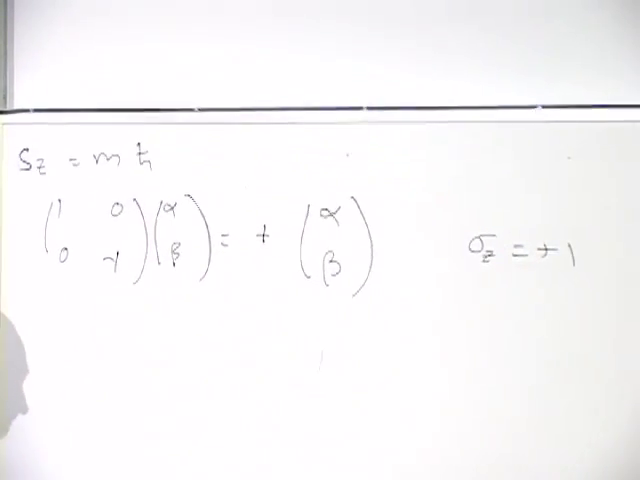
\includegraphics[width=0.74\textwidth]{lecture_08_figure_02.png}
\caption{二分量旋量在\(\sigma_z\)作用下滿足的\(+1\)本徵值方程。}
\lectureframe{00:34:57}
\end{figure}

對於本徵值\(+1\)，逐行相乘可得
\begin{equation}
\begin{pmatrix}
1\cdot\alpha+0\cdot\beta\\
0\cdot\alpha-\beta
\end{pmatrix}
=
\begin{pmatrix}
\alpha\\
-\beta
\end{pmatrix}
=
\begin{pmatrix}
\alpha\\
\beta
\end{pmatrix}.
\end{equation}
上方的方程自動成立；下方的方程則給出\(-\beta=\beta\)，所以\(\beta=0\)。歸一化條件要求\(|\alpha|=1\)；選擇任意的整體相位，使\(\alpha=1\)，便得到
\begin{equation}
|+z\rangle=
\begin{pmatrix}
1\\
0
\end{pmatrix}.
\end{equation}

對於本徵值\(-1\)，
\begin{equation}
\begin{pmatrix}
\alpha\\
-\beta
\end{pmatrix}
=
\begin{pmatrix}
-\alpha\\
-\beta
\end{pmatrix}.
\end{equation}
這時下方的方程自動成立，上方的方程給出\(\alpha=-\alpha\)，因此\(\alpha=0\)。令\(\beta=1\)，便得到
\begin{equation}
|-z\rangle=
\begin{pmatrix}
0\\
1
\end{pmatrix}.
\end{equation}

現在改為測量\(S_x\)。由於
\begin{equation}
\sigma_x
\begin{pmatrix}
\alpha\\
\beta
\end{pmatrix}
=
\begin{pmatrix}
0\cdot\alpha+\beta\\
\alpha+0\cdot\beta
\end{pmatrix}
=
\begin{pmatrix}
\beta\\
\alpha
\end{pmatrix},
\end{equation}
本徵值為\(+1\)的方程變成
\begin{equation}
\begin{pmatrix}
\beta\\
\alpha
\end{pmatrix}
=
\begin{pmatrix}
\alpha\\
\beta
\end{pmatrix}.
\end{equation}
兩個分量方程\(\beta=\alpha\)和\(\alpha=\beta\)表達的是同一個條件。歸一化後得到
\begin{equation}
2|\alpha|^2=1,
\end{equation}
因此，一個方便的選擇是
\begin{equation}
|+x\rangle
=
\frac{1}{\sqrt2}
\begin{pmatrix}
1\\
1
\end{pmatrix}.
\end{equation}

\begin{figure}[t]
\centering
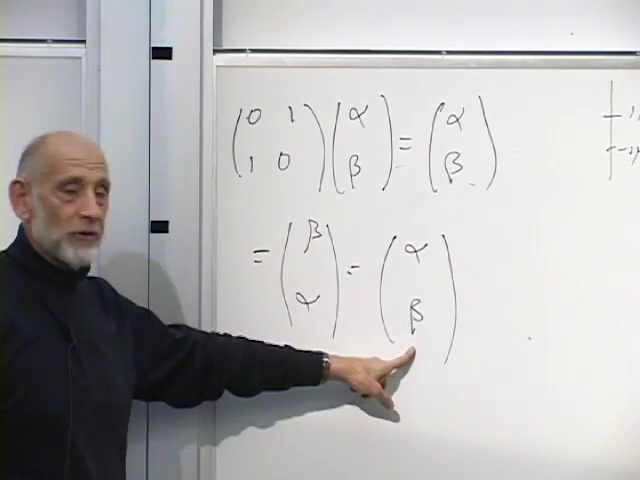
\includegraphics[width=0.74\textwidth]{lecture_08_figure_03.png}
\caption{本徵值為\(+1\)時，\(\sigma_x\)會交換兩個分量，因此必須滿足\(\alpha=\beta\)。}
\lectureframe{00:39:42}
\end{figure}

\begin{classroomqa}
\lecturetimestamp{00:40:13}
\audiencequestion{如果納入二分之一因子，本徵值會是二分之一嗎？}
\lecturerresponse{是的。泡利矩陣\(\sigma_x\)的本徵值是\(\pm1\)；而\(S_x=\sigma_x/2\)的本徵值是\(\pm\tfrac12\)。}
\end{classroomqa}

對於本徵值\(-1\)，
\begin{equation}
\begin{pmatrix}
\beta\\
\alpha
\end{pmatrix}
=
-
\begin{pmatrix}
\alpha\\
\beta
\end{pmatrix},
\end{equation}
所以
\begin{equation}
\beta=-\alpha,
\qquad
\alpha=-\beta.
\end{equation}
這兩個方程同樣表達相同條件。歸一化後，
\begin{equation}
|-x\rangle
=
\frac{1}{\sqrt2}
\begin{pmatrix}
1\\
-1
\end{pmatrix}.
\end{equation}
因此，\(z\)向上與\(z\)向下的等量疊加態，具有沿正\(x\)軸的極化；若兩者之間帶有相對負號，則具有沿負\(x\)軸的極化。

對於\(y\)方向，
\begin{equation}
\sigma_y
\begin{pmatrix}
\alpha\\
\beta
\end{pmatrix}
=
\begin{pmatrix}
-i\beta\\
i\alpha
\end{pmatrix}.
\end{equation}
兩個歸一化本徵向量為
\begin{equation}
|+y\rangle
=
\frac{1}{\sqrt2}
\begin{pmatrix}
1\\
i
\end{pmatrix},
\qquad
|-y\rangle
=
\frac{1}{\sqrt2}
\begin{pmatrix}
1\\
-i
\end{pmatrix},
\end{equation}
差別僅在整體相位。兩個態測得\(z\)向上的機率都是\(1/2\)，測得\(z\)向下的機率都是\(1/2\)。相對相位\(i\)不會顯現在這兩個機率中，卻能區分\(y\)極化和\(x\)極化。線性組合也可以描述沿任意方向極化的自旋，相關計算留待後續討論。

\begin{classroomqa}
\lecturetimestamp{00:44:22}
\audiencequestion{\(\sigma_y\)的\(i\)分量是否被配上了錯誤的本徵值？}
\lecturerresponse{這個符號的確可能配錯了本徵值。這裡無法確定正確的配法，因此不憑記憶下定論。}
\end{classroomqa}

直接計算可得
\begin{align}
\sigma_y\frac{1}{\sqrt2}
\begin{pmatrix}
1\\
i
\end{pmatrix}
&=
\frac{1}{\sqrt2}
\begin{pmatrix}
-i\,i\\
i
\end{pmatrix}
=
\frac{1}{\sqrt2}
\begin{pmatrix}
1\\
i
\end{pmatrix},\\
\sigma_y\frac{1}{\sqrt2}
\begin{pmatrix}
1\\
-i
\end{pmatrix}
&=
\frac{1}{\sqrt2}
\begin{pmatrix}
(-i)(-i)\\
i
\end{pmatrix}
=
-\frac{1}{\sqrt2}
\begin{pmatrix}
1\\
-i
\end{pmatrix}.
\end{align}
因此，\(+i\)對應本徵值\(+1\)；\(-i\)則對應本徵值\(-1\)。\footnote{口述時對應關係幾經反覆，仍未確定；此處的符號則以所示矩陣乘法的結果為準。}每個自旋二分之一態，包括沿任意方向極化的態，都是\(|+z\rangle\)和\(|-z\rangle\)的線性組合。

\section{自旋一與位置依賴的旋量}

對於自旋\(1\)，\(S_z\)的可能值為\(+1,0,-1\)，因此態空間是三維的。自旋\(1\)是整數自旋，對應玻色統計。我們要找出三個滿足相同角動量對易關係的\(3\times3\)矩陣。

以下給出一種對三個座標方向一視同仁的表示法。\footnote{\(S_y\)的符號依據\(00{:}48{:}50\)附近顯示的矩陣，也由\([S_x,S_y]=iS_z\)確定。若將這個符號反轉，所需的對易關係也會跟著反轉。}
\begin{equation}
\begin{aligned}
S_x
&=
i
\begin{pmatrix}
0&0&0\\
0&0&1\\
0&-1&0
\end{pmatrix},
&
S_y
&=
i
\begin{pmatrix}
0&0&1\\
0&0&0\\
-1&0&0
\end{pmatrix},\\
S_z
&=
i
\begin{pmatrix}
0&1&0\\
-1&0&0\\
0&0&0
\end{pmatrix}.
\end{aligned}
\end{equation}
每個矩陣都是\(i\)乘上一個實反對稱矩陣。每個矩陣各含有一個\(1\)、一個\(-1\)，並且與自身座標相對應的行和列皆為零：第一個對應\(S_x\)，第二個對應\(S_y\)，第三個對應\(S_z\)。這可以當作一個好記的口訣。在這種表示法中，\(S_z\)不是對角矩陣。

令
\begin{equation}
v=
\begin{pmatrix}
\alpha\\
\beta\\
\gamma
\end{pmatrix}.
\end{equation}
則
\begin{equation}
S_zv
=
\begin{pmatrix}
i\beta\\
-i\alpha\\
0
\end{pmatrix}.
\end{equation}
對於本徵值\(+1\)，
\begin{equation}
i\beta=\alpha,
\qquad
-i\alpha=\beta,
\qquad
0=\gamma.
\end{equation}
因此\(\beta=-i\alpha\)，且\(\gamma=0\)。歸一化條件給出\(2|\alpha|^2=1\)，所以
\begin{equation}
|m=+1\rangle
=
\frac{1}{\sqrt2}
\begin{pmatrix}
1\\
-i\\
0
\end{pmatrix}.
\end{equation}
對於本徵值\(-1\)，
\begin{equation}
i\beta=-\alpha,
\qquad
-i\alpha=-\beta,
\qquad
0=-\gamma,
\end{equation}
因此\(\beta=i\alpha\)、\(\gamma=0\)，並得到
\begin{equation}
|m=-1\rangle
=
\frac{1}{\sqrt2}
\begin{pmatrix}
1\\
i\\
0
\end{pmatrix}.
\end{equation}
最後，零本徵值方程給出\(\alpha=\beta=0\)，而\(\gamma\)仍可任意取值。歸一化後的解為
\begin{equation}
|m=0\rangle
=
\begin{pmatrix}
0\\
0\\
1
\end{pmatrix}.
\end{equation}
這三個本徵向量已經涵蓋整個三維空間，不存在其他本徵值。因子\(1/\sqrt2\)並非無關緊要；之後將這套代數應用於同位旋時，相同係數會出現在定量的實驗預測中。

\begin{classroomqa}
\lecturetimestamp{00:54:10}
\audiencequestion{這些自旋一本徵向量中的複數分量應該如何解讀？}
\lecturerresponse{當\(m=+1\)時，分量為\(1/\sqrt2,-i/\sqrt2,0\)；當\(m=-1\)時，分量為\(1/\sqrt2,i/\sqrt2,0\)；而當\(m=0\)時，分量為\(0,0,1\)。}
\end{classroomqa}

其他矩陣三元組也滿足相同的代數，且在物理上等價。上述對稱表示法的優點是平等看待三個方向，而且後面還會再用到它。

\subsection{恢復位置自由度}

現在把粒子的運動納入考量。自旋與位置、動量都對易，因此可以同時指定位置或動量以及一個自旋分量。位置與動量彼此不對易，不同的自旋分量之間也不對易。

運動中的自旋二分之一粒子以位置依賴的旋量描述：
\begin{equation}
\psi(x)=
\begin{pmatrix}
\psi_\uparrow(x)\\
\psi_\downarrow(x)
\end{pmatrix}.
\end{equation}
以下各量
\begin{equation}
\rho_{\uparrow_z}(x)=|\psi_\uparrow(x)|^2,
\qquad
\rho_{\downarrow_z}(x)=|\psi_\downarrow(x)|^2
\end{equation}
是位置與自旋的聯合機率密度。將它們相加，
\begin{equation}
\rho(x)=\psi^\dagger(x)\psi(x)
=|\psi_\uparrow(x)|^2+|\psi_\downarrow(x)|^2,
\end{equation}
便得到位置密度。若已知粒子在\(x\)處被偵測到，條件機率為
\begin{equation}
P(\uparrow_z\mid x)
=
\frac{|\psi_\uparrow(x)|^2}{\psi^\dagger(x)\psi(x)},
\qquad
P(\downarrow_z\mid x)
=
\frac{|\psi_\downarrow(x)|^2}{\psi^\dagger(x)\psi(x)},
\end{equation}
只要\(\rho(x)\neq0\)。因此，電子由一個二分量的空間波函數描述，局部的自旋振幅可以隨位置而變化。

運動中的自旋一粒子可寫成
\begin{equation}
\phi(x)=
\begin{pmatrix}
\phi_1(x)\\
\phi_2(x)\\
\phi_3(x)
\end{pmatrix}.
\end{equation}
在空間中的每一點，三個分量都構成上述同一自旋空間中的一個向量。自旋一粒子具有整數自旋，因此是玻色子。

\begin{classroomqa}
\lecturetimestamp{01:00:10}
\audiencequestion{\(\phi_1(x)\)本身就是自旋一的\(m=+1\)結果機率嗎？}
\lecturerresponse{不是。它是在所選三分量基底中的振幅。若要得到確定的自旋測量結果，先取相應歸一化本徵向量的左矢，將場投影到該左矢上，再取模平方。}
\end{classroomqa}

\begin{figure}[t]
\centering
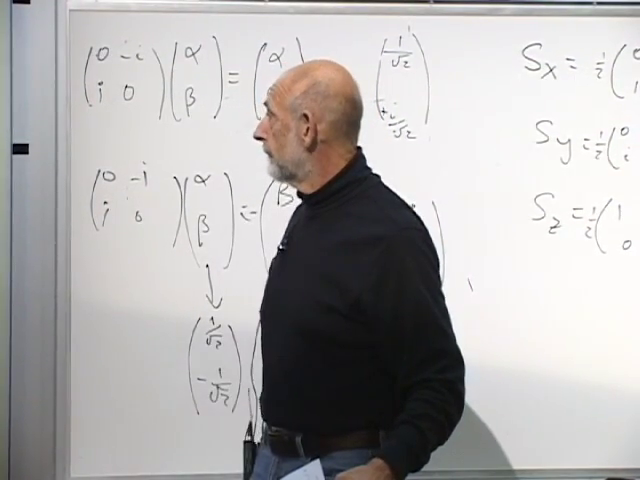
\includegraphics[width=0.82\textwidth]{lecture_08_figure_04.png}
\caption{歸一化的\(\sigma_y\)本徵向量，與三個自旋二分之一矩陣並列。}
\lectureframe{01:00:12}
\end{figure}

例如，
\begin{equation}
\begin{aligned}
|m=+1\rangle
&=
\frac{1}{\sqrt2}
\begin{pmatrix}
1\\
-i\\
0
\end{pmatrix}
\\
\Longrightarrow\quad\langle m=+1|
&=
\frac{1}{\sqrt2}
\begin{pmatrix}
1&i&0
\end{pmatrix}.
\end{aligned}
\end{equation}
因此，投影振幅為
\begin{align}
\langle m=+1|\phi(x)\rangle
&=
\frac{1}{\sqrt2}
\begin{pmatrix}
1&i&0
\end{pmatrix}
\begin{pmatrix}
\phi_1(x)\\
\phi_2(x)\\
\phi_3(x)
\end{pmatrix}\\
&=
\frac{\phi_1(x)+i\phi_2(x)}{\sqrt2}.
\end{align}
對三個本徵向量都套用相同規則，就能得到各自旋分量的密度。\footnote{明確修正\(\phi_1\)和\(\phi_2\)不一定是實數後，這些公式便完整描述了投影代數。若把它們當作實數，就會錯誤地消去區分\(m=+1\)與\(m=-1\)密度的干涉效應。}
\begin{align}
\rho_{+1}(x)
&=
\frac12\left|\phi_1(x)+i\phi_2(x)\right|^2,\\
\rho_{-1}(x)
&=
\frac12\left|\phi_1(x)-i\phi_2(x)\right|^2,\\
\rho_0(x)
&=
|\phi_3(x)|^2.
\end{align}
它們滿足
\begin{equation}
\begin{aligned}
\rho_{+1}(x)+\rho_{-1}(x)+\rho_0(x)
&=
|\phi_1(x)|^2+|\phi_2(x)|^2
\\
&\quad{}+|\phi_3(x)|^2
\\
&=
\phi^\dagger(x)\phi(x).
\end{aligned}
\end{equation}
若已知粒子在\(x\)處被偵測到，則
\begin{equation}
P(m\mid x)
=
\frac{\rho_m(x)}{\phi^\dagger(x)\phi(x)},
\end{equation}
只要\(\phi^\dagger(x)\phi(x)\neq0\)。一般的測量規則始終相同：取出目標歸一化本徵向量的左矢，將實際態投影到它上面，再取模平方。所得密度仍保留對位置的依賴。

更高自旋的矩陣較為複雜，但原理不變。

\begin{classroomqa}
\lecturetimestamp{01:07:31}
\audiencequestion{自旋三分之二的態空間有多大？}
\lecturerresponse{共有四個態，其中\(m=\tfrac32,\tfrac12,-\tfrac12,-\tfrac32\)。自旋二則有五個態。}
\end{classroomqa}

\begin{classroomqa}
\lecturetimestamp{01:07:55}
\audiencequestion{為什麼討論中出現了\(x,y,z\)，卻沒有時間方向？這套處理是非相對論性的嗎？}
\lecturerresponse{到目前為止，這套處理是非相對論性的。自旋和質量一樣，在粒子的靜止系中最容易描述；在其他慣性系中的描述，則由相應的洛倫茲變換得到。這個相對論性的步驟留待後續討論。}
\end{classroomqa}

狄拉克方程提供了相對論性的框架，也說明為什麼它的四分量波函數包含一個自旋雙重態。

\section{狄拉克矩陣與四分量旋量}

四分量狄拉克波函數滿足
\begin{equation}
i\frac{\partial\Psi}{\partial t}
=
-i\alpha_i\frac{\partial\Psi}{\partial x_i}
+m\beta\Psi,
\qquad i=1,2,3,
\end{equation}
其中重複的空間指標代表求和。因此，導數項就是
\begin{equation}
\alpha_1\frac{\partial\Psi}{\partial x}
+\alpha_2\frac{\partial\Psi}{\partial y}
+\alpha_3\frac{\partial\Psi}{\partial z}.
\end{equation}
對平面波而言，方程可化為代數形式
\begin{equation}
\omega\Psi=(\alpha_i k_i+m\beta)\Psi.
\end{equation}

\begin{classroomqa}
\lecturetimestamp{01:11:32}
\audiencequestion{兩處的\(m\)指的是同一件事嗎？}
\lecturerresponse{不是。一處將它用作空間指標，另一處則表示粒子的質量。將空間指標改記為\(i\)；當\(i\)出現兩次時，就要從\(1\)加到\(3\)求和。}
\end{classroomqa}

將頻率算符平方後，必須得到相對論關係式
\begin{equation}
\omega^2=\mathbf{k}^2+m^2.
\end{equation}
因此，對每個\(i\)，平方項都必須滿足
\begin{equation}
\alpha_i^2=I_4,
\qquad
\beta^2=I_4.
\end{equation}

\begin{classroomqa}
\lecturetimestamp{01:13:01}
\audiencequestion{\(\beta\)在\(\Psi\)的四個分量中各不相同嗎？}
\lecturerresponse{不是。只有一個矩陣\(\beta\)作用於整個四分量旋量，而且它滿足\(\beta^2=I_4\)。}
\end{classroomqa}

混合項必須消失。不同空間方向的矩陣彼此之間，以及每個\(\alpha_i\)與\(\beta\)之間，都必須滿足
\begin{equation}
\alpha_i\alpha_j+\alpha_j\alpha_i=0
\quad (i\neq j),
\qquad
\alpha_i\beta+\beta\alpha_i=0.
\end{equation}
等價地，
\begin{equation}
\{\alpha_i,\alpha_j\}=2\delta_{ij}I_4,
\quad
\{\alpha_i,\beta\}=0,
\quad
\{\beta,\beta\}=2I_4.
\end{equation}
每個矩陣都與其他不同的矩陣反對易；矩陣與自身的反對易子則等於單位矩陣的兩倍。

若沒有\(\beta\)，三個泡利矩陣已經提供了三個平方等於單位矩陣、且兩兩反對易的\(2\times2\)矩陣。質量項還要求第四個具有相同性質的矩陣。不存在符合這些條件的第四個\(2\times2\)矩陣，而\(3\times3\)矩陣也無法滿足這套代數。因此，最小表示的維度是\(4\times4\)。

一個\(4\times4\)矩陣可以分成四個\(2\times2\)區塊。在一種方便的表示法中，
\begin{equation}
\alpha_i=
\begin{pmatrix}
\sigma_i&0\\
0&-\sigma_i
\end{pmatrix},
\qquad i=1,2,3.
\end{equation}

\begin{figure}[t]
\centering
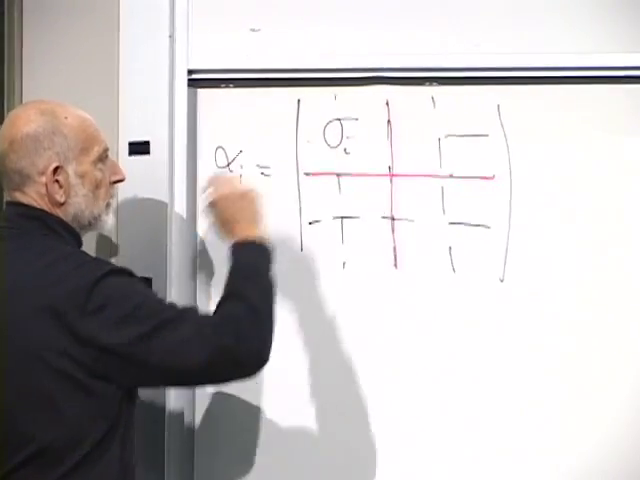
\includegraphics[width=0.68\textwidth]{lecture_08_figure_05.png}
\caption{狄拉克矩陣\(\alpha_i\)以\(2\times2\)區塊表示，\(\sigma_i\)和\(-\sigma_i\)位於對角線上。}
\lectureframe{01:17:23}
\end{figure}

\begin{classroomqa}
\lecturetimestamp{01:17:41}
\audiencequestion{早先的表示法中，\(\sigma_i\)區塊是不是以相反的方式排列？}
\lecturerresponse{是的。另一種表示法把它們放在非對角線位置。這兩種排列彼此等價，並由相似變換連結。}
\end{classroomqa}

在目前的表示法中，另一個矩陣是
\begin{equation}
\beta=
\begin{pmatrix}
0&I_2\\
I_2&0
\end{pmatrix},
\qquad
I_2=
\begin{pmatrix}
1&0\\
0&1
\end{pmatrix}.
\end{equation}
透過區塊矩陣乘法，只需進行一般\(2\times2\)矩陣的乘法，就能檢驗\(4\times4\)代數。

\begin{classroomqa}
\lecturetimestamp{01:19:17}
\audiencequestion{早先的表示法中，\(\beta\)是不是具有不同的符號或對角形式？}
\lecturerresponse{早先採用的是不同但在物理上等價的基底。基底變換會混合\(\Psi\)的四個分量，改變矩陣的形式，但不改變物理。}
\end{classroomqa}

\(\Psi\)的四個分量不是時空的四個座標，而是這套反對易代數能作用的最小向量空間中的座標。這裡有兩種不同的二重結構：分成\(2\times2\)區塊的結構，以及每個區塊內部的二分量泡利結構。先看下文將建立的詮釋，四種可能性可以整理如下：
\begin{equation}
\begin{array}{c|cc}
& S_z=+\tfrac12 & S_z=-\tfrac12\\ \hline
\omega>0 & (\omega>0,+\tfrac12) & (\omega>0,-\tfrac12)\\
\omega<0 & (\omega<0,+\tfrac12) & (\omega<0,-\tfrac12)
\end{array}.
\end{equation}
下一列代表負頻率的電子態，不是正電子。正電子將被詮釋為這組態全部填滿後所留下的一個電洞。

\section{靜止系能量的倍增與正電子}

在零動量處，最容易看出能量的二重結構。當\(\mathbf{k}=0\)時，平面波態在空間中為常數，空間導數項也就消失。靜止系方程\footnote{在\(01{:}23{:}38\)的畫面中，質量項暫時多出了一個因子\(i\)；\(01{:}24{:}05\)處的口頭更正則將它去除。}為
\begin{equation}
i\frac{\partial\Psi}{\partial t}=m\beta\Psi.
\end{equation}

\begin{figure}[t]
\centering
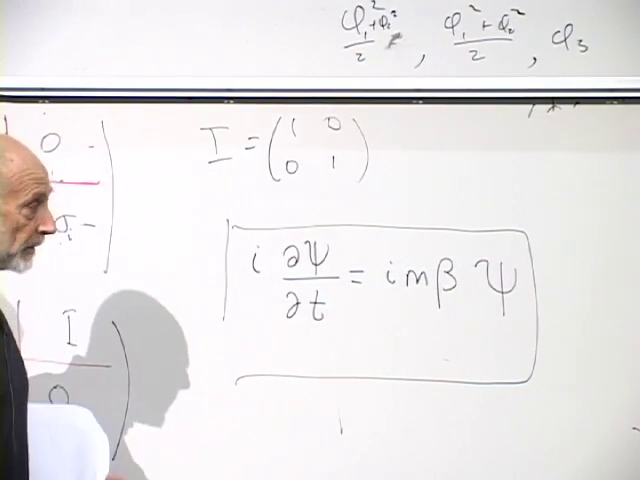
\includegraphics[width=0.76\textwidth]{lecture_08_figure_06.png}
\caption{零動量時空間導數消失，剩下修正後的靜止系方程\(i\partial_t\Psi=m\beta\Psi\)。}
\lectureframe{01:23:38}
\end{figure}

將四分量直欄向量分成上、下兩個二分量向量：
\begin{equation}
\Psi=
\begin{pmatrix}
\psi_+\\
\psi_-
\end{pmatrix}.
\end{equation}

\begin{classroomqa}
\lecturetimestamp{01:24:47}
\audiencequestion{標記 \(\psi_+\) 和 \(\psi_-\) 已經代表正能量和負能量了嗎？}
\lecturerresponse{還沒有。在這個階段，它們只是上、下兩個二分量區塊的名稱，還沒有求出它們對應的能量組合。}
\end{classroomqa}

\begin{classroomqa}
\lecturetimestamp{01:25:10}
\audiencequestion{分成兩部分的四分量列向量代表什麼？}
\lecturerresponse{它仍是同一個四分量狄拉克旋量，只是按照矩陣的區塊形式重新排列。每一半都是二分量物件，兩個這樣的物件合起來就是原本的四分量列向量。}
\end{classroomqa}

矩陣 \(\beta\) 會交換這兩個區塊：
\begin{equation}
\beta
\begin{pmatrix}
\psi_+\\
\psi_-
\end{pmatrix}
=
\begin{pmatrix}
\psi_-\\
\psi_+
\end{pmatrix}.
\end{equation}
因此，靜止系中的方程變為
\begin{equation}
i\frac{\partial\psi_+}{\partial t}=m\psi_-,
\qquad
i\frac{\partial\psi_-}{\partial t}=m\psi_+.
\end{equation}

有兩種自然的做法。再取一次時間導數可以將系統解耦；不過，將兩個方程相加與相減，就能立即將它們對角化。具體而言，
\begin{align}
i\frac{\partial}{\partial t}(\psi_++\psi_-)
&=m(\psi_++\psi_-),\\
i\frac{\partial}{\partial t}(\psi_+-\psi_-)
&=-m(\psi_+-\psi_-).
\end{align}
定義
\begin{equation}
\chi_+=\psi_++\psi_-,
\qquad
\chi_-=\psi_+-\psi_-,
\end{equation}
便得到兩個互相獨立的方程：
\begin{equation}
i\partial_t\chi_+=m\chi_+,
\qquad
i\partial_t\chi_-=-m\chi_-.
\end{equation}
若時間依賴具有確定頻率 \(e^{-i\omega t}\)，和所對應的頻率為
\begin{equation}
\omega=+m,
\end{equation}
差所對應的頻率則為
\begin{equation}
\omega=-m.
\end{equation}
這正是先前一維例子中出現的正、負能量雙重結構：相對論方程再次具有正能量與負能量的電子解。因此，區塊的雙重結構分解為正能量與負能量兩個分支。純粹的靜止態可以寫成
\begin{equation}
\Psi_{\omega=+m}=
\begin{pmatrix}
\xi\\
\xi
\end{pmatrix},
\qquad
\Psi_{\omega=-m}=
\begin{pmatrix}
\xi\\
-\xi
\end{pmatrix},
\end{equation}
其中 \(\xi\) 仍是任意的二分量物件。

相加與相減已經分解了一種雙重結構，但 \(\xi\) 的兩個分量仍然存在。泡利矩陣作用於這一對剩餘分量。這一對與自旋相關；不過，還必須通過下文所述的旋轉或守恆定律檢驗，才能確認這一點。

\begin{classroomqa}
\lecturetimestamp{01:32:23}
\audiencequestion{可以把自旋看作外層的雙重結構，把能量正負看作內層的雙重結構嗎？}
\lecturerresponse{可以。這兩種因子的排列順序彼此等價，可以交換哪個指標寫在前面；這只會重新排列四個分量。}
\end{classroomqa}

負頻率分支引出了狄拉克海的詮釋。負頻率被賦予負的電子能量。將所有負能量電子態填滿，便能在泡利不相容原理允許的範圍內，盡可能降低能量，因為每個完整的費米子態只能容納一個電子。完全填滿的負能量海於是稱為真空。

將這個填滿的海中的一個電子提升到正能量態。結果會有一個正能量電子，以及一個未被佔據的負能量態。移去一個負能量會使能量升高，因此這個空穴具有正的激發能；由於少了一個電子，它也帶有與電子相反的電荷。這個空穴就是正電子。

\begin{classroomqa}
\lecturetimestamp{01:32:57}
\audiencequestion{可以再說明一次正電子的詮釋嗎？}
\lecturerresponse{兩個區塊相加得到正頻率，兩者相減則得到負頻率。負頻率解是負能量電子態；真空則是將這些態全部填滿後的狀態。把一個已填入的電子提升到正能量後，便同時留下正能量電子和一個空穴。這個具有正能量、帶相反電荷的空穴就是正電子。}
\end{classroomqa}

因此，這套代數同時帶來兩項結果：正能量與負能量分支，形成粒子--反粒子結構；以及與自旋二分之一相關的剩餘二分量結構。引人注目的是，這兩者都來自能夠滿足相對論性反對易關係的最小矩陣。當時，自旋才剛被發現是一種經驗性質；在這樣的歷史背景下，這套數學構造竟然導出具有自旋的粒子以及反粒子分支，結果十分驚人。

\begin{classroomqa}
\lecturetimestamp{01:35:14}
\audiencequestion{負能量電子本身就是正電子嗎？}
\lecturerresponse{不是。真空中的負能量電子態都已填滿。正電子是這些已填滿的態中少了一個電子，也就是一個空穴，而不是負能量電子。}
\end{classroomqa}

空穴也可以參與躍遷。正電子具有正能量，是因為它代表少了一個負能量電子。如果一個正能量電子填入空穴，電子與正電子便會湮滅，但能量必須由其他東西帶走，通常是光子。用狄拉克海的說法，就是一個電子填入原本未被佔據的負能量態。同樣的能量釋放，也可以想成原子中的激發態電子降至較低能階：電子向下躍遷時會放出光子。

\begin{classroomqa}
\lecturetimestamp{01:36:39}
\audiencequestion{為什麼能量較高的負能量電子不會落入空穴？}
\lecturerresponse{這個問題混淆了兩種情況。正能量電子填入空穴，屬於電子--正電子湮滅，能量由光子帶走。負能量海中的電子發生躍遷則是另一種過程，下面會再討論。}
\end{classroomqa}

零動量的計算本身已經表明，分離出能量正負後，仍有二重簡併。但兩個態的簡併本身，並不能證明它們具有角動量。

\begin{classroomqa}
\lecturetimestamp{01:37:44}
\audiencequestion{零動量計算如何證明剩下的兩個態代表自旋？}
\lecturerresponse{可以把這兩個態稱為自旋向上和自旋向下；完整方程中也會出現泡利矩陣，但這些都還不足以構成證明。必須證明這一對態在空間旋轉下如何變換，或者證明賦予它們自旋後，總角動量在交互作用和碰撞中守恆。這項論證留待後續討論。}
\end{classroomqa}

對於正能量的靜止態，上、下兩個區塊相等：
\begin{equation}
\Psi_{\omega=+m}=
\begin{pmatrix}
\xi\\
\xi
\end{pmatrix}.
\end{equation}
要確立 \(\xi\) 構成角動量二重態，仍需要前述的旋轉論證或守恆論證；光是數出兩個分量，並不能得出這個結論。

\begin{classroomqa}
\lecturetimestamp{01:40:46}
\audiencequestion{即使能量不同，另一個電子也能和這個正電子湮滅嗎？}
\lecturerresponse{可以。電子沒有各自獨立的身分，任何可用的電子都可以填入空穴。初始能量與動量的差異，會反映在放出光子的數量與能量上。}
\end{classroomqa}

空穴圖像也能解釋完全發生在負能量海內部的躍遷。假設一個已佔據的負能量態移入空穴，原來的空穴便被填滿，但該電子原先所在的態現在空了。於是空穴移動了。換句話說，正電子改變了能量並放出輻射。

\begin{classroomqa}
\lecturetimestamp{01:42:12}
\audiencequestion{為什麼相鄰的負能量能階不能接連落入空穴？}
\lecturerresponse{它們可以使空穴從一個能階移到另一個能階。電子落入原來的空穴後，會在它原先的能量處留下新空穴，因此原本的正電子就變成能量不同的正電子。能量差由光子帶走。}
\end{classroomqa}

\begin{classroomqa}
\lecturetimestamp{01:44:39}
\audiencequestion{為什麼這不會造成無止盡的向下輻射級聯？}
\lecturerresponse{因為能量和動量必須同時守恆，這兩項守恆定律不允許這種不受限制的過程。普通的自由電子也有同樣的限制：它不能只靠在空無一物的空間中放出光子，就不斷降低能量。}
\end{classroomqa}

\chapter{拉格朗日量、場與局域粒子過程}

玻色子場、費米子場和電磁場都遵循波動方程。這些方程涉及場本身，以及場對空間和時間的導數。雖然可以為每個場分別列出運動方程，但拉格朗日量能將整個系統濃縮為一個表示式。將尤拉--拉格朗日法則應用於這個表示式，就能一次得到所有場的方程。

這種構造與作用量取駐值密切相關。此處的直接目標更為具體：確認場的拉格朗日量依賴哪些量，用它推導幾個經典方程，再以量子力學的觀點重新詮釋相同的場表示式。在量子理論中，拉格朗日量支配粒子的運動與交互作用，最終也決定碰撞的振幅與截面。

\section{場方程的簡潔表述}

對於單一標量場，拉格朗日密度取決於場及其一階導數，
\begin{equation}
\mathcal L
=
\mathcal L\!\left(\phi,\partial_t\phi,\partial_x\phi,\ldots\right)
=
\mathcal L\!\left(\phi,\partial_\mu\phi\right).
\end{equation}
計算時，明確列出時間導數與空間導數往往更方便；記號\(\partial_\mu\phi\)則以相對論形式概括同一組導數。

\begin{figure}[htbp]
\centering
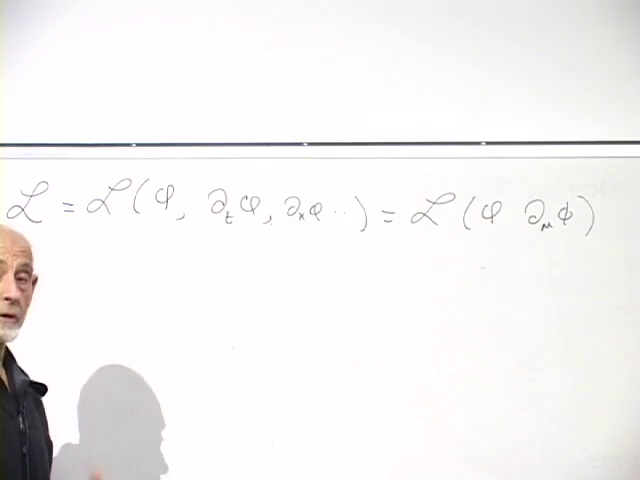
\includegraphics[width=0.82\textwidth]{lecture_09_figure_03.png}
\caption{標量場的拉格朗日量對場及其時空導數的依賴關係。}
\lectureframe{00:03:56}
\end{figure}

場的尤拉--拉格朗日方程為
\begin{equation}
\frac{\partial}{\partial t}
\frac{\partial\mathcal L}{\partial\dot\phi}
+
\frac{\partial}{\partial x}
\frac{\partial\mathcal L}{\partial\phi_x}
+
\frac{\partial}{\partial y}
\frac{\partial\mathcal L}{\partial\phi_y}
+
\frac{\partial}{\partial z}
\frac{\partial\mathcal L}{\partial\phi_z}
=
\frac{\partial\mathcal L}{\partial\phi},
\end{equation}
其中
\begin{equation}
\dot\phi=\frac{\partial\phi}{\partial t},
\qquad
\phi_x=\frac{\partial\phi}{\partial x},
\qquad
\phi_y=\frac{\partial\phi}{\partial y},
\qquad
\phi_z=\frac{\partial\phi}{\partial z}.
\end{equation}
若\(\mathcal L\)包含多個場，就對每個場各應用一次這條規則。所得結果便是整組運動方程。

最簡單的標量場例子是
\begin{equation}
\begin{split}
\mathcal L
&=
\frac12\dot\phi^2
-\frac12\phi_x^2
-\frac12\phi_y^2
-\frac12\phi_z^2
-V(\phi)
\\
&=
\frac12\dot\phi^2-\frac12(\boldsymbol\nabla\phi)^2-V(\phi).
\end{split}
\end{equation}
空間導數項的符號與時間導數項相反。逐項微分可得
\begin{align}
\frac{\partial\mathcal L}{\partial\dot\phi}&=\dot\phi,
&
\frac{\partial\mathcal L}{\partial\phi_i}&=-\phi_i,
&
\frac{\partial\mathcal L}{\partial\phi}&=-V'(\phi),
\end{align}
因此
\begin{equation}
\ddot\phi-\nabla^2\phi=-V'(\phi).
\end{equation}

\begin{figure}[htbp]
\centering
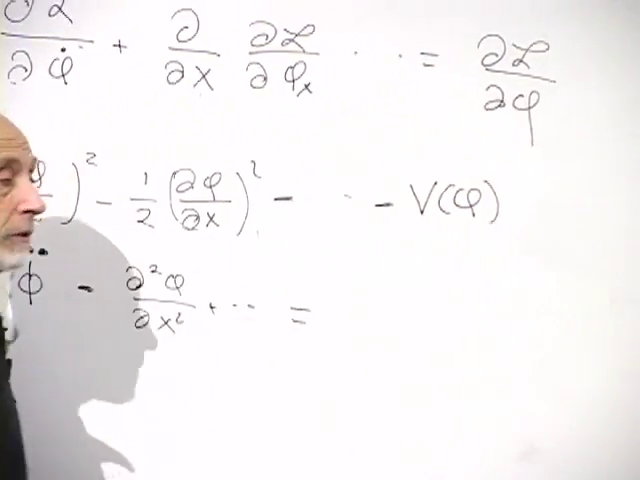
\includegraphics[width=0.74\textwidth]{lecture_09_figure_04.png}
\caption{尤拉--拉格朗日方程、標量場拉格朗日量，以及由\(V(\phi)\)所產生的場方程。}
\lectureframe{00:08:23}
\end{figure}

這就是標量場拉格朗日量所產生的方程。\editorialnote{保留的畫面左側遭到裁切；根據緊接著的口頭推導，可以確定此處顯示的補全內容。}

這裡\(V(\phi)\)是場的勢能密度。\(V\)中的常數項不影響這條方程，因為它的導數為零。線性勢在代數上雖然可行，卻沒有下界：場的能量可以一路降至負無窮。因此，第一個穩定的例子是
\begin{equation}
V(\phi)=\frac12m^2\phi^2,
\qquad
V'(\phi)=m^2\phi,
\end{equation}
它導出
\begin{equation}
\ddot\phi-\nabla^2\phi=-m^2\phi.
\end{equation}

為了看出\(m\)的物理意義，代入平面波
\begin{equation}
\phi(\mathbf x,t)=\phi_0e^{i\omega t-i\mathbf k\cdot\mathbf x}.
\end{equation}
於是
\begin{equation}
\ddot\phi=-\omega^2\phi,
\qquad
\nabla^2\phi=-\mathbf k^2\phi,
\end{equation}
波動方程便成為
\begin{equation}
-\omega^2\phi+\mathbf k^2\phi=-m^2\phi.
\end{equation}
消去\(\phi\)後，得到
\begin{equation}
\omega^2=\mathbf k^2+m^2.
\end{equation}
在\(\hbar=c=1\)單位制中，頻率對應能量，波數對應動量。因此
\begin{equation}
E^2=\mathbf p^2+m^2,
\end{equation}
或者，恢復\(c\)的冪次後，\(E^2=\mathbf p^2c^2+m^2c^4\)。參數\(m\)就是場的一個量子的質量。

可以直接在簡潔的表示式層次要求洛倫茲不變性。若\(\mathcal L\)是洛倫茲純量，它所導出的運動方程就是洛倫茲不變的。時間導數與空間導數之間的相對符號，正是狹義相對論中熟悉的時空符號差異。

\section{非線性與耦合的經典場}

場的高次項會帶來新的行為。若
\begin{equation}
V(\phi)=\frac12m^2\phi^2+g\phi^3,
\end{equation}
則
\begin{equation}
\ddot\phi-\nabla^2\phi=-m^2\phi-3g\phi^2.
\end{equation}
拉格朗日量中的二次項會導出場的線性方程；三次及更高次項則會導出非線性方程。

波包的運動清楚呈現了這項差異。對於線性方程，向右行進的波包與向左行進的波包可以相加，形成另一個解。兩者重疊並干涉一段時間，接著彼此穿越，離開時仍保持原有形狀。若有非線性項，波包便會彼此影響；它們可能散射、變形，或分裂成更複雜的波。線性波暫時干涉並不代表交互作用；波包持續改變，才是非線性的表徵。

兩個標量場也會呈現相同的模式。令
\begin{align}
\mathcal L
&=
\frac12(\partial_\mu\phi)(\partial^\mu\phi)
+\frac12(\partial_\mu\rho)(\partial^\mu\rho)
-V(\phi,\rho),
\\
V(\phi,\rho)
&=
\frac12m^2\phi^2+\frac12M^2\rho^2+\rho\phi^2.
\end{align}
若沒有最後一項，兩個方程彼此獨立：
\begin{equation}
\ddot\phi-\nabla^2\phi=-m^2\phi,
\qquad
\ddot\rho-\nabla^2\rho=-M^2\rho.
\end{equation}
它們描述兩種粒子的量子，質量分別為\(m\)與\(M\)。加入混合項後，
\begin{align}
\ddot\phi-\nabla^2\phi&=-m^2\phi-2\rho\phi,
\\
\ddot\rho-\nabla^2\rho&=-M^2\rho-\phi^2.
\end{align}
每個方程現在都包含另一個場。這些方程彼此耦合，而且是非線性的：一個\(\phi\)波包會散射一個\(\rho\)波包，反之亦然。導數項決定能量--動量關係；未微分的二次項決定質量；混合的高次項則描述交互作用。這就是基本的經典模式。

\section{狄拉克場與標量耦合}

狄拉克場的方程對時間是一階的。以下以一維簡寫，並假設可推廣至三個空間方向，其項的結構為
\begin{equation}
i\dot\Psi
\simeq
i\alpha\frac{\partial\Psi}{\partial x}+m\beta\Psi,
\qquad
i\boldsymbol\alpha\cdot\boldsymbol\nabla\Psi
=i\sum_i\alpha_i\frac{\partial\Psi}{\partial x_i}.
\end{equation}
矩陣\(\alpha_i\)與\(\beta\)作用於\(\Psi\)的各個分量。相應的拉格朗日量包含一個對\(\partial_t\Psi\)呈線性的項、一個涉及\(\alpha_i\)的空間導數雙線性項，以及質量雙線性項\(m\Psi^\dagger\beta\Psi\)。此處只需掌握這項結構事實。\editorialnote{原文嘗試寫出的狄拉克拉格朗日量中，正負號、括號及\(i\)的位置都明確未定，因此無法據此推定任何依賴慣例的精確公式。}

\begin{figure}[htbp]
\centering
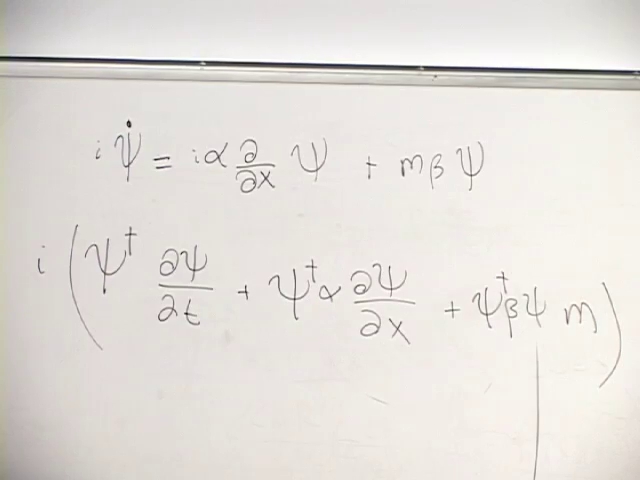
\includegraphics[width=0.76\textwidth]{lecture_09_figure_05.png}
\caption{狄拉克場討論中的時間導數項、空間導數項與質量項。}
\lectureframe{00:25:37}
\end{figure}

\begin{classroomqa}
\lecturetimestamp{00:26:37}
\audiencequestion{嘗試寫出的狄拉克拉格朗日量中，括號的位置是否正確？也就是說，\(i\)是否乘上整個表示式？}
\lecturerresponse{此處無法有把握地確定括號的位置，而且結構上的重點也不需要它：確實存在一個能導出狄拉克方程的拉格朗日量。}
\end{classroomqa}

現在加入標量場\(\phi\)。直接取乘積\(\Psi^\dagger\Psi\,\phi\)並不是洛倫茲純量。若插入質量項中出現的同一個狄拉克矩陣，就得到
\begin{equation}
\mathcal L_{\mathrm{int}}
\propto
\Psi^\dagger\beta\Psi\,\phi.
\end{equation}
換句話說，\(\Psi^\dagger\beta\Psi\)是標量狄拉克雙線性。對完整拉格朗日量作變分，會在狄拉克方程中加入一項，其正比於\(\phi\)；在標量方程中則加入一個正比於\(\Psi^\dagger\beta\Psi\)的源項。兩個場會彼此散射。

\begin{classroomqa}
\lecturetimestamp{00:28:03}
\audiencequestion{標量--費米子交互作用中插入的\(\beta\)，是否與狄拉克質量項中的\(\beta\)相同？}
\lecturerresponse{是，同一個狄拉克矩陣。}
\end{classroomqa}

比較
\begin{equation}
m\Psi^\dagger\beta\Psi
\qquad\hbox{and}\qquad
\Psi^\dagger\beta\Psi\,\phi
\end{equation}
可以看出，這種耦合的形式就像以標量場取代質量參數。接近本章末尾討論具有非零真空值的場時，還會再看到這個觀察。

到目前為止，這裡的詮釋都屬於經典描述：波包散射其他波包。場成為算符後，同一套代數便有了更明確的粒子意義。

\section{量子場的冪次所代表的過程}

實標量量子場同時包含產生算符與湮滅算符。示意地寫成
\begin{equation}
\phi(x)\sim A^+(x)+A^-(x),
\end{equation}
其中\(A^+\)產生一個量子，\(A^-\)湮滅一個量子。因此，\(\phi^3(x)\)包含四種局域過程：
\begin{equation}
\phi^3
\sim
(A^+)^3+(A^+)^2A^-+A^+(A^-)^2+(A^-)^3,
\end{equation}
以下的示意解讀省略了排序細節與數值係數。粒子數的四種變化分別是
\begin{equation}
3\longrightarrow0,
\qquad
0\longrightarrow3,
\qquad
2\longrightarrow1,
\qquad
1\longrightarrow2.
\end{equation}
三個場因子都作用在同一點\(x\)。因此，一個三次項就包含三個粒子湮滅、三個粒子產生、兩個量子合併成一個，以及一個量子分裂成兩個。在物理振幅中，能量--動量守恆之後可能排除其中一些局域解讀；但它們都存在於算符乘積本身。

二次自由項的作用則不同。先暫不考慮相鄰點\(x\)與\(x'\)之間差值的歸一化因子：
\begin{equation}
\partial_x\phi
\ \propto\
\phi(x)-\phi(x').
\end{equation}
將差值平方並展開，可得以下項的結構：
\begin{align}
\frac12(\partial_x\phi)^2
&\ \propto\
\frac12\bigl[\phi(x)-\phi(x')\bigr]^2
\\
&=
\frac12\phi(x)^2
+\frac12\phi(x')^2
-\phi(x)\phi(x').
\end{align}
每個同一點的平方項都有幾種算符解讀：可以在同一點產生兩個量子、湮滅兩個量子，或在該點湮滅一個量子後再將它產生。這些項不會使粒子從一處移動到另一處。交叉項則可以在\(x'\)湮滅一個量子，並在\(x\)產生該量子，反向過程也可以。因此它相當於最近鄰躍遷項。反覆作用的因子會將粒子從\(x\)帶至\(x'\)，再到\(x''\)，如此繼續。二次導數項支配自由傳播；三次及更高次項則使粒子散射、產生與湮滅。

\begin{classroomqa}
\lecturetimestamp{00:36:07}
\audiencequestion{導數的有限差分表示式是否應包含間隔\(x-x'\)？}
\lecturerresponse{是。將間隔記為\(L\)後，差值平方會帶出因子\(L^{-2}\)。這個數值因子會改變係數，但不影響躍遷的詮釋。}
\end{classroomqa}

恢復間隔後，得到
\begin{align}
\frac12(\partial_x\phi)^2
&\longrightarrow
\frac{1}{2L^2}\bigl[\phi(x)-\phi(x')\bigr]^2
\\
&=
\frac{1}{2L^2}\phi(x)^2
+\frac{1}{2L^2}\phi(x')^2
-\frac{1}{L^2}\phi(x)\phi(x').
\end{align}

質量項也是二次項，但不含導數：
\begin{equation}
\frac12m^2\phi(x)^2.
\end{equation}
就單粒子而言，可以將它解讀為入射量子在同一點被吸收後再重新發射。它不會使量子移動；它為量子在該處的存在賦予權重，或者說，在這個意義上計數。同一個算符平方也包含雙產生與雙湮滅的解讀。因此，就運動而言，關鍵差異在於連結相鄰點的交叉項，以及作用於單一點內的質量插入。

\section{量子電動力學的局域頂點}

這些基本粒子過程的示意圖，正是費曼圖的起點。核心例子是量子電動力學，也就是描述電子、正電子與光子的理論。

狄拉克方程具有正能量模與負能量模。依較早期的說法，\(\Psi\)包含兩類模式的湮滅算符，而\(\Psi^\dagger\)則包含相應的產生算符。移除一個負能量電子，可以重新詮釋為產生一個正能量正電子。重新標記後，方便的示意分解為
\begin{align}
\Psi
&\sim
C^-_{e^-}+C^+_{e^+},
\\
\Psi^\dagger
&\sim
C^+_{e^-}+C^-_{e^+}.
\end{align}
因此，\(\Psi\)會湮滅電子或產生正電子；\(\Psi^\dagger\)則會產生電子或湮滅正電子。這個簡寫不包含任何歸一化因子、自旋標記或動量積分。

QED交互作用將狄拉克流與電磁向量勢耦合。在此使用的分量記號中，其結構為
\begin{equation}
\mathcal L_{\mathrm{QED,int}}
\sim
e\left(
\Psi^\dagger\Psi\,A_0
+
\Psi^\dagger\boldsymbol{\alpha}\Psi\mathbin{\boldsymbol{\cdot}}\mathbf A
\right),
\end{equation}
其中
\begin{equation}
J^0=\Psi^\dagger\Psi,
\qquad
\mathbf J=\Psi^\dagger\boldsymbol{\alpha}\Psi.
\end{equation}
符號\(\sim\)很重要：時間項與空間項的相對符號取決於度規和向量勢的慣例。不依賴慣例的說法是，四維流與四維勢作縮並。\editorialnote{原文給出了流的時間與空間分量，但未確定分量縮並所採用的度規慣例。}

光子場 \(A_\mu\) 本身包含光子的產生算符和湮滅算符。它的向量性質還承載光子的極化---這個小小的方向性 ``標誌''，以及光子的動量。

\begin{classroomqa}
\lecturetimestamp{00:44:28}
\audiencequestion{當\(A_\mu\)是向量，而費米子因子乍看之下是純量時，交互作用怎麼會是純量？}
\lecturerresponse{費米子也提供四維向量：\(\Psi^\dagger\Psi\)是時間分量，\(\Psi^\dagger\boldsymbol\alpha\Psi\)是空間分量。將這個流與\(A_\mu\)縮並，就會得到純量。}
\end{classroomqa}

將\(\Psi^\dagger\)、\(\Psi\)和\(A_\mu\)的算符內容相乘，就會得到同一個局域頂點的四種常見解讀：
\begin{enumerate}
\item 電子發射光子；
\item 電子吸收光子；
\item 電子與正電子湮滅，產生光子；
\item 光子產生電子--正電子對。
\end{enumerate}
以第一種解讀為例，\(\Psi\)湮滅入射電子，\(\Psi^\dagger\)產生出射電子，而光子場則產生光子。若選用光子的湮滅部分，便得到吸收過程；若選用正電子部分，則得到正負電子對的湮滅或產生。一個局域項就包含了這一整組過程。

在費米子流圖中，正電子線上的箭頭方向與正電子的傳播方向相反。依照這項慣例，費米子流的箭頭會連續穿過每一個允許的QED頂點。四種解讀的差異在於外線移至入射側或出射側，而不是費米子流線中斷。

每一種解讀都帶有相同的係數\(e\)，也就是此處微觀慣例下的電荷。這個係數是電荷\(e\)，不是精細結構常數，儘管兩者密切相關。頂點振幅正比於\(e\)；納入所有運動學與歸一化因子後，相應的機率尺度正比於\(e^2\)。

\begin{classroomqa}
\lecturetimestamp{00:49:44}
\audiencequestion{將光子解讀為轉變成電子--正電子時，頂點係數是否與其他解讀相同？}
\lecturerresponse{是，電荷係數同樣是\(e\)。}
\end{classroomqa}

\begin{classroomqa}
\lecturetimestamp{00:49:59}
\audiencequestion{機率沒有單位，是否仍需要一個尺度因子？}
\lecturerresponse{在此採用的自然微觀慣例中，電荷\(e\)是無因次的。它決定振幅的尺度，而它的平方決定機率的尺度。}
\end{classroomqa}

可以想像電子撞上牆壁並突然停下。能量與動量有一定機率以光子的形式離開。輻射振幅中基本的電磁因子是\(e\)，因此機率尺度包含\(e^2\)。這裡指出的是耦合因子；實際機率也取決於電子的狀態與運動學。

\begin{figure}[htbp]
\centering
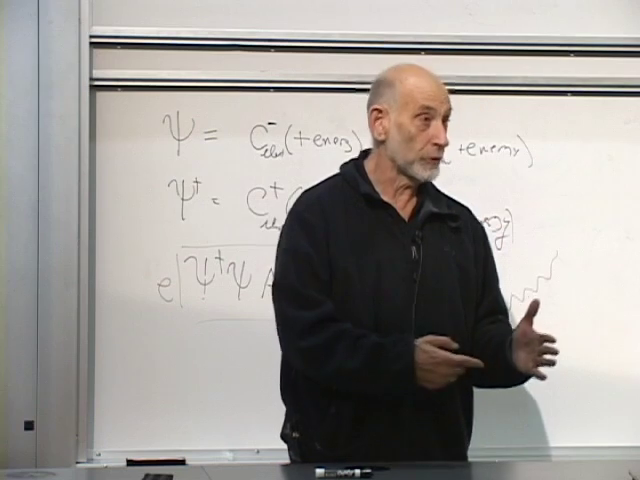
\includegraphics[width=0.78\textwidth]{lecture_09_figure_06.png}
\caption{\(\Psi\)與\(\Psi^\dagger\)所含的電子與正電子算符，以及電子--光子交互作用示意圖。}
\lectureframe{00:50:39}
\end{figure}

\begin{classroomqa}
\lecturetimestamp{00:51:15}
\audiencequestion{電荷有單位嗎？}
\lecturerresponse{在此使用的自然微觀慣例中，電荷沒有單位。宏觀電荷常以庫侖表示，但粒子理論以選定的基本單位為基準來衡量電荷。在普朗克單位或其他自然單位制中，這些量都以純數表示。}
\end{classroomqa}

這是慣例與尺度的差異。庫侖適合表示導線中的電流；無因次耦合則適合描述微觀振幅。\editorialnote{在00有個簡短提問：52：37--00：53：15關於如何``分組''含電荷的項，原文表述嚴重受損，因此無法確定其意圖。}

基本QED交互作用中的三個場，都在同一個時空點取值。頂點本身沒有內部時間延遲。

\begin{classroomqa}
\lecturetimestamp{00:53:19}
\audiencequestion{電子的吸收與再發射，以及光子的發射，是同時發生的嗎？還是方程中內含某種延遲？}
\lecturerresponse{在基本頂點處，所有算符都在同一個時空點取值。因此，這個基本過程中各項作用之間沒有延遲。}
\end{classroomqa}

\begin{classroomqa}
\lecturetimestamp{00:53:57}
\audiencequestion{每一種守恆量都必須各自守恆嗎？}
\lecturerresponse{是。電荷就是必須各自守恆的量之一。}
\end{classroomqa}

電荷守恆在圖像和代數中都看得出來。若入射電子變成出射正電子，電荷就會反轉，因此這不是允許的QED頂點。若時間軸朝上，電子箭頭朝上，正電子箭頭則朝下；合法的頂點總會有一條貫穿頂點的費米子箭頭。在代數上，交互作用包含一個\(\Psi\)和一個\(\Psi^\dagger\)。前者在湮滅電子或產生正電子時，會使電荷增加一個單位；後者則使電荷減少一個單位。兩者的效果相互抵消。

\begin{classroomqa}
\lecturetimestamp{00:56:05}
\audiencequestion{方框中的電子--光子表示式就是完整的QED拉格朗日量嗎？}
\lecturerresponse{不是。它是交互作用項。支配傳播的自由光子二次項與狄拉克二次項都尚未寫出。}
\end{classroomqa}

\begin{classroomqa}
\lecturetimestamp{00:56:35}
\audiencequestion{經典拉格朗日量是推導出來的，而量子拉格朗日量則是猜測後再加以檢驗的嗎？動能減去勢能的結構在量子力學中也保留嗎？}
\lecturerresponse{動能減去勢能的形式仍然保留：時間導數提供動能形式，空間梯度將這種形式推廣，而未微分的場項提供勢能形式。量子拉格朗日量是更基本的描述。在含有大量量子的狀態中，同一個拉格朗日量會導出經典波動方程。候選拉格朗日量依據物理原理與更深層的理論提出，再透過碰撞實驗加以確立或排除。}
\end{classroomqa}

大量子佔據的極限，說明了為何同一個表示式能支配量子粒子理論及其經典波。這種一致性並非事後另行強加的結果；經典場是大量量子的集體行為。反過來說，實驗碰撞能直接呈現基本頂點，讓人得以極精確地確定QED與標準模型中的交互作用。

\section{交叉與時空守恆定律}

局域頂點的外線可以在入射位置與出射位置之間互換。將一條出射粒子線移到入射側時，必須將它重新詮釋為相應的反粒子，反過來也一樣。從這個角度看，同一個電子--正電子--光子算符，可以有發射、吸收、正負電子對湮滅、正負電子對產生，甚至所有粒子皆從入射側進入的局域解讀。

\begin{classroomqa}
\lecturetimestamp{00:59:34}
\audiencequestion{將基本頂點圖旋轉後，它仍代表一種有效的局域解讀嗎？}
\lecturerresponse{是。外線可以在入射與出射位置之間移動，並相應地將粒子--重新詮釋為反粒子，或反之。}
\end{classroomqa}

局域算符的解讀還不是完整的物理過程。必須對頂點可能發生的所有時空點積分。時間積分使能量守恆，空間積分使動量守恆。電子、正電子與光子全都消失於真空的圖像，雖然是算符的一種形式上的局域解讀，但積分後的振幅為零，因為這個過程無法同時滿足能量與動量守恆。

\begin{classroomqa}
\lecturetimestamp{01:00:30}
\audiencequestion{所有粒子都從入射側進入的圖像，是否表示電子、正電子與光子可以消失得無影無蹤？}
\lecturerresponse{這是對局域算符的一種解讀，但物理振幅還包含對頂點位置的積分。這些積分會要求能量與動量守恆，因此這個運動學上不允許的過程，其振幅為零。}
\end{classroomqa}

\begin{classroomqa}
\lecturetimestamp{01:01:57}
\audiencequestion{反向的真空轉變成電子--正電子--光子這種解讀是否也存在？被排除的過程是否會在積分後消失？}
\lecturerresponse{反向的局域解讀同樣存在。對空間與時間積分後，任何不符合守恆定律的過程都會被排除。}
\end{classroomqa}

拉格朗日量中的導數可以套用到算符展開上，而不必對產生與湮滅符號本身微分。場的形式示意如下：
\begin{equation}
\Psi(x)
\sim
\int d^3k\,
\bigl[
C(\mathbf k)e^{i\mathbf k\cdot\mathbf x-i\omega t}
+\cdots
\bigr].
\end{equation}
算符\(C(\mathbf k)\)是時空展開中的係數。導數作用於平面波，會帶下\(\mathbf k\)或\(\omega\)。

\begin{classroomqa}
\lecturetimestamp{01:02:27}
\audiencequestion{對場展開式微分時，產生算符本身也要微分嗎？}
\lecturerresponse{不用。在這個展開式中，產生與湮滅算符不依賴時空座標。導數作用於指數因子，帶下動量與頻率。}
\end{classroomqa}

\section{核子與{\proseunicodefont π}介子：有效理論}

同樣的語言也能用來描述質子、中子與{\proseunicodefont π}介子。質子與中子是費米子，分別以場\(\Psi_p\)和\(\Psi_n\)表示。在這段討論交互作用計數的內容中，{\proseunicodefont π}介子場視為三種帶電狀態的純量場：
\begin{equation}
\pi^+,
\qquad
\pi^-,
\qquad
\pi^0.
\end{equation}
質子與\(\pi^+\)各帶一個正電荷單位；\(\pi^-\)帶一個負電荷單位；中子與\(\pi^0\)則不帶電。從更深層的觀點來看，{\proseunicodefont π}介子是夸克--反夸克組成的系統，但一開始可以先不處理其內部結構。

一組示意性的核子--{\proseunicodefont π}介子場乘積如下，並符合電荷守恆：
\begin{equation}
\mathcal L_{N\pi}
\sim
\left\{
\Psi_p^\dagger\Psi_n\,\pi^+,\;
\Psi_n^\dagger\Psi_p\,\pi^-,\;
\Psi_p^\dagger\Psi_p\,\pi^0,\;
\Psi_n^\dagger\Psi_n\,\pi^0
\right\}.
\end{equation}
這裡只列出場的內容與電荷配置；相對係數、正負號及旋量矩陣結構都尚未確定。第一個{\proseunicodefont π}介子場的電荷，可藉由檢驗一種具體解讀來判定：中子和正{\proseunicodefont π}介子可以產生質子；若在此處改用負{\proseunicodefont π}介子，便會使負的入射電荷轉變為正的出射電荷。共軛項則描述反向的帶電過程。\editorialnote{原文多次修正{\proseunicodefont π}介子的電荷符號，最後才得到此處所示、符合電荷守恆的一對項；目前的排列呈現其最後採用的示意結構。}

每一項同樣有數種交叉解讀。將出射中子移到入射側時，它就改以入射反中子的身分出現。因此，帶電頂點可以描述質子與反中子結合成\(\pi^+\)，也可以描述運動學條件允許時的\(p\to n+\pi^+\)等過程。中性項則允許質子或中子發射或吸收\(\pi^0\)。電荷守恆決定哪些過程屬於允許的範圍；能量、動量及其他可能的對稱性，則決定特定實驗中實際可能發生哪一種過程。

在夸克的內部結構尚未為人所知時，這是一種實用的有效描述。只要探測無法分辨內部結構，它就仍然有用。質子的組成成分分布在有限的範圍內，有些像具有內部結構的原子，只是尺度小得多。如果實驗中的動量轉移太小，無法打散或解析質子，就可以把質子視為具有自身場的點粒子。碰撞能量足夠高時，夸克便會顯現，這時點粒子質子場就不再足以描述系統。

質子帶電，因此也有局域的質子--光子交互作用，示意寫成\(J_p^\mu A_\mu\)，其中\(J_p^\mu\)是質子流。電子也有相應的電子--光子交互作用。質子不能藉由發射光子而轉變成中子：\(p\to n+\gamma\)不符合電荷守恆。

\begin{classroomqa}
\lecturetimestamp{01:10:28}
\audiencequestion{質子與電子交互作用時會發生什麼？}
\lecturerresponse{帶電粒子各自都有光子頂點。質子可以發射光子而仍保持為質子；電子則可以吸收光子而仍保持為電子。質子--電子散射由這兩個局域頂點，以及光子在兩者之間的傳播組合而成。}
\end{classroomqa}

\section{局域性與基本過程的反覆作用}

描述完整的質子--電子交換，並不需要特殊的非局域項。一個局域頂點使光子在質子處產生；光子的二次項將它從一個鄰近點傳到另一個鄰近點；接著，另一個局域頂點使電子吸收光子。這個延展的過程由這些基本部分組合而成。
\begin{equation}
\begin{aligned}
\bigl[J_p^\mu A_\mu\bigr](x_p)
&\longrightarrow
\underbrace{x_p\to x_1\to x_2\to\cdots\to x_e}_{\text{quadratic photon propagation}}
\\
&\longrightarrow
\bigl[J_e^\nu A_\nu\bigr](x_e).
\end{aligned}
\end{equation}
這條示意鏈上的箭頭表示依序在相鄰點插入，而不是表示一種新的非局域交互作用。

\begin{classroomqa}
\lecturetimestamp{01:12:06}
\audiencequestion{整個質子--電子交換過程的拉格朗日量該如何寫？}
\lecturerresponse{不會為整個延展過程另加一項。這個過程由局域的質子--光子頂點、重複出現的二次傳播項，以及局域的電子--光子頂點構成。}
\end{classroomqa}

局域結構有兩種形式。未含導數的相互作用項作用於單一時空點。以有限差分表示的導數項，則只連結該點與鄰近點。這兩種形式都不會讓粒子直接跨越有限距離。長程傳播是由許多無窮小的步驟組成；不存在基本的超距作用。

\begin{classroomqa}
\lecturetimestamp{01:14:36}
\audiencequestion{拉格朗日量中的項都只作用於單一點嗎？}
\lecturerresponse{相互作用項作用於單一點。導數項連結一個點與無窮接近的鄰點。發射、許多次相鄰跳躍以及吸收，共同形成有限距離的交換。}
\end{classroomqa}

\begin{classroomqa}
\lecturetimestamp{01:15:36}
\audiencequestion{延展過程中的所有部分都包含在內嗎？把它們組合起來，是否就是相乘？}
\lecturerresponse{是的。每一次基本的發射、跳躍或吸收都編碼在拉格朗日量中。反覆插入各項所形成的乘積，會將這些部分組合成較大的過程。}
\end{classroomqa}

這裡討論的相對論量子場論，預設了場所定義於其中的時空背景。不應將它與描述動態時空幾何的完整量子理論混為一談。

\begin{classroomqa}
\lecturetimestamp{01:16:28}
\audiencequestion{在黑洞視界附近等強烈相對論情況下，這種組合方式仍然成立嗎？}
\lecturerresponse{將這套構造延伸至黑洞問題，超出了此處討論的範圍。這裡採用的量子場論本身，無法完整描述黑洞動力學；在那種情況下，引力不可或缺。}
\end{classroomqa}

場是描述基本局域作用的算符。一個場因子可以吸收一個粒子，也可以發射一個粒子。兩個因子的乘積可以在同一點吸收一個粒子並發射另一個粒子；更高次的乘積則能進一步改變粒子組成。局域算符的乘積將這些作用串接成一段歷程。在時空中，運動可表示為：粒子在一個小區域被吸收，再發射至鄰近區域，接著再次被吸收並再次發射。當步長趨近於零、步數不斷增加時，就得到連續軌跡。

\begin{classroomqa}
\lecturetimestamp{01:17:30}
\audiencequestion{在這種局域步驟的圖像中，該如何理解場、距離和時間？}
\lecturerresponse{場是描述局域吸收與發射的算符。這些基本作用透過乘積串接起來；穿越時空的運動則由無窮小的相鄰步驟構成，最後再取連續極限。}
\end{classroomqa}

因此，可以先將時空劃分成小單元，並將場算符配置在各個單元上，作為調節後的起點。\editorialnote{在01至17:30--01至20:40這段，聽眾的提問有部分聽不清楚；轉述只保留了仍可辨認的主題，而關於局域算符和連續時空步驟的回答則很清楚。}導數變成差分。二次交叉項連結相鄰單元，質量項和相互作用項則作用於單一單元內。這些單元是用來定義極限理論的工具，不是額外的粒子，也不代表新的物理質量尺度。

不必在每一步另外加入狹義相對論效應。當拉格朗日量是洛侖茲純量時，由它組成的振幅便具有洛侖茲不變性；時間膨脹等效應已由這種結構推導而出。

\begin{classroomqa}
\lecturetimestamp{01:21:10}
\audiencequestion{多步過程中的高速運動和時間膨脹會帶來額外問題嗎？}
\lecturerresponse{不需要另外修正。如果拉格朗日量是洛侖茲純量，時間膨脹等狹義相對論效應就已包含在結果之中。至於提問者確切關切的是什麼，則不完全清楚。}
\end{classroomqa}

產生算符和湮滅算符可以用位置表象或動量表象表示。位置空間中的產生算符，是動量空間中產生算符的傅立葉疊加，反之亦然。不存在能產生位置和動量都精確確定之態的算符。要使粒子的位置高度局域化，就需要涵蓋很廣動量範圍；若使粒子的動量高度局域化，它的位置就會分散開來。用這套語言來說，兩種表象之間的傅立葉關係就是不確定性原理。

\begin{classroomqa}
\lecturetimestamp{01:22:48}
\audiencequestion{產生算符和湮滅算符與位置、動量及不確定性原理有什麼關係？}
\lecturerresponse{它們可以表示為位置的函數，也可以表示為動量的函數；兩種表示互為傅立葉變換。位置高度局域化的態需要涵蓋許多不同動量，而動量高度局域化的態則會在位置上分散開來；不存在能同時產生位置\(x\)和動量\(p\)都精確確定之態的產生算符。}
\end{classroomqa}

現在可以完整說明元胞構造。以\(n\)標記元胞，並將導數替換成有限差分，例如
\begin{equation}
\partial_\mu\phi(x)
\longrightarrow
\frac{\phi_{n+\hat\mu}-\phi_n}{a},
\end{equation}
再將每一種場都放入每個元胞。一個二次交叉項會從一個元胞移除一個量子，並在相鄰元胞產生一個量子。調節後的表示式定義完成後，令間距\(a\)趨近於零，就得到連續理論。
\begin{equation}
\underbrace{\phi_n\phi_{n+\hat\mu}}_{\text{hop }n\leftrightarrow n+\hat\mu},
\qquad
\underbrace{m^2\phi_n^2}_{\text{same-cell mass insertion}}.
\end{equation}

\begin{classroomqa}
\lecturetimestamp{01:25:16}
\audiencequestion{可以完成將時空劃分為元胞的構造嗎？}
\lecturerresponse{可以。場以元胞為索引，導數改寫成有限差分，二次項則讓粒子在相鄰元胞之間跳躍。元胞大小趨近於零時，就恢復連續理論。}
\end{classroomqa}

電子透過二次項在元胞間跳躍，光子也一樣。電子和光子在同一元胞相遇時，量子電動力學（QED）的相互作用可以吸收並重新發射電子，同時產生或湮滅光子。標量場的質量項可解讀為發生在同一元胞內的過程：粒子進入該元胞又離開，其係數正比於\(m^2\)。這項不會造成跳躍。

\begin{classroomqa}
\lecturetimestamp{01:28:18}
\audiencequestion{元胞大小和質量係數有關嗎？}
\lecturerresponse{沒有關係。元胞大小是最終會取至零的調節間距；質量係數則是拉格朗日量中的獨立參數。}
\end{classroomqa}

\begin{classroomqa}
\lecturetimestamp{01:28:43}
\audiencequestion{將局域因子相乘，是在整個時空上構造聯合振幅，而不只是依時間排列成序列嗎？}
\lecturerresponse{是的。元胞涵蓋整個時空，各元胞的局域貢獻會在整個時空網格上組合起來。這個乘積為所需的局域事件和傳播步驟提供聯合振幅。}
\end{classroomqa}

\section{源、探測器及其間的動力學}

完整的過程是一段發生於時空中的歷程。初始條件由實驗者準備的狀態決定，末態條件則由探測器記錄的結果決定。熱燈絲發射電子就是一個簡單的源。在燈絲處，場算符產生入射電子；在探測器的位置，場算符則描述電子最終被吸收。

\begin{classroomqa}
\lecturetimestamp{01:29:30}
\audiencequestion{這種時空過程的起始階段是什麼？}
\lecturerresponse{過程是在源處準備的。熱燈絲發射電子就是一個簡單例子：燈絲處的場算符產生電子，而探測器處的場算符則指定最終的吸收事件。}
\end{classroomqa}

同一套構造也可以從真空出發來描述。源處的產生算符作用於真空，構成入射態；與探測器相關的湮滅算符則選出出射態。這些算符指定邊界條件，並不取代源與探測器之間整個區域的動力學。

\begin{classroomqa}
\lecturetimestamp{01:31:11}
\audiencequestion{若只在發射源處放入動力學，而不讓它遍及整個系統，這樣做會錯嗎？}
\lecturerresponse{會。從真空出發，用源算符準備入射粒子，再用探測器算符選出末態粒子。在兩者之間，拉格朗日量反覆插入並作用於整個時空，使粒子移動、產生或湮滅。}
\end{classroomqa}

插入足夠多次後，數個粒子便能同時穿越許多相鄰元胞；途中也可能有粒子被產生或湮滅。初始算符說明哪些粒子進入，末端算符說明探測器記錄到哪些粒子，而反覆作用的拉格朗日量則描述兩者之間的一切。

\begin{classroomqa}
\lecturetimestamp{01:33:24}
\audiencequestion{如果拉格朗日量可以任意多次插入，那麼是否要對插入位置積分？}
\lecturerresponse{是的。要對插入位置的時空座標積分。這裡不推導精確的費曼規則；目前的重點是，簡單的局域場表示式編碼了基本相互作用，而完整過程是由這些相互作用組成的。}
\end{classroomqa}

\section{相位對稱性、電荷與振幅}

將基本過程寫入拉格朗日量，也會讓其中的對稱性顯現出來。考慮電子場的整體相位變換，
\begin{equation}
\Psi\longrightarrow e^{i\theta}\Psi,
\qquad
\Psi^\dagger\longrightarrow e^{-i\theta}\Psi^\dagger,
\qquad
A_\mu\longrightarrow A_\mu.
\end{equation}
含有相同數量\(\Psi\)和\(\Psi^\dagger\)的項保持不變，因為相位彼此抵消。若兩者數量不同，該項就會多出一個相位因子。兩者數量相等，正是電荷守恆的代數表述。

這是拉格朗日量描述的一項核心優勢。場因子呈現基本過程，這些因子的組合呈現對稱性，而對稱性則呈現守恆定律。反覆插入使準備好的初態演化為所選定的末態，所得結果就是量子振幅。精確計算需要費曼規則，但其結構已清楚可見：局域作用會依守恆定律所允許的各種階數反覆出現。

\section{場的測量與對易子}

場算符仍具有量子力學中算符的一般意義。其本徵值是場測量可能得到的結果，本徵向量則描述與這些值相應的態。要探測電場，可以將帶電粒子置於其中，觀察粒子如何加速。

\begin{classroomqa}
\lecturetimestamp{01:37:06}
\audiencequestion{場算符的本徵值和本徵向量，是否仍發揮一般量子力學中的作用？}
\lecturerresponse{是。本徵值是可能測得的場值；場也可以透過其對粒子的作用來探測。對易子決定哪些量不能同時測量。}
\end{classroomqa}

平凡的恆等式
\begin{equation}
[\phi(x),\phi(x)]=0
\end{equation}
並未解決測量問題。必須先指定兩個可觀測量及其時空關係。場與其共軛動量構成一對正則的非對易量；在類時分離的點上，場算符不一定對易。相對地，類空分離的局域玻色場確實對易，這是局域性所要求的。因此，對易子與不確定性之間的熟悉關聯仍然適用，但必須先正確辨認所涉及的算符對。\editorialnote{原文對不同點的非對易性說得過於籠統。這裡的限定保留了其測量方面的重點，同時符合類空分離的局域玻色場必須滿足的微觀因果性。}

\begin{classroomqa}
\lecturetimestamp{01:39:57}
\audiencequestion{電場或電磁場的單位是伏特，還是伏特每公尺？}
\lecturerresponse{電場的單位是伏特每公尺。描述微觀場過程時，伏特和公尺不是最有用的語言；這類過程用光子來描述更自然。反過來說，量子場論也不是用來決定如何替房子澆水的合適語言。}
\end{classroomqa}

一種描述所適用的單位，不一定能讓另一種描述更清楚。伏特和伏特每公尺適用於宏觀儀器；光子的產生和湮滅則適用於微觀過程。

\begin{classroomqa}
\lecturetimestamp{01:41:10}
\audiencequestion{核心概念是否在於：拉格朗日量中的各項是組成較大過程的基本單元？}
\lecturerresponse{是。基本過程會從一個點延伸至相鄰的點，反覆發生。每個基本單元都作用於單一時空點，或透過導數項連結相鄰點。表面上非局域的傳播，是由這些局域步驟組成的；不存在基本的超距作用。}
\end{classroomqa}

\section{局域過程的乘積與路徑求和}

可以用一種簡潔的啟發式方式，呈現局域過程如何反覆出現。將時空劃分為元胞，並寫成
\begin{equation}
\prod_x\bigl(1+\mathcal L_I(x)\bigr),
\end{equation}
其中\(x\)標記元胞，\(\mathcal L_I(x)\)是局域相互作用拉格朗日量。這不是精確的連續時空公式，而是一種組合式的替代表示，用來呈現乘積如何生成局域事件所有可能的允許組合。

\begin{classroomqa}
\lecturetimestamp{01:42:18}
\audiencequestion{能否用一個式子簡潔表示多次產生、傳播和湮滅？}
\lecturerresponse{啟發式地說，對每個時空元胞都乘上一個因子\(1+\mathcal L_I(x)\)。展開乘積後，會得到沒有事件、在任一選定點發生一個事件，或在數個點發生事件等情形。}
\end{classroomqa}

對兩個元胞而言，
\begin{align}
\bigl(1+\mathcal L_I(x)\bigr)
\bigl(1+\mathcal L_I(x')\bigr)
&=
1+\mathcal L_I(x)+\mathcal L_I(x')
\notag\\
&\quad{}+\mathcal L_I(x)\mathcal L_I(x').
\end{align}
第一項表示兩處都沒有相互作用。接下來兩項則分別表示在\(x\)或\(x'\)發生一個基本相互作用。最後一項表示兩處都發生相互作用。因子多時，便會有涉及一個點、兩個點、三個點等等的項。含有多個頂點的項，例如可以描述兩個入射粒子產生三個出射粒子。

二次傳播項也納入同一套構造。有限位移可以表示為一串相鄰插入。在展開後的乘積中，會有一些因子分別位於某個元胞、它的鄰元胞、再下一個鄰元胞，依此類推，將粒子從一端帶到另一端。

\begin{classroomqa}
\lecturetimestamp{01:46:29}
\audiencequestion{有限距離的傳播需要許多局域運動項，那麼該如何得到所需的運動？}
\lecturerresponse{大型乘積中包含一串相鄰插入，可將粒子從初始點帶到終點。通常存在許多沿不同路徑連接兩點的序列。每條路徑都貢獻一個振幅，總振幅則是所有振幅的總和。}
\end{classroomqa}

若以\(r\)表示一條路徑，則示意地有
\begin{equation}
\mathcal A_{\mathrm{total}}=\sum_r\mathcal A_r,
\qquad
P=\left|\mathcal A_{\mathrm{total}}\right|^2.
\end{equation}
路徑的普通機率不是各自算出後再相加；而是先將振幅相加：
\begin{equation}
\left|\sum_r\mathcal A_r\right|^2
=
\sum_r|\mathcal A_r|^2
+
\sum_{r\ne s}\mathcal A_r\mathcal A_s^*.
\end{equation}
交叉項就是干涉項。

\begin{classroomqa}
\lecturetimestamp{01:48:27}
\audiencequestion{這與雙縫實驗的結果一致嗎？}
\lecturerresponse{完全一致。粒子通過兩條狹縫的兩種可能路徑，各自貢獻一個振幅。將振幅相加後再取平方，就會產生干涉項；局域步驟構造中的許多時空路徑也以相同方式相互干涉。}
\end{classroomqa}

\begin{classroomqa}
\lecturetimestamp{01:49:00}
\audiencequestion{\(1\)在每個因子\(1+\mathcal L_I\)中有什麼作用？}
\lecturerresponse{這是組合上的設計，讓每個元胞除了能貢獻一個相互作用，也能貢獻「沒有相互作用」的情形。它與路徑積分方法有關，但這裡寫出的乘積只是對技術性公式的啟發式近似。}
\end{classroomqa}

精確的形式體系會提供適當的時空積分、排序、歸一化和相位。這個乘積之所以有用，是因為它呈現了各種組合，卻不冒充完整的形式體系。

\begin{classroomqa}
\lecturetimestamp{01:49:57}
\audiencequestion{這就是作用量駐值原理嗎？}
\lecturerresponse{不是。經典駐值作用量原理會選出一條特定的經典軌跡；量子力學則是對各條軌跡的振幅求和，權重由作用量決定。即使某條路徑極其迂迴---例如從辦公室出發，先繞道巴黎，再前往附近的住家---也包含在量子求和之中。}
\end{classroomqa}

兩者的差別很簡單，儘管它們之間的關係細緻。在經典力學中，選出一條駐值路徑；量子力學則對所有路徑求和。在適當的極限下，經典軌跡附近的相位會彼此增強。

\section{推斷拉格朗日量與選擇作用範疇}

一旦給定拉格朗日量和指定的過程，計算其機率的規則就是確定的。計算仍可能需要巧思，正如解決艱深的數學問題往往需要巧思；但更深層的不確定性，在於找出自然界實際採用哪些場和耦合。

\begin{classroomqa}
\lecturetimestamp{01:50:43}
\audiencequestion{關鍵在於寫出拉格朗日量，還是在於使用它？}
\lecturerresponse{關鍵主要在於從實驗資料推斷拉格朗日量。一旦知道拉格朗日量，像是兩個粒子入射、四個粒子出射這樣的過程，就有確定的振幅，可依照明確規則計算。實際進行數學計算可能需要巧思，但這不是理論本身的不確定性。}
\end{classroomqa}

粒子碰撞能揭示基本頂點。人們提出各種項，通常以對稱性和更深層的原理為指引，再將計算所得的振幅與觀測結果比對。若結果吻合，就能確定哪些場的組合是允許的，以及相應的數值係數。

\begin{classroomqa}
\lecturetimestamp{01:52:24}
\audiencequestion{每種相互作用是否都有各自的拉格朗日量---還是有一本收錄許多拉格朗日量的大書？}
\lecturerresponse{目前採用的圖像則是：一個大拉格朗日量包含所有的場與相互作用，不過這個圖像最終可能不成立。可辨認的各個部分，都是這個總和中的組成部分。新粒子會增加一個場；新的基本過程則會增加一個相互作用項。}
\end{classroomqa}

完整的表示式可能雜亂，但不必長到足以編成一本書。粗略估計，可以假設有約一百種稱為基本粒子的對象，以及數百個項。量子電動力學、強作用、弱作用和引力範疇加在一起，仍可能只佔幾頁密密麻麻的文字。確切數目並不重要。實際採用的圖像是一個由許多可辨認部分組成的動力學表示式；而且明確來說，這個圖像最終可能會被證明並不完整。

這些場是否決定了更基本的時空幾何，已超出此處採用的標準量子場論架構所能處理的範圍。\editorialnote{關於01:55:00--01:55:20的提問損毀嚴重，無法可靠辨認它指的是哪個流形或幾何構造；只有這個界定討論範圍的回答可以確定。}

\begin{classroomqa}
\lecturetimestamp{01:55:22}
\audiencequestion{由實驗決定的數值就是耦合常數嗎？}
\lecturerresponse{耦合常數是拉格朗日量各項的係數。二次質量項的係數\(m^2\)就是一個例子；\(\phi^4\)、\(\phi^6\)或更高次冪項的係數也都是例子。}
\end{classroomqa}

同一個係數會控制一系列相關振幅，因為每個場乘積都可以有好幾種產生和湮滅的解讀。因此，知道拉格朗日量，就能決定遠不只一種孤立的反應。

\begin{classroomqa}
\lecturetimestamp{01:56:05}
\audiencequestion{要計算量子電動力學，是否必須知道完整的拉格朗日量？}
\lecturerresponse{若要達到無限精度，就必須知道所有能讓電子與光子相互作用的作用範疇。不過在原子能量範圍內，通常可以只考慮電子--光子作用範疇。能量不足以分辨細微的夸克結構，因此在所需的精度下，可以忽略其他作用範疇。}
\end{classroomqa}

實際計算會採用與實驗能量尺度相關的作用範疇。這就像流體力學：複雜的微觀系統可以用精確的粗粒化描述來處理，不必呈現所有更深層的組成。因此，量子場論可以同時具有唯象性和精確性---其採用的場與係數是唯象的，依據實驗推得；指定這些要素後所使用的規則則是精確的。

\begin{classroomqa}
\lecturetimestamp{01:58:09}
\audiencequestion{標準模型包含引力嗎？這些相對論性拉格朗日量包含廣義相對論嗎？}
\lecturerresponse{正式稱為標準模型的理論不包含引力，但討論更廣泛的理論時，可以把引力納入。這裡討論的場論結合了量子力學與狹義相對論，但本身並不包含廣義相對論。}
\end{classroomqa}

\section{真空值作為質量係數}

標量場的質量出現在\(\phi^2\)項的係數中。因此，若另一個場具有非零的真空值，它與標量場的交互作用就能呈現出質量項的效果。

\begin{classroomqa}
\lecturetimestamp{01:59:16}
\audiencequestion{如果粒子質量來自希格斯相互作用，那麼希格斯耦合能否起到質量項的作用？}
\lecturerresponse{可以。項\(H\phi^2\)是三次項，通常表示兩條\(\phi\)腿和一條\(H\)腿之間的相互作用。如果勢能\(V(H)\)選出\(H\)非零的真空值，該真空值便是一個乘在\(\phi^2\)上的數，因此會貢獻一個有效的二次質量項。}
\end{classroomqa}

示意地考慮
\begin{equation}
\mathcal L\supset H\phi^2-V(H).
\end{equation}
作為算符項，\(H\phi^2\)可以吸收一個\(\phi\)、發射一個\(\phi\)，並發射或吸收一個\(H\)量子。假設勢能在\(H=0\)以外有兩個極小值，而真空選擇其中一個：
\begin{equation}
\langle H\rangle=v\ne0.
\end{equation}
將場寫成真空值加上漲落，
\begin{equation}
H=v+h.
\end{equation}
於是
\begin{equation}
H\phi^2=v\phi^2+h\phi^2.
\end{equation}
第一項對\(\phi\)是二次的，會對其質量係數有所貢獻；第二項仍是與漲落場\(h\)之間的相互作用。\editorialnote{原文在說明非零真空值成為質量係數時便中斷了。此處展示的代換是直接的代數補全；正規化和正負號則取決於完整的拉格朗日量慣例。}

\begin{classroomqa}
\lecturetimestamp{02:01:29}
\audiencequestion{標準模型包含虛粒子的產生和湮滅嗎？}
\lecturerresponse{當然包含。虛粒子的產生和湮滅，是標準模型拉格朗日量所編碼的反覆量子過程中不可或缺的一部分。}
\end{classroomqa}

\chapter{從路徑積分到傳播子與頂點}

在介紹粒子及其相互作用之前，值得先釐清這個核心構造。拉格朗日量不只描述經典場方程；透過路徑積分，它也能給出粒子傳播、分裂、結合與散射的振幅。這是從量子場論通往費曼圖最直接的途徑。

\section{粒子與場的最小作用量原理}

費曼路徑積分是最小作用量原理的量子對應。先從一個普通的牛頓力學粒子開始，其拉格朗日量取決於座標與速度：
\begin{equation}
\mathcal{L}=\mathcal{L}(x,\dot{x}),
\end{equation}
一條軌跡所對應的作用量為
\begin{equation}
S[x]=\int \mathcal{L}(x,\dot{x})\,dt.
\end{equation}
從一個時空點到另一個時空點的每一條候選軌跡都有作用量，無論它是否滿足牛頓方程。經典軌跡的特徵是作用量取駐值。按照傳統的``最小作用量''說法，作用量在這條軌跡上取極小值；不過，取駐值才是較一般的表述。駐值條件給出經典微分運動方程。

\begin{figure}[htbp]
\centering
\includegraphics[width=0.72\textwidth]{lecture_10_figure_02.png}
\caption{粒子軌跡的作用量積分。}
\lectureframe{00:02:14}
\end{figure}

同樣的結構也適用於經典場。將所有場統稱為\(\phi\)。局域場拉格朗日密度可以取決於場，以及場的空間與時間導數：
\begin{equation}
\mathcal{L}
=\mathcal{L}\!\left(\phi,\frac{\partial\phi}{\partial x^\mu}\right)
=\mathcal{L}(\phi,\partial_\mu\phi).
\end{equation}
相對論要求\(\mathcal{L}\)在洛倫茲變換下為純量。在此要求下，由場及其導數構成的純量組合，便是拉格朗日量中可能出現的項。

\begin{figure}[htbp]
\centering
\includegraphics[width=0.62\textwidth]{lecture_10_figure_03.png}
\caption{場拉格朗日量對場及其時空導數的依賴。}
\lectureframe{00:04:09}
\end{figure}

對場而言，作用量是在一個時空區域上積分：
\begin{equation}
S[\phi]=\int_{\Omega} d^4x\,\mathcal{L}(\phi,\partial_\mu\phi),
\qquad
d^4x=dt\,dx\,dy\,dz.
\end{equation}
粒子的作用量是沿著一條路徑對時間積分；場的作用量則是在一個時空區域內，對拉格朗日密度積分。

粒子路徑端點固定的對應做法，是指定初始與最終時間切片上的完整場組態。若初始場為\(\phi_{\mathrm{i}}(\mathbf{x})\)，最終場為\(\phi_{\mathrm{f}}(\mathbf{x})\)，那麼插值場便填滿兩者之間的整個時空區域。若邊界資料允許存在經典插值解，則在邊界組態固定時，該解是作用量的駐點。
\editorialnote{兩個時間切片上的任意完整場組態，未必都允許存在經典解。因此，作用量取駐值的敘述僅適用於存在插值解的邊界資料。}

這個幾何結構是粒子路徑在場論中的對應物。\footnote{時空區域示意圖取自約00:04:29的畫面。}
\begin{figure}[htbp]
\centering
\begin{tikzpicture}[scale=0.88]
\draw[->] (-0.65,0) -- (-0.65,3.8) node[above] {$t$};
\draw[->] (0,-0.55) -- (5.8,-0.55) node[right] {$\mathbf{x}$};
\draw[thick] (0,0) rectangle (5.2,3.35);
\draw[very thick] (0,0.42) -- (5.2,0.42);
\draw[very thick] (0,2.93) -- (5.2,2.93);
\node at (2.6,0.18) {$\phi_{\mathrm{i}}(\mathbf{x})$};
\node at (2.6,3.17) {$\phi_{\mathrm{f}}(\mathbf{x})$};
\node[align=center] at (2.6,1.68) {interpolating\\field history};
\end{tikzpicture}
\caption{界定時空區域的初始與最終場組態。}
\end{figure}

\begin{classroomqa}
\lecturetimestamp{00:07:34}
\audiencequestion{場能回到先前的同一個值嗎？}
\lecturerresponse{可以。場回到先前的值並無障礙，就像粒子的座標可以回到先前的位置一樣。}
\end{classroomqa}

\begin{classroomqa}
\lecturetimestamp{00:07:46}
\audiencequestion{既然邊界資料是場值，為什麼還要談時空事件或軌跡？}
\lecturerresponse{粒子軌跡在此由場的演化歷程取代。場空間中的每個端點，代表選定時間切片上的完整場；而一段歷程則指定兩個切片之間、整個時空區域內每一點的場值。}
\end{classroomqa}

要求插值場的作用量取駐值，會得到偏微分方程。依場與拉格朗日量而定，這些方程包括麥克斯威方程組；對引力作用量而言，則包括愛因斯坦方程。此處不必詳述變分推導；重要的脈絡是
\begin{equation}
\mathcal{L}
\longrightarrow
S[\phi]
\longrightarrow
\text{classical field equations}.
\end{equation}

\section{費曼對粒子路徑的求和}

量子力學不再問哪一條軌跡會發生，而是改問振幅是多少。想像在\((x,t)\)注入一個粒子，閉上眼睛等一會兒，再於\((x',t')\)啟動探測器。振幅
\begin{equation}
\mathcal{A}(x,t;x',t')
\end{equation}
是一個複數，其絕對值的平方就是機率：
\begin{equation}
\begin{aligned}
P(x,t;x',t')
&=\left|\mathcal{A}(x,t;x',t')\right|^2\\
&=\mathcal{A}(x,t;x',t')
\mathcal{A}(x,t;x',t')^*.
\end{aligned}
\end{equation}

費曼規則為每一條候選路徑指定一個作用量，並與之對應一個相位：
\begin{equation}
\exp\!\left(-\frac{i}{\hbar}S[x]\right)
=
\exp\!\left[-\frac{i}{\hbar}\int \mathcal{L}(x,\dot{x})\,dt\right].
\end{equation}

\begin{figure}[htbp]
\centering
\includegraphics[width=0.70\textwidth]{lecture_10_figure_04.png}
\caption{與粒子路徑對應的複數相位。}
\lectureframe{00:11:52}
\end{figure}

因子\(\hbar\)是使指數無量綱所必需的。\footnote{在00:11:52，黑板上的式子自然可讀作\(e^{-i\int\mathcal{L}\,dt}\)；講者則在00:12:02口頭補上因子\(\hbar\)。}躍遷振幅是對所有連接兩端點的可能路徑所對應相位求和：
\begin{equation}
\mathcal{A}(x,t;x',t')
=
\sum_{\substack{\text{paths }x(\tau)\\(x,t)\rightarrow(x',t')}}
\exp\!\left(-\frac{i}{\hbar}S[x]\right).
\end{equation}
此處``可能路徑''不是指牛頓方程的解，而是指求和中包含的任何路徑。在非相對論量子力學中，路徑沿時間向前延伸，不會往回繞行。普朗克常數的量綱是作用量，因此\(S/\hbar\)是無量綱的。

指數形式很自然，因為連續各小步的振幅會相乘。若將一條路徑分成連續的幾段，作用量會相加：
\begin{equation}
S=S_1+S_2+\cdots,
\end{equation}
而相位會相乘：
\begin{equation}
e^{-iS/\hbar}
=e^{-iS_1/\hbar}e^{-iS_2/\hbar}\cdots.
\end{equation}
因子\(i\)不是記帳工具，而是量子力學規則的一部分。

\begin{classroomqa}
\lecturetimestamp{00:13:27}
\audiencequestion{指數形式是否和連續各小步的振幅相乘有關？}
\lecturerresponse{是。連續各步的振幅相乘，而相應的作用量部分則相加。}
\end{classroomqa}

\begin{classroomqa}
\lecturetimestamp{00:13:49}
\audiencequestion{路徑求和本身就是機率嗎？}
\lecturerresponse{不是。路徑求和一般是複數機率振幅；將它乘上複共軛，才得到機率。}
\end{classroomqa}

\section{對場演化歷程求和}

同樣的表述也能延伸至量子場論，不過此處的構造會刻意保持非嚴格的說明方式。從初始場組態\(\phi(\mathbf{x})\)與另行指定的最終場組態\(\phi'(\mathbf{x})\)出發。它們是空間上的完整函數，而不是兩個孤立點上的場值。

可以想像一種理想化裝置，在每個空間點製備場，讓系統演化，之後再測量每個點的場。這種裝置並不實際，但能清楚界定概念上的問題：從初始完整場組態轉變到最終組態的振幅是多少？

每一種可想像的插值場歷程都會有所貢獻。對每一段歷程，計算
\begin{equation}
S[\phi]=\int d^4x\,\mathcal{L}(\phi,\partial_\mu\phi)
\end{equation}
並附上相應的相位。示意地寫成
\begin{equation}
\mathcal{A}\!\left[\phi(\mathbf{x})\rightarrow\phi'(\mathbf{x})\right]
=
\sum_{\substack{\text{field histories}\\
\phi_{\mathrm{i}}=\phi,\;\phi_{\mathrm{f}}=\phi'}}
\exp\!\left(-\frac{i}{\hbar}S[\phi]\right).
\end{equation}
歷程不必是經典場方程的解；它只是在中間時空區域內，對場值所作的一種完整指定。

\begin{classroomqa}
\lecturetimestamp{00:17:39}
\audiencequestion{歷程有無窮多種，而且每個相位的絕對值都是一。它們的總和怎麼會收斂？這些歷程是在取極小值嗎？}
\lecturerresponse{這些歷程是拿來求和，不是取極小值。各項都是分布在單位圓上的相位，因此可以彼此抵消。這和相加無窮多個且遠離零的正項不同。振盪積分可以收斂；傅立葉表示中的狄拉克{\proseunicodefont δ}函數就是熟悉的例子。如果相位均勻分布在圓周上，它們的向量總和會是零。大多數歷程都會強烈抵消。靠近作用量駐值軌跡的歷程抵消得最少，因為那裡的相位變化最慢；經典極限便由此浮現。}
\end{classroomqa}

\editorialnote{實時間路徑積分通常需要指定收斂處方。此處以單位圓說明的是振盪抵消的論證，並非收斂性的一般證明。}

可以把這種抵消想像成複平面上的向量和。\footnote{單位圓的示意取自00:18:32--00:20:21的黑板講解。}
\begin{figure}[htbp]
\centering
\begin{tikzpicture}[scale=1.05]
\draw[->] (-2.2,0) -- (2.35,0) node[right] {$\operatorname{Re}$};
\draw[->] (0,-2.2) -- (0,2.35) node[above] {$\operatorname{Im}$};
\draw (0,0) circle (1.65);
\draw[thick,->] (0,0) -- (1.42,0.84);
\draw[thick,->] (0,0) -- (-1.38,-0.90);
\draw[thick,->] (0,0) -- (-0.52,1.57);
\draw[thick,->] (0,0) -- (0.60,-1.54);
\node[right] at (1.42,0.84) {$e^{-iS_1/\hbar}$};
\end{tikzpicture}
\caption{當單位長度的相位方向不同時，它們可以彼此抵消。}
\end{figure}

確實如此，
\begin{equation}
e^{-iS/\hbar}
=
\cos\!\left(\frac{S}{\hbar}\right)
-i\sin\!\left(\frac{S}{\hbar}\right).
\end{equation}
每個貢獻都是一個單位向量。方向不同的貢獻既會相加，也會相消。在\(S\)的駐點附近，相鄰歷程的相位幾乎相同，因此各自的貢獻更容易相互增強。遠離作用量駐值處，相位變化快速，破壞性干涉便占上風。

這種路徑積分結構是幾乎所有現代量子場論的基礎。接下來會直接陳述實際計算的下一步，不作推導。這是一種過度簡化的計算入門方式，但能看出同一個對象如何用兩種語言描述。

計算一個物理過程，就是計算從初態到末態的躍遷機率。一種描述方式指定初始場組態與最終場組態；另一種則指定入射與出射粒子，也就是一種或多種場的量子。兩個問題看似不同，計算時卻都使用同一個場論路徑積分。

\section{離散時空形式}

要讓場演化歷程的求和有具體意義，可以將時空切分成小格，並為每一格指定一個場值。縮小格子尺寸便能趨近連續極限，不過目前格子仍維持有限大小。如此一來，對函數所作的形式求和，就轉成對格點上各種數值指定方式求和。

先前有一種啟發式作法：對每一格取一個類似\(1+\mathcal{L}_i\)的因子，將因子相乘，再辨認出描述粒子傳播與碰撞的項。這個構造很重要，值得再次說明，但其中的因子必須修正。小量不是拉格朗日量本身，而是格子內所包含的作用量。

若一格的時空體積為
\begin{equation}
a^4=\Delta t\,\Delta x\,\Delta y\,\Delta z,
\end{equation}
則該格的作用量為
\begin{equation}
A_i=\mathcal{L}_i a^4.
\end{equation}
由於格子很小，\(A_i\)也很小。暫時略去\(\hbar\)後，修正過的基本因子是
\begin{equation}
1-iA_i,
\end{equation}
而不是\(1+\mathcal{L}_i\)。

對任意小的\(\epsilon\)，
\begin{equation}
1+\epsilon\simeq e^\epsilon,
\end{equation}
因為
\begin{equation}
e^\epsilon
=1+\epsilon+\frac{\epsilon^2}{2!}
+\frac{\epsilon^3}{3!}+\cdots.
\end{equation}
因此，在這些暫定的單位下，只要格子夠小，\(1-iA_i\)便近似於\(e^{-iA_i}\)。從一開始就使用精確的指數因子會更簡潔。

\begin{classroomqa}
\lecturetimestamp{00:27:57}
\audiencequestion{指數中需要有\(\hbar\)因子嗎？}
\lecturerresponse{需要。無量綱的格子因子在一階近似下是\(1-iA_i/\hbar\)，精確的指數形式則是\(\exp(-iA_i/\hbar)\)。之後可以採用\(\hbar=1\)的單位。}
\end{classroomqa}

將\(\hbar\)放回後，修正過的中間因子及其指數形式為
\begin{equation}
1-\frac{i}{\hbar}A_i
\simeq
\exp\!\left(-\frac{i}{\hbar}A_i\right).
\end{equation}

對一段固定的歷程，將時空積分換成各格作用量的總和：
\begin{equation}
S[\phi]
=\int d^4x\,\mathcal{L}
\;\longrightarrow\;
\sum_i A_i.
\end{equation}
該歷程所對應的相位變為
\begin{equation}
\exp\!\left(-\frac{i}{\hbar}\sum_i A_i\right).
\end{equation}
總和的指數等於各指數的乘積：
\begin{equation}
\exp\!\left(-\frac{i}{\hbar}\sum_i A_i\right)
=
\prod_i\exp\!\left(-\frac{i}{\hbar}A_i\right).
\end{equation}
運算順序很重要。先選定一段完整歷程，將它在各格上的權重相乘；之後才對不同歷程求和。

格點結構也讓邊界資料一目了然。\footnote{棋盤格及固定的首末列示意取自約00:23:54和00:30:49的畫面。}
\begin{figure}[htbp]
\centering
\begin{tikzpicture}[scale=0.72]
\draw[step=0.8,thin] (0,0) grid (6.4,4.8);
\draw[thick] (0,0) rectangle (6.4,4.8);
\fill[gray!22] (0,0) rectangle (6.4,0.8);
\fill[gray!22] (0,4.0) rectangle (6.4,4.8);
\draw[very thick] (0,0.8) -- (6.4,0.8);
\draw[very thick] (0,4.0) -- (6.4,4.0);
\node at (3.2,0.4) {fixed initial field values};
\node at (3.2,4.4) {fixed final field values};
\node[align=center] at (3.2,2.4) {all interior field\\assignments are summed};
\end{tikzpicture}
\caption{初始與最終格點列固定的離散場歷程。}
\end{figure}

第一列指定初始場組態，最後一列指定最終場組態。每個內部格子都可以取離散化所包含的任一場值。因此，躍遷振幅的示意形式為
\begin{equation}
\mathcal{A}\!\left[\phi_{\mathrm{i}}\rightarrow\phi_{\mathrm{f}}\right]
=
\sum_{\{\phi\}_{\mathrm{interior}}}
\prod_i\exp\!\left(-\frac{i}{\hbar}A_i[\phi]\right),
\end{equation}
其中首末兩列保持固定。換句話說，對每一種內部格點賦值，計算總作用量的指數，再將該貢獻加上其他所有賦值所對應的貢獻。

\section{從場組態到粒子組態}

同一個躍遷振幅可以用場來描述，也可以用粒子來描述。除了固定第一與最後一個時間切片上的場，也可以指定入射與出射的場量子集合，並求出連接兩者的振幅。所計算的對象相同，改變的只有邊界描述。

量子場包含產生算符與湮滅算符。因此，場的乘積作用於粒子態時，可以產生、湮滅或移動量子。正是這種算符解讀，讓格點路徑積分轉化成一套粒子規則。

\begin{classroomqa}
\lecturetimestamp{00:34:11}
\audiencequestion{場量子是否必然能辨認為粒子？}
\lecturerresponse{不一定能以傳統方式辨認為可分別觀測的粒子。例如，夸克是夸克場的量子，但夸克禁閉使孤立夸克無法脫離其他夸克而被單獨探測。更一般地，理論中所列的場與以傳統方式可觀測的粒子種類，不必一一對應。有些場論並不容許這種簡單的對應關係。如果``粒子''一詞廣義地指攜帶能量及其他量子數、不可再分的量子，那麼兩者的區別有一部分可能只是術語上的差異。}
\end{classroomqa}

\editorialnote{來源在00:35:45--00:36:08處提到弱耦合，但語法有歧義，此處無法判定其意。可以確定的是，場的標記與傳統上可觀測的粒子種類不必一一對應。}

格點求和仍然遍歷各種場值，並未限於類似光滑經典解的組態。

\begin{classroomqa}
\lecturetimestamp{00:36:44}
\audiencequestion{場的歷程必須連續，或至少近似連續嗎？}
\lecturerresponse{不必。在離散格點上，相鄰格子各自帶有場值，而所有賦值都納入求和，並不要求歷程近似連續。量子場會劇烈漲落；典型歷程並非光滑的經典場。}
\end{classroomqa}

獨立指定的變數是格點或格子上的場值。導數則由相鄰場值之差計算而得。

\begin{classroomqa}
\lecturetimestamp{00:37:56}
\audiencequestion{場及其導數是分別獨立指定的嗎？}
\lecturerresponse{不是。指定的是格點上的場值，之後再由相鄰場值之差重建導數。有限差分可以有不同的定義方式，但導數不是額外的獨立變數。}
\end{classroomqa}

因此，若格點間距為\(a\)，可以示意地寫成
\begin{equation}
\partial_\mu\phi(x)
\longrightarrow
\frac{\phi(x+a\hat\mu)-\phi(x)}{a}.
\end{equation}
場值軸本身也可以切分成小區間，讓每個格點上有可數多種可能的場值。

\begin{classroomqa}
\lecturetimestamp{00:38:53}
\audiencequestion{如果場不只一種，會有什麼變化？}
\lecturerresponse{每個格點上都要為每一種場指定一個值，而求和則遍歷所有這類賦值。}
\end{classroomqa}

複值場不可與複變數的解析函數混為一談。解析性是極為嚴格的光滑條件。場路徑積分中的歷程不必滿足這個條件，一般而言甚至不近似光滑。

\begin{classroomqa}
\lecturetimestamp{00:39:07}
\audiencequestion{若場的值是複數，是否也必須滿足解析函數所具備的光滑條件？}
\lecturerresponse{不必。複值不代表解析。解析函數理論研究的是極其光滑、受到嚴格限制的一類函數。此處納入求和的歷程不必是位置的解析函數；典型歷程高度不規則，在連續極限下甚至可視為高度不連續。}
\end{classroomqa}

這樣的計算看來十分艱鉅。即使時空和場值都已離散化，仍可能有極其龐大的賦值數量需要取樣。

\begin{classroomqa}
\lecturetimestamp{00:40:04}
\audiencequestion{電腦如何知道要取樣多少種格點賦值，或何時算是收斂？}
\lecturerresponse{這屬於格點規範理論，或者更廣泛地說，屬於格點量子場論。如今它已是一門成熟的計算領域。我在格點規範理論發展初期參與建立規則，並未參與後來的電腦技術。建立規則花了大約三週；發展計算這些問題所需的技術，則花了大約三十年。許多實務經驗來自統計力學；在統計力學中，配分函數也是藉由對格點組態求和得到的---例如，對晶體中某格點是否被佔據求和。要判斷取樣的組態是否足夠，是一項技術問題。專家知道---或認為自己知道---如何判斷計算是否受到妥善控制，而所得計算結果與實驗相符。}
\end{classroomqa}

格點規範理論的概念規則很快就建立起來；使用這些規則進行計算所需的技術，則花了長得多的時間。棋盤格不只是類比，也是實用計算方法的起點。

\section{二次項與粒子傳播}

現在回到場的算符詮釋。對兩個相鄰格點\(x\)與\(x'\)而言，乘積
\begin{equation}
\phi(x)\phi(x')
\end{equation}
在適當的單粒子矩陣元中，可以表示在一個格點湮滅粒子、並在另一個格點產生粒子。因此，在該粒子扇區中，可以將它想成一次跨越單一連結的躍遷。這只是對算符乘積的一種詮釋，並非唯一的解讀。

導數項會形成這類連結。嚴格來說，它們並非與單一格子相聯，而是與一對相鄰格點相聯。例如，時間導數會變成
\begin{equation}
\partial_t\phi(t,\mathbf{x})
\longrightarrow
\frac{\phi(t+a,\mathbf{x})-\phi(t,\mathbf{x})}{a},
\end{equation}
空間導數也以同樣方式沿著空間方向的連結處理。

\begin{classroomqa}
\lecturetimestamp{00:44:39}
\audiencequestion{這裡討論的拉格朗日量含有二階導數嗎？}
\lecturerresponse{此處所談的標準理論以一階導數表示，因此其格點版本使用相鄰格點之間的一階差分。}
\end{classroomqa}

將一階差分平方，會同時產生同一格點上的項與相鄰格點間的交叉項：
\begin{align}
\frac{1}{2}\bigl[\phi(x)-\phi(x')\bigr]^2
&=
\frac{1}{2}\phi(x)^2
+\frac{1}{2}\phi(x')^2
-\phi(x)\phi(x').
\end{align}
交叉項可以表示粒子從一個格點移動到另一個格點。兩個平方項則各自只涉及同一格點。二次導數項是動能項；接下來會先利用其中涉及相鄰格點的交叉項來建構傳播。

為了單獨看出組合結構，將相鄰格點的乘積收集為
\begin{equation}
K=\sum_{\langle x,x'\rangle}\phi(x)\phi(x').
\end{equation}
路徑積分權重中相應的因子可示意地寫成
\begin{equation}
e^{-iK}.
\end{equation}
\editorialnote{這個示意格點因子省略了格點間距的冪次\(\hbar\)、度規符號、歸一化常數與各連結的係數。}
其展開為
\begin{equation}
e^{-iK}
=1-iK-\frac{1}{2!}K^2+\frac{i}{3!}K^3+\cdots,
\end{equation}
或者將相鄰格點的求和明確寫出：
\begin{align}
e^{-iK}
={}&1
-i\sum_{\langle x,x'\rangle}\phi(x)\phi(x')
\nonumber\\
&-\frac{1}{2!}
\sum_{\langle x,x'\rangle}
\sum_{\langle y,y'\rangle}
\phi(x)\phi(x')\phi(y)\phi(y')
+\cdots .
\end{align}
每個因子都會獨立選取一對相鄰格點。

粒子圖遵守端點不可懸空的規則。只有在邊界條件明確於初始切片插入粒子，或於最終切片移除粒子時，才允許端點露出。內部單獨一條連結的兩端未配對，不能構成對指定躍遷的完整貢獻。內部連結的端點必須接合。

先考慮只有兩個時間層的格點。若初態在\(x\)插入粒子，而末態在相鄰位置\(x'\)移除粒子，一階項便能連接這兩個邊界插入：
\begin{equation}
x\longrightarrow x',
\qquad
\mathcal{A}_{\text{one link}}\sim -i.
\end{equation}
係數\(-i\)只是這個示意展開中的係數；格點因子與歸一化因子雖然省略，仍隱含其中。

\begin{classroomqa}
\lecturetimestamp{00:52:16}
\audiencequestion{一階的單連結項是否只有在相關的初態與末態格點相鄰時才有貢獻？}
\lecturerresponse{是。該項選取一對相鄰格點，所以只有當兩個邊界格點彼此相鄰時，才能連接它們。更遠距離的傳播來自高階乘積。}
\end{classroomqa}

在二階項中，兩個因子各自對相鄰格點對求和，彼此獨立：
\begin{equation}
K^2
=
\sum_{\langle x,x'\rangle}
\sum_{\langle y,y'\rangle}
\phi(x)\phi(x')\phi(y)\phi(y').
\end{equation}

\begin{classroomqa}
\lecturetimestamp{00:52:40}
\audiencequestion{第二個相鄰格點對是否必須接在第一個因子選取的格點對旁邊？}
\lecturerresponse{不必。每個因子都獨立選取一對相鄰格點。兩對格點可以共用一個格點、完全分開，甚至可以是同一對格點。求和涵蓋所有可能性。}
\end{classroomqa}

對一個粒子跨越三個時間層的傳播而言，有用的二階選取會共用一個中間格點：
\begin{equation}
\bigl[\phi(x_0)\phi(x_1)\bigr]
\bigl[\phi(x_1)\phi(x_2)\bigr],
\qquad
x_0\longrightarrow x_1\longrightarrow x_2.
\end{equation}
第一條連結的末端接上第二條連結的起點。只有\(x_0\)處的初始端點與\(x_2\)處的最終端點仍然露出，因此這一項會對所需的單粒子躍遷有所貢獻。在指數的示意展開中，其係數為
\begin{equation}
-\frac{1}{2!}.
\end{equation}

選取結果也可能形成彼此分開的躍遷。\footnote{連結圖取自00:49:18--00:55:12的講解序列。}
\begin{figure}[htbp]
\centering
\resizebox{\linewidth}{!}{%
\begin{tikzpicture}[scale=0.86]
\node at (0,2.9) {one joined chain};
\fill (0,0) circle (2pt);
\fill (0.7,1.0) circle (2pt);
\fill (0,2.0) circle (2pt);
\draw[thick,->] (0,0) -- (0.7,1.0);
\draw[thick,->] (0.7,1.0) -- (0,2.0);

\begin{scope}[xshift=4.2cm]
\node at (0.8,2.9) {two independent hops};
\fill (0,0) circle (2pt);
\fill (0.6,1.0) circle (2pt);
\fill (1.6,0) circle (2pt);
\fill (2.2,1.0) circle (2pt);
\draw[thick,->] (0,0) -- (0.6,1.0);
\draw[thick,->] (1.6,0) -- (2.2,1.0);
\end{scope}

\begin{scope}[xshift=9.1cm]
\node at (0.5,2.9) {an unmatched link};
\fill (0,0) circle (2pt);
\fill (1.0,1.0) circle (2pt);
\draw[thick,->] (0,0) -- (1.0,1.0);
\node[below] at (0,0) {interior};
\node[right] at (1.0,1.0) {dangling};
\end{scope}
\end{tikzpicture}%
}
\caption{接合、彼此獨立，以及端點未配對的相鄰連結選取。}
\end{figure}

在這個階數上，已經可能有不只一條路徑。若位移一個時間方向的格點步長與一個空間方向的格點步長，以下兩種順序
\begin{align}
x
&\longrightarrow x+\hat t
\longrightarrow x+\hat t+\hat s,\\
x
&\longrightarrow x+\hat s
\longrightarrow x+\hat s+\hat t
\end{align}
都會抵達同一個端點。

\begin{classroomqa}
\lecturetimestamp{00:55:53}
\audiencequestion{還有另一條兩步路徑能到達同一個對角端點嗎？}
\lecturerresponse{有。可以先走時間方向的一步，再走空間方向的一步；也可以反過來。兩條路徑都會對同一個躍遷振幅有所貢獻。}
\end{classroomqa}

路徑不必止於兩條連結。三階項會提供由三條相鄰連結構成的路徑鏈。路徑可以直接前進、繞道，或先離開再折返，最後抵達終點。更高階項則包含更長的繞道與反覆折返。因此，展開至任意階，便會為每一條由局部連結組成的路徑帶來一項貢獻。兩點之間的振幅是所有這些貢獻的總和，其係數包含\(i\)的適當次方與階乘：
\begin{equation}
\begin{gathered}
\mathcal{A}(x_{\mathrm{in}}\to x_{\mathrm{out}})
=
\sum_{\text{joined lattice routes }r}c_r,
\\
c_r\ \hbox{read from the exponential expansion}.
\end{gathered}
\end{equation}
這些係數一般是複數，因此所得振幅也是複數。

相對論性傳播還多出一種可能性：路徑可以沿時間方向先向上再向下，也可以反覆經過同一條連結。

\begin{classroomqa}
\lecturetimestamp{00:58:47}
\audiencequestion{一條路徑能不能反覆穿過同樣兩個格點？}
\lecturerresponse{可以。路徑可以反覆穿越；在相對論性展開中，也可以沿時間反方向延伸。}
\end{classroomqa}

時間向後延伸的線段有兩種等價的圖像解讀。可以把它視為一條沿時間反向延伸的粒子線。也可以只沿時間正向追蹤：產生一對粒子--反粒子，其中粒子繼續向前傳播，而反粒子隨後與原來的粒子相遇並湮滅。同一條連通線能表達這兩種描述。\footnote{這兩種解讀依循00處的圖示與說明：59：00--00：59：51。}

\begin{figure}[htbp]
\centering
\begin{tikzpicture}[scale=0.85]
\draw[->] (0,0) -- (0,3.8) node[above] {$t$};
\draw[->] (0,0) -- (5.4,0) node[right] {$x$};
\draw[very thick,->] (0.8,0.45) -- (2.0,2.55);
\draw[very thick,->] (2.0,2.55) -- (3.15,1.15);
\draw[very thick,->] (3.15,1.15) -- (4.35,3.25);
\fill (2.0,2.55) circle (2pt);
\fill (3.15,1.15) circle (2pt);
\node[left] at (1.95,2.62) {annihilation};
\node[right] at (3.20,1.08) {pair creation};
\node[right] at (2.50,1.92) {backward-time segment};
\end{tikzpicture}
\caption{時間向後延伸的線段，若按時間正向解讀，代表粒子對的產生與湮滅。}
\end{figure}

高階項中出現的階乘控制著指數冪級數，但這不等於控制對所有場組態的完整求和。

\begin{classroomqa}
\lecturetimestamp{01:00:00}
\audiencequestion{\(1/n!\)這些因子能保證收斂嗎？}
\lecturerresponse{它們能保證自變數固定時指數級數收斂，但本身不能保證對所有場組態分別求和時也會收斂。這是兩個不同的問題。在場值經過有限離散化的有限點陣上，組態數目有限；但連續極限與無限體積極限仍需要進一步控制。}
\end{classroomqa}

\section{一個連線乘積，多種粒子解讀}

二階乘積所包含的，不只有單粒子傳播。當其中兩個相鄰對共用一個端點時，它可以讓一個粒子沿兩條連線組成的鏈移動：
\begin{equation}
\bigl[\phi(x_0)\phi(x_1)\bigr]
\bigl[\phi(x_1)\phi(x_2)\bigr].
\end{equation}
當選取的兩對彼此分開時，同一個二階項也可以讓兩個粒子各自移動一條連線。\footnote{單粒子傳播與兩次彼此獨立的單連線跳躍之比較，是根據01處的板書討論重構而成：00：46--01：02：34。}
\begin{equation}
\bigl[\phi(x_0)\phi(x_1)\bigr]
\bigl[\phi(y_0)\phi(y_1)\bigr],
\qquad x_0\neq y_0.
\end{equation}
第一個因子傳播一個粒子，第二個因子則傳播另一個粒子。因此，點陣上的二次展開包含所有多粒子扇區中的傳播振幅。同一個代數階既可以描述一條較長的連通路徑，也可以描述數條較短的非連通路徑。

這裡包含許多資訊，但還沒有真正的相互作用頂點。只有二次傳播項時，連通的粒子線不會分裂成數目不同的線。改變粒子數的過程需要額外的相互作用，儘管局域算符乘積可能有幾種產生與湮滅的解讀方式。

\begin{classroomqa}
\lecturetimestamp{01:03:30}
\audiencequestion{電子和正電子能不能湮滅，最後不留下任何粒子？}
\lecturerresponse{若入射能量非零，而末態中沒有任何攜帶能量的粒子，這樣的貢獻便違反能量守恆。對頂點可能出現的時空位置求和時，各位置的振幅會彼此抵消。若有另一個場帶走能量，電子--正電子就可以湮滅---例如產生電磁量子。}
\end{classroomqa}

\editorialnote{簡略的交換推導直接從二次跳躍轉到電子--正電子湮滅。應明確區分的是：二次項提供自由傳播；物理上的湮滅則需要與另一個場發生相互作用。若沒有能量輸出的振幅會因能量守恆而抵消。}

因此，導數項雖然涵蓋許多內容，卻不是全部。拉格朗日量中的其他項，則由實驗觀測到的場之性質與相互作用決定。

\section{質量項}

對於標量場，此處討論的導數結構具有如下示意性的洛倫茲符號形式：
\begin{equation}
\mathcal{L}_{\mathrm{kin}}
\sim
\frac{1}{2}\left[
(\partial_t\phi)^2
-(\partial_x\phi)^2
-(\partial_y\phi)^2
-(\partial_z\phi)^2
\right].
\end{equation}
這個式子確立了本段討論所需的時間項減去空間項之結構；整體符號與歸一化慣例則未明示。

拉格朗日量也可以包含未微分場的各次方。二次項的一個例子如下：
\begin{equation}
\text{mass term}\ \propto\ \frac{1}{2}m^2\phi^2,
\end{equation}
其中\(m^2\)表示質量係數。\editorialnote{這段原文未指定完整標量拉格朗日量的整體符號慣例。}在示意性的粒子解讀中，此項會湮滅一個粒子，再於同一個點陣位置將它重新產生。它不會使粒子位移，而是在路徑中插入一個同一位置的因子：
\begin{equation}
\text{particle at }x
\longrightarrow
\boxed{m^2\phi(x)^2}
\longrightarrow
\text{particle still at }x.
\end{equation}
每次這種插入作用時，路徑便會多出一個正比於\(m^2\)的因子。

若只保留導數項，這個示意性展開所描述的傳播就是無質量理論。對有質量的場而言，路徑可以在各跳躍項之間包含任意多次同一位置的質量插入。質量項會改變各條路徑的相對權重，使所得傳播子帶有粒子的質量。

\section{三次項與分裂--重新合併的歷程}

質量項會改變路徑的權重，但不會移動粒子。次數高於二次的項則會帶來更有趣的行為。考慮一個三次相互作用：
\begin{equation}
\mathcal{L}_{\mathrm{int}}=g_3\phi^3.
\end{equation}
在一個格點上，三個場因子有四種粒子解讀方式：
\begin{equation}
1\longrightarrow 2,
\qquad
2\longrightarrow 1,
\qquad
0\longrightarrow 3,
\qquad
3\longrightarrow 0.
\end{equation}
因此，三次因子可以湮滅一個粒子並產生兩個、湮滅兩個並產生一個、產生三個，或湮滅三個。

相鄰成對的二次因子仍然提供傳播。一連串這類因子可以把一個粒子帶到某個格點；該處的三次因子可以吸收它並放出兩個粒子，接著其他二次因子再把這兩個粒子傳播出去。這會對一個入射粒子、兩個出射粒子的振幅有所貢獻。\footnote{點陣幾何依據01處的圖示重構而成：08：48--01：09：42。}

\begin{figure}[htbp]
\centering
\begin{tikzpicture}[scale=0.82]
\draw[step=0.8,gray!55,thin] (0,0) grid (4.8,4.8);
\draw[thick,->] (2.4,0.4) -- (2.4,1.2) -- (2.4,2.0) -- (2.4,2.4);
\fill (2.4,2.4) circle (2.2pt);
\draw[thick,->] (2.4,2.4) -- (1.6,3.2) -- (0.8,4.0) -- (0.8,4.4);
\draw[thick,->] (2.4,2.4) -- (3.2,3.2) -- (4.0,4.0) -- (4.0,4.4);
\node[right] at (2.5,2.4) {$g_3\phi^3$};
\node at (2.4,-0.3) {one particle in};
\node at (2.4,5.15) {two particles out};
\end{tikzpicture}
\caption{二次因子將粒子傳播至三次分裂頂點，並從該頂點傳播出去。}
\end{figure}

即使初態和末態都各有一個粒子，振幅也不再只是單一、不間斷路徑的總和。一種貢獻來自一連串二次跳躍所形成的直接傳播；另一種則包含兩個三次因子：粒子先分裂成兩個，之後這兩個粒子再度合併。因此，中間態的粒子數可以多於外態。\footnote{這兩種情形依據01處的圖示重構而成：09：44--01：11：36。}

\begin{figure}[htbp]
\centering
\begin{tikzpicture}[scale=0.9]
\draw[->] (-0.7,0) -- (-0.7,3.9) node[above] {$t$};
\draw[thick,->] (0.6,0.2) -- (0.6,3.5);
\node at (0.6,-0.25) {direct};
\draw[thick,->] (3.1,0.2) -- (3.1,1.15);
\fill (3.1,1.15) circle (2pt);
\draw[thick,->] (3.1,1.15) .. controls (2.2,1.9) and (2.2,2.7) .. (3.1,3.05);
\draw[thick,->] (3.1,1.15) .. controls (4.0,1.9) and (4.0,2.7) .. (3.1,3.05);
\fill (3.1,3.05) circle (2pt);
\draw[thick,->] (3.1,3.05) -- (3.1,3.5);
\node at (3.1,-0.25) {split and rejoin};
\end{tikzpicture}
\caption{對同一個單粒子振幅的直接傳播與分裂--重新合併貢獻。}
\end{figure}

在電動力學中，相應的例子是電子發射一個光子，之後再將它吸收。這段先發射再吸收的歷程，是電子從一點傳播到另一點之振幅的一部分。高階項則包含多次發射與吸收。光子可以轉化成電子--正電子對，而這個中間態中的電子與正電子本身也可以交換光子。初態和末態的粒子內容簡單，並不表示中間態的粒子內容也必然簡單。\footnote{以下重構中的例子出現在01：11：22--01：12：34。}

\begin{figure}[htbp]
\centering
\begin{tikzpicture}[scale=0.82]
\draw[->] (-0.6,0) -- (-0.6,3.8) node[above] {$t$};
\draw[thick,->] (0.8,0.2) -- (0.8,3.5);
\fill (0.8,1.0) circle (2pt);
\fill (0.8,2.9) circle (2pt);
\draw[thick] (0.8,1.0) .. controls (2.2,1.5) and (2.2,2.4) .. (0.8,2.9);
\node[right] at (1.55,1.95) {$\gamma$};
\node at (0.8,-0.25) {$e^-$ emits and reabsorbs $\gamma$};
\draw[thick] (4.0,0.45) -- (4.8,1.3);
\fill (4.8,1.3) circle (2pt);
\draw[thick,->] (4.8,1.3) .. controls (4.0,2.0) and (4.0,2.7) .. (4.8,3.35);
\draw[thick,->] (4.8,1.3) .. controls (5.6,2.0) and (5.6,2.7) .. (4.8,3.35);
\fill (4.8,3.35) circle (2pt);
\draw[thick] (4.8,3.35) -- (5.55,3.65);
\draw[thin] (4.18,2.05) -- (5.42,2.55);
\node[left] at (4.15,2.2) {$e^-$};
\node[right] at (5.4,2.2) {$e^+$};
\node at (4.8,-0.25) {$\gamma\to e^-e^+\to\gamma$};
\end{tikzpicture}
\caption{電子自發射的貢獻，以及包含電子--正電子對的光子歷程。}
\end{figure}

每段這樣的歷程都來自指數展開中一組確定項目的乘積。其係數包含適當的\(i\)次方、指數級數中的階乘，以及各頂點所帶的耦合常數。這個係數給出該段歷程的貢獻；而指定初態與末態的振幅，則是所有具有相同外態的歷程之和。

\begin{classroomqa}
\lecturetimestamp{01:13:18}
\audiencequestion{同一個整體過程是否可能透過幾種不同歷程發生，讓它們都對該過程的振幅有所貢獻？}
\lecturerresponse{是。同一過程的振幅，是把所有連接相同初態與末態的不同歷程加總而得。}
\end{classroomqa}

因此，組織量子場論有兩種等價方式。在場的描述中，指定初始場組態與最終場組態，並對其間所有場歷程求和。在粒子的描述中，則把場分解為量子：指定入射與出射的粒子內容，再對所有連接兩者的粒子歷程求和。同一個拉格朗日量支配這兩種描述。

\section{四次項、守恆定律與耦合}

四次相互作用
\begin{equation}
\mathcal{L}_{\mathrm{int}}=g_4\phi^4,
\end{equation}
在同一個位置有四個場因子。其局域粒子解讀包括：
\begin{equation}
\begin{gathered}
2\longrightarrow2,
\qquad
1\longrightarrow3,
\qquad
3\longrightarrow1,\\
0\longrightarrow4,
\qquad
4\longrightarrow0.
\end{gathered}
\end{equation}
因此，單一四腿頂點可以描述兩粒子散射、一個粒子分裂成三個、三個粒子合併成一個，或四條腿全都朝外或全都朝內。\footnote{這些方向依據01處的圖示重構而成：14：28--01：15：18。}

\begin{figure}[htbp]
\centering
\begin{tikzpicture}[scale=0.84]
\fill (0,0) circle (2.2pt);
\draw[thick,->] (-1.5,-1.0) -- (0,0);
\draw[thick,->] (1.5,-1.0) -- (0,0);
\draw[thick,->] (0,0) -- (-1.5,1.0);
\draw[thick,->] (0,0) -- (1.5,1.0);
\node at (0,-1.45) {$2\to2$};
\begin{scope}[xshift=4.3cm]
\fill (0,0) circle (2.2pt);
\draw[thick,->] (0,-1.2) -- (0,0);
\draw[thick,->] (0,0) -- (-1.45,1.0);
\draw[thick,->] (0,0) -- (0,1.4);
\draw[thick,->] (0,0) -- (1.45,1.0);
\node at (0,-1.65) {$1\to3$};
\end{scope}
\begin{scope}[xshift=8.6cm]
\fill (0,0) circle (2.2pt);
\draw[thick,->] (0,0) -- (-1.4,1.0);
\draw[thick,->] (0,0) -- (-0.45,1.35);
\draw[thick,->] (0,0) -- (0.45,1.35);
\draw[thick,->] (0,0) -- (1.4,1.0);
\node at (0,-1.45) {$0\to4$};
\end{scope}
\end{tikzpicture}
\caption{四腿相互作用頂點的三種局域方向。}
\end{figure}

局域解讀\(0\to4\)本身並不表示四個粒子能在物理過程中從真空中出現。仍須對頂點所有可能的時空位置求和。若假設的外態不符合能量守恆，各位置所帶來的相位便會相消。

\begin{classroomqa}
\lecturetimestamp{01:15:18}
\audiencequestion{四條腿全朝外，是否代表四個粒子自發地出現在末態？}
\lecturerresponse{這是四場算符的一種局域解讀，但沒有入射能量的過程違反能量守恆。把頂點所有可能時空位置的振幅加總後，它們會相消為零。}
\end{classroomqa}

\begin{classroomqa}
\lecturetimestamp{01:15:58}
\audiencequestion{能量守恆與動量守恆是從計算本身得出來的嗎？}
\lecturerresponse{是。對頂點遍及所有時間積分會強制能量守恆；遍及所有空間積分則會強制動量守恆。除非能量和動量都守恆，否則對頂點位置的總和便為零。}
\end{classroomqa}

在這些守恆定律的約束下，拉格朗日量允許的每個圖都會貢獻一定的振幅。貢獻大小部分取決於各相互作用項的係數。將三次與四次係數分別記為\(G_3\)和\(G_4\)。每個三腿頂點帶有一個\(G_3\)因子，每個四腿頂點則帶有一個\(G_4\)因子。因此，含有\(V_3\)個三次頂點與\(V_4\)個四次頂點的圖，其耦合依賴關係示意如下：
\begin{equation}
\mathcal{A}_{\mathrm{graph}}
\propto G_3^{V_3}G_4^{V_4}.
\end{equation}

如果這些耦合很小，頂點較少的圖通常比頂點較多的圖貢獻更大。每多一個頂點，就會多出一個小因子。這讓微擾求和有機會發揮作用：先從最簡單的圖開始，再逐步加入更小的修正。

完整級數是否真的收斂，是個難題。耦合很小時，這種排序看來合理，但光憑小耦合本身仍不能解決所有收斂問題。耦合很大時，樸素級數可能完全失效。這種失效並不表示底層理論有誤；也可能只是表示以耦合常數的冪次展開並不是合適的計算方法。當耦合小到四個頂點的圖遠小於兩個頂點的圖時，這裡討論的方法最能直接派上用場。

\begin{classroomqa}
\lecturetimestamp{01:19:24}
\audiencequestion{色理論也能用同樣的方式處理嗎？}
\lecturerresponse{可以。色理論也能用同樣的方式表述，之後會再討論。}
\end{classroomqa}

\section{傳播子、頂點與互補的描述}

接下來要列出粒子，並以拉格朗日量或費曼規則描述它們的動力學。兩者是同一份資訊的不同形式。二次項描述粒子從一點傳播到另一點；表示這種傳播的線稱為傳播子。涉及三個或更多場的項，則描述線相接之處；這些交會點就是頂點。例如：
\begin{equation}
\begin{aligned}
\text{quadratic term}
&\longleftrightarrow \text{propagator},\\
G_3\phi^3
&\longleftrightarrow \text{three-leg vertex}.
\end{aligned}
\end{equation}

指定一個理論時，可以為每種粒子設一個量子場，並寫出包含所有粒子質量與相互作用的拉格朗日量。等價地，也可以列出每個傳播子、所有允許的頂點，以及各頂點所帶的係數。無論採用哪一種清單，都能指出哪些過程可能發生，以及如何為其圖形指定振幅。

例如，兩個電子可以藉由交換光子而散射。每條電子線上都有一個電子--電子--光子頂點，而光子傳播子則連接這兩個頂點。\footnote{此圖依據01處的例子重構而成：21：38。}

\begin{figure}[htbp]
\centering
\begin{tikzpicture}[scale=0.95]
\draw[->] (-0.6,-0.2) -- (0.2,1.4);
\draw[->] (0.2,1.4) -- (-0.7,3.1);
\draw[->] (3.5,-0.2) -- (2.7,1.4);
\draw[->] (2.7,1.4) -- (3.6,3.1);
\fill (0.2,1.4) circle (2pt);
\fill (2.7,1.4) circle (2pt);
\draw[thick] (0.2,1.4) -- (2.7,1.4);
\node[above] at (1.45,1.4) {$\gamma$};
\node[left] at (-0.2,0.5) {$e^-$};
\node[right] at (3.1,0.5) {$e^-$};
\end{tikzpicture}
\caption{兩個電子透過交換光子而散射。}
\end{figure}

拉格朗日量決定這個圖的振幅，也包含約束振幅的對稱性與守恆定律。在標示時間方向的圖中，底部的粒子構成初態，頂部的粒子構成末態。

\begin{classroomqa}
\lecturetimestamp{01:22:06}
\audiencequestion{費曼圖底部的粒子是初態，頂部的粒子是末態嗎？}
\lecturerresponse{是。底部表示初始粒子組態，頂部表示最終粒子組態。}
\end{classroomqa}

粒子描述與場描述互為補充，就像普通量子力學中動量與位置是互補的描述一樣。它們以不同的基底描述同一個系統，也有相應的不確定性：若粒子數被精確指定，場值就不確定；若場值被精確指定，粒子數就不確定。兩種描述都不能取代另一種，而拉格朗日量在兩者中都適用。

\begin{classroomqa}
\lecturetimestamp{01:23:26}
\audiencequestion{耦合常數是理論預測的，還是由實驗決定的？}
\lecturerresponse{對稱性有時能把不同的耦合常數彼此關聯起來，但它們的數值通常由實驗決定。}
\end{classroomqa}

\section{實驗輸入與廣泛預測}

量子場論本身優雅而美妙。但一旦開始列出各項事實---有哪些粒子、各自的質量，以及耦合常數---這份清單就亂成一團，而且相當難看；除了對稱性帶來的連貫性之外，幾乎毫無章法。對稱性能把不同種類的粒子及其過程關聯起來，但作用有限。大部分粒子資訊仍是一大堆相對零散的事實，描述著一群似乎缺乏明確動機的不同粒子。

\begin{classroomqa}
\lecturetimestamp{01:24:58}
\audiencequestion{為什麼能如此有把握地相信測得的耦合常數？}
\lecturerresponse{耦合常數一旦測定，若改動其數值，預測就會出錯。許多使用該數值的計算都能檢驗它。}
\end{classroomqa}

粒子太多，也就代表場太多---多到難以符合任何審美標準。粒子大約有一百種上下。耦合常數有許多個，數值大多來自實驗；質量也有許多個，分布範圍極廣。它們之間有一些關係，但不多。

但一旦知道這些數值，就可以開始計算。知道之後，便能極精確地計算這些粒子相關的各種性質。夸克、電子、光子等粒子所牽涉的問題，涵蓋原子物理、粒子物理、核子物理、化學，甚至可能還包括生物學。所需的輸入或許比我們希望的多，但能得到的結果非常豐富。

\section{以量子電動力學為微擾例子}

量子電動力學提供了一個耦合常數展開的具體例子。

\begin{classroomqa}
\lecturetimestamp{01:26:12}
\audiencequestion{對電子和光子而言，\(G_n\)型的相互作用耦合有幾個？}
\lecturerresponse{基本相互作用耦合只有一個：電荷\(e\)。它是\(G_3\)型係數，附在一個頂點上；該處有一個電子進入、一個電子離開，並有一個光子發射或吸收。}
\end{classroomqa}

略去旋量矩陣與指標後，相互作用的場內容可示意如下：
\begin{equation}
\mathcal{L}_{\mathrm{QED,int}}
\sim e\,(\text{electron bilinear})\,A,
\end{equation}
其中\(A\)表示光子場。計數時不需要用到狄拉克矩陣的詳細結構。量子電動力學的基本規則是電子發射或吸收光子；所有更複雜的量子電動力學圖，都由反覆使用這個頂點組成。\footnote{此示意頂點依據01處的內容重構：26：42；原文刻意略去矩陣的詳細結構。}

\begin{figure}[htbp]
\centering
\begin{tikzpicture}[scale=0.95]
\draw[thick,->] (-1.5,-0.9) -- (0,0);
\draw[thick,->] (0,0) -- (1.5,0.9);
\draw[thick] (0,0) -- (-0.1,1.65);
\fill (0,0) circle (2.2pt);
\node[right] at (0.15,1.15) {$A,\gamma$};
\node at (0,-1.25) {vertex factor $e$};
\end{tikzpicture}
\caption{量子電動力學中基本的電子--電子--光子頂點。}
\end{figure}

\begin{classroomqa}
\lecturetimestamp{01:27:38}
\audiencequestion{電子--質子散射又是怎麼回事？}
\lecturerresponse{在基礎的原子物理處理中，可以把質子理想化為固定且無限重的點源---也就是一個被釘在原處的重粒子。只有在納入質子與中子的內部理論時，才需要考慮它們自身的量子場動力學。}
\end{classroomqa}

\begin{classroomqa}
\lecturetimestamp{01:28:30}
\audiencequestion{電子相對於那個質子，能以接近光速的速度運動嗎？}
\lecturerresponse{可以。}
\end{classroomqa}

考慮光子被電子散射。在最低階，圖中有兩個電子--電子--光子頂點，因此振幅正比於\(e^2\)：
\begin{equation}
\mathcal{A}_{\mathrm{lowest}}\propto e^2.
\end{equation}
散射機率，或等價地說，截面對耦合常數的依賴關係，來自振幅的絕對值平方，正比於\(e^4\)：
\begin{equation}
P_{\mathrm{lowest}}\ \text{or}\ \sigma_{\mathrm{lowest}}
\propto e^4.
\end{equation}
採用慣用的無因次歸一化時，電耦合很小，因此光子真正發生散射的機率，遠低於它直接通過而不散射的機率。

在這一階已經有兩個圖。一種時間順序是先吸收入射光子，稍後再發射出射光子；另一種則是先發射出射光子，之後才吸收入射光子。兩種振幅都會有所貢獻。\footnote{這兩種時間順序依據01：28：42與01：30：18處的圖示重構而成。}

\begin{figure}[htbp]
\centering
\begin{tikzpicture}[scale=0.86]
\draw[->] (-0.7,0) -- (-0.7,4.1) node[above] {$t$};
\draw[thick,->] (1.0,0.2) -- (1.0,3.8);
\fill (1.0,1.25) circle (2pt);
\fill (1.0,2.75) circle (2pt);
\draw[thick,->] (-0.4,0.55) -- (1.0,1.25);
\draw[thick,->] (1.0,2.75) -- (2.35,3.55);
\node[left] at (-0.15,0.65) {$\gamma_{\mathrm{in}}$};
\node[right] at (1.85,3.35) {$\gamma_{\mathrm{out}}$};
\node at (1.0,-0.3) {absorb, then emit};
\begin{scope}[xshift=5.0cm]
\draw[thick,->] (1.0,0.2) -- (1.0,3.8);
\fill (1.0,1.25) circle (2pt);
\fill (1.0,2.75) circle (2pt);
\draw[thick,->] (1.0,1.25) -- (2.35,2.05);
\draw[thick,->] (-0.4,1.95) -- (1.0,2.75);
\node[right] at (1.85,1.85) {$\gamma_{\mathrm{out}}$};
\node[left] at (-0.15,2.05) {$\gamma_{\mathrm{in}}$};
\node at (1.0,-0.3) {emit, then absorb};
\end{scope}
\end{tikzpicture}
\caption{電子--光子散射的兩種最低階時間順序。}
\end{figure}

因此，最低階振幅不是單一圖形，而是兩個振幅的總和：
\begin{equation}
\begin{aligned}
\mathcal{A}^{(2)}
&=
\mathcal{A}_{\mathrm{absorb\ then\ emit}}
+\mathcal{A}_{\mathrm{emit\ then\ absorb}},\\
\mathcal{A}^{(2)}&\propto e^2.
\end{aligned}
\end{equation}

高階修正會加入更多基本頂點。額外的內部光子若在電子線上連接兩次，就會多出兩個\(e\)因子，使振幅中的貢獻正比於\(e^4\)，其絕對值平方則正比於\(e^8\)。光子線中也可能插入電子--正電子對，這同樣會加入基本頂點及更多\(e\)次方。這些只是例子，並非完整列舉；額外光子可以接在許多不同位置。\footnote{高階結構依據01：30：38--01：31：16處的圖示重構而成。}

\begin{figure}[htbp]
\centering
\begin{tikzpicture}[scale=0.82]
\draw[thick,->] (0.9,0.2) -- (0.9,3.8);
\fill (0.9,0.9) circle (2pt);
\fill (0.9,3.05) circle (2pt);
\draw[thick] (0.9,0.9) .. controls (2.45,1.4) and (2.45,2.55) .. (0.9,3.05);
\node at (1.55,-0.25) {additional internal photon};
\begin{scope}[xshift=5.1cm]
\draw[thick] (-0.2,2.0) -- (0.9,2.0);
\fill (0.9,2.0) circle (2pt);
\fill (3.0,2.0) circle (2pt);
\draw[thick,->] (0.9,2.0) .. controls (1.35,3.0) and (2.55,3.0) .. (3.0,2.0);
\draw[thick,->] (3.0,2.0) .. controls (2.55,1.0) and (1.35,1.0) .. (0.9,2.0);
\draw[thick] (3.0,2.0) -- (4.05,2.0);
\node at (1.95,-0.25) {electron--positron insertion};
\end{scope}
\end{tikzpicture}
\caption{兩種加入基本頂點、因而帶有更多\(e\)次方的高階 QED 結構。}
\end{figure}

因此，QED 展開依照\(e^2\)的次方逐階進行。每增加一項程度相當的新複雜結構，振幅中就會多出電荷的兩次方。在所採用的歸一化下，這類修正在振幅上大約比前一階小一百倍或兩百倍。越複雜的圖，貢獻就越小，因此微擾求和有機會發揮作用。

機率不是先分別將每個圖的振幅平方，再把平方結果相加。應先將對同一外部過程有貢獻的所有振幅加總：
\begin{equation}
\mathcal{A}_{\mathrm{total}}=\sum_r\mathcal{A}_r.
\end{equation}
然後才計算
\begin{equation}
P=\left|\mathcal{A}_{\mathrm{total}}\right|^2
=\left|\sum_r\mathcal{A}_r\right|^2.
\end{equation}
不同圖之間的交叉項就是干涉項。規則簡單而且關鍵：先相加，再取平方。

\section{邁向粒子清單與標準模型}

有了傳播子、頂點、耦合常數計數與干涉，粒子物理的描述便能正式展開。我們可以為粒子命名、指定它們的質量，寫出部分由理論、部分由實驗決定的支配其行為的拉格朗日量，並直接研究其中的對稱性。同一套架構接著會導向標準模型及其性質。

\begin{classroomqa}
\lecturetimestamp{01:33:22}
\audiencequestion{可以用希格斯場取代固定的質量係數\(m^2\)嗎？}
\lecturerresponse{可以。這個想法是對的，之後會討論這種機制。}
\end{classroomqa}

\begin{classroomqa}
\lecturetimestamp{01:33:42}
\audiencequestion{相鄰的點陣點\(x\)和\(x'\)可以位於不同的時間嗎？}
\lecturerresponse{可以。它們可以沿時間方向相鄰；點陣上的縱向傳播就是這樣表示的。}
\end{classroomqa}

對相鄰點而言，有限差分的平方同時包含同點項與跨連線項：
\begin{equation}
\bigl[\phi(x)-\phi(x')\bigr]^2
=
\phi(x)^2+\phi(x')^2-2\phi(x)\phi(x').
\end{equation}

\begin{classroomqa}
\lecturetimestamp{01:33:56}
\audiencequestion{哪一項代表粒子只是停在原處？}
\lecturerresponse{有限差分平方中的同點項\(\phi(x)^2\)與\(\phi(x')^2\)代表粒子停在原處，而交叉項\(\phi(x)\phi(x')\)則對應粒子移動。顯式的質量項也會貢獻同點、靜止不動的因子。}
\end{classroomqa}

\end{document}